%%
%% GMU LaTeX PhD Dissertation Format Template
%%
%% Developed by:
%%      Daniel O. Awduche and Christopher A. St. Jean
%%      Communications and Networking Lab
%%      Dept. of Electrical and Computer Engineering
%%
%% Notes on usage can be found in the accompanying USAGE_NOTES.txt file.
%%
%%**********************************************************************
%% Legal Notice:
%% This code is offered as-is without any warranty either
%% expressed or implied; without even the implied warranty of
%% MERCHANTABILITY or FITNESS FOR A PARTICULAR PURPOSE!
%% User assumes all risk.
%% In no event shall any contributor to this code be liable for any damages
%% or losses, including, but not limited to, incidental, consequential, or
%% any other damages, resulting from the use or misuse of any information
%% contained here.
%%**********************************************************************
%%
%% $Id: GMU_dissertation_template.tex,v 1.7 2007/05/02 02:20:38 Owner Exp $
%%

\documentclass[11 pt]{report}

%%  The file ``gmudissertation.sty''  is the GMU latex style file and
%%   should be placed in the same directory as your LaTeX files
\usepackage{gmudissertation}

%%
%% other packages that need to be loaded
%%
\usepackage{graphicx}                    %   for imported graphics
\usepackage{caption}
\usepackage{subcaption}
\usepackage{amsmath}                     %%
\usepackage{amsfonts}                    %%  for AMS mathematics
\usepackage{amssymb}                     %%
\usepackage{amsthm}                      %%
\usepackage[normalem]{ulem}              %   a nice standard underline package
%\usepackage[noadjust,verbose,sort]{cite} %   arranges reference citations neatly
\usepackage{setspace}                    %   for line spacing commands
\usepackage{csquotes}			   % For block quotations
%\usepackage[sort]{natbib}

%
% Bibliography setup
%
\usepackage[%style=chicago-authordate,
			style=authoryear-comp,
			natbib=true,
			sortcites,
			backend=bibtex,
			doi=false,
			url=false,
			isbn=false,
			]{biblatex}

\addbibresource{Masad_Dissertation.bib}
% Prune bibliography entries
\AtEveryBibitem{
	\clearlist{language}
	\clearfield{month}
	\clearfield{address}
	\clearlist{location}
}


\usepackage{pdflscape} % Rotated PDF
\usepackage{hyperref} % For URLs
\usepackage{epigraph} % For an epigraph
\usepackage{multirow}
\usepackage{listings}
\usepackage[xindy,nonumberlist,nogroupskip,nopostdot]{glossaries}
\makeglossaries

%\AtEveryCitekey{\clearfield{month}}


%% The file ``mydissertationabbrev.sty'' is an (optional) personalized file that
%% may contain any and all LaTeX command (re)definitions that will be used
%% throughout the document
%\usepackage{mydissertationabbrev}

\beforedoc

\begin{document}

%% In this section, all of the user-specific fields to be used in the
%% title pages are set
\title{Agents in Conflict\\
            Comparative Agent-Based Modeling of International Crises and Conflicts}
\onelinetitle{Agents in Conflict: Comparative Agent-Based Modeling of International Crises and Conflicts}
\author{David P. Masad}
\degree{Doctor of Philosophy}
\doctype{Dissertation}
\dept{Computational and Data Sciences}
\discipline{Computational Social Science}


\firstdeg{Bachelor of Science}
\firstdegschool{The University of Chicago}
\firstdegyear{2009}

\degreeyear{2016}

% Note: semester name should be written in its full-form. For example, Fall Semester, not just Fall.
\degreesemester{Spring}

\advisor{Dr. Robert Axtell}

\firstmember{Dr. William G. Kennedy}

\secondmember{Dr. Andrew Crooks}

\thirdmember{Dr. Hilton Root}

\depthead{Dr. Kevin M. Curtin}

\assocdean{Dr. Donna M. Fox}

% The current dean is Lloyd J. Griffiths
\deanITE{Dr. Peggy Agouris}

%%
%% Introductory pages
%%

% Note: The signature sheet is set according to the requirements of the Volgenau School of
% Information Technology and Engineering. If your college/school requirement is different,
% please make appropriate changes in the "signaturepage" section of gmudissertation.sty file.
\signaturepage

\titlepage

% copyright technically optional but should be included in to avoid potential pagination problems
\copyrightpage

%%
%% Dedication page
%%

\dedicationpage

\noindent To my family.

%%
%% Acknowledgements
%%

\acknowledgementspage

\noindent This dissertation was made possible by the support, advice and guidance of my committee members, which began long before the dissertation itself. It also would not have been possible without the assistance and friendship of Karen Underwood, the central-most node in the CSS network.

I am indebted to friends and colleagues who provided ideas, feedback, and information throughout the development of this dissertation. In particular, several practitioners provided valuable insight from their own experience with the expected-utility modeling methodology which helped point me in what I hope was the right direction. Errors, of course, are mine alone.

Finally, a share of the blame for the existence of this dissertation must go to Sarah Wise, who helped get me into this whole computational social science thing in the first place.


%%
%% Table of contents, list of tables, and lists of figures
%%

\tableofcontents

\listoftables

\listoffigures

%
% Glossary
%

\newglossaryentry{ABM}{name={ABM},description={Agent-based model}}
\newglossaryentry{IIG}{name={IIG},description={International Interaction Game}}
\newglossaryentry{EUM}{name={EUM},description={Expected Utility Model}}
\newglossaryentry{BDM}{name={BDM},description={Bueno De Mesquita}}
\newglossaryentry{PSTK}{name={PSTK},description={Power Structure Toolkit}}
\newglossaryentry{COW}{name={COW},description={Correlates of War}}
\newglossaryentry{ICEWS}{name={ICEWS},description={Integrated Crisis Early Warning System}}
\newglossaryentry{ODD}{name={ODD},description={Overview, Design concepts and Details}}
\newglossaryentry{PITF}{name={PITF},description={Political Instability Task Force}}
\newglossaryentry{US/USA}{name={US/USA},description={United States of America}}
\newglossaryentry{USSR}{name={USSR},description={Union of Soviet Socialist Republics (Soviet Union)}}
\newglossaryentry{RL}{name={RL},description={Reinforcement Learning}}
\newglossaryentry{CB}{name={CB},description={Case-Based}}
\newglossaryentry{EWA}{name={EWA},description={Experience-Weighted Attraction}}
\newglossaryentry{NMC}{name={NMC},description={National Material Capabilities}}
\newglossaryentry{CINC}{name={CINC},description={Composite Index of National Capability}}
\newglossaryentry{ERGM}{name={ERGM},description={Exponential Random Graph Model}}
\newglossaryentry{MID}{name={MID},description={Militarized Interstate Dispute}}
\newglossaryentry{NATO}{name={NATO},description={North Atlantic Treaty Organization}}
\glsaddall % Add all entries to the glossary

\printglossary[style=long,title=Abbreviations]

%%
%% Abstract
%%
\abstractpage

Inter-state conflicts are a key area of study in international relations, and have been approached with a variety of techniques, from case studies of individual conflicts, to formal analysis of abstract models and statistical investigations of all such conflicts. In particular, there are a variety of theories as to how states make decisions in the face of conflicts -- such as when to threaten force, when to follow through, and when to capitulate to an opponent's demand. Some scholars have argued that states may be viewed as rational decisionmakers, while others emphasize the role of psychological biases affecting individual leaders. Decisionmaking is challenging to study in part because of its complexity: the decisionmakers may not just be individuals but organizations, following internal procedures and reflecting institutional memory. Furthermore, the decisions are often believed to be strategic, reflecting the decisionmakers' anticipation of multiple other actors' potential responses to each possible decision.

In this dissertation, I demonstrate that agent-based models (ABMs) provide a powerful tool to address this complexity, and advance their use as a bridge between different methodologies. Agents in ABMs, representing countries, can be endowed with a variety of internal decisionmaking models which can operationalize a variety of theories drawn from case

\abstractmultiplepage
%% Be sure to leave a line of whitespace immediately before this line!!!!!
%% (If this comment segment runs together with the preceeding text, you might
%%  see the second page of the abstract numbered "0".)
%%
%% If the abstract is more than one page, then place this line PRECISELY
%% at the page break; otherwise, comment it out.  (See note about this line
%% in the usage notes.)
%%
\noindent studies, psychological experiments or game-theoretic analysis. The specific decision model agents utilize may be changed without altering the sub-models governing how the agents interact with one another. This allows us to simulate the same overall interactions utilizing different decisionmaking theories and observe how the outcomes differ. Furthermore, if these interactions correspond to real-world events, we may directly see how much explanatory or predictive power the outputs of the model variants provide. If one variant's outputs correspond closer to the empirical data, it provides evidence supporting that variant's underlying theory.

I implement two agent-based models, extending well-established prior models of international conflict: the International Interaction Game \citep{bdm_1992} and the Expected Utility Model \citep{bdm_2002}. For each, I start with their original agent decisionmaking models, and develop several variants grounded in relevant theories. I then instantiate the models with historic, empirically-derived data and run them forward to generate sets of simulated outcomes, which I compare to empirical data on the relevant time periods. I find that non-rational models of decisionmaking in the International Interaction Game provide similar explanatory power to the purely rational model, and yield rich satisficing behavior absent in the original model. I also find that the Expected Utility Model variant implementing a \citet{schelling_1966}-inspired model of coercion yields richer dynamics and greater explanatory power than the original model.

In addition to providing evidence in support of particular theories and hypotheses, this work demonstrates the power of the comparative modeling methodology in studying international conflict. Future work will involve adding more statistical controls to the model output analysis, comparative analysis between the outputs of the two overall models, and extension of the decisionmaking models for each. The same methodology may also be expanded to other formal and computational models of international relations, and social science more broadly.


%%
%%  the main body of the dissertation
%%

\startofchapters

%% include the chapters one by one (or paste the chapter text in directly if desired)


\chapter{Introduction}

\section{Background}

Political conflicts are complex. This is the expected opening in a dissertation such as this, but it is nevertheless true. They involve cooperation and competition between multiple actors who differ from one another in their capabilities, their objectives, and even their decisionmaking processes. Furthermore, these actors themselves are often complex -- they are generally political entities (primarily states, though increasingly non-state groups as well) which are ultimately composed not only of individuals but of procedures, institutional memory, and other emergent characteristics. To paraphrase an old joke, it's complexity all the way down.

Much of the study of political science and international relations seeks, naturally enough, to reduce this complexity, and does so with a wide variety of methodologies and tools. General theories of how actors make decisions and interact, derived from and applied to case studies of particular events, are as old as the discipline itself. More recently, such studies have encompassed not just state-level power, security, and institutions, but the incentives and behaviors of sub- and non-state actors, and even the psychological biases of individual decisionmakers. Quantitative and statistical methods have become the mainstays of the discipline, offering powerful tools to identify regularities and test theories in datasets of actor properties, relationships, and events. Game theory grew in part out of Cold War-era security analysis and policymaking. It has provided a language that can formally describe and analyze strategic interactions, and yielded powerful concepts such as the notion of a Nash equilibrium, and stylized, insight-generating models such as the Prisoners' Dilemma.

These lines of research are often somewhat disconnected from one another. Many grand theories are extremely general, and can only be explored via detailed case studies, or statistically tested one narrow implication at a time. Similarly, psychological theories require notional lab experiments or detailed archival sources on the beliefs and actions of key individuals in a particular crisis. Game-theoretic models are generally relatively abstract, and rarely intended to be applied to data to generate specific testable predictions. Statistical models have gained prominence in part because they can be used to operationalize and test hypotheses developed from various theories. These tests require appropriate and accurate empirical data, which is often difficult to collect, and many statistical tools do not account for the interdependence between cases in the dataset. Statistical models are generally capable of accounting for some top-level outcome variable, but rarely attempt to capture the interactions and decisions by which that outcome was reached; they provide outcome validity, but not necessarily process validity. 

Comparative analysis is an important tool, frequently applied across different methodologies. Tables reporting the results of multiple regressions side by side are a common sight in quantitative studies: by comparing the fit and coefficients of several statistical models, we can evaluate which one has more explanatory power, and whether hypothesized relationships in fact occur in the data. Case studies may also be used to compare multiple theories, examining a single case in detail and identifying which events and processes can be explained by (or contradict) each, or reviewing sets of cases together and locating meaningful commonalities. Many theories and models have limited explanatory power on their own, making it hard to assess them without a basis for comparison. This is particularly true for more general theories that abstract away from the actor- and situation-specific details that often drive a great deal of interactions. By comparing two or more theories side by side, we can assess which one does a better job at explaining the cases or data in question.

Agent-based models (ABMs) are a powerful tool for studying complex systems in general \citep{miller_2007}, and appear particularly suitable to apply to international relations \citep{cederman_1997}. By definition, ABMs consist of independent actors (agents) interacting with one another and with their environment. The agents are programmed with particular behaviors, which may include, for example, extremely simple \emph{if-then} rules, operationalizations of particular qualitative theories, or complicated optimization methods. Since models are often implemented primarily at the agent level, they can be used to identify emergent, aggregate phenomena arising from the simulated lower-level interactions. Though ABMs have never entered the mainstream of international relations research, there have been several attempts to build and study such models. Many of these attempts \citep[e.g.][]{axelrod_1997,cederman_1997,min_2002} have involved relatively abstract, notional systems. Such models attempt to capture a few key aspects of the behavior of countries, and use these simulated states to grow an international system `from the bottom up,' exploring how well the hypothesized behaviors lead to the emergence of properties observed in reality. Another set of models explicitly attempt to model real-world actors, and are intended for forecasting and policy support \citep[e.g.][]{taylor_2008,abdollahian_2006}. These models, in contrast typically do not attempt to test specific theories, though it is hard to determine for certain as they are almost universally proprietary.

This dissertation will attempt to demonstrate that agent-based modeling may be used in a different way, and can serve as a bridge between several of the other methodologies and paradigms \citep{axelrod_2006}. Such models need not be confined to notional worlds, but can be applied to real-world interactions as well. Empirical application, in fact, offers a way to directly compare the theories of interaction and decisionmaking that the models are based on. In order to demonstrate this, I reimplement two prior formal models of international conflict as agent-based models, arguing that their structure is already amenable to such conversion. Elements of the models are modified, endowing the agents with alternative internal models of decisionmaking; I then instantiate different model variants with the same input data, in order to directly compare their behaviors and outputs. By comparing these outputs' relationships to empirical, historic data, I directly determine which model variant best explains and predicts the observed data.

\section{Current Methods in Conflict Modeling}\label{current-methods-in-conflict-modeling}

\subsection*{Case Studies}
% AC: Example of such histories?
Histories have described the decisionmaking process of key actors in international interactions since long before history was an established academic discipline, and international relations scholarship has long drawn on these descriptions to generate general theories. Modern scholarship has extended this technique into the case study, with the researcher methodically analyzing primary and secondary descriptions of an incident or set of incidents. Such analysis may involve attempts to tease apart commonalities in order to build a new theory; however, more often it involves applying a particular prior theory to the cases in question, examining where the theory can or cannot provide an adequate explanation for the observed events \citep{george_2005}. In ``The Essence of Decision,'' \citet{allison_1999} provide a key demonstration of this methodology, laying out three theories of political decisionmaking and analyzing the Cuban Missile Crisis through the lens of each in turn, highlighting decisions that can adequately be explained by one or more of the theories, and (more importantly), decisions which appear to contradict one theory but can be explained by another. Similarly, \citet{jervis_1976} lays out a series of psychological models expected to drive the behavior of individuals and small groups of decisionmakers, and presents historic evidence that such theories indeed explain events observed across multiple past crises. \citet{kaufmann_1994} focuses on one particular case, and uses it to test a similar psychological model against the alternative theory that the decisionmakers were acting rationally, demonstrating that the proposed biases explain divergences between actors that have no purely rational explanation.

There can be little doubt that case studies provide a vital tool for understanding how decisions are actually made and identifying the strengths and weaknesses of existing theories. However, case studies are limited by the need for detailed historical or archival information. \citet{allison_1999} rely on transcripts of discussions among the American leadership during the Cuban Missile Crisis and detailed records of American and Soviet military deployments, while \citet{kaufmann_1994} relies on letters between the key leaders to identify when, and in response to what, each changed his opinion. This requirement makes it difficult to falsify theoretical predictions: for example, an earlier edition of ``Essence of Decision'' \citep{allison_1971} made theory-driven predictions as to the structure and process of the Soviet decisionmaking, which were only proven to be incorrect decades later, when the fall of the Soviet Union made the relevant historic documents available. Furthermore, case studies require `cases' -- for our purposes, crises or conflicts which come to the attention of the analyst. However, a theory may correctly predict many instances where no conflict occurs, and if indeed no conflict occurs then no case for examination will be generated. \citet{achen_1989} further argue that case studies alone are insufficient to truly test theories, as they lend themselves too readily to highlighting case-specific exceptions and cannot adequately measure the power of a theory across multiple cases. Such rigorous comparison, they argue, can only be done using statistical analysis.

\subsection*{Statistical Models}\label{statistical-models}

Statistical and econometric modeling have become the most common methodology in international relations research \citep{colgan_2016}. In general, researchers will develop a qualitative theory or take one from prior literature, and operationalize it as an econometric model attempting to explain a dependent variable (e.g. the outbreak of war) in terms of several independent variables (such as the system of government and military strength of the belligerents). The researchers then fit the model to an appropriate dataset. If the model fits the data well (e.g. high $R^2$, low mean squared error), and the coefficients are statistically significant and have the hypothesized signs and magnitudes, this is taken as evidence of the theory's validity. Alternatively, the coefficients that are determined to be significant can be used to develop new theories which account for the observed relationship. A model can be further tested by applying it outside of the sample used to fit it, either by withholding a subset of the data for testing, or (better yet) applying it to future cases outside the dataset altogether.

An important reason that statistical analysis has become a core research tool is that ``it basically works,'' \citep{schrodt_2004}. There are many, many examples of statistical models applied to international relations in general, and to conflict in particular. For example, \citet{bremer_1992} tests numerous factors hypothesized to make wars between dyads of states more likely, showing that many factors are less important than previously thought; while \citet{hagan_1994} estimates how states' domestic politics affect their propensity to engage in wars. \citet{wayman_1994} review multiple statistical tests of the qualitative predictions of Realist theories, arguing that they are insufficient to explain much of the international system. Such models can be applied specifically to forecasting. The work of \citet{goldstone_2005} with the Political Instability Task Force (PITF) can generate accurate predictions as to which countries will experience internal instability over a two-year period, and is used for government planning and policymaking. Similarly, \citet{ward_2013} uses statistical methods to generate regularly-updated forecasts for the outbreaks of civil wars. More recently, such models have been applied not just to the outbreak of conflicts but to the counts of specific events. For example, \citet{yonamine_2013} applies statistical models originating in finance to predict the intensity of conflict in Afghanistan, while \citet{brandt_2011} propose a general time-series model for the number of individual events within any given ongoing conflict, with an initial focus on Israeli-Palestinian interactions.
 
While the statistical approach may indeed provide what \citet{schrodt_2004} refers to as `outcome validity', by and large it is not intended to provide `process validity'. \citet{goldstone_2005}, for example, can predict where instability will occur, but not which particular actors will initiate or be involved in it. Furthermore, one of the variables with the greatest predictive power for internal political instability is infant mortality \citep{goldstone_2005}. Yet high infant mortality is not directly the cause of most instability, nor is it exogenous to the system as a whole \citep{marshall_2008}. Similarly, though many statistical analyses \citep[e.g.][]{maoz_1989,thompson_1997,gartzke_2007} have confirmed that democracies are less likely to go to war with one another (so-called democratic peace theory), they do not offer a consensus as to why this is the case.

These difficulties point to another challenge facing the use of statistical techniques. Political interactions are generally believed to be strategic: actors on all sides can anticipate the other actors' likely responses to possible actions they may take, and make their own decisions accordingly. These strategic considerations can lead to censoring in the data we observe in the world \citep{smith_1999}, and to non-linearities in the relationship between input variables and expected outcome \citep{signorino_1999}. To provide a simplified example: if countries are highly likely enter wars when the balance of forces is above a certain threshold, and highly unlikely to otherwise, the population of observed wars would only include cases where the actors' force ratio falls into the desired range. However, a logistic regression predicting the probability of war from both sides' forces would not detect those sharp break-points. 

%% PUT SIGNORINO 1999 REPLICATION HERE? 


\subsection*{Game Theory}\label{formal-game-theoretic-models}

In order to overcome the challenge of analyzing data generated from strategic interactions, \citet{signorino_1999} and \citet{smith_1999} independently proposed statistical models explicitly informed by game theory. Game theory is the mathematical study of interactions (games) between two or more `players' whose payoffs depend not only on their own choices but those of the other players as well. Much of modern game theory was developed explicitly for the study of international conflict \citep{myerson_2009}, particularly by researchers at the RAND Corporation \citep{gates_1997}. Game-theoretic or formal models are widely used in political science, where they are used to represent conflict \citep[e.g.][]{powell_2006}, negotiation \citep[e.g.][]{brams_2003}, elections \citep[e.g.][]{coughlin_1981} and more. \citet{gintis_2015} have even recently used game theory as part of a foundation to derive a mathematical model for all of human society.

Statistical models explicitly incorporating game-theoretic elements are still relatively rare. Many formal models are not intended to represent specific historically-situated events or interactions; they are notional and abstract, meant to capture common characteristics encountered in multiple cases \citep{snidal_1985}. By solving the models analytically and identifying and parameterizing their equilibria, researchers can identify general theories of strategic behavior and interaction. There have also been several attempts to apply game-theoretic models to empirical data in addition to the statistical models referenced above. \citet{bdm_1992} apply an extensive-form model of crisis escalation to historic dyads, an effort extended substantially by \citet{bennett_2000}. \citet{bdm_1994,bdm_1997,bdm_2002} presents a game theory based model of negotiation and coercion which is explicitly intended as a forecasting tool. These models will be the focus of this dissertation, and so will be described at length later. Additional examples include \citet{tsebelis_1988} proposing a multilateral formal model to explain the outcome of French elections, and \citet{metternich_2013} using equilibria in a network-based model to explain the intensity of opposition group activity in Thailand.

A fundamental assumption of game theory is that the players are rational, which here has a formal definition: that they take actions in order to maximize their utility, aware of and taking into account the other players' rationality. This leads to equilibria, the strategies leading to the best result players can achieve while assuming that all other players are playing their equilibrium strategy as well. The assumption of rationality allows the modeler to analyze and solve the game, as it implies that the actors themselves are conducting the same analysis themselves, and are acting accordingly.

The rationality assumption is, not surprisingly, the source of much of the criticism of game theory. Behavioral economics has shown that human players' deviations from perfect rationality are not merely a white-noise error term, but systemically driven by psychological \citep{tversky_1981} and cultural \citep{henrich_2005} factors. Recently, behavioral game theory has begun to incorporate such insights into game-theoretic models \citep{camerer_2003} in order to model the behavior of players who are not formally rational. Much like individual humans, organizations may not be rational either, and their decisionmaking is characterized by their own heuristics \citep{march_1993} and systemic biases \citep{shapira_2002}. While defenders of the rationality assumption such as \citet{friedman_1953} argue that actors need not be procedurally rational \citep{simon_1976} for the equilibrium outcomes to serve as useful predictors, both statistical analyses \citep{bennett_2000} and detailed case studies \citep{allison_1999,kaufmann_1994} suggest that real decisionmaking deviates systemically from the formal predictions. In laying out an agenda for the future of game theory research, \citet{fudenberg_2010} suggests a relaxation of this assumption is necessary to allow models to capture the full range of observed behaviors.

\subsection*{Computational Methods}\label{computational-methods}

Computational methods are not a well-defined family of methodologies like the ones discussed in the previous sections. I use the phrase very broadly, to mean any method which in practice relies on a computer to implement, and does not fall into the categories above. In practice, there are roughly three broad subcategories of computational methods: dynamical systems models, machine learning, and agent-based models.

Dynamical systems models represent components of interest as stocks and flows connected to one another and often exhibiting feedback loops \citep{gilbert_2005}. While many such models can ultimately be represented as systems of differential equations, in practice their complexity often requires them to be approximated numerically. Early dynamical systems models relevant to international relations include the \citet{lanchester_1916} models of ancient and modern warfare, and the Richardson arms race model \citep{rapoport_1957}, both of which emerged from the First World War. The introduction of computers, and the growth of interest in systems theory, led to computational systems dynamics models of international relations, such as the Globus Model \citep{bremer_1987}. The Richardson model has been widely tested, and found to be insufficient to explain the dynamics of arms acquisition even between pairs of well-established rivals \citep{dunne_1999}. This approach in general appears to have fallen out of favor in recent years.

Machine learning is, essentially, an extension of statistical methods to leverage expanded computational resources, and this is largely how it has been used in political science. \citet{goldstone_2005} experimented with using methods such as neural networks or Random Forests \citep{breiman_2001} before returning to the logistic regression. \citet{schrodt_1997} used a hidden Markov model to predict the dynamics of conflict in the Middle East, and presents several other approaches (decision trees, neural networks and sequence matching) as prediction methods as well \citep{schrodt_2004} . While these approaches allow for more sophisticated relationships between predictors and outcomes, they suffer from many of the same problems as the more traditional statistical approaches, particularly the `process' versus `outcome' validity distinction. Furthermore, these approaches often trade accuracy for interpretability, resulting in models with strong predictive power but which cannot be directly mapped to a qualitative theory.

% AC: Can ABMs be used to build theories, i.e. Axelrod's Third Way.
Finally, and most relevantly for this dissertation, are agent-based models (ABMs). In these models, each actor is represented by a discrete agent, and the agents interact with one another within some sort of environment. In general, ABMs are operationalizations of a particular qualitative theory from which the agent behaviors are derived. The agent behavior may consist extremely simple rules such as tit-for-tat \citep{hudson_2004,axelrod_1980}; more complicated heuristics \citep{cederman_1997}; artificial intelligence-derived planning algorithms \citep{taylor_2008}; or adaptive behavior \citep{hoffmann_2005,rouleau_2011}. The level of abstraction of these ABMs also varies widely. Many are `artificial societies' \citep{epstein_1996}, testing how simple assumptions and behaviors lead to the emergence of key features of the international system. For example, \citet{cederman_1997} models an international system as consisting of political actors on a square grid, using simple theory-derived heuristics to decide whether to go to war with their neighbors, and demonstrates how this leads to state and empire-like entities, and later \citep{cederman_2003} under what conditions the power-law distribution of conflict scales \citep{richardson_1948} arises. Other models are intended explicitly for forecasting and policy analysis. For example, \citet{taylor_2008} describe a generic (and non-public) model of political conflict, called the Power Structure Toolkit (PSTK), meant to allow subject-matter experts to generate and test scenarios with specific agents endowed with heterogeneous capabilities and goals. The objective of this model is as a decision support tool, rather than a test of any particular theories or hypotheses.

Abstract ABMs serve similar purposes to formal models, presenting relatively sparse theory implementations in order to yield general insights. By relaxing the requirements for perfect rationality and analytic tractability, they can describe richer interactions with a greater number of actors, and explore the models' properties and the emergent phenomena they may give rise to. Such ABMs must qualitatively ground their assumptions, and require additional analysis due to the number of moving parts to ensure that their results are robust, and not merely artifacts of the model. Something as simple as the agent activation order may have profound and unanticipated impacts on the model results \citep{comer_2014}. Furthermore, there is not always a clear mapping between the outputs of an abstract ABM and empirical data.

Empirical ABMs appear to be even less common in international relations. Such models often require significant amounts of data, or assumptions when necessary data is missing. Similarly, the more complicated the agent behavior, the more coding is required, adding to the assumptions, the parameters to be estimated or explored, or potential points of failure. These requirements help suggest why many empirical ABMs of international relations appear to be primarily developed in the commercial or government sectors, including \citet{taylor_2008}, \citet{abdollahian_2006} and \citet{chaturvedi_2000}.

\section{Research Contribution}

In this dissertation, I develop the use of agent-based modeling as a methodological bridge between several of the paradigms and tools I have described above. The methodology I propose is illustrated in Figure \ref{fig:architecture}: I begin by implementing established, well-validated models as ABMs, and introduce changes in particular sub-models in order to generate several different model variants. Empirical data for a particular starting point (such as alliances and material capability data, described in Section \ref{data-sources}, below) is used to generate sets of agents, which instantiate all the model variants. Multiple simulation runs then generate several output datasets associated with each model variant. By statistically comparing these outputs to empirical data on the corresponding time period, I can assess which model variant has the most explanatory power, which in turn offers evidence for the hypotheses the variant is based upon.

\begin{figure}[h!]
	\figSpace
    \centering
	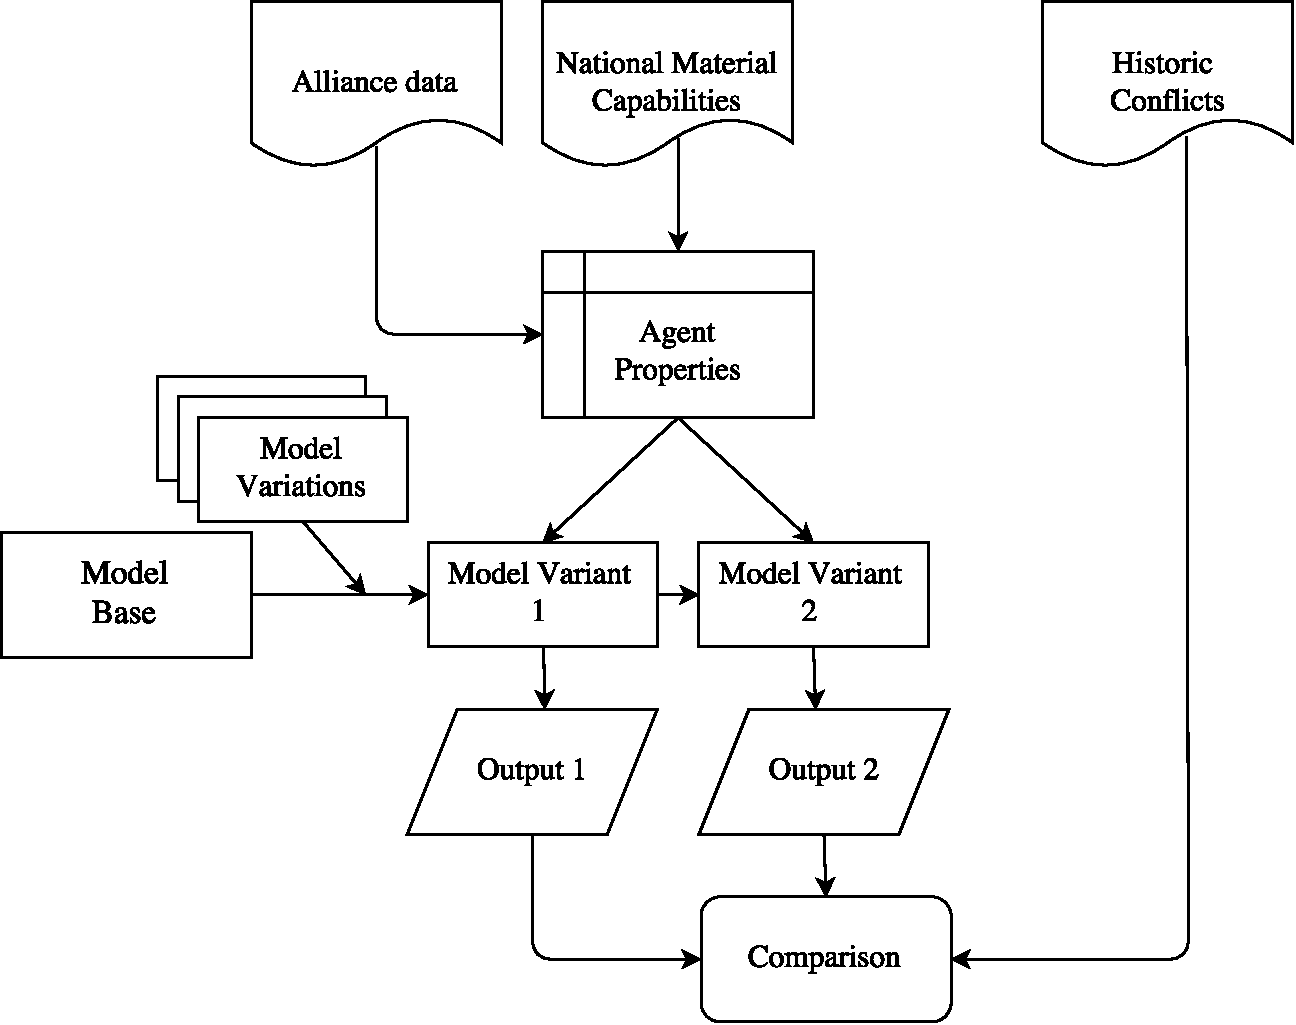
\includegraphics[width=0.75\textwidth]{figures/ModelFlowChart}
    \caption{Modeling Methodology}
    \label{fig:architecture}
    \figSpace
\end{figure}

The two models I reimplement and adapt are the International Interaction Game (IIG) \citep{bdm_1992,bennett_2000}, and the Expected Utility Model (EUM) \citep{bdm_1994,bdm_1997,bdm_2002}. Though I did not intend to focus on the works of Bruce Bueno de Mesquita in particular, these two models are among the few game-theoretic models that have been instantiated with data intended to capture real-world scenarios and have had their results compared to empirical data for those scenarios. Both are also amenable to implementation as ABMs: they consist of unitary actors, interacting with each other in discrete steps within a broader environment of other actors. Both are ultimately models of the actors' decisionmaking, and keep many other factors (such as the actors' coercive capabilities) exogenous. Yet both also make it possible to separate the actors' actions from the process by which they decide on them. This allows me to replace the original decisionmaking models with alternative ones based on different theories, repeat the same interactions, and see where the results correspond or diverge.

I implement both models using an object-oriented approach, keeping the sub-models as separate as possible. Each model has an overall World class which contains the agents, schedules their activation, and collects data on their interactions, where each World object is a particular model instantiation, used for one model run. The World class may also have inner classes for different sub-models. The agents are implemented such that they are comprised of two classes: the outer class stores the agents' public, common-knowledge properties, and sends and receives the interactions to the world and the other agents; the inner class controls the actual decisionmaking, storing internal, private properties and implementing methods for selecting among possible choices. This architecture allows for a clear separation between the interaction model and the decisionmaking model, and facilitates the substitution of different decision models between model instantiations.


For each model, I explore sub-model and decisionmaking variants anchored in different theories. As a baseline, I attempt to replicate the original models, and implement the  rational decisionmaking assumption they incorporate. I use the International Interaction Game to focus on agent decisionmaking, and implement two new agent models. One is driven by the idea that states, the agents in the model, make decisions using standard operating procedures \citep{allison_1999,levy_1986} which are updated based on simple feedback from past interactions \citep{steinbruner_1976}. The second model adds organizational memory, which the agents use to store the lessons learned from each previous interaction \citep{march_1993}; when facing a new interaction, the agents draw on the lessons of the most analogous past case \citep{khong_1992,schuman_1992}. Within the Expected Utility Model, I focus on the model's theory of coercion: embedded in the original model is an assumption that actors can use their power to directly impose their preferences on others, rather than simply inflict costs if their demands are not met. I implement and test a variant which brings the model in line with the understanding of coercion described by \citet{schelling_1966}. Other variants I implement bring the agents' risk acceptance sub-model in better line with Prospect Theory \citep{kahneman_1984,mcdermott_2001}, test the effect of the sequence of agent actions, and allow the agents to attempt to balance between potential threats.

Both the IIG and EUM have been applied to explain historic international conflicts, and in fact to see whether they could predict them from earlier data. In \citet{bdm_1992} the IIG is applied to European country dyads from the years 1816-1970, which is extended to all global dyads between 1816 and 1992 in \citet{bennett_2000}. Similarly, \citet{bdm_1998} instantiates the EUM with data on world and regional powers in 1948, and attempts to predict the course of the Cold War between the United States and Soviet Union. In both cases, the models' output is compared to data on the corresponding actors and period, with the similarity between them provided as empirical evidence that the models are effectively capturing relevant elements of the real world. Importantly, \citet{stokman_1994b} directly compare the outputs of early EUM implementation \citep{bdm_1994} with those of another model, the \citet{stokman_1994} Logrolling Model, which is instantiated with the same input data as the EUM but implements very different theoretical assumptions -- namely, that outcomes are reached via multi-issue compromises rather than coercion. I apply a similar methodology, and extend it in two ways. For each model variant, I run multiple instantiations in order to generate a distribution of outcomes which I can describe and explore. I also investigate the application of the EUM to machine-coded high-resolution political event data: to the best of my knowledge, the first such application. By comparing the output of each model to the empirical data, I can not only assess their fit individually but compare them to one another. If one model variant generates outputs which fit the empirical data better than another, this is evidence that the theories the variant implements have more explanatory and predictive power than the ones the other is based on. Similarly, if two variants have similar predictive power, it suggests that neither is necessarily more correct than the other.

Simply attempting to reproduce the results of previous models can be a valuable test, and provide a new perspective on the previous results (and indeed, in Chapter 3 I discuss the implications of failing to reproduce prior results). Additionally, this research provides several novel contributions. By anchoring agent-based models to accepted and well-studied models in international relations, I demonstrate that ABMs are not necessarily a separate and alien methodology in the discipline, but can be utilized as an extension to established research tools. In fact, as I will argue in Chapter 3, the EUM appears to be best understood as an ABM itself rather than a formal game-theoretic model. Furthermore, ABMs can implement theories of behavior which heretofore have been difficult to examine outside of resource-intensive case studies, allowing them to be tested statistically and comparatively on large-scale data.To summarize several conclusions, I find that non-rational theories have similar explanatory power to the theory of rational behavior, and that the \citet{schelling_1966}-based coercion sub-model yields better predictions in the EUM than the original version.

This research also advances the discipline of agent-based modeling itself in several ways. It demonstrates the value of designing models to be modular, in order to facilitate experiments incorporating different sub-models but controlling for other factors. It further demonstrates how such models can be anchored to real data, and how such data can be used to comparatively test the explanatory power of model variants, and the theories they operationalize. As I argue in Chapter 3, this is particularly important when models are not simply operationalizations of previous supported theories, but are themselves a new theory or hypothesis about the system being modeled. In this way, it extends \citet{epstein_2008}, utilizing ABMs for prediction not as a way of knowing the future but as a test of the underlying theory. Chapter 2 represents, to the best of my knowledge, the first application of reinforcement learning to a multi-agent model of agents dyadically playing an extensive-form game -- a narrow combination, to be sure, but one with relevance that likely goes beyond international relations. Indeed, though my substantive focus here is on international relations, the overall methodology of extending formal models into agent-based ones, implementing different sub-model variants, and testing them comparatively against empirical data, is likely applicable across other social science fields as well. This also contributes to the predictive game theory research agenda presented by \citet{fudenberg_2010}.

\section{Data Sources} \label{data-sources}

An important feature of the work in this dissertation is that it utilized historic, real-world data, both to provide the model inputs and to test the outputs. Several data sources will recur across chapters, and are thus worth examining in detail.

The majority of the datasets I use here originate from the Correlates of War (COW) project. This project is an informal collaboration of scholars who since 1963 have been facilitating the collection and dissemination of datasets useful for understanding wars and their causes \citep{cow_2016}. These datasets have become a primary tool in the quantitative study of conflicts, and of international relations more broadly. While there are several more detailed and specific datasets of interstate relationships \citep[e.g.][]{hendrix_2013,raleigh_2010}, there are no others with comparable breadth of scope. Applying the COW datasets to the computational models I present here is particularly fitting. In the first paper summarizing the project's early years, \citet{singer_1972} described the project's long-term ambitions: 
\begin{displayquote}
``[T]he natural next step would be [the conversion of analytical sub-models] to computerized, dynamic form. Then, by representing the most promising and powerful of these limited models as sub-routines of an ultimately integrated large-scale computer model, we can move to parameter estimation and sensitivity testing in a particularly effective fashion.''
\end{displayquote}

The first dataset used to derive inputs across all three chapters is the Formal Alliances dataset \citep{singer_1969,gibler_2009}. This dataset collects formal, written defense-oriented agreements between pairs of countries, including the dates that each agreement started and ended. Information on these treaties is collected from a variety of historical sources \citep{gibler_2004} and coded manually into several categories, with a spot-checking procedure used to ensure consistent coding. The most recent version of the data codes four categories of alliances, from defensive pacts requiring one party to intervene militarily if the other is attacked, to ententes which may merely pledge consultation when one party faces a crisis. 

In the models I present here, alliance data is generally not used directly -- that is, states are not necessarily assumed to come to the aid of allies they have defensive pacts with, for example. Instead, the models follow the approach introduced by \citet{bdm_1975} and treat alliances as indicators of states' unobserved interests. The more similar the sets of alliances of two states (their alliance portfolio), the closer their interests are considered to align. This similarity is estimated via Kendall's rank correlation coefficient (Kendall's tau-b) \citep{abdi_2007}.

The next dataset is the National Material Capabilities (NMC) \citep{singer_1972,singer_1988}, an estimation of states' `hard power' \citep{wilson_2008}, their military and coercive capabilities, for each year. The NMC data consists of six indicators: population size, urban population, energy consumption, iron and steel production, military expenditure, and number of military personnel. These indicators are then aggregated into a single Composite Index of National Capability (CINC) by averaging each state's share of each indicator for all states in the dataset for that year. This normalizes the data across the different units of measurement, and gives equal weighting to each indicator. It also means that CINC provides a measure of relative strength, which is only valid within a particular year. This data is collected from a variety of historic sources, as detailed in the most recent codebook \citep{grieg_2010}; when data for a particular year is unavailable, it is estimated or interpolated. The indicators are intended to estimate the CINC rather than be used on their own; as such, the data collection methodology is directed towards broad data sources which allow direct comparison between states rather than narrower, more precise specific estimates which cannot necessarily be directly aggregated or compared.

The two datasets above are used primarily as model inputs. The main dataset I will compare the model outputs to is the Militarized Interstate Disputes dataset \citep{palmer_2015}. Militarized Interstate Disputes (MIDs) are cases where one state threatens or uses military force against another\footnote{Strictly speaking, MIDs are such cases which fall short of war; however, the MID dataset itself includes wars as well.}. The dataset is human-coded from media and historic sources, and records the states involved in each dispute, noting which are the initiators. For each case, the dataset includes several variables coding the intensity of the conflict on each side, in particular the highest category of hostility reached by each side -- from threat of force through declaration of war. I use this dataset as the ground truth for empirical crises and conflicts, and will measure the various models' power to predict them.

Additionally, in Chapter 3 I experiment with using more detailed event data, consisting of machine-coded media records of individual actions taken by governments and other politically-relevant actors. Each event consists of a source, a target, an action, a timestamp (generally a day) and possibly a location: more colloquially, who did what to whom, when, and where. An important advantage of event data is that it captures the micro-level dynamics of conflicts, as well as the normal patterns of activity when conflicts are not occurring. There are several different event data sets available, including the Global Data on Event, Location and Tone (GDELT) \citep{leetaru_2013} and the Phoenix data system \citep{schrodt_2014}, both of which update on a daily basis; and the Integrated Crisis Early Warning System (ICEWS) \citep{boschee_2015} dataset, a US government-funded system which updates daily but is only made available to the public on a year's delay. Among the datasets with global, daily coverage, Phoenix remains relatively untested, and ICEWS has been assessed as more reliable than GDELT \citep{ward_2013}. For this reason, I choose to utilize ICEWS in order to explore whether Expected Utility Model variants can predict the volume of conflict events between different international actors. 

\section{Organization of the Dissertation}

The body of this dissertation is in the following three chapters. Chapter 2 is intended to stand on its own; Chapters 3 and 4 and more closely related, with Chapter 4 utilizing the Expected Utility Model variants described in more detail in Chapter 3, and serving to provide additional validation.

In Chapter 2, I focus on modeling the decisionmaking of states in bilateral crises, using the International Interaction Game. I restate the model as described in \citet{bdm_1992} and \citet{bennett_2000}, and describe how I reimplement it as an agent-based model. Using this implementation, I introduce a notional model I will use to test the agent decision sub-models, using simplified agent properties and payoff calculations and a reduced game tree. Two new decisionmaking models are presented, which can be applied to these games: one is a pure reinforcement learning model, meant to capture a stylized version of states' learning and application of standard operating procedures which guide their decisionmaking in crises; the other adds a case-based reasoning component to the reinforcement learning model, representing how decisionmakers utilize lessons learned from previous similar interactions when facing new crises. Agents are endowed with both decisionmaking models, first in the notional simplified model and then in the IIG using data on historic dyads and disputes. I compare the outcomes of the games utilizing those two decisionmaking models to the rational equilibria, and measure the degree to which the agents collectively learn to reach equilibria outcomes. Finally, the IIG model results are compared to the historic observed event associated with each interaction, and estimate whether these models provide a better explanation of them than the equilibria.

In Chapter 3 I describe the Expected Utility Model, and my implementation of it as an ABM. I focus on identifying the sub-models the EUM is composed of, at both the level of agent decisionmaking (where agents choose what actions to take towards one another), and at the level of the model `world' (how the agents' actions are sequenced, and how conflicts are resolved). The chapter describes the assumptions embedded in these sub-models, many of which are not explicitly articulated in the original descriptions of the models, and builds on those by proposing and implementing alternatives. I generate notional instantiations in order to conduct a sensitivity analysis and quantify the uncertainty captured by the original model, which has not previously been well-studied. Finally, six model variants are instantiated, each comprised of a different combination of sub-model variants, with input data drawn from the Correlates of War datasets for key world powers in 2004; each model variant is run multiple times, in order to test whether the conflicts generated by the models are useful predictors for ICEWS conflict events for the years 2005-06 following the input data. This allows for a comparison off the predictive power of the various model variants, which in turn provides evidence for which ones are the best models of the actual underlying dynamics between the real actors.

Chapter 4 extends the analysis of the EUM as a tool for modeling international relations by attempting to replicate, and expanding on, the model's previous application to simulate the course of the Cold War \citep{bdm_1998}. The original paper proposes that, contra \citet{gaddis_1992}, the end of the Cold War did not violate established theories of international relations, but can be understood as emerging from them -- and that a model, such as the EUM, can capture the complex interactions which lead to its emergence. The procedures described in the original paper is repeated in order to generate model input data from the Correlates of War datasets and to compare the new results to the originals. I then run two variants of the EUM: my reimplementation of the model described in \citet{bdm_2002}, and the model variant identified as having the most predictive power in the ICEWS analysis in Chapter 3. Multiple instantiations of each are run, using both the original and updated inputs, and collect the conflicts generated by each run. Following the methodology in \citet{bdm_1998}, I examine the resulting distribution of outcomes, and sample agent position traces which lead to each, comparing them to historic intuition about the dynamics of the Cold War. Additionally, I test whether the the conflicts generated by each model are a useful predictor of the number of MIDs recorded for each dyad. Finally, I analyze the distances between agents at the end of each model run, and test whether they are useful predictors of the alliance network observed in 1998, corresponding to the model's end-point.

Finally, Chapter 5 concludes the dissertation. I summarize the results of the previous chapters, and discuss their broader implications. With these findings in hand, I can more concretely describe how this work forwards the broader comparative analysis and agent-based modeling research areas, and propose  extensions and experiments which can further build on the work presented here.

\chapter[Learning and War]{Learning and War: Applying Learning Models to the International Interaction Game}

\section{Background}\label{background}

An important topic in the study of international relations is how the actors in the international system (primarily countries) make decisions when interacting with one another. One common view, most often associated with the Realist schools of thought \citep{sep_2013} is that states\footnote{I will use states and countries interchangeably to refer to sovereign, territorial political entities.} are rational: they act in a way that attempts to maximize their utility, often defined as security from the threat of attack by other states \citep{keohane_1986}. Many critiques of Realist theories, particularly from the Liberal perspective \citep[e.g.][]{keohane_1987}, focus on disputing the constraints and goals faced by states and on whether states are even the correct actors to concentrate on, but not that the relevant actors themselves are rational. Nevertheless, there has also been substantial scholarship arguing against the idea of states as rational, goal-directed actors, focusing both on the differing objectives and relationships of the internal actors involved in the decisionmaking process \citep{singer_1961,wendt_1987,allison_1999}, and on the psychological biases of the individuals who are, ultimately, the ones making the decisions \citep{north_1967,jervis_1976,khong_1992,kaufmann_1994}.

Crises, and the precipes of conflict between countries, are particularly important phenomena. The decision to threaten or use force is one of the most consequential external decisions a state may make, and the substantial costs and consequences of wars at the national and human levels make them compellingly important to study, explain, and possibly even predict or avert. In ``The Essence of Decision,'' \citet{allison_1999} closely examined one particularly important example: the 1962 Cuban Missile Crisis, in which the world's two superpowers, the United States and the Soviet Union, faced a series of decisions to initiate or escalate a military confrontation with one another that had a real possibility of leading to a nuclear exchange. The book reviews three models of state decisionmaking: rational choice, where the decisionmakers attempt to evaluate various possible courses of action and choose those which have the highest expected utility, while taking the adversary's responses into account; organizational behavior, wherein the states' decisions are driven by standing institutional procedures; and governmental politics, in which decisions are driven by competition between internal factions and actors with different interests and degrees of influence. The book demonstrates that all three models can provide convincing explanations of the behavior of the United States and Soviet Union over the course of the crisis, and in particular that the latter two models can explain actions that do not make sense as strategic, security-maximizing decisions. Similarly, \citet{kaufmann_1994} conducted a detailed case study of another international crisis, the 1905-06 Moroccan Crisis (wherein Germany attempted to undermine French influence in Morocco and brought Europe to the brink of war), and used archival sources to argue that the key German decisionmakers updated their views and positions during the crisis in response to events and new information in a way that is inconsistent with pure rationality, but consistent with the psychological biases expected to affect them.
% WGK: Consider breaking up EoD models into bullet points or something?

Both of these examples demonstrate the power of comparative analysis of different decisionmaking models, and especially the application of multiple models to the same case. However, both share a reliance on qualitative analysis of detailed primary sources detailing not only the ultimate behavior of the state-level actors but the internal deliberations of their decisionmaking individuals and organizations. This makes it difficult to test these models across different cases, or to use them to make broad hypotheses as to the conditions under which we can expect conflicts or predict how they will be resolved. In this, they are nearly the complete opposite of game theory, perhaps the other methodological pole in the study of international relations. 

Game theory is the mathematical study of models of interactions (games) between multiple actors (players), where the payoff each player receives depends on the combination of their own actions and those of the other players. Game theory generally takes utility-maximizing rationality as axiomatic; this allows games to be analyzed in order to identify and characterize their equilibrium -- the outcome of a game when all players are perfectly rational, know that the other players are perfectly rational as well, and figure out the best possible course of action given that the other players are doing the same thing. Recently, however, behavioral game theory \citep{camerer_2003} has sought to use experiments and psychological insights to study how humans actually approach such games, and how their behavior differs from theoretical, rational expectations.

%Much of modern game theory was developed in order to study international conflict \citep{gates_1997}.  Game theory takes utility-maximizing rationality as axiomatic, and much of the work of game theory involves studying games (formal models of interaction) in order to identify and characterize their equilibrium -- the outcome of a game when all players are perfectly rational, know that the other players are perfectly rational as well, and figure out the best possible course of action given that the other players are doing the same thing. Game-theoretic models tend to be highly abstract, and may provide useful analogies and theory-generating insights rather than specific explanations or predictions applicable to a particular case \citep{snidal_1985}.

% RAX: Slightly awkward introduction to game theory -- rewrite to explicitly emphasize game theory as the font of rational modeling; maybe note behavioral game theory?
% RAX: Cite Gintis on game theory as a general social science?

Game-theoretic models tend to be highly abstract, and may provide useful analogies and theory-generating insights rather than specific explanations or predictions applicable to a particular case \citep{snidal_1985}. An important exception is included in ``War and Reason'' by \citet{bdm_1992}, which presents the International Interaction Game: a game-theoretic, extensive-form model of inter-state crises. The game consists of two agents sequentially choosing whether to escalate confrontation or attempt to deescalate, with outcomes ranging from the maintenance of the status quo (when neither actor escalates at all) to war (when both actors escalate as far as possible). While much of the book is devoted to conventional formal analysis of the model and its equilibria under different parameters, the authors also test the theory empirically. They propose a methodology to estimate the game's payoffs for any given pair of states, using data on the states' alliances to measure the conflict stakes,  and states' material capabilities to measure the strength each side and its allies can bring to bear. Using this methodology with historic data from the Correlates of War project, they estimate the game payoffs for 707 historic European dyads (pairs of countries in a particular year) from the 1816-1970 time period. They find the equilibrium outcome for each, and show that these outcomes are useful predictors of the corresponding event observed between those countries for that year. \citet{bennett_2000b} developed a software tool expanding the estimation to all historic dyads across the entire international system between 1816 and 1992, largely confirming that the estimated equilibria can be used to predict the observed event for the corresponding dyad -- though the strongest predictions required controlling for distance, great power status, and other relevant factors.

Agent-based models have seen relatively limited use in the study of international relations, and have generally been applied similarly to game-theoretic models. Many \citep[e.g.][]{cederman_1997,axelrod_1997,min_2002} involve simulations of notional, simplified international systems, with agents acting in accordance with some particular theories. These models provide stylized insights into what patterns emerge (or do not) from these theories, but are not meant to directly describe specific real-world countries or conflicts. One important example is the \citet{axelrod_1980} Prisoners' Dilemma Tournament, which explicitly sought to compare the performance of different behavior rules playing an iterated game. While this research utilized a simple theoretical model, it was done with an eye towards the study of, among other issues, international conflict and cooperation. Similarly, though less robustly, \citet{cederman_1997} involves competition between agents with two sets of behavioral rules, those content with the status quo and those seeking to expand at the expense of their neighbors. These experiments demonstrate a powerful feature of agent-based models, which has heretofore been underutilized in political models: the ability to have agents using different behavior models interact and compete with one another within a common context.

While it is not presented as such, the \citet{bdm_1992} empirical application of the International Interaction Game bears some similarity to an ABM. Indeed, the empirical application of the model is only feasible computationally. It consists of distinct, unitary actors with well-specified decision rules, carrying out discrete interactions with one another. These interactions, in turn, generate a series of cooperative and conflictual behaviors, which can be compared to empirical data. Nevertheless, as previously implemented by \citet{bdm_1992} and \citet{bennett_2000,bennett_2000b}, the agents (such as they are) only feature a single decisionmaking model, rationally playing the equilibrium moves. The way I will extend the International Interaction Game (IIG) should now be clear: I propose to reimplement the model explicitly as an agent-based model, and to do so in a way that allows me to endow agents with  different decisionmaking models and rules, drawn from different theories of state behavior. Utilizing the IIG game tree and payoff estimates keeps the model anchored to a well studied, empirically validated foundation. I then use this framework to simulate the same set of interactions using different decisionmaking models, obtaining sets of outcomes for each variant. These outcomes can be compared to one another to see where and how they differ, and to empirical data, to see which provides the best fit.

% RAX: Cite Green & Shapiro (green_1994, pathologies... rat. choice) here?

In this framework, formal rationality will be the initial decisionmaking model I will implement. As discussed above, this is the default model of decisionmaking used in game-theoretic models. It serves as an operationalization of the qualitative rational choice model as described by \citet{allison_1999} and many others. The analysis in \citet{bennett_2000} compares the explanatory power of the overall IIG to dyad-level variables (e.g. geographic distance, government types) but not to other models of decisionmaking. Here, in contrast, using rationality as a baseline will allow us to directly test whether the additional decisionmaking models provide stronger explanatory power than the rational decisionmaking model itself. Furthermore, reimplementing the rational choice model will serve as a form of verification, ensuring that my model framework is producing the same results as the \citet{bennett_2000,bennett_2000b} implementation.

I implement two alternative models of decisionmaking within this framework. The first variant is a stylized representation of the organizational procedure model described by \citet{allison_1999} and \citet{levy_1986}: agents develop standard operating procedures, which they apply regardless of the specifics of each interaction they find themselves in. These procedures are updated based on the outcome of the new interaction, such that successful courses of action will be more likely to be executed in the future, and unsuccessful ones less likely.

The second variant implements a stylized version of the theory described by \citet{march_1993} and \citet{khong_1992} by which organizations, and states in particular, make decisions by comparing their present circumstances to previous similar cases they encountered. In this variant, the agents maintain a library of past interactions, which they draw on to make decisions about each new interaction. If a course of action was successful in a similar previous interaction, the agent will be more likely to use it again; otherwise, they will be more likely to attempt an alternative.

These decisionmaking models are both implemented using reinforcement learning. This methodology has several advantages: it originates from psychology, but has had success as a machine learning technique \citep{sutton_1998}. Reinforcement learning agents have been shown to be capable of learning to play extensive-form games \citep{laslier_2005,akramizadeh_2009}, as well as to learn to cooperate and compete in multi-agent environments \citep{littman_1994,claus_1998}. They have been used to model the learning of individuals and groups of decisionmakers \citep{kocher_2005}; however, they are not always successful at learning to play the equilibrium of abstract, normal-form games, and in fact can yield unexpected and even chaotic behavior \citep{galla_2013}. Furthermore, \citet{khong_1992}, \citet{allison_1999}, and \citet{cederman_2001} have observed that states as a whole (rather than just individual decisionmakers) exhibit a degree of learning from past experiences. In short, reinforcement learning provides a plausible, general model of decisionmaking which is not procedurally rational \citep{simon_1976}, but introduces minimal additional assumptions as to the form the behavior takes. Additionally, reinforcement learning makes minimal assumptions as to the structure of the game the agents are playing, meaning that a single behavior model may be implemented once and used to drive agents across different games and other interaction models. %% Add citation for temporality in IR?

The question I set out to explore here is whether reinforcement learning agents interacting with one another over a series of simulated international crises can converge to behavior resembling the equilibria for those interactions. If this is the case, it will suggest a degree of convergence between the rational choice, psychological, and organizational models of decisionmaking. If it is not, however, it will diverge, generating different results which may then be tested against empirical data. In the course of addressing these questions, I will also lay out a more general architecture and methodology for extending game-theoretic models of international crises into agent-based models, which can be used to implement and test additional models of decisionmaking. As \citet{allison_1999} write, ``because  simplifications are necessary, competing simplifications are essential.'' In this chapter, I will present a methodology for extending the competing simplifications from the realm of case studies to computational modeling.

This chapter is organized as follows. In Section \ref{description}, I present the general architecture for an agent-based model of dyadic, extensive-form interactions with variable agent decisionmaking. I describe two simulated worlds: a simplified, notional international system (Section \ref{small_crisis}), and a more complicated data-grounded historic simulation based on \citet{bdm_1992} and \citet{bennett_2000} (Section \ref{sec:iig_description}). I then present several behavior variants, grounding them both in political and multi-agent theory (Section \ref{decisionmaking_models}). In Section \ref{small_crisis_results}, I apply these behavior variants to the notional model and verify their behavior, and then apply them to the full historic data in Section \ref{iig_results}. I compare their behavior to the purely rational decisionmaking, and to the observed historic outcomes of each simulated interaction.

\section{Model Description} \label{description}

The overall model I present here consists of three sub-models intended to capture distinct levels of phenomena: the `World' consisting of a set of agents with certain properties, which may be fixed or change over time; the Interaction sub-model, consisting of an extensive-form game tree for pairs of agents to play against each other; and the Agents themselves. The Agent class, in turn, is composed of two parent classes: the World Agent, which defines the properties and methods specific to the World, and a Decisionmaking Model, which the agents utilize to play the extensive-form game at each interaction. All these sub-models are implemented initially as abstract classes, which include the methods common across all model variants; these abstract classes are then sub-classed and implemented for each model variant. Figure \ref{fig:model_architecture} shows a UML class diagram tying together these different classes.

\begin{figure}[h!]
    \centering
	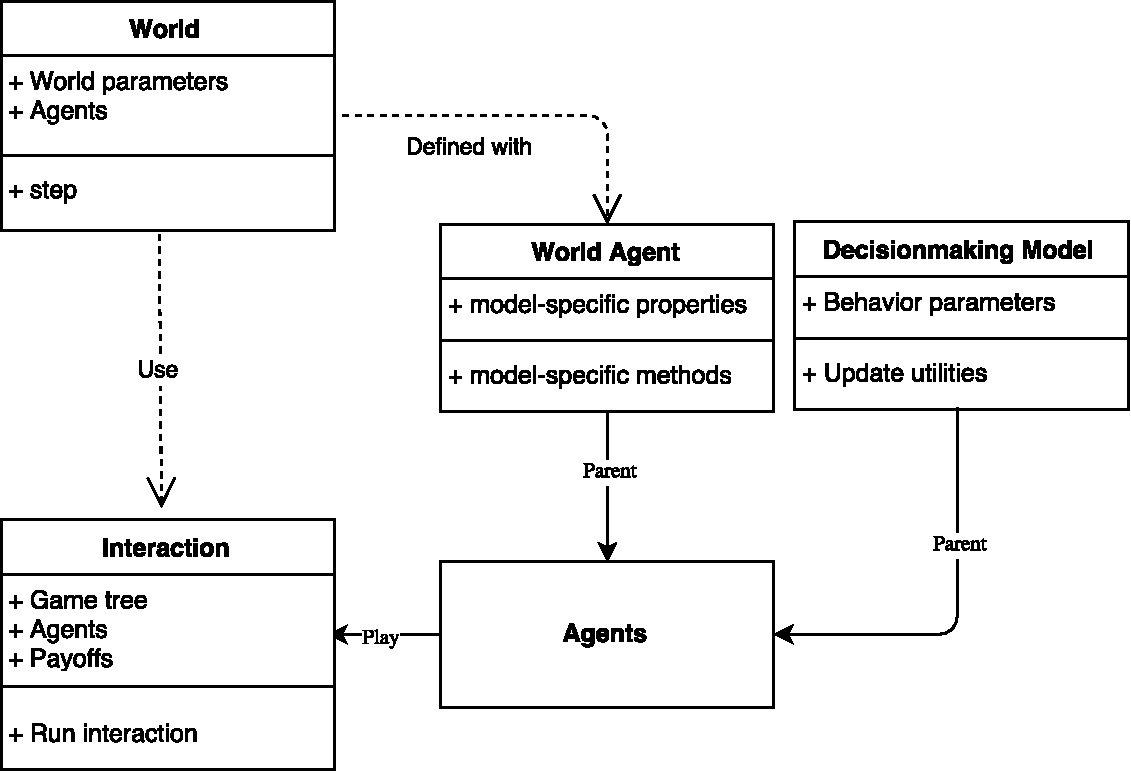
\includegraphics[width=0.75\textwidth]{WarReason/Figures/ModelArchitecture}
    \caption{Model Architecture}
    \label{fig:model_architecture}
    \figSpace
\end{figure}

\subsection{World Sub-Model}

The World sub-model acts as the overall controller for the entire model. It stores and manages the agents who will interact with each other over the course of each instantiation, generating a particular notional history. A World is instantiated with a set of agents, as well as a subclass of the generic Interaction sub-model class, described below. The World implementation can also accept additional data used to generate agents, schedule their interactions, and store and export the outcomes of those interactions.

The World's key method is the `step', which advances the model by one simulated year, chosen since that is the level at which the IIG data is available. Each year consists of some set of interactions, depending on the model variant. For example, these may be some number of random pairings of agents, all possible agent dyads, or pairings based on crises occurring in the given year as recorded in the input data. The agents do not directly choose with whom or when to interact; the interaction scheduling is exogenous to the agents themselves. Since the player order matters in extensive-form games, the interaction dyads are directed -- that is, an interaction between A and B is not the same as one between B and A.

Finally, the World also collects and stores data on each agent, and on the result of each interaction -- that is, which terminal node the interaction ended up on, as explained below. A World implementation may also perform some evaluation on this interaction outcome. In particular, the World sub-models I develop compare the outcome of each interaction to that interaction's equilibrium outcome.

\subsection{Interaction Sub-Model}

This is the core of the overall model: a single interaction between agents playing through a standard, two-player, extensive-form game \citep{shoham_2009}. An interaction model is implemented with a game tree, and methods for computing the payoff to each agent at each terminal node. The game tree here is assumed to be a direct, acyclic graph with perfect information (that is, there are no information sets of more than one node, and agents know exactly the node where the game is currently). The player agents take turns in fixed order, and there are also no moves by nature.

Each agent has a step method, which takes the interaction state as an input and emits a move. The sub-model makes sure that the move is valid for the current node, and advances the game's current node to the appropriate result of the given move. If this is a terminal node, the interaction is over, and payoffs are distributed to all the agents. Otherwise, the next player agent is called.

I use two game trees here, which are shown in Figures \ref{fig:small_crisis_tree} and \ref{fig:iig_tree}. The simpler one is drawn from \citet{signorino_1999}, and will be used for the notional model; the more complicated one is from \citet{bdm_1992} and will be applied to the historic data. The utility calculations associated with both will be provided in more detail in the appropriate sections below.

\subsection{Agent Sub-Model}

Finally, there are the agents themselves. Each agent is meant to represent one actor in the international system, as they interact with one another as described above. Each agent class has two parent classes, as shown in Figure \ref{fig:model_architecture}: one is the World Agent, for the particular model variant which provides its properties; the second is the Decisionmaking Model, which contains the methods and properties the agent uses to make decisions at each step of the game. All agents in a given World must have the same World Agent parent, which is compatible with the Interaction sub-class. However, different agents within a world may have different decisionmaking parents.

In general, the agent properties deriving from the model variant parent class are used to compute the utilities the agent expects from each terminal node in the game tree. The decisionmaking parent, in turn, provides the `step' method, with which the agent chooses its next move through the game tree during an interaction. This structure allows decisionmaking rules to be modeled once, verified, and applied across different specific interaction and world models with minimal additional development. 

\section{Model Variants}

I present two model variants below. Each one consists of an implementation of the three sub-models described above: a World, Interaction model, and agent properties. The first variant, the Small Crisis Game, is a simple notional model used for testing the agent behaviors under controlled conditions. The second, the International Interaction Game, is a full model of the international system extending \citet{bdm_1992} and \citet{bennett_2000b}, at a level of one agent per state, attempting to capture historic interaction dyads.

\subsection{Small Crisis Game} \label{small_crisis}

This model variant is a purposeful simplification: in the number of agents, their properties, and the game tree of their interactions. It is adapted from \citet{signorino_1999}, which in turn adapts the game tree shown in Figure \ref{fig:small_crisis_tree} from the game trees in \citet{bdm_1992}, as well as \citet{kim_1995} and \citet{fearon_1995}. At every node of this game tree, agents (Players 1 and 2, or P1 and P2) may escalate the conflict (fight, $F$) or refrain from escalating (not fight, $!F$). If neither agent chooses to escalate, the result is the Status Quo; if one agent escalates, the other agent faces a choice between not escalating and yielding to the escalator's demand (Capitulating), or fighting, leading to War. These outcomes are the tree's terminal nodes.

The payoffs associated with these terminal nodes are dependent on agent properties. Each agent $i$ in this model is defined by its Assets ($a_i$), indicating what they have that other agents might want (whether territory, material, or more abstract positions or concessions); their Capability ($c_i$), indicating the strength they have to coerce other agents and defend themselves from coercion by others; and a Bloc ($b_i$), where two agents are geopolitically aligned (and have more incentive to cooperate) if their Bloc properties match. These properties are used to compute the utilities associated with each terminal node, as shown in Table \ref{table:smallcrisis_utils}. These utilities are also adapted from \citet{signorino_1999}: when agents capitulate, they yield the assets being contested, with the other agent gaining them. If the agents enter into conflict, they will win with probability based on the ratio of their capability to the other agent's; if they win, they secure the other agent's assets -- and if they lose, they lose not only the value of their own assets, but of their expended capability as well. The Status Quo leads to no change in utility if the agents belong to different blocs; however, if the agents belong to the same bloc, cooperation (i.e. not entering into conflict) has a positive payoff\footnote{In \cite{signorino_1999}, there is a Democracy property instead of a Bloc property, with only dyads of democracies receiving the cooperation payoff; the form I present here is more general, and does not introduce the assumption of democratic peace. However, initial experiments using the original specifications produced substantively similar results to the ones I present here.}.

\begin{figure}[h!]
    \centering
	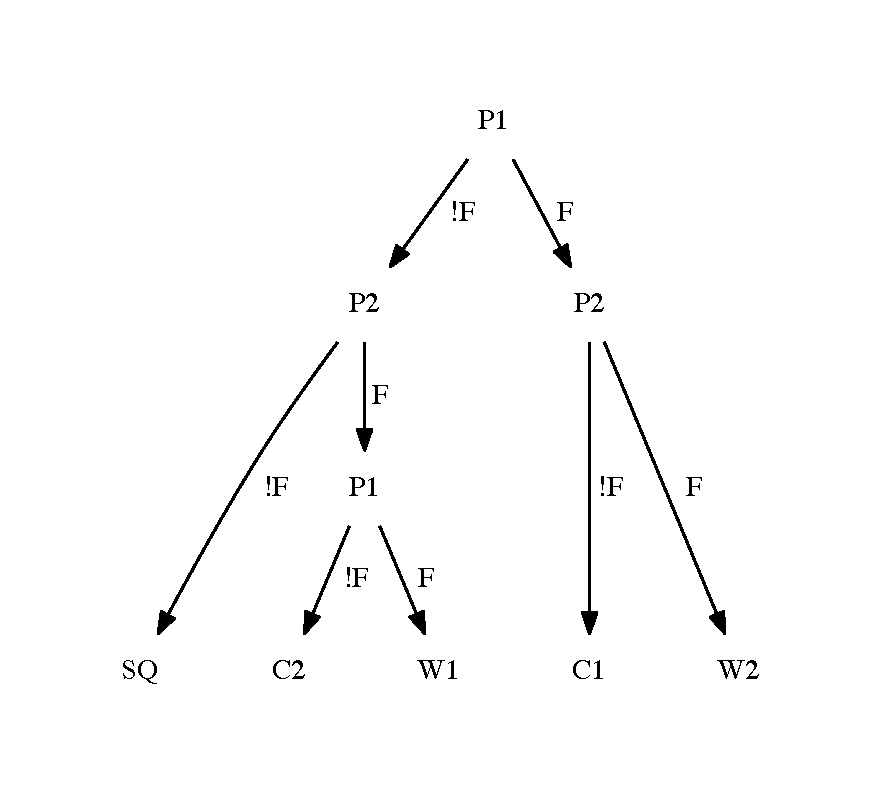
\includegraphics[scale=0.75]{WarReason/Figures/SmallCrisisTree}

    \caption[Small Crisis Game Tree]{Small Crisis Game Tree \citep[adapted from][]{signorino_1999}}
    \label{fig:small_crisis_tree}
    \figSpace
\end{figure}


\begin{table}[h!]
\centering
  \caption{Small Crisis Model Utilities}
  \label{table:smallcrisis_utils}
\begin{tabular}{lll}
	\hline
	Node 			& $U_1$ 		& $U_2$ \\
	\hline
	Status Quo (SQ)  	& $20\delta(b_1,b_2)$			&	$20\delta(b_1,b_2)$			\\
	Capitulate 1 (C1)	& $-a_1$						& $a_1$							\\
	Capitulate 2 (C2) 	& $a_2$							& $-a_2$						\\
	War 		 (W1, W2)	& $p_1a_2 + (1-p_1)(-a_1-m_1)$  & $p_2a_1 + (1-p_2)(-a_2-m_2)$	\\
	\hline
	$p=$Prob(win)	& $\frac{c_1}{c_1+c_2}$ 	   	& $\frac{c_2}{c_1+c_2}$			\\
	\hline
\end{tabular}
\tableSpace
\end{table}

For every instantiation of the CrisisWorld, $N$ agents are generated at random, with random properties drawn uniformly as shown in Table \ref{table:agent_properties}. These agents will persist across the entire run; that is, agents are not added to or removed from the model instance. In each instantiation, all agents will share the same decisionmaking model, as specified below.

Each year of the model (that is, a step of the world), all the agents will be paired up, in random order. Since the number of agents being simulated is substantially smaller than the total number of agents in the international system, this can be thought of as representing a particular region (analogous to the focus on European dyads in \citet{bdm_1992}), or a subset of politically-relevant actors within a larger system.

\begin{table}[]
\centering
	\caption{Small Crisis Agent Properties}
  	\label{table:agent_properties}
\begin{tabular}{lll}
	\hline
	Property & Distribution 	 & Change  	 \\
	\hline
	$a_i$	 &	$Unif\{1, 100\}$ & $\mathcal{N}(0, 5)$   \\
	$c_i$	 &	$Unif\{1, 100\}$ & $\mathcal{N}(0, 5)$	 \\
	$b_i$	 &	$Bernoulli(0.5)$ & $1 - Bernoulli(0.05)$ \\
	\hline
\end{tabular}
\tableSpace
\end{table}

I create two variants of the Small Crisis model. In the first, the Static variant, the agent properties are fixed across each run. In the second, the Dynamic variant, the properties of each agent change stochastically at the beginning of every simulated year, with the changes distributed as shown in Table \ref{table:agent_properties}. This means that under the first variant, the utilities (and hence the equilibrium) of an interaction between each dyad of agents are constant, whereas in the second variant they may drift from step to step.

Note that the agent attribute values do not change due to the results of their interactions. While this is a simplifying assumption, it also corresponds to the dynamics observed in the National Material Capabilities dataset \citep{singer_1988,grieg_2010}, wherein the majority of conflicts do not substantially impact states' estimated material capabilities or alliance relationships -- which are used in the empirical International Interaction Game to operationalize the capabilities of states and the stakes of conflict, respectively, as described below.

\subsection{International Interaction Game} \label{sec:iig_description}

The International Interaction Game, as described in \citet{bdm_1992} is as follows. It involves two actors, one who initiates the interaction and one who responds. The game proceeds following a tree, as shown in Figure \ref{fig:iig_tree}. As in the simplified model, at each node the actors (Players 1 and 2, P1 and P2) have a choice between two moves: escalating the confrontation (fight, $F$) or not escalating ($!F$). There are more nodes in this tree, leading to a wider range of outcomes. If neither actor escalates, the result is still the Status Quo, while if both consistently escalate the result is War. If one agent yields to the other's escalation early on, the outcome is Acquiescence, while if they yield after a greater degree of escalation, the outcome is Capitulation, with some additional cost incurred. If both actors initially escalate and then deescalate, the result is a negotiated compromise. 

\begin{figure}[h!]
    \centering
	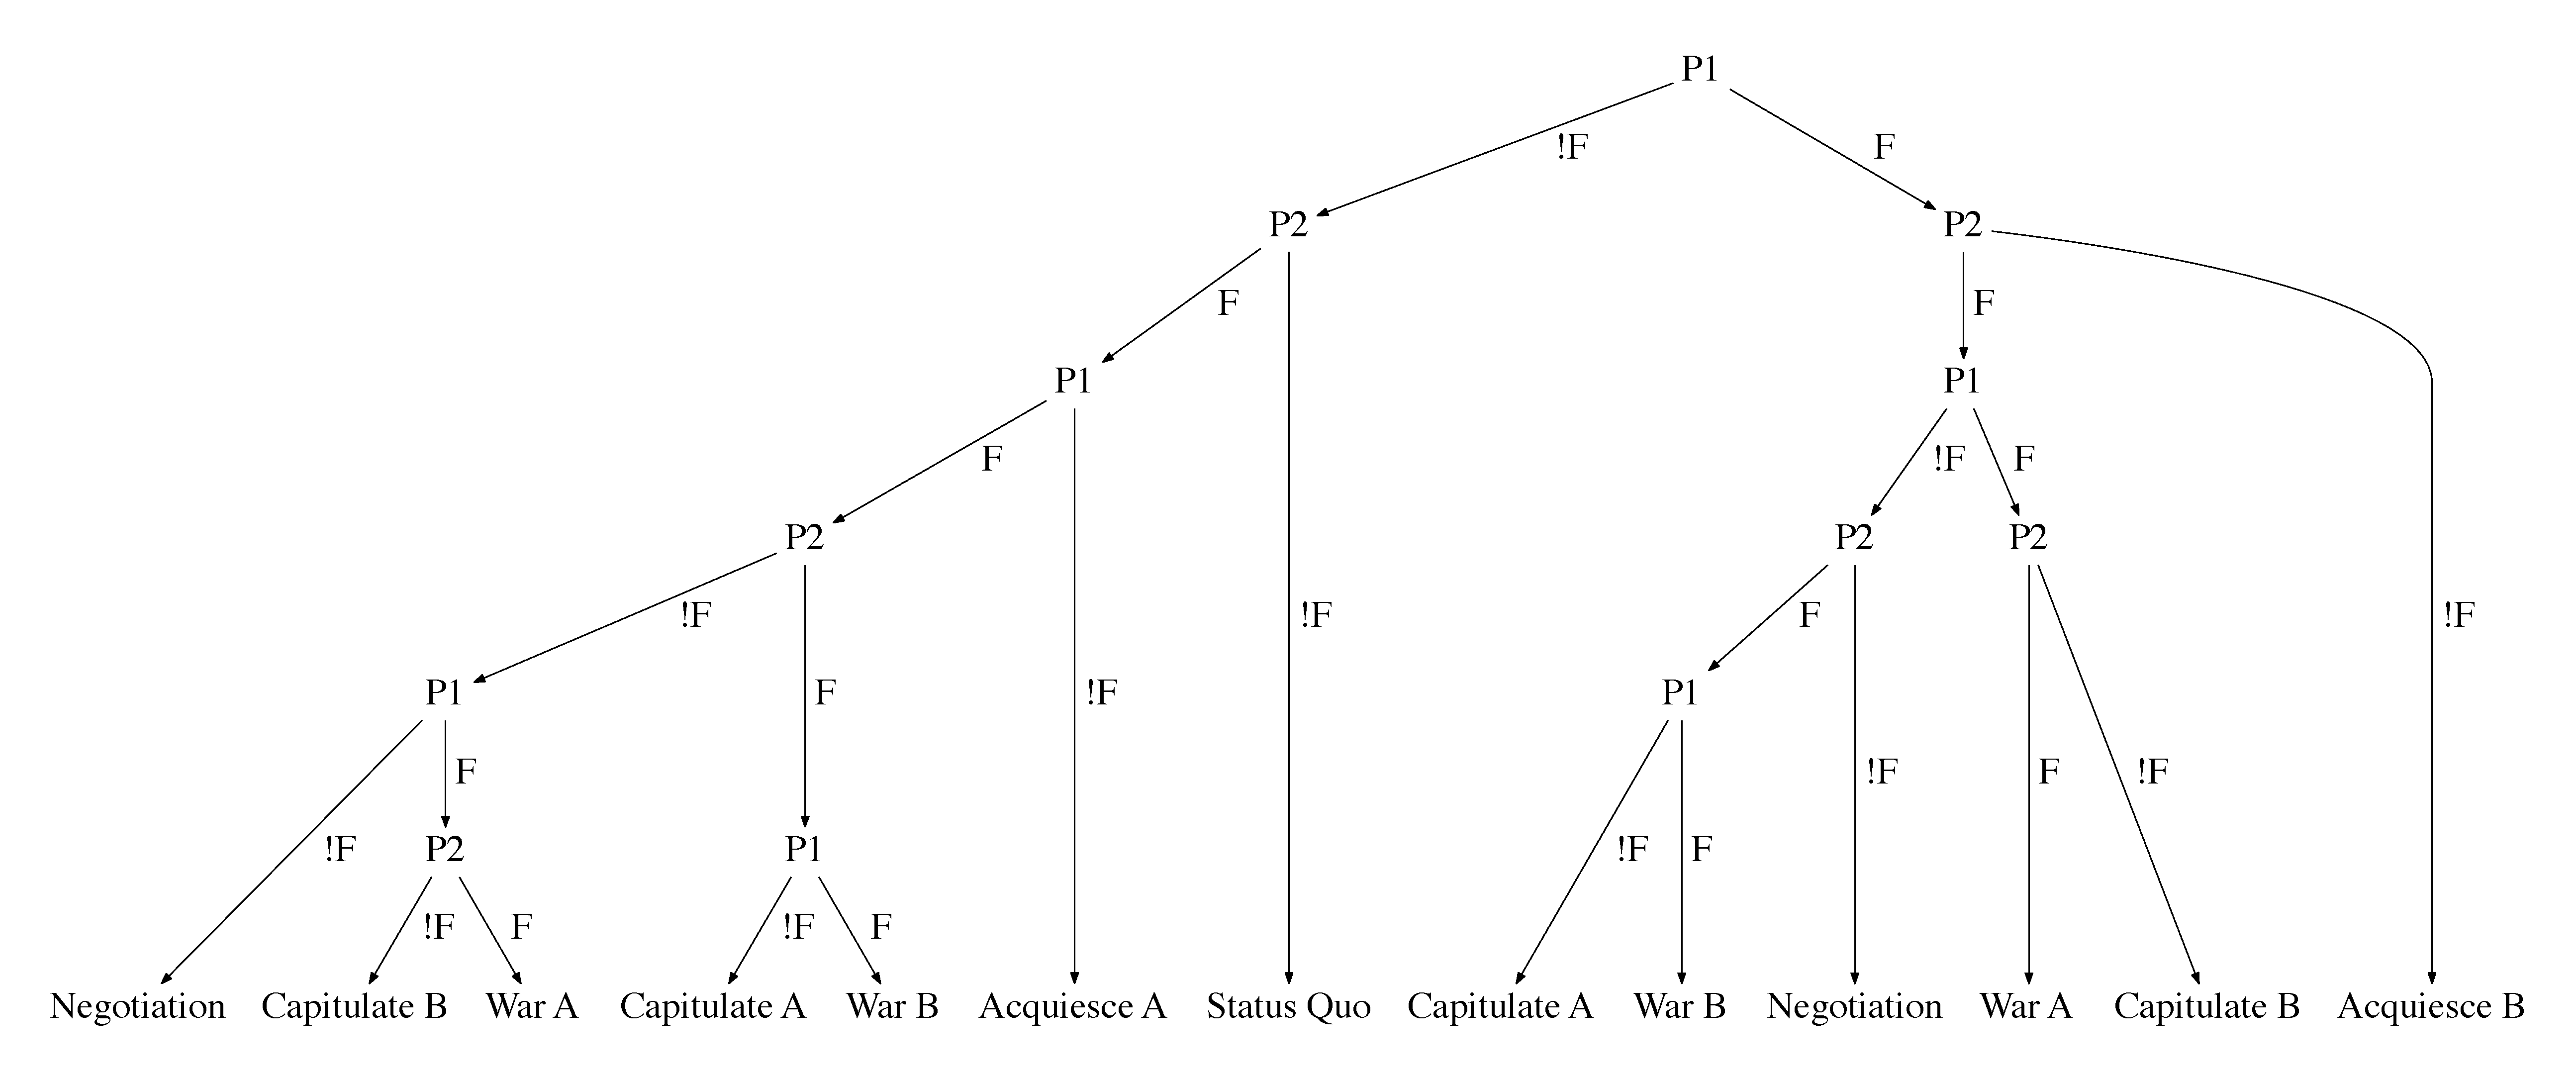
\includegraphics[width=\textwidth]{WarReason/Figures/IIGTree}

    \caption[International Interaction Game Tree]{International Interaction Game Tree \citep[from][]{bdm_1992}}
    \label{fig:iig_tree}
    \figSpace
\end{figure}

While each interaction is dyadic, the utilities of each outcome for both actors are determined by the overall international system the interaction occurs within, and specifically the network of alliances. Alliances are used as a proxy for states' interests. The COW alliance data \citep{singer_1969} records the type of each formal alliance each state has with any other state in a given year; this is that state's alliance portfolio. As \citet{bdm_1975} argues, two states with similar interests can be expected to have similar alliance portfolios -- that is, many of the same types of alliances with the same other states. \citet{bdm_1992} uses a standard statistical similarity measure known as Kendall's tau-b to compute this similarity, though \citet{signorino_1999b} argues that this measure is inadequate, and proposes an alternative. To maintain consistency with \citet{bdm_1992} and \citet{bennett_2000}, I will use Kendall's tau-b, denoted below as $K_{i,j}$ -- the similarity between actors $i$ and $j$'s alliance portfolios. However, other similarity measures, such as those proposed by \citet{signorino_1999b} may be substituted as well.

The estimated similarity between the two states is used to determine the two base utility rates for the corresponding actors, under the assumption that the more dissimilar two states' interests are, the more each has to gain or lose from a conflict. $U^A(\Delta_A)$ is Actor $A$'s utility if its own objective is achieved, and $U^A(\Delta_B)$ is its utility if the other actor $B$ achieves its objective instead.

\begin{align} 	
	U^A(\Delta_A) = 2 - 4 \left(\frac{2-(1-K_{B,A})}{4}\right)^{r_A} \label{eq:u_a1}\\ 
	U^A(\Delta_B) = 2 - 4 \left(\frac{2-(K_{B,A}-1)}{4}\right)^{r_A} \label{eq:u_a2}
\end{align}

Where $r_A$ represents each actor's risk tolerance, also estimated from the alliance network as described in \citet{bdm_1985} and \citet{bennett_2000b}\footnote{\label{fn:eugene_risk}Risk tolerance is computed by comparing an agent's total probability of victory in all possible conflicts (as detailed below in Equation \ref{eq:prob_win}) to the maximum and minimum possible total victory probabilities, across all possible alliance portfolios. This is by far the most computationally intensive step; the \citet{bennett_2000b} EUGene software, which implements the IIG, uses pre-computed results from a single six-month optimization done using genetic algorithms. This methodology is also almost certainly yielding an inaccurate estimate. Recent work such as \citet{maoz_2010} and \citet{cranmer_2012b} shows that alliances are best understood as mutually dependent network edges, meaning that they ought not be permuted independently as was done here. A better methodology would estimate risk tolerance from structurally plausible networks only, which would likely have the added advantage of greatly reducing the search space. However, a full implementation of this methodology is outside the scope of this dissertation, and must be left for future work. Additional future work along the same lines may also conduct a sensitivity analysis on risk tolerance in order to estimate the degree to which different values lead to substantively different equilibria or behavior.}.

If the two actors have identical alliance portfolios, and hence approximately identical interests, they will both be indifferent as to who will `win' a confrontation -- meaning that a confrontation will certainly not occur.

In addition to these utilities, the international alliance network determines each actor's probability of prevailing in negotiations or war, based on the support they can muster from the rest of the actors in the system. Specifically, it determines their \emph{perception} of their probability of prevailing. For each actor in the international system, the model computes their own interest in the bilateral conflict under consideration, based on the similarity of that actor's alliance portfolio to the two parties to the conflict. They then allocate some of their resources, estimated by the COW National Material Capabilities index \citep{nmc_2010} to one side or the other. Agent A's estimate of Agent C's preference for A over B is:

\begin{align} 	
	Pref_A^C(A,B)=\frac{K_{C,A}-K_{C,B}}{2}\exp(R_A(K_{C,A}-K_{C,B})) \label{eq:pref_c}
\end{align}

($R_A$ is a rescaling of $r_A$). 

Then, each actor in the conflict has a probability of prevailing equal to its share of the total resources allocated. Agent's A's perception of its probability of prevailing against Agent B is:

\begin{align} 
	P^A=\frac{\sum_{c\in\Psi}\Lambda^c Pref^A_c(A,B) }{\sum\Lambda^c Pref^A_c(A,B)} \label{eq:prob_win}
\end{align} 

Where $\Lambda^c$ is c's capabilities (operationalized as NMC) for every actor $C$, and $\Psi$ is the subset of actors who prefer $A$ to $B$ (that is, $Pref_A^c(A,B)>0$). Note that this formulation is similar to the model of bilateral conflicts found in the multilateral expected utility model \citep{bdm_1997,bdm_2002,scholz_2011} described in further detail in the following chapter.

Note the $R^A$ term in Equation \ref{eq:pref_c}  -- this is the risk tolerance factor of one of the actors in the conflict, not the third-party actor who may be contributing resources. This is implicit mirror-imaging, a perception documented intelligence in both the cognitive \citep{meltzoff_2003} and political senses \citep{heuer_2001}  where the actor assumes that everyone shares its own attitudes, in this case towards risk. What Equation \ref{eq:prob_win} is capturing, then, is not an objective probability of victory in a possible conflict, but each actor's own perception of this probability. Thus, the utilities appearing below are agent A's expected utilities from each outcome.

Using these probabilities, we can finally write the utilities for all the outcomes of the IIG, which are:

%\begin{flalign} 
\begin{align} 
	U^A(StatusQuo) &= 2-4(\frac{2}{4})^{r^A} \\ 	
	U^A(Acqiesce_B) &= U^A(\Delta_A) \\ 
	U^A(Acqiesce_A) &= U^A(\Delta_B) \\ 
	U^A(Negotiate) &= P^AU^A(\Delta_A) + (1-P^A)U^A(\Delta_B) \\ 
	U^A(Capitulate_B) &= U^A(\Delta_A)-P^A \\
	U^A(Capitulate_A) &= U^A(\Delta_B)-(1-P^A) \\
	U^A(War) &= P^A(U^A(\Delta_A) - P^A - (1-P^A)) + (1-P^A)(U^A(\Delta_B - P^A - (1-P^A)) 
%\end{flalign}
\end{align}

%\begin{equation}
%\begin{split}
%	U^A(War) &= P^A(U^A(\Delta_A) - P^A - \\
%	 (1-P^A)) + (1-P^A)(U^A(\Delta_B - P^A - (1-P^A)) 
%	\end{split}
%%U^A(War) = P^A(U^A(\Delta_A) - P^A - (1-P^A)) + (1-P^A)(U^A(\Delta_B - P^A - (1-P^A)) 
%\end{equation}

Using the methodology described above, \citet{bdm_1992} test the IIG model by computing the utilities and finding the equilibria for 700 dyads between European countries. \citet{bennett_2000} extended this analysis by developing the EUGene (Expected Utility Generation) software tool\footnote{Code and binaries available at \url{http://www.eugenesoftware.org/}}, which is capable of computing utilities for all possible dyads in the international system based on the then-current versions of the Correlates of War datasets \citep{sarkees_2000,jones_1996}. EUGene also modifies the form of the probability of victory in Equation \ref{eq:prob_win} to account for states' declining ability to project force over greater distances. Finally, as mentioned in Footnote \ref{fn:eugene_risk}, EUGene includes pre-computed risk tolerances, which are prohibitively expensive computationally to reestimate\footnote{The task of estimating a single actor's risk tolerance for a single year requires finding the best and worst alliance portfolios it may hold; this is conceptually very similar to the optimization performed in fitting exponential random graph models, which has been shown to be \#P-hard \citep{bannister_2014}. This optimization must then be performed for each actor in each year, for a total of approximately 15,000 times.}.

While the Correlates of War project has since updated its datasets from the ones used by \citet{bennett_2000b}, yielding slight changes particularly in the alliance networks used to estimate utilities and risk coefficients, I continue to use the EUGene output for this analysis. This serves two purposes: it allows me to directly compare my results to previous ones relying on the same data; and it allows me to concentrate on the comparative behavioral modeling as opposed to the utility calculations. However, future work utilizing the methodology described here for more accurate historic comparison and forecasting should probably recompute the utilities from more recent and complete data.

The EUGene software generates a dataset of 1,610,478 rows, with each row a country dyad by year. I filter out those rows for which, for various reasons, the EUGene model could not compute utilities for those pairings, leaving 1,027,692 rows. Each row of the dataset represents two actors playing the international interaction game at a particular point in time, with particular interests and in a particular context. Each row records the conflict event, if any, that occurred between the two actors in that year; the event categories correspond to the terminal nodes in the IIG tree (see Figure \ref{fig:iig_tree}) and are categories based on the level of military force each actor used against the other, as detailed in \citet{bennett_2000b}. Since the levels of force are sequential, each one corresponds approximately to an escalation move in the IIG. This assumes that each directed dyad of states will have at most one crisis per year. In the majority of cases, neither side will have used any military force against the other, corresponding to a Status Quo outcome.

The World sub-model creates one agent for each unique state which appears in the dataset, as identified by the country code variable. These agents persist across the entire model instantiation. This is a simplifying assumption, which assumes continuity for countries which may have experienced radically different governments over their lifetimes; however, it is in line with the approach of \citet{bdm_1992} and \citet{bennett_2000}, and indeed of the COW data itself which does not distinguish between different regimes presiding over the same state.

In agent-based modeling terms, we can use this dataset as the agent scheduler, iteratively advancing through the table and running the Interaction sub-model for the dyad of agents in each row. By default, the data is sorted by year, and then first and second agent country codes. While the year ordering is obviously temporal, the code ordering is not. Since the decisionmaking models presented here are path-dependent (agents learn from the outcome of one interaction, influencing their decisions in the next interaction) it is important to reduce the effect of potential artifacts of particular interaction sequences. In order to do so, the rows of the data table are shuffled within each year for each instantiation. The model then loops over the shuffled rows. For each row, it retrieves the agents specified in that row, and has them play the IIG, with the payoffs on the terminal nodes specified in the row. Note that this implicitly introduces the assumption of one interaction (or potential conflict) per directed dyad per year; however, again, this assumption is in line with the approach taken by \citet{bennett_2000}, and indeed with the way the COW data itself is organized \citep{palmer_2015}. Finally, and most problematically, since states' attributes are taken directly from the data, this methodology assumes that the particular outcome of each interaction does not directly change them. For example, if an interaction results in a War outcome when in reality the states remained at Status Quo for that dyad-year, the war will not change the agents' capabilities or alliances. This is a simplifying assumption, to be sure, but allows us to focus on modeling the decisionmaking itself, rather than developing and incorporating additional models of the material and multilateral consequences of wars.
% RAX: Is this similar to microsim 'alignment'? 
%A: Alignment seems to be more about modifying output to align closer to data, which we don't do here.

Figure \ref{fig:data_by_year} shows the number of new states present in the dataset each year, and the number of interactions between them. Since the number of potential interactions goes as the square of the number of states, it is not surprising that the number of interactions per year increase substantially in the latter part of the dataset. Model results below will be reported by annual averages for ease of historic intuition and to account for in-year shuffling; but it is important to keep in mind that later years will include more interactions than earlier years.

\begin{figure}[h!]
    \centering
	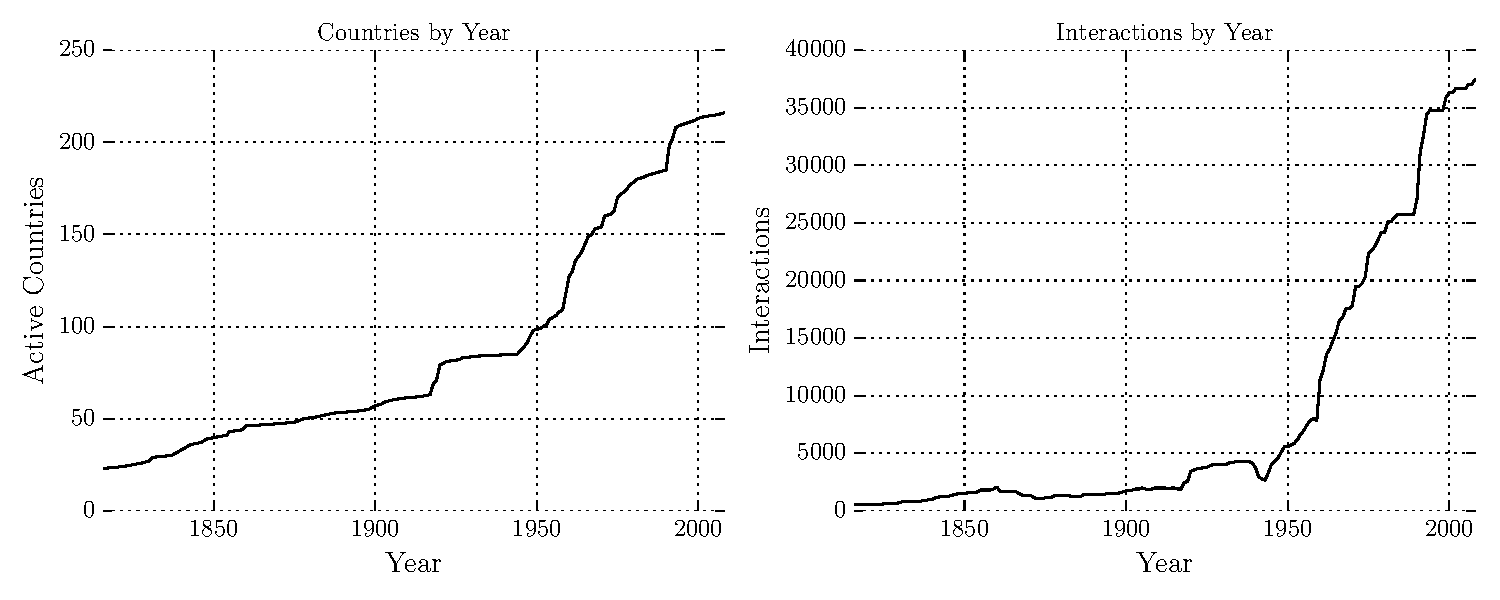
\includegraphics[width=\textwidth]{WarReason/Figures/DataByYear}
    \caption{EUGene Data by Year}
    \label{fig:data_by_year}
    \figSpace
\end{figure}


This methodology allows us to run an agent-based model against historic data. Each agent interaction within each model instantiation corresponding to a particular observed or potential interaction, and the outcome of the model interaction can be compared to the event observed for that interaction. Importantly, as agents only are influenced by their previous interactions, each model outcome is an out-of-sample prediction.

\section{Decisionmaking Models} \label{decisionmaking_models}

Agents in the two models described above have different properties and interact with each other via different games. Over the course of the interactions themselves, however, the agents face the same structure of an extensive-form game, where they must choose one of several moves at each node, with a final payoff depending on the moves both they and their counterpart have made. In most applications of game theory, this model is implicitly perfect rationality; in practice, the equilibrium is found not by agents but by the external modeler (with the so-called gods'-eye view of the situation). The architecture of the agent-based framework I have developed and described here requires an agent-level implementation of any decision rule, including rationality. Any such implementation operationalizes a theory or set of theories of actor decisionmaking.

The framework I describe here makes a few high-level assumptions as to the agent decisionmaking models. The agents have access to the current node of the game, and know all the possible actions they may take at that node. The rational agents described below have access to the full game tree, including the various node payoffs. I also assume that all interactions within a given model implementation share the same game tree structure. Finally, agents do not have direct access to the decisionmaking model of the other agent.

In this section, I describe the three decisionmaking models I implement. The first is classic rationality with perfect information, which serves as a baseline. The second and third are simple reinforcement learning, and a case-based reasoning extension; both use an experience-weighted attraction implementation so that the actual decisions are stochastic, and vary based on how the attraction weights associated with each move are chosen and updated. In the Reinforcement Learning (RL) decision model, the agents maintain a single set of attraction weights, which they use for all interactions. In the Case-Based Learning (CB) decision model, agents maintain a library of weights learned from past cases, and for each interaction select the weights associated with the most similar past case.

In the next section (Section \ref{experiments-and-results}) I apply these decision models to the Small Crisis Model and International Interaction Game, described above. My initial hypotheses are that, as suggested by previous work on reinforcement learning \citep[e.g.][]{laslier_2005,akramizadeh_2009,galla_2013}, both the RL and CB models will converge to producing outcomes equal to the rational model's (the equilibrium outcomes) more often than we would expect purely at random; I also expect the CB model to outperform the RL model and result in more common equilibrium outcomes, since it adds a degree of coarse-grained strategic reasoning, with agents adjusting their behavior based on their counterpart in each interaction -- implicitly anticipating that agent's own decisions.

\subsection{Rational Model}\label{original-spe-model}

Before implementing additional model variants, I start by reproducing the original rational decisionmaking model. Rational agents have full access to the game tree, and both agents' utilities at each terminal node. They identify the subgame-perfect equilibrium by backwards induction \citep{russell_2009}, finding the correct moves for both players to make at each node and propagating the corresponding utilities up the tree. This leads to a best-response move at all nodes of the tree, not just those that are on the main equilibrium line; thus, even when playing against an opponent who is not playing the equilibrium moves, this agent will be able to choose the game-theoretic best response. In the remainder of this chapter, the equilibrium of an interaction is defined as the result of the interaction when played between two such rational agents.

\subsection{Weighted-Attraction Agents}\label{weighted-attraction-agents}

The game-theoretic model of rationality described above is not time dependent: the particular history of the agent does not matter; the agents, already perfectly rational, do not learn. Furthermore, the agents' decisions are wholly deterministic. Finally, the agents have full awareness of where they are in the game tree, and are capable of planning ahead to the end of the tree, see the plan through, and costlessly replan if the other agent deviates from their expectations.

The two decisionmaking models that follow all begin from different assumptions. In describing the organizational model of decisionmaking, \citet{allison_1999} note that, contrary to the rational model's assumption of perfect lookahead, ``[o]rganizations exhibit great reluctance to base actions on estimates of an uncertain future,'' and instead prefer to utilize existing procedures. As \citet{levy_1986} describes, military organizations in particular tend to prepare plans and procedures which may be inflexibly put into practice in crisis situations. Organizations in general, as \citet{lundberg_1995} reviews, tend to learn in the form of adopting new routines based on past experiences. Finally, \citet{march_1993} note that organizations do not necessarily seek the optimal course of action, and often satisfice -- find a course of action which meets some threshold of acceptability. I distill these characteristics into the following assumptions:

\begin{itemize}
 	\item The agents play the game myopically, choosing each move without explicit look-ahead in the game tree.
 	 \item The agents' choice of move at each node is based on their past experience.
 	 \item At the end of each interaction, the agents only have knowledge of the actual outcome, and cannot directly compare it to the `road not taken.' 
 \end{itemize}

These assumptions are implemented via experience-weighted attraction (EWA), a particular form of reinforcement learning \citep{sutton_1998,galla_2013}. At each node of the game tree, agents associate a certain weight with each potential action they can take. They choose among the actions stochastically, in proportion to the weight they place on each. If the weights are equal, all actions may be chosen with equal probability; if one action has overwhelmingly more weight than the others, it will be chosen with probability approaching 1. These weights are learned based on the agent's past experiences, and in particular the utilities they gained at the end of previous interactions. The specific ways the weights are learned are explained in the subsections below. 

This model form is taken proximately from \citet{galla_2013}, who in turn adopt it from several other sources \citep{camerer_2002,kocher_2005,ho_2007}. Most importantly for our purposes, the experimental results reported by \citet{kocher_2005} indicate that EWA is an effective model for strategic learning not just by individuals but by groups tasked with making a decision jointly.

Formally, the model is as follows. Within a particular interaction, an agent $i$ has an attraction function $ Q_i : s_{x,k} \mapsto w$ which maps from $s_{x,k}$, a move available at node $x$, to a numeric weight $w$. In practice, this is implemented as an associative array, with node-move tuples as keys and weights as values. At node $x$, the agent chooses move $s_{x,k}$ with probability:

\begin{equation}
    P_i(s_{x,k}) = \frac{exp(\beta Q_i(s_{x,k}))}{\sum_{s_{x,m}}exp(\beta Q_i({s_{x,m}}))}
\end{equation}

Where $\beta$ is a fixed parameter which further weights the choice weights. When $\beta=0$, all moves are equally likely regardless of weight. The larger $\beta$ is, the more likely a move with a smaller weight advantage is to be chosen. In general, I set $\beta=1$ for all agents; however, as this is an agent-level parameter, there is nothing preventing agents from having heterogeneous $\beta$ values.

In Python-style pseudocode, the agent class's EWA method is implemented as follows:

\begin{singlespace}
\begin{lstlisting}[language=python,caption={Experience-Weighted Attraction},label={code:ewa}]
def step(model):
    current_state = model.current_node
    choices = {}
    for move in model.tree[current_state].children:
        choices[move] = self.Q[key]
    choice = self.weighted_choice(choices, self.beta)
    self.past_moves.append((current_state, choice))
    return choice
\end{lstlisting}
\end{singlespace}

This decision framework can be thought of in several ways. It can simply represent the relevant decisionmakers' view of the relative merit of each possible course of action \citep{kocher_2005}. It can also represent the relative influence or credibility of different factions or sub-actors advocating for different courses of action, or standing procedures developed by the relevant organizations, such as reserve call-ups or troop movements \citep{levy_1986}. How to interpret it will rest partially on the particular learning rule, which will determine how the weights are learned and updated between interactions. The two learning rules I use are described next.

\subsection{Pure Reinforcement Learning}\label{pure-reinforcement-learning}

This model variant is the closest to traditional EWA, as described in \citet{galla_2013} and elsewhere. Under this decisionmaking model, agents choose actions based on their total past experiences, without taking into account any of the properties of the specific agent they are interacting with, or the broader environment. At the end of every interaction, agents update their attraction to each move they made based on the payoff they received. Moves which led to higher utilities will be more likely to be played again, while ones that led to lower utilities (and in particular, to negative utilities) will be less likely to be played again.

In terms of crisis behavior, this variant can be thought of as a stylized version of the organizational procedure model described by \citet{allison_1999}. The agents are developing `standard operating procedures' they will follow without evaluating their appropriateness for the particular crisis they are facing at the moment. When the crisis is resolved, they will update their procedures based on the crisis's outcomes. To be sure, this is an exaggerated view of the organization procedure model, as nobody claims that states act solely on the basis of preset, inflexible procedures. Yet if so, it may also be no more exaggerated than the game-theoretic operationalization of the rational choice model.

Formally, each agent has a single experience table $Q_i$, encoding the utility it has gained from making decisions at each node in the past. This experience table drives the decisionmaking at each node of the game tree, until the interaction ends. At that point, the table is updated at the end of the interaction with the corresponding utility.

At the end of an interaction, let the set of moves agent $i$ has decided to play be $S_i = \{ s_{x_0,k}... s_{x_l,k} \}$ for each node in the game tree. Let $\Pi _i$ be the payoff associated with the terminal node reached by $S_i$ and $S_j$. The updating rule is then:

\begin{equation}
    Q^{t+1}_i(s_{x,k} \in S_i) = \alpha \Pi _i +  (1-\alpha) Q^{t}_i(s_{x,k}) 
\end{equation}

Parameter $\alpha$ is the learning rate, where $\alpha \in {[0, 1]}$. When $\alpha=1$, the agent has effectively no memory, and associates a move only with its most recent payoff. Conversely, if $\alpha=0$ the agent never updates its attraction weights. In practice, obviously, this value will be somewhere in between these extremes. The $\alpha$ value is set by the modeler; I will explore its effects in Section \ref{small_crisis_results}.

This model differs from some other, similar models, in that it attempts to capture realistic learning from experience rather than serve as an optimization algorithm. Thus, it does not incorporate fictitious play \citep{shoham_2003}, and agents have no ability to access other potential payoffs from decisions not taken. Importantly, due to this, the weights on moves not taken do not update, meaning that entire branches of the game tree may be unaffected by a particular interaction where play does not pass through that branch. Similarly, the weight on any move not taken is not updated; thus, whether a particular update will substantially change the probability of a move being chosen in the future depends not just on the move's own updated weight, but the weight present on the moves not chosen.

In Python-style pseudocode, the agent's experience update method is provided below. Note that this uses the \emph{past\_moves} list updated in Code Block \ref{code:ewa}.

\begin{singlespace}
\begin{lstlisting}[language=python,caption={Reinforcement Learning},label={code:rl_update}]
def add_utility(utility):
    for move in self.past_moves:
        self.Q[move] *= (1 - self.learning_rate)
        self.Q[move] += self.learning_rate * utility
\end{lstlisting}
\end{singlespace}

\subsection{Case-Based Learner}\label{case-based-learner}

In the previous model variant, agents' past experiences were undifferentiated: the agents maintain and update a single experience table across all their interactions. This means that in a new interaction, the agent will utilize the same decision weights whether facing, for example, a strong ally or a weak rival. However, individuals and organizations are capable of maintaining and recalling and utilizing discrete memories of specific circumstances they have previously encountered. \citet{gilboa_1995} argue that case-based reasoning provides a cognitively plausible model of how individuals reason under uncertainty; similarly, \citet{march_1993} describe one of the modes of organizational decisionmaking as choosing actions based on recognizing a given situation's similarity to previously-encountered ones stored in organizational or individual memory, and retrieving rules associated with those situations. In the context of international crises and conflicts, the relevant situations are most often prior crises and conflicts. Historic analogies help shape decisionmakers' view of the stakes of a crisis, as well as the probabilities and risks associated with various courses of action \citep{khong_1992}. These analogies influence the public debate surrounding potential conflicts \citep{schuman_1992,noon_2004,schuman_2006}, as well as the strategies and tactics which may be brought to bear (e.g. \citealt{nagl_2002} and too many military `Lessons Learned' to cite). Furthermore, lessons learned from some conflicts may also lead to the reevaluation of previous conflicts (e.g. \citealt{hagerman_1992} or \citealt{forster_2002}, among many examples), sometimes exaggerated to lead to thought experiments such as a reevaluation of the American Revolutionary War in light of the lessons of the United States's Iraq and Afghanistan wars \citep{exum_2008}.

In order to model such reasoning by historic analogy, I extend the reinforcement learning model into a case-based decisionmaking model \citep{ram_1997,mantaras_2001,jiang_2009}. Instead of each agent having a single experience table, they now possess a library of such tables representing previous interactions (the cases), indexed by key salient features of each case. At the beginning of each interaction, the agents query their case library for the experience table associated with the most similar case, and use it to drive their decisionmaking for this interaction -- in other words, when facing a new case, agents approach it based on the lessons learned from the most similar previous case they have faced. At the end of the interaction, this previous table is updated, and a copy of the updated table is added to the case library, indexed at the coordinates of the current case. Thus, the lessons learned from the current case are propagated back to the previous case as well. The more frequently a case is the most-similar one, the more information (encoded as move weights) the agent has about it. This captures the fact that actors' understanding of the past is not static, and is updated based on their further experiences. While the agents in this model variant are still not `strategic' in the game-theoretic sense, they are retrieving different past experiences based on the properties (and hence, expected behavior) of the agent with whom they are currently interacting.

More formally this decisionmaking model is as follows. Let $c_i(j)$ encode a tuple of coordinates describing agent $i$'s interaction with agent $j$. Each agent $i$ has a case library of coordinates and associated attraction functions $C_i = \{(c_{i,0}, Q_{i,0}), (c_{i,1}, Q_{i,1})... \}$. When presented with a new case $c_{new}$, the agent chooses $c_* = argmin_{c \in C_i} dist(c_{new}, c)$ and the corresponding $Q_*$. $Q_*$ becomes the active attraction function for the given interaction, as described above. 

At the end of the interaction, $Q^{t+1}_*$ is updated as described above. The overall case library is then updated such that $c_* \mapsto Q^{t+1}_*$ and $c_{new} \mapsto Q^{t+1}_*$.

This decision model is implemented as follows. At the beginning of each interaction, the agent selects the active case, and corresponding experience table:

\begin{singlespace}
\begin{lstlisting}[language=python,caption={Case-Based Learning -- Set Case},label={code:cb_setccase}]
def set_new_case(coords):
    self.current_coords = coords
    self.current_case = self._get_nearest_neighbor(coords)
    self.Q = self.case_library[self.current_case]
\end{lstlisting}
\end{singlespace}

At the end of the interaction, the case library is then updated as follows:

\begin{singlespace}
\begin{lstlisting}[language=python,caption={Case-Based Learning -- Update Weights},label={code:cb_update}]
def add_utility(utility):
    for move in self.past_moves:
        self.Q[move] *= (1 - self.learning_rate)
        self.Q[move] += self.learning_rate * utility
    self.past_moves = []
    new_Q = self.Q.copy()
    self.case_library[self.current_coords] = new_Q
\end{lstlisting}
\end{singlespace}

The coordinates used for the cases are as follows:

\begin{description}
	\item[Small Crisis Model:] \begin{equation}
	c_i(j) \equiv (\Delta m, \Delta a, 100\delta(b_i,b_j))
	\end{equation}
	where $\Delta m = m_i - m_j$ and likewise for $\Delta a$, and $\delta(b_i,b_j)=1$ if $b_i=b_j$, and $0$ otherwise.
	\item[International Interaction Game:]\begin{equation}
	c_i(j) \equiv (Stakes_i, Stakes_j, P^i)
	\end{equation}
	Where $Stakes_i$ is defined in \citet{bdm_1992} as $U^i(\Delta_i) - U^i(\Delta_j)$ (see Equations \ref{eq:u_a1} and \ref{eq:u_a2}), and $P^i$ is defined in Equation \ref{eq:prob_win}.
\end{description}

\section{Experiments and Results}\label{experiments-and-results}

We now have all the necessary components in hand: two models of agent interaction, and two new models of agent decisionmaking in addition to the baseline rational model. Now we can combine them and observe the results. I first test the Reinforcement Learning (RL) and Case-Based (CB) agent decisionmaking models with the Small Crisis Model and compare their performance to one another and to the game-theoretic equilibrium. I next apply the RL and CB models to the full International Interaction Game and the EUGene data, analyze the models' behavior against both the equilibrium outcomes and the observed events, and test the model outputs' power as predictive variables. 

\subsection{Small Crisis Model} \label{small_crisis_results}
 
Before we apply the decisionmaking models to historic data, it is worthwhile to test them in a simpler, notional environment. This allowed me to test and verify the decisionmaking models themselves; as the decision trees are relatively small, and the payoff calculations straightforward, it allowed me to manually verify that the decisionmaking code matched the model descriptions, and was behaving as expected. Furthermore, this model provides a baseline against which to judge the decisionmaking models' performance. If agents in the notional system, when using decision models other than game-theoretic rationality, behave very differently from the equilibrium expectation, this leads us to hypothesize that a similar divergence should exist in reality. If, however, the agents' behavior converges to something similar to the equilibrium, it would make the real-world decision models harder to distinguish, but potentially provide support for the use of the equilibrium model -- as an approximation of state behavior rather than a direct description of it.

I carry out the experiments as follows. I instantiate Small Crisis models of 10 agents, as described in Section \ref{small_crisis}: first using the Static variants, then Dynamic one. For both model variants, I vary the learning rate $\alpha$ from 0.1 to 1, in increments of 0.1. At each parameter value, I generate 100 model instantiations. Each instantiation is done using a fixed random seed, and generates two model runs: one with agents utilizing the Reinforcement Learning (RL) decisionmaking model, and one with the Case-Based Learning (CB) decisionmaking model. Using the same random seed ensures that the random elements are fixed between the model runs -- in particular, that the agent properties are the same\footnote{In some cases, individual interactions between agents result in different-length paths through the game tree, which will lead to a divergence in the sequence of random numbers.}. The models are instantiated with agents with the same properties; these agents will interact in the same order; even the random numbers drawn when agents choose between moves will be the same. 

For each model run, I record the outcome of each interaction, as well as the equilibrium outcome for that interaction. In particular, I focus on the fraction of interactions within every simulated year where the interaction outcome matches the equilibrium outcome. I also define run quality as the mean of those fractions over the latter 50 steps of each run; this allows for a burn-in period as the agents gain initial information, discarding the early interactions where the agents' moves are approximately random. This metric allows for comparison between the behavior of the learning models and the rational model, and specifically measures the correspondence between them.

I begin with several hypotheses: first, as mentioned in Section \ref{decisionmaking_models}, that across both the Static and Dynamic variants, both the RL and CB agents will converge to near-equilibrium behavior -- that is, they will learn to play similarly to agents utilizing the purely rational decisionmaking model. I further expect that the CB agents will exhibit higher run quality (as defined above), since it allows agents to incorporate additional information and learn different weights -- that is, different likely moves -- for different interactions, implicitly incorporating a greater degree of strategic anticipation of the other agent's moves. Finally, in the Static variant, the mix of equilibria for each agent, and the equilibrium of each agent dyad, are fixed for the duration of each run, giving the agents more time to converge on the corresponding moves; in contrast, in the Dynamic variant these equilibria may change, meaning that the move weights learned from prior interactions may no longer be as likely to reach each interaction's equilibrium. Thus, I expect both the CB and RL decisionmaking models to perform worse in the Dynamic variant than in the Static one.
%% NOTE: Following paragraphs are discussing Static World Ex3, and Dynamic World Ex5.

\subsubsection{Static Variant}

\begin{figure}[h!]
	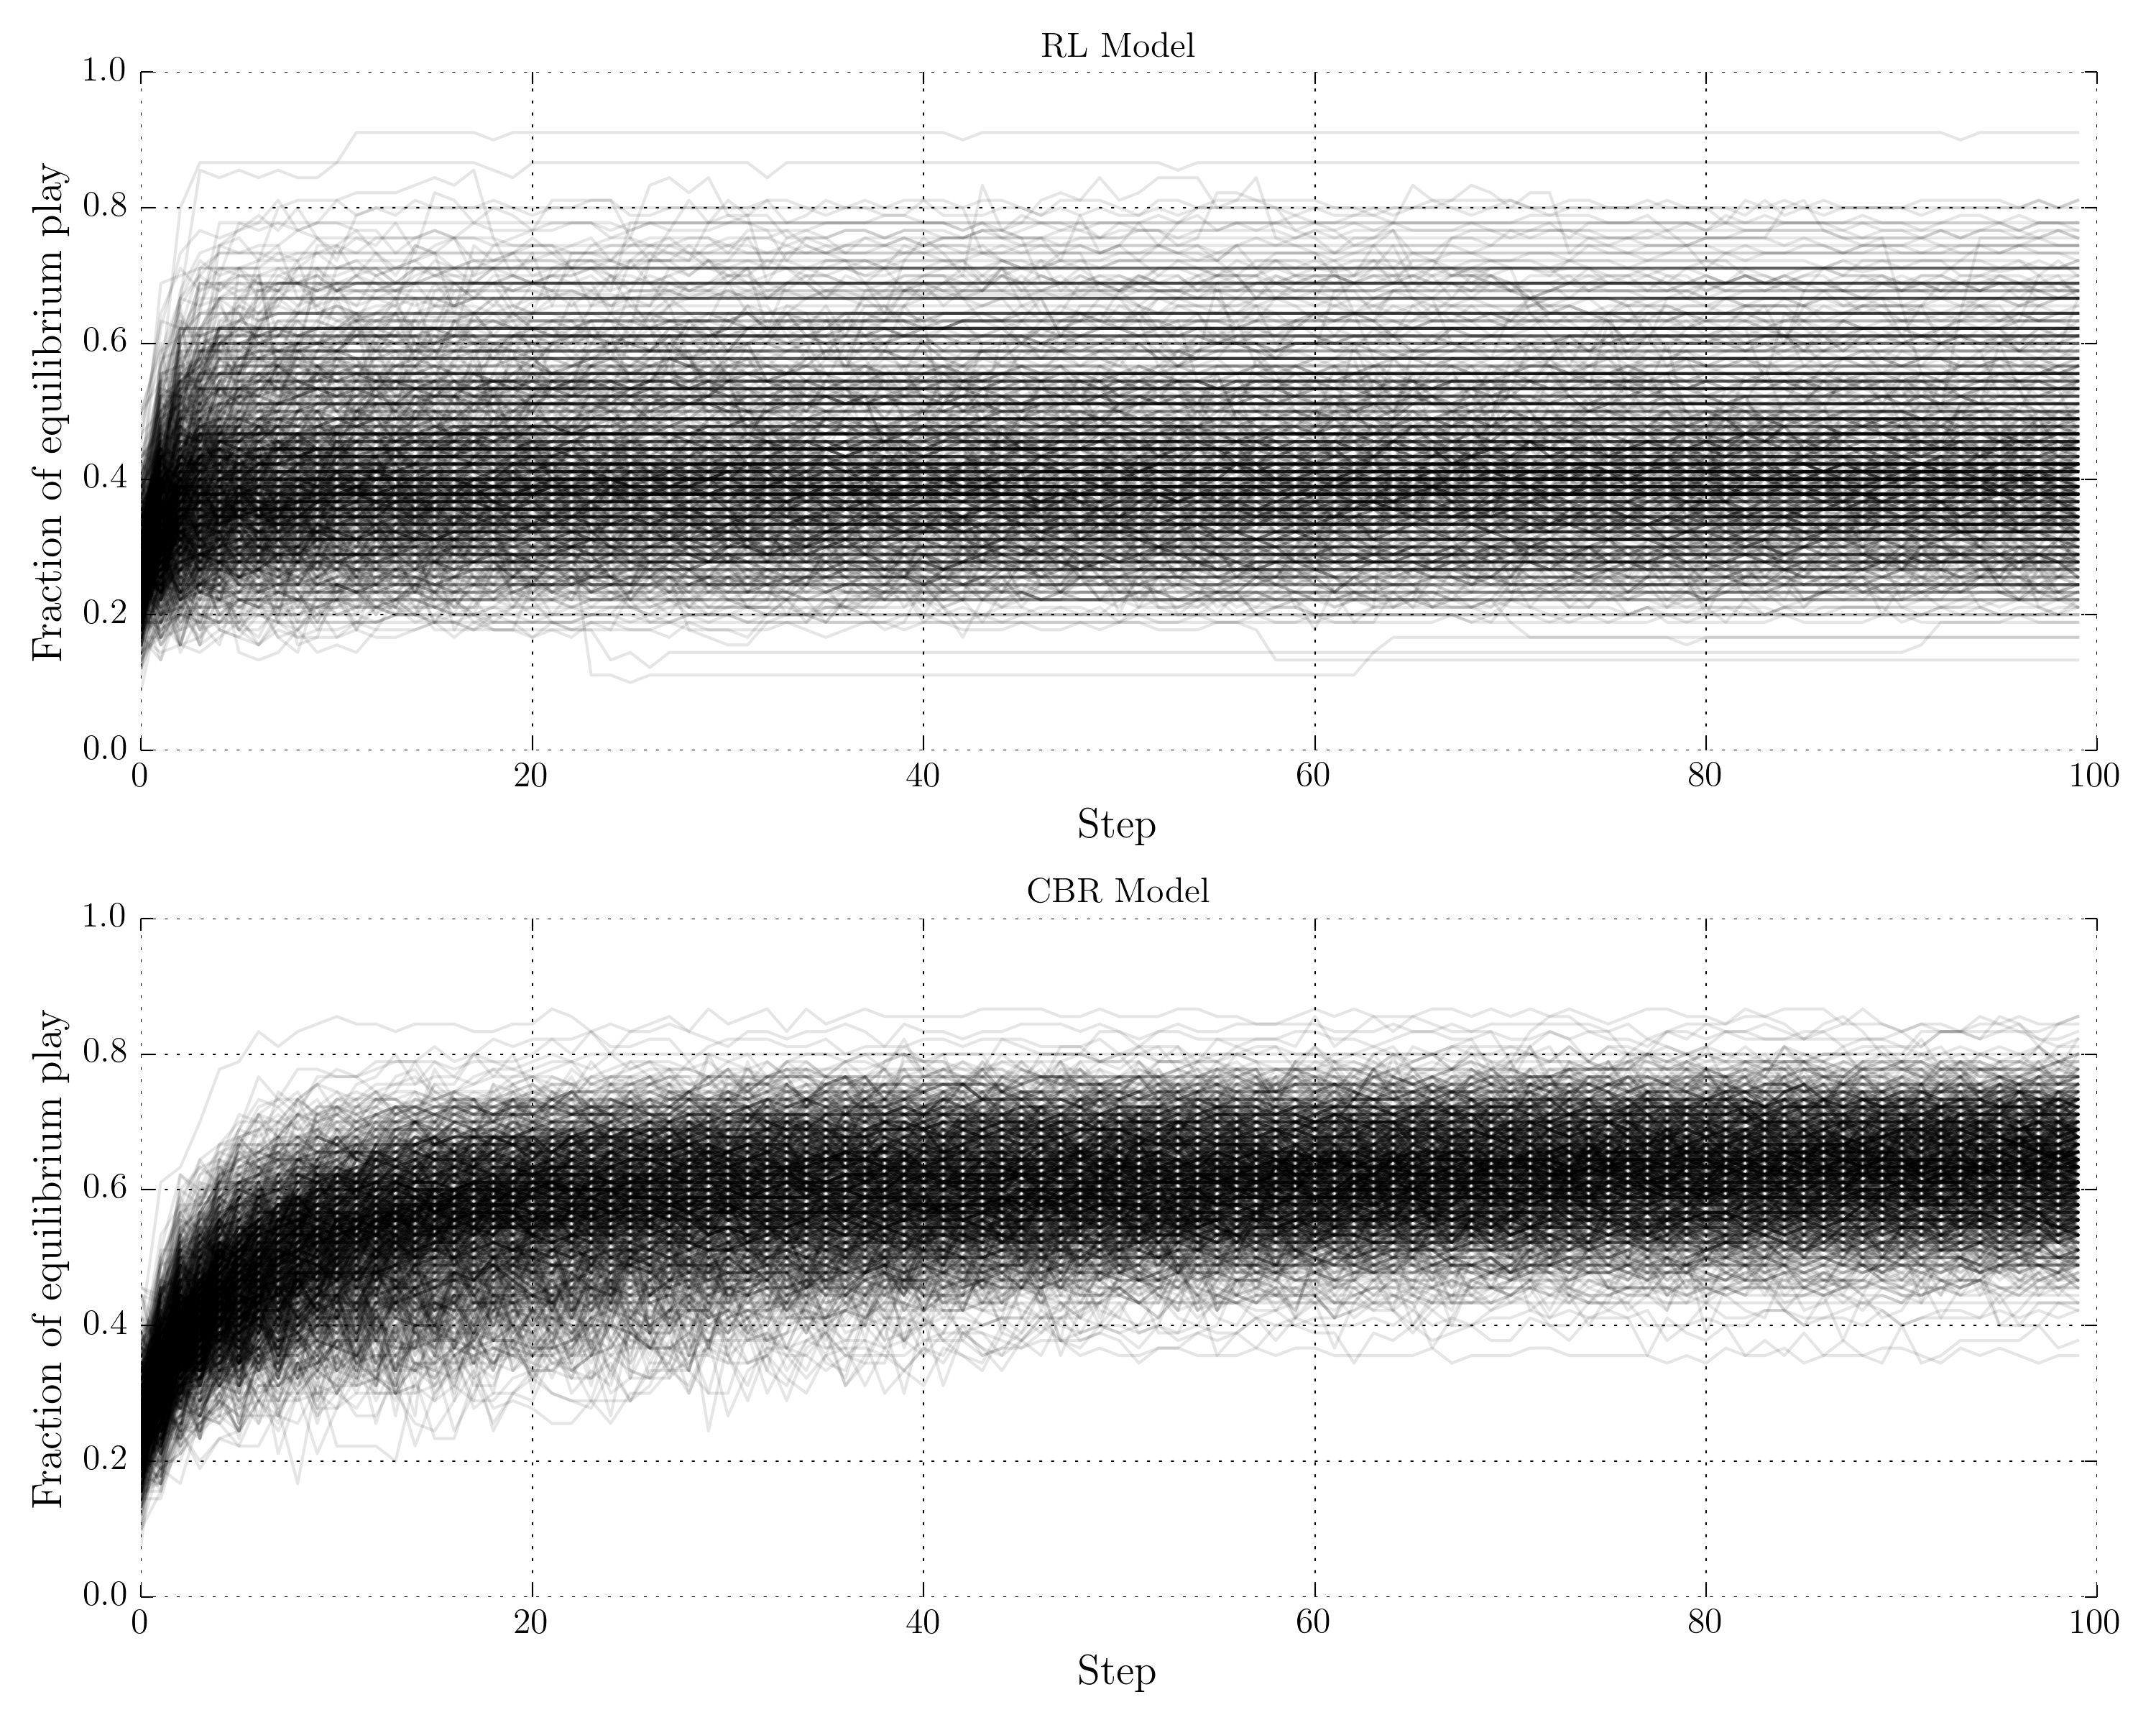
\includegraphics[width=\textwidth]{WarReason/Figures/SC_1_traces}
    \caption{Small Crisis (Static) -- Traces}
    \label{fig:sc1_traces}
    \figSpace
\end{figure}

\begin{figure}[h!]
	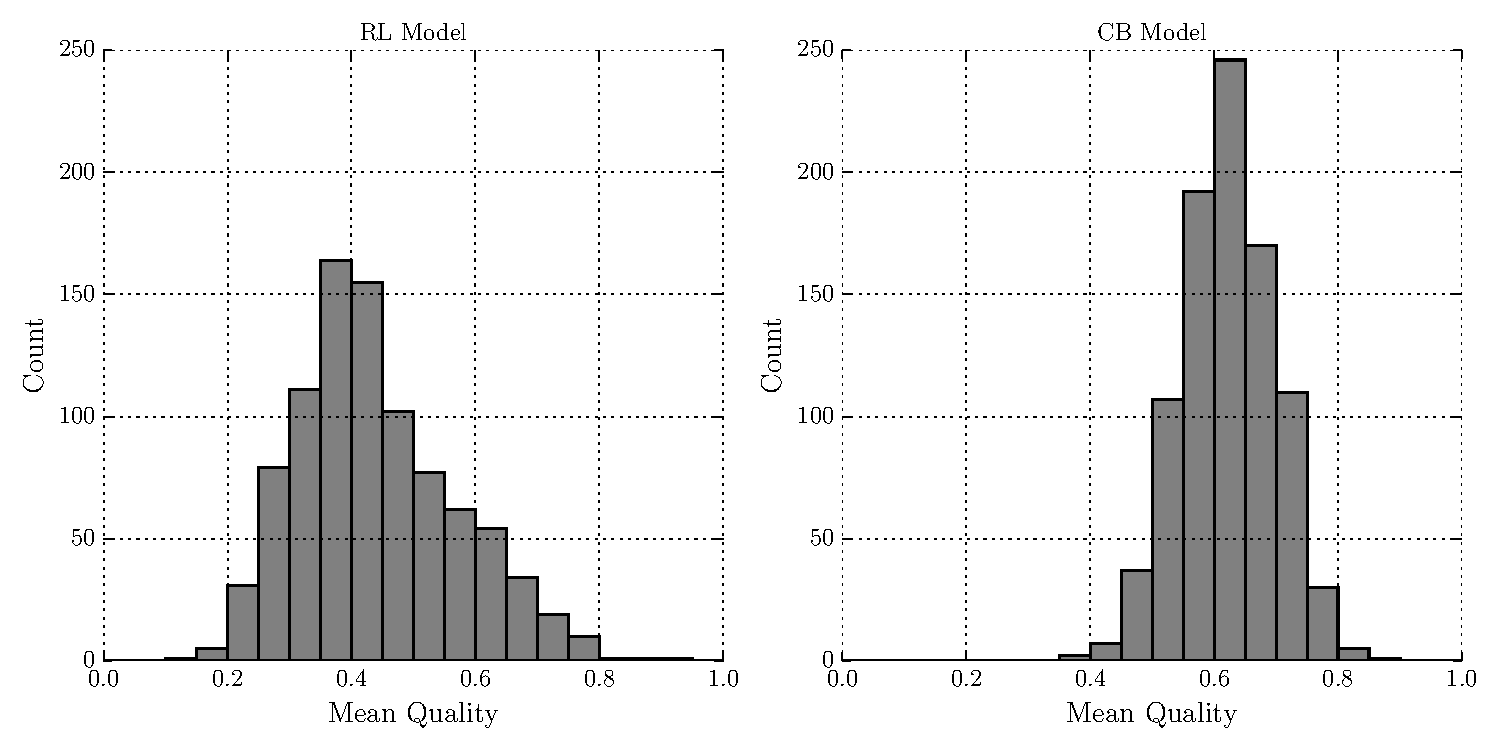
\includegraphics[width=\textwidth]{WarReason/Figures/SC_1_histograms}
    \caption{Small Crisis (Static) -- Quality Distribution}
    \label{fig:sc1_outcomes}
    \figSpace
\end{figure}

\begin{figure}[h!]
	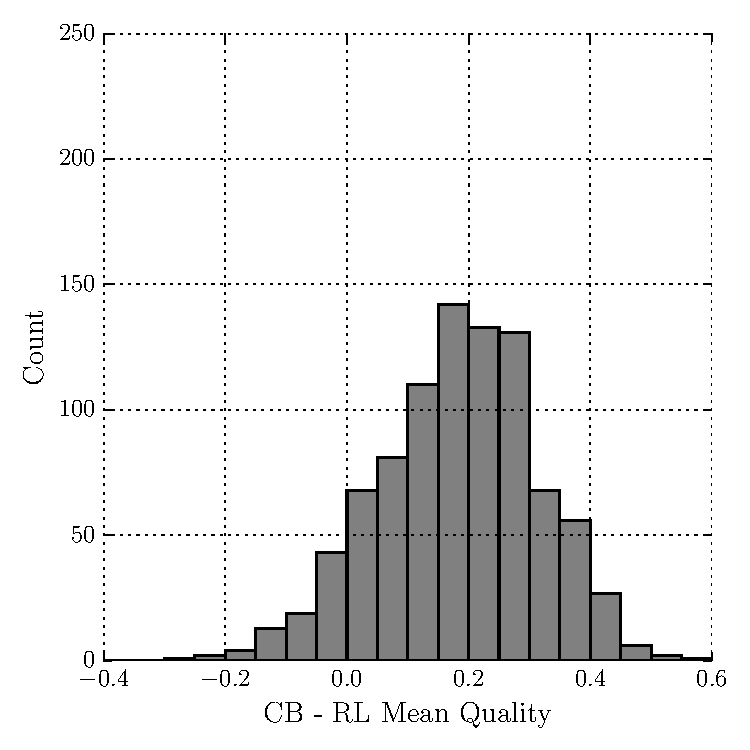
\includegraphics[width=0.5\textwidth]{WarReason/Figures/SC_1_deltas}
    \caption{Small Crisis (Static) -- CB and RL Differences}
    \label{fig:sc1_deltas}
    \figSpace
\end{figure}


Initially, let us examine the Static variant runs. Figure \ref{fig:sc1_traces} shows the traces of the equilibrium frequency at each step across all the model runs, for both agent types. For the pure RL agents, we see a variety of behaviors emerging: in some cases, the models rapidly converge to near-equilibrium behavior, while in others appear to converge to a behaviors further away from equilibrium than we would expect solely due to chance. Figure \ref{fig:sc1_outcomes} shows the distributions of the run qualities (mean fraction of interactions where the outcome matches the equilibrium) across the different runs. We immediately see that both distributions are skew normal. The CB model produces better (more consistently closer to equilibrium) behavior: its mean is greater, while its standard deviation and skew are both smaller. This is in line with my earlier hypothesis in Section \ref{decisionmaking_models}, and implies that the CB model provides agents with more strategic behavior.

Since each model instantiation is run twice with the same seed, once with RL agents and once with CB agents, we can directly compare the equilibrium frequency for each seed and find the difference between the CB and RL mean equilibrium frequencies for each. The distribution of the differences is shown in Figure \ref{fig:sc1_deltas}. This distribution is also approximately skew normal, with a mean of 0.18 ($p$-value indistinguishable from 0). This allows us to conclude that the case-based reasoning decisionmaking model produces behavior which is robustly better than the pure reinforcement learners when controlling for other factors -- exactly as we would expect.
%% RAX: Normality test?

\begin{figure}[h!]
	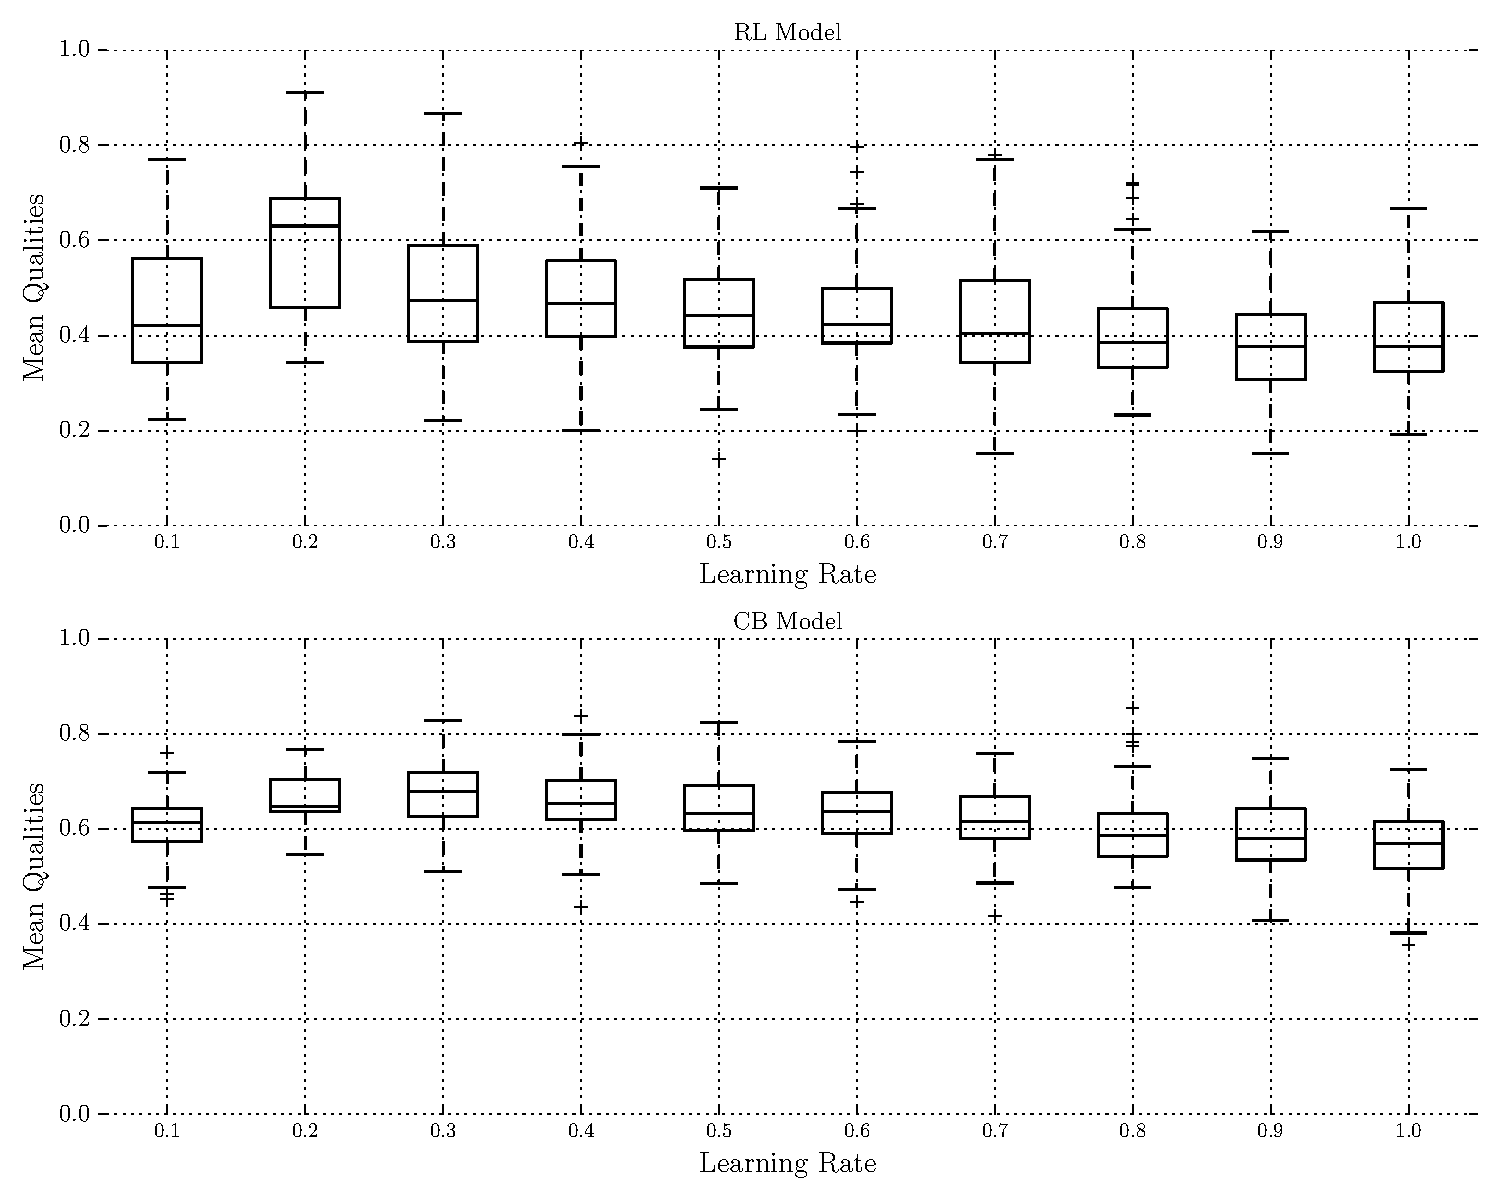
\includegraphics[width=\textwidth]{WarReason/Figures/SC_1_boxwhiskers}
    \caption{Small Crisis (Static) -- Quality by Learning Rate}
    \label{fig:sc1_boxwhiskers}
    \figSpace
\end{figure}

Another important question is whether different learning parameters yield substantially different behaviors. Figure \ref{fig:sc1_boxwhiskers} shows box-and-whiskers plots comparing the distribution of run qualities for each learning rate parameter. Overall, the differences are small, though statistically significant (with one- and two-way ANOVA tests yielding $p$-values indistinguishable from zero). Linear models of run quality to learning rate place a negative coefficient on the learning rate, indicating that lower learning rates tend to lead to higher expected qualities\footnote{Note, however, that there is a discontinuity at $\alpha=0$ where the initial weights would never change, meaning that all decisions will be made with equal probability.}. In other words, agents learn best when adjusting their behavior relatively slowly and placing most of the weight on the total of their past experiences rather than each new one -- again, an intuitive but satisfying result. Visual examination of the results in Figure \ref{fig:sc1_boxwhiskers} suggests that performance does not have a simple linear relationship with learning rate, and that both decisionmaking models have an optimal learning rate, which are different for each. The median quality for the RL model where the learning rate is 0.2 is substantially higher than the maximum of the inter-quartile range (the box) for the rest of the values, indicating that the maximum performance is attained somewhere near $\alpha \approx 0.2$. There is no similar obvious optimal learning rate for the CB model; a learning rate of 0.3 produces the highest median quality, but the distributions produced by values between 0.3 and 0.5 are essentially indistinguishable from one another, though higher than the distributions produced at the extreme values.
% RAX: Can we compare to other models w/ adjustable learning constants?

Even the best-performing model runs do not result in equilibrium play on all interactions; in general, the majority of model instantiations see equilibrium outcomes on the order of half the interactions. However, as we will discuss in more detail below, the majority of historic real-world interactions do not result in the equilibrium either. Suppose that the decisionmaking process of the model agents were an unknown black box, as real states' decisionmaking processes are. We could propose the game-theoretic equilibrium as a model of the agent decisionmaking, and test whether the equilibrium outcome is a useful predictor of the interaction outcomes. Following the methodology of \citet{bennett_2000}, I use logistic regressions to test whether the equilibrium is indeed a good predictor of observed outcomes.

\begin{table}
	\caption{Small Crisis (Static) -- Logistic Regressions}
	\label{table:sc1_logits}
	\begin{subtable}{\textwidth}
	\begin{center}
	\caption{RL Model}
	\begin{tabular}{lccccc}
		\hline
		            & StatusQuo & Capitulate1 & Capitulate2 &   War1   &   War2     \\
		\hline
		Capitulate1 & -0.04***  & 2.73***     & 0.76***     & -1.49*** & 1.19***    \\
		            & (0.00)    & (0.01)      & (0.01)      & (0.01)   & (0.01)     \\
		Capitulate2 & -0.42***  & 1.79***     & 1.43***     & -0.93*** & -0.99***   \\
		            & (0.00)    & (0.01)      & (0.00)      & (0.01)   & (0.02)     \\
		War1        & -0.08***  & -0.52***    & -0.41***    & 0.13***  & 1.30***    \\
		            & (0.00)    & (0.02)      & (0.00)      & (0.00)   & (0.01)     \\
		Const.      & 1.05***   & -5.63***    & -2.55***    & -1.55*** & -4.79***   \\
		            & (0.00)    & (0.01)      & (0.00)      & (0.00)   & (0.01)     \\
		\hline
		\hline
		\multicolumn{6}{l}{Standard errors in parentheses.} \\
		\multicolumn{6}{l}{* $p<.1$, ** $p<.05$, *** $p<.01$} \\
		\end{tabular}
		\end{center}
		%\label{table:sc1_logits}
		\tableSpace
	\end{subtable}


	\begin{subtable}{\textwidth}
		\begin{center}
		\caption{CB Model}
		\begin{tabular}{lccccc}
					&			&			  &				&		   &           \\
		\hline
		            & StatusQuo & Capitulate1 & Capitulate2 &   War1   &   War2     \\
		\hline
		Capitulate1 & -0.44***  & 4.28***     & 0.70***     & -1.36*** & 1.88***    \\
		            & (0.00)    & (0.01)      & (0.01)      & (0.01)   & (0.01)     \\
		Capitulate2 & -1.08***  & 0.70***     & 3.51***     & -1.98*** & -3.09***   \\
		            & (0.00)    & (0.02)      & (0.00)      & (0.01)   & (0.07)     \\
		War1        & -1.74***  & 0.46***     & -0.36***    & 1.67***  & 0.96***    \\
		            & (0.00)    & (0.01)      & (0.01)      & (0.00)   & (0.01)     \\
		Const.      & 0.48***   & -5.35***    & -3.23***    & -0.70*** & -4.89***   \\
		            & (0.00)    & (0.01)      & (0.00)      & (0.00)   & (0.01)     \\

		\hline
		\hline
		\multicolumn{6}{l}{Standard errors in parentheses.} \\
		\multicolumn{6}{l}{* $p<.1$, ** $p<.05$, *** $p<.01$} \\
		\end{tabular}
		\end{center}
		%\label{table:sc1_logits}
	\end{subtable}
\tableSpace
\end{table}

\begin{figure}[h!]
	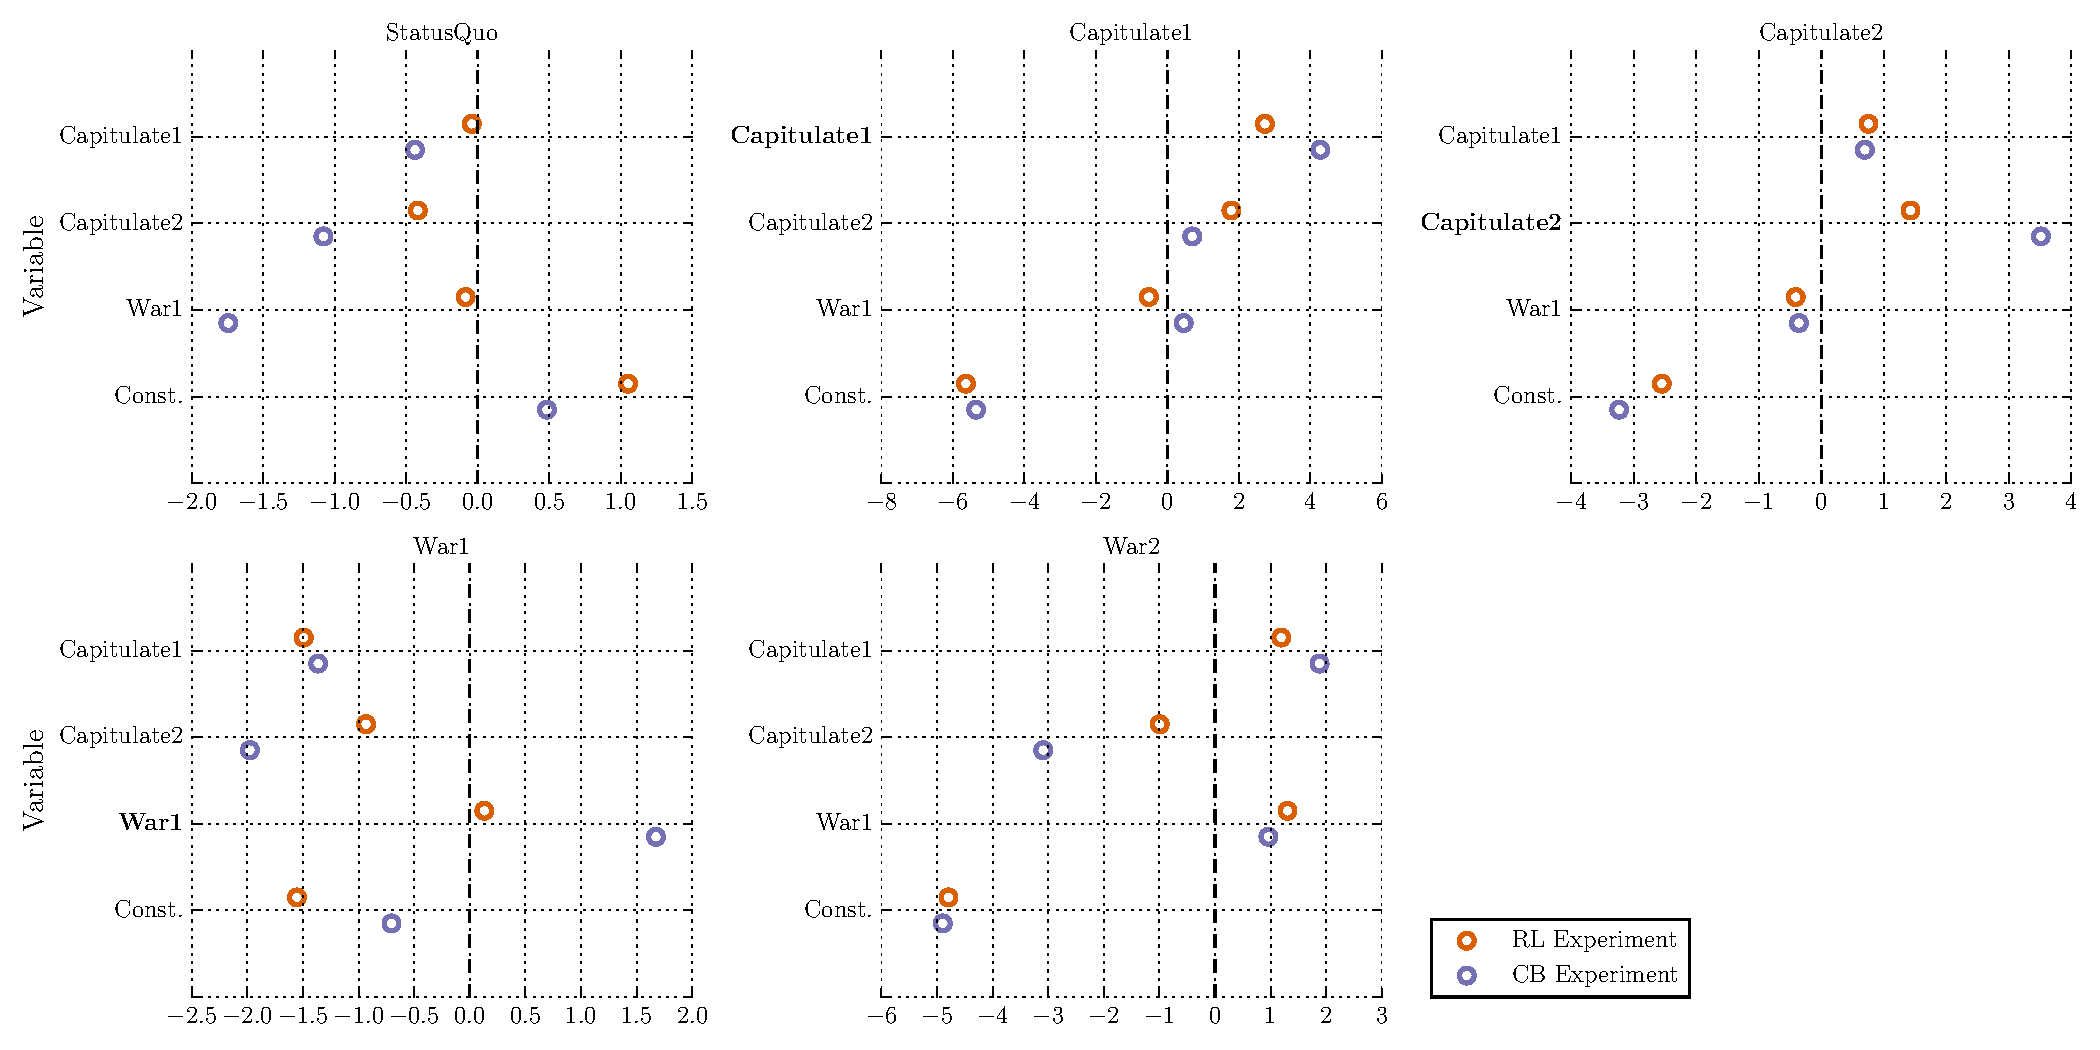
\includegraphics[width=0.95\textwidth]{WarReason/Figures/SC1_Coeffs}
    \caption{Small Crisis (Static) -- Logistic Regression Coefficient Plots}
    \label{fig:sc1_coeffs}
    \figSpace
\end{figure}

The results of these regressions are reported in Table \ref{table:sc1_logits}, and shown visually in Figure \ref{fig:sc1_coeffs}. In line with the results of \citet{bennett_2000}, across both decisionmaking models, the equilibrium is a strong predictor of a corresponding observed outcome, while other equilibria have smaller, often negative, coefficients. This effect is consistently more powerful for the CB model, with larger equilibrium coefficients and smaller coefficients on other variables for each regression. In other words, when the agents are using case-based learning, the equilibria is a stronger predictor of their actual behavior than when the agents are using simple reinforcement learning. This is in line with the hypothesis that the CB agents will behave more rationally than the RL agents. Furthermore, outcomes closer to the equilibrium in the game tree are stronger predictors than further outcomes, suggesting that the agents are playing sequences of moves that are close to the equilibria sequences, deviating only in the step.  
% Last point seems important -- expand?

\begin{figure}[h!]
	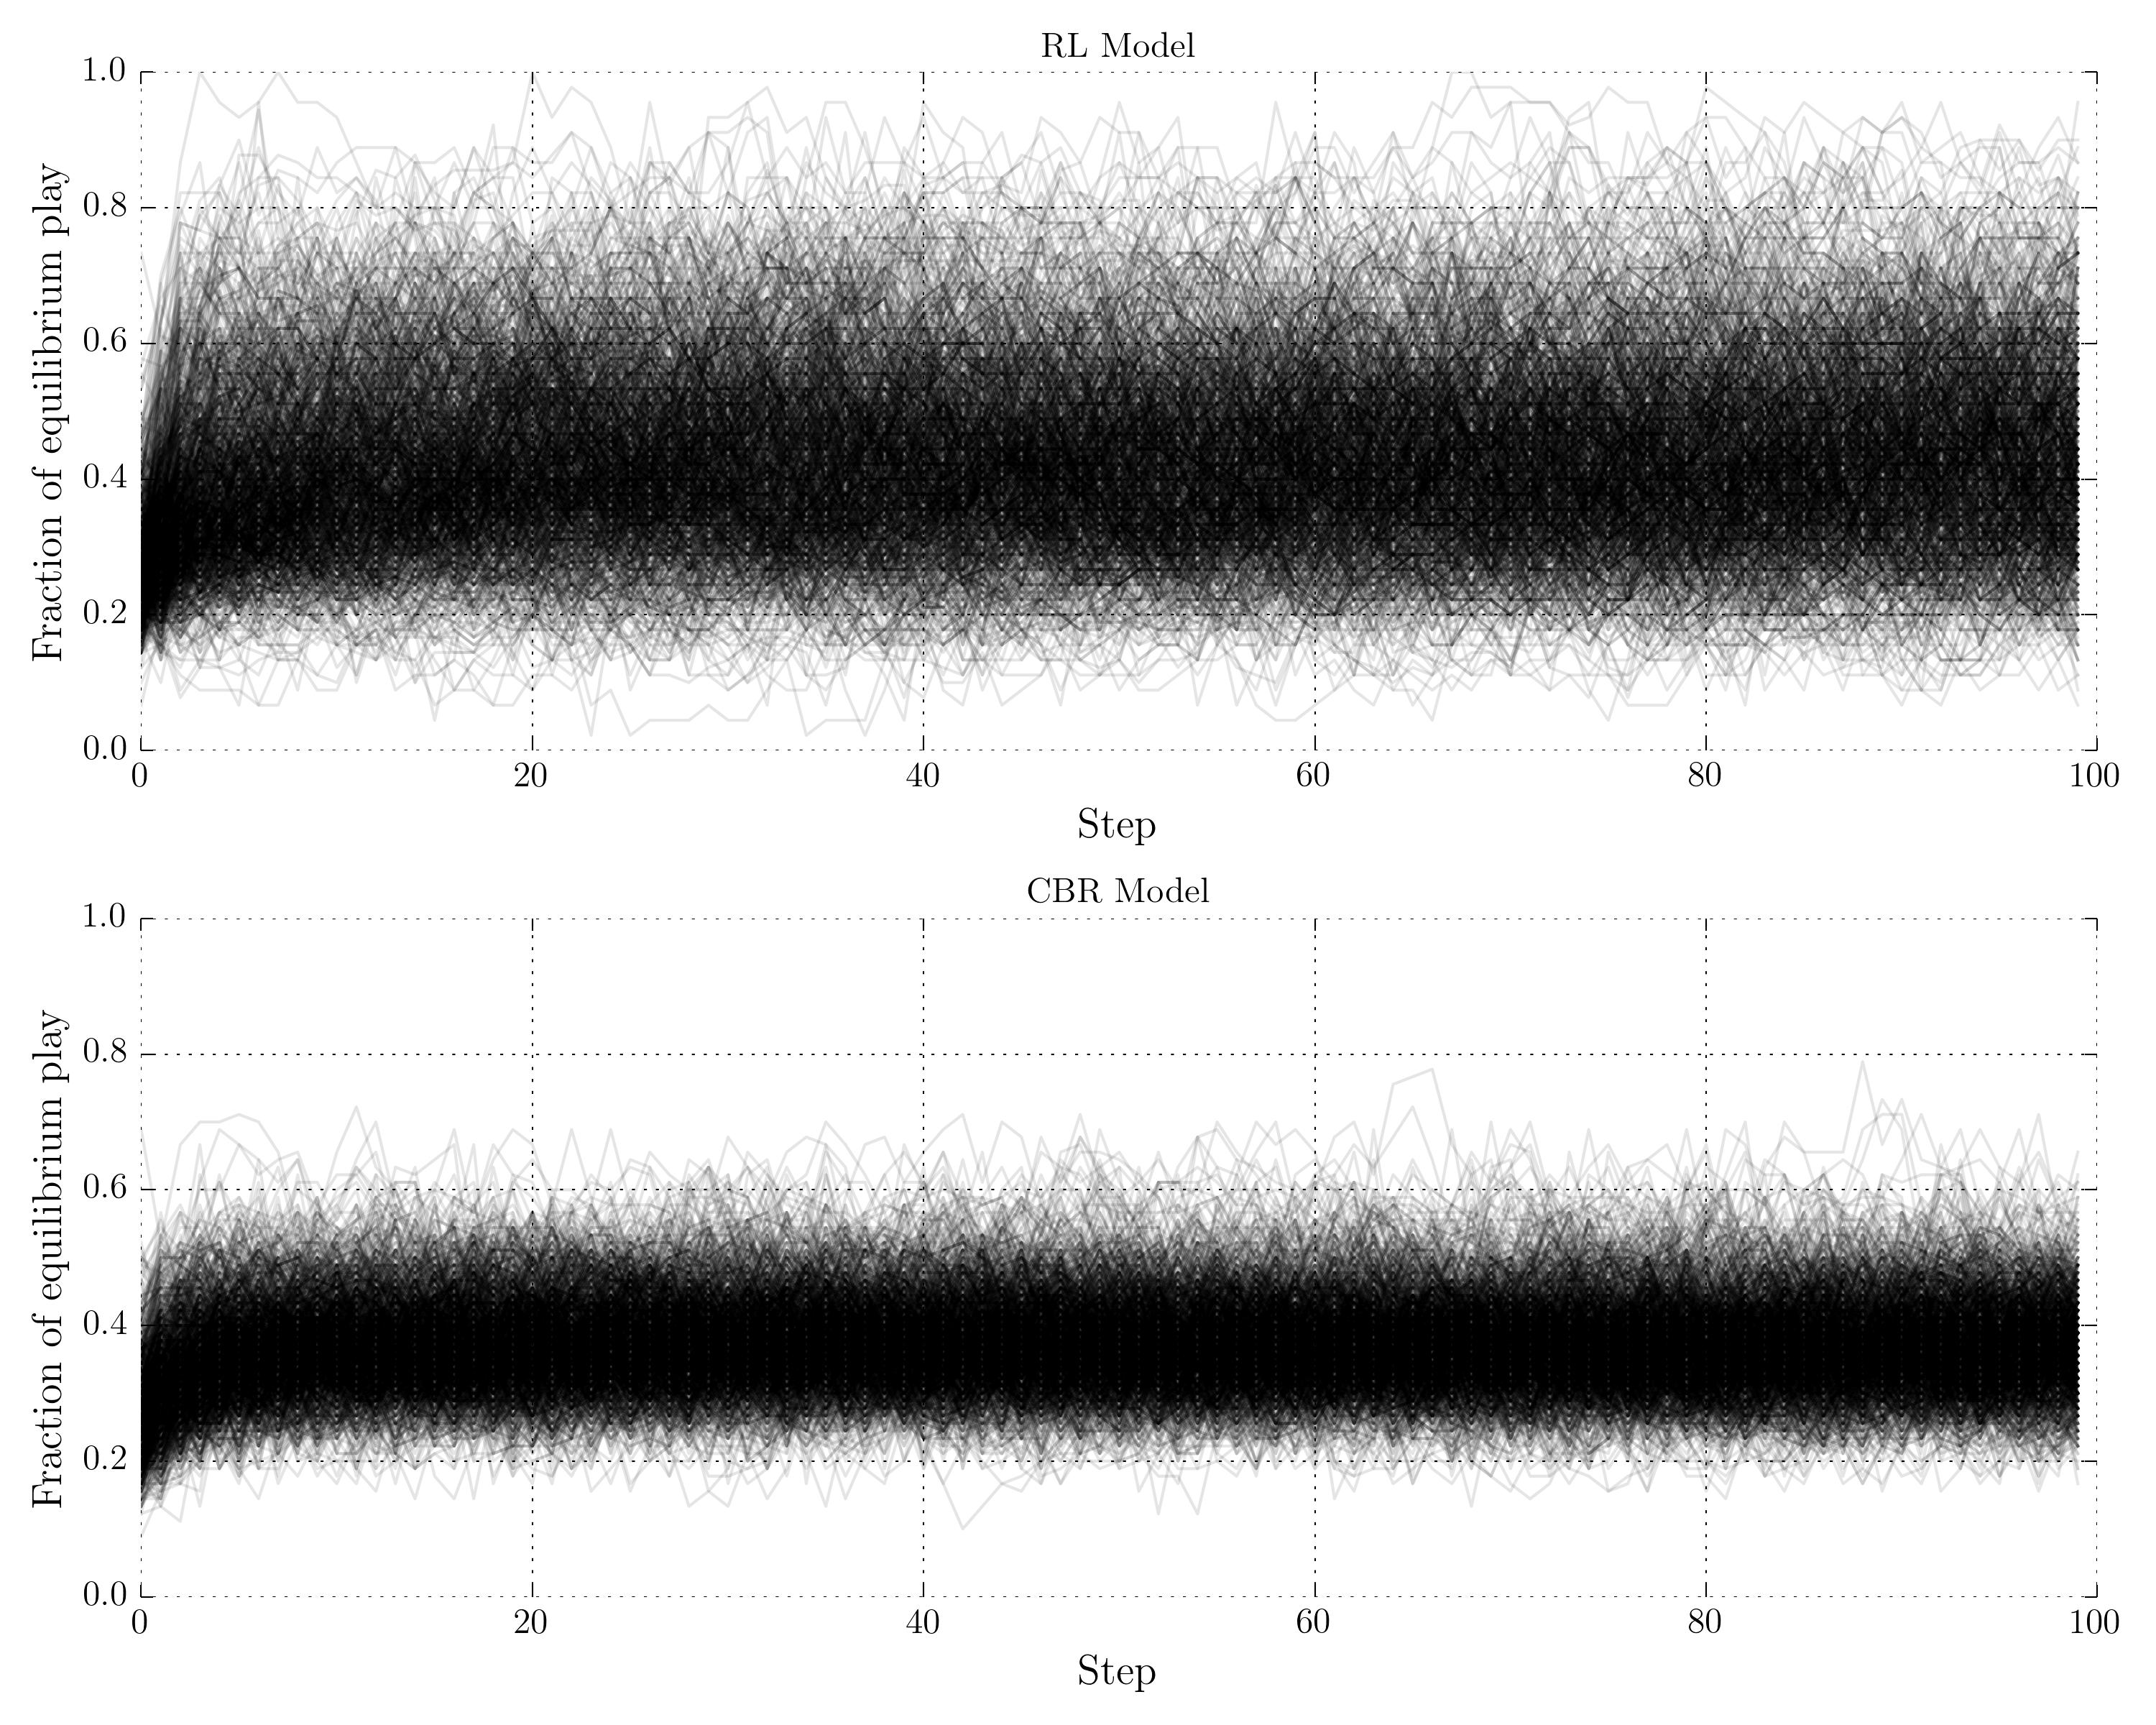
\includegraphics[width=\textwidth]{WarReason/Figures/SC_2_traces}
    \caption{Small Crisis (Dynamic) -- Traces}
    \label{fig:sc2_traces}
    \figSpace
\end{figure}

\begin{figure}[h!]
	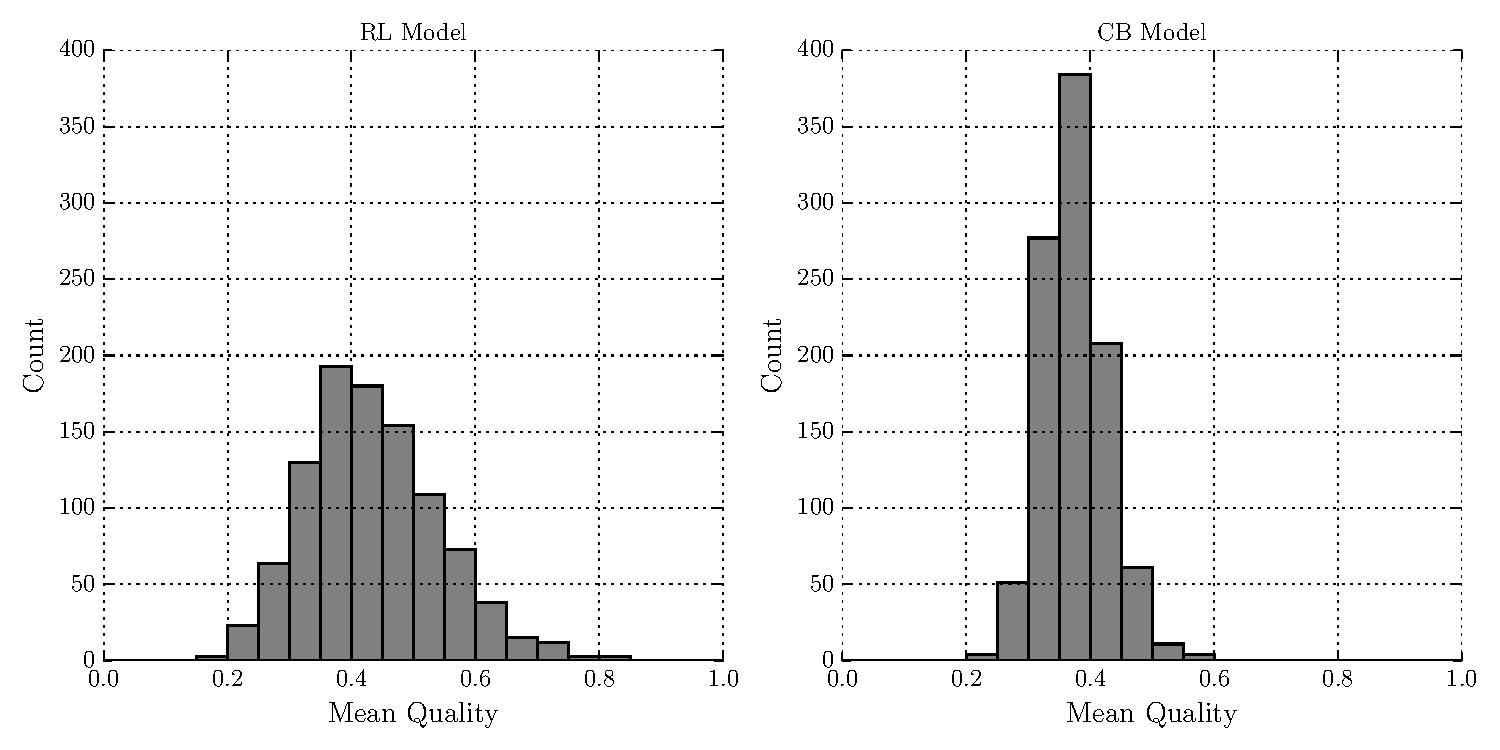
\includegraphics[width=\textwidth]{WarReason/Figures/SC_2_histograms}
    \caption{Small Crisis (Dynamic) -- Quality Distribution}
    \label{fig:sc2_outcomes}
    \figSpace
\end{figure}

\begin{figure}[h!]
	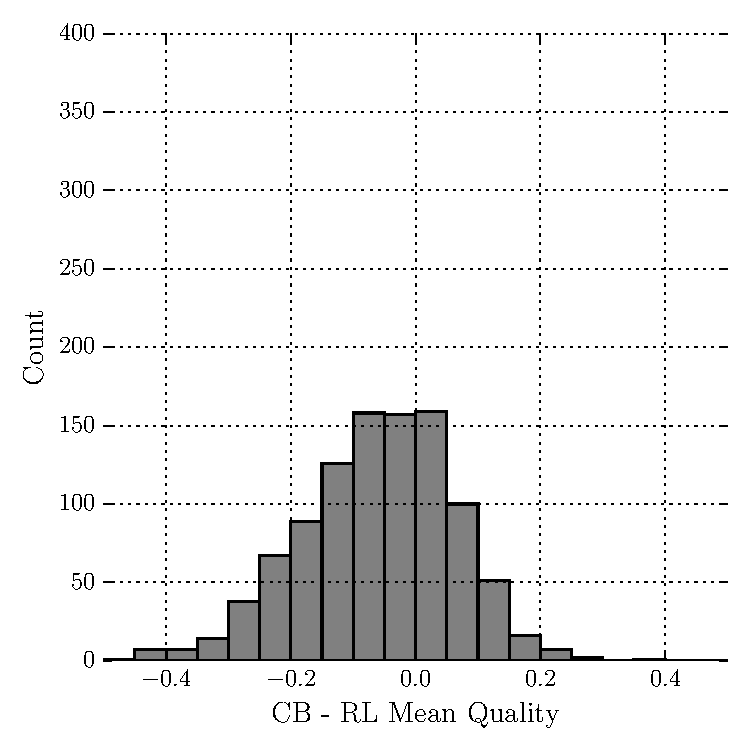
\includegraphics[width=0.5\textwidth]{WarReason/Figures/SC_2_deltas}
    \caption{Small Crisis (Dynamic) -- CB and RL Differences}
    \label{fig:sc2_deltas}
    \figSpace
\end{figure}

\subsubsection{Dynamic Variant}

Next, I repeat the above experiment and analyses with the dynamic model variant, where agent properties change from step to step. Figures \ref{fig:sc2_traces} and \ref{fig:sc2_outcomes} show the traces and distribution of outcomes, respectively. We can immediately see that overall the agents are less likely to play the equilibrium outcome compared to the Static variant, across both decisionmaking models. This is exactly in line with our intuitive expectation -- since each dyad of agents do not have a fixed set of moves to reach equilibrium, and indeed the mix of equilibrium moves across the entire population is changing, the lessons of previous interactions will be less applicable to future ones, making moves based on the learned weights less likely to result in equilibrium. Examination of the outcomes across different learning rates, as shown in Figure \ref{fig:sc2_boxwhiskers} suggests that they do not yield significant differences. This, in turn, suggests that the speed at which agents adjust their behaviors does not substantially affect the behavior the model converges to.
% Build those expectations earlier so we know what 'in line with' them means.
\begin{figure}[h!]
	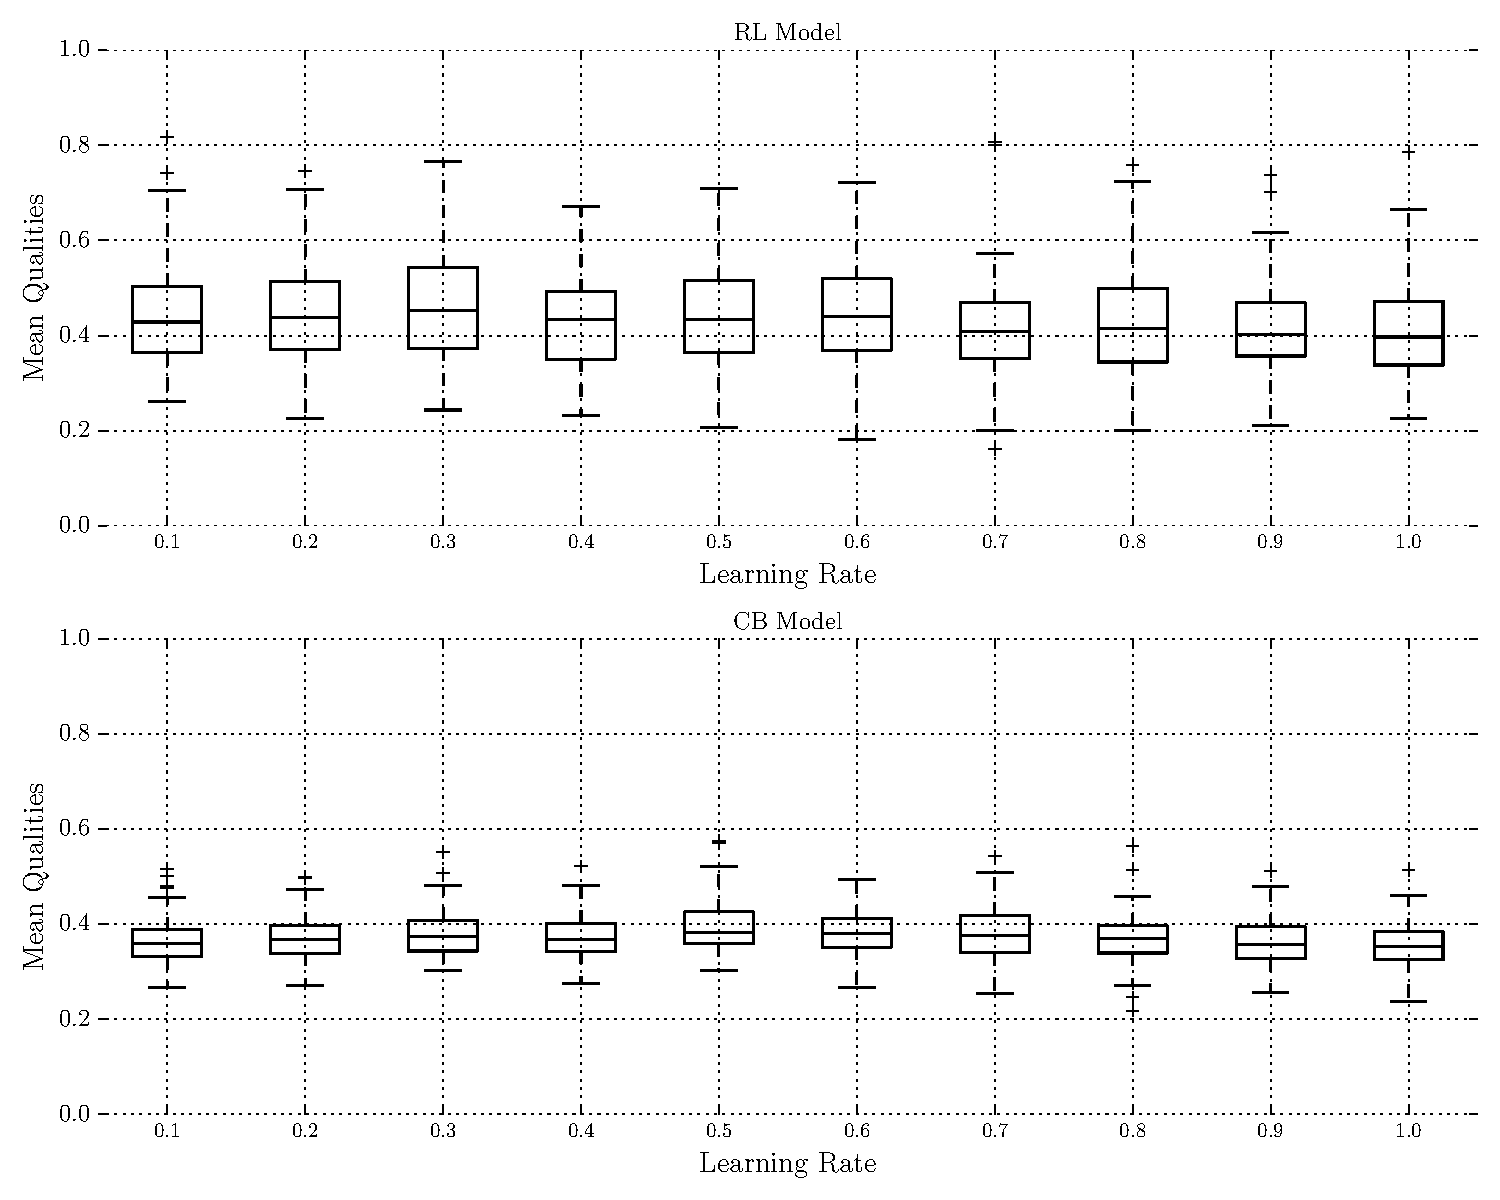
\includegraphics[width=\textwidth]{WarReason/Figures/SC_2_boxwhiskers}
    \caption{Small Crisis (Dynamic) -- Quality by Learning Rate}
    \label{fig:sc2_boxwhiskers}
    \figSpace
\end{figure}

\begin{table}[h!]

	\caption{Small Crisis (Dynamic) -- Logistic Regressions}
	\label{table:sc2_logits}

	\begin{subtable}{\textwidth}
	\begin{center}
		\caption{RL Model}
		%\label{table:sc1_logits}
	\begin{tabular}{lccccc}
		\hline
		            & StatusQuo & Capitulate1 & Capitulate2 &   War1   &   War2     \\
		\hline
		Capitulate1 & -0.13***  & 2.13***     & 0.47***     & -0.51*** & 1.30***   \\
		            & (0.01)    & (0.02)      & (0.01)      & (0.01)   & (0.02)    \\
		Capitulate2 & -0.58***  & 1.39***     & 1.47***     & 0.02***  & -0.35***  \\
		            & (0.00)    & (0.02)      & (0.01)      & (0.01)   & (0.03)    \\
		War1        & -0.24***  & -2.17***    & -0.21***    & 0.42***  & -2.46***  \\
		            & (0.00)    & (0.08)      & (0.01)      & (0.01)   & (0.07)    \\
		War2        & 0.51***   & 0.72***     & -0.65***    & -0.95*** & 1.32***   \\
		            & (0.01)    & (0.03)      & (0.01)      & (0.01)   & (0.02)    \\
		Const.      & 2.49***   & -6.33***    & -4.18***    & -2.82*** & -5.64***  \\
		            & (0.00)    & (0.02)      & (0.01)      & (0.00)   & (0.01)    \\
		\hline
		\hline
		\multicolumn{6}{l}{Standard errors in parentheses.} \\
		\multicolumn{6}{l}{* $p<.1$, ** $p<.05$, *** $p<.01$} \\
		\end{tabular}
		\end{center}
		\tableSpace
	\end{subtable}

	\begin{subtable}{\textwidth}
		\begin{center}
			\caption{CB Model}
			%\label{table:sc1_logits}
		\begin{tabular}{lccccc}
					&			&			  &				&		   &           \\
		\hline
		            & StatusQuo & Capitulate1 & Capitulate2 &   War1   &   War2     \\
		\hline
		Capitulate1 & -0.17***  & 1.26***     & -0.57***    & -0.29*** & 0.87***   \\
		            & (0.00)    & (0.01)      & (0.01)      & (0.00)   & (0.01)    \\
		Capitulate2 & -0.37***  & 0.15***     & 1.22***     & -0.33*** & -0.17***  \\
		            & (0.00)    & (0.01)      & (0.00)      & (0.00)   & (0.01)    \\
		War1        & -0.88***  & -1.20***    & 0.92***     & 0.62***  & -0.69***  \\
		            & (0.00)    & (0.01)      & (0.00)      & (0.00)   & (0.01)    \\
		War2        & -0.49***  & 1.05***     & -1.21***    & 0.17***  & 1.16***   \\
		            & (0.00)    & (0.01)      & (0.01)      & (0.00)   & (0.00)    \\
		Const.      & 0.05***   & -3.28***    & -2.32***    & -0.77*** & -3.09***  \\
		            & (0.00)    & (0.00)      & (0.00)      & (0.00)   & (0.00)    \\
		\hline
		\hline
		\multicolumn{6}{l}{Standard errors in parentheses.} \\
		\multicolumn{6}{l}{* $p<.1$, ** $p<.05$, *** $p<.01$} \\
		\end{tabular}
		\end{center}
	\end{subtable}
	\tableSpace
\end{table}

\begin{figure}[h!]
	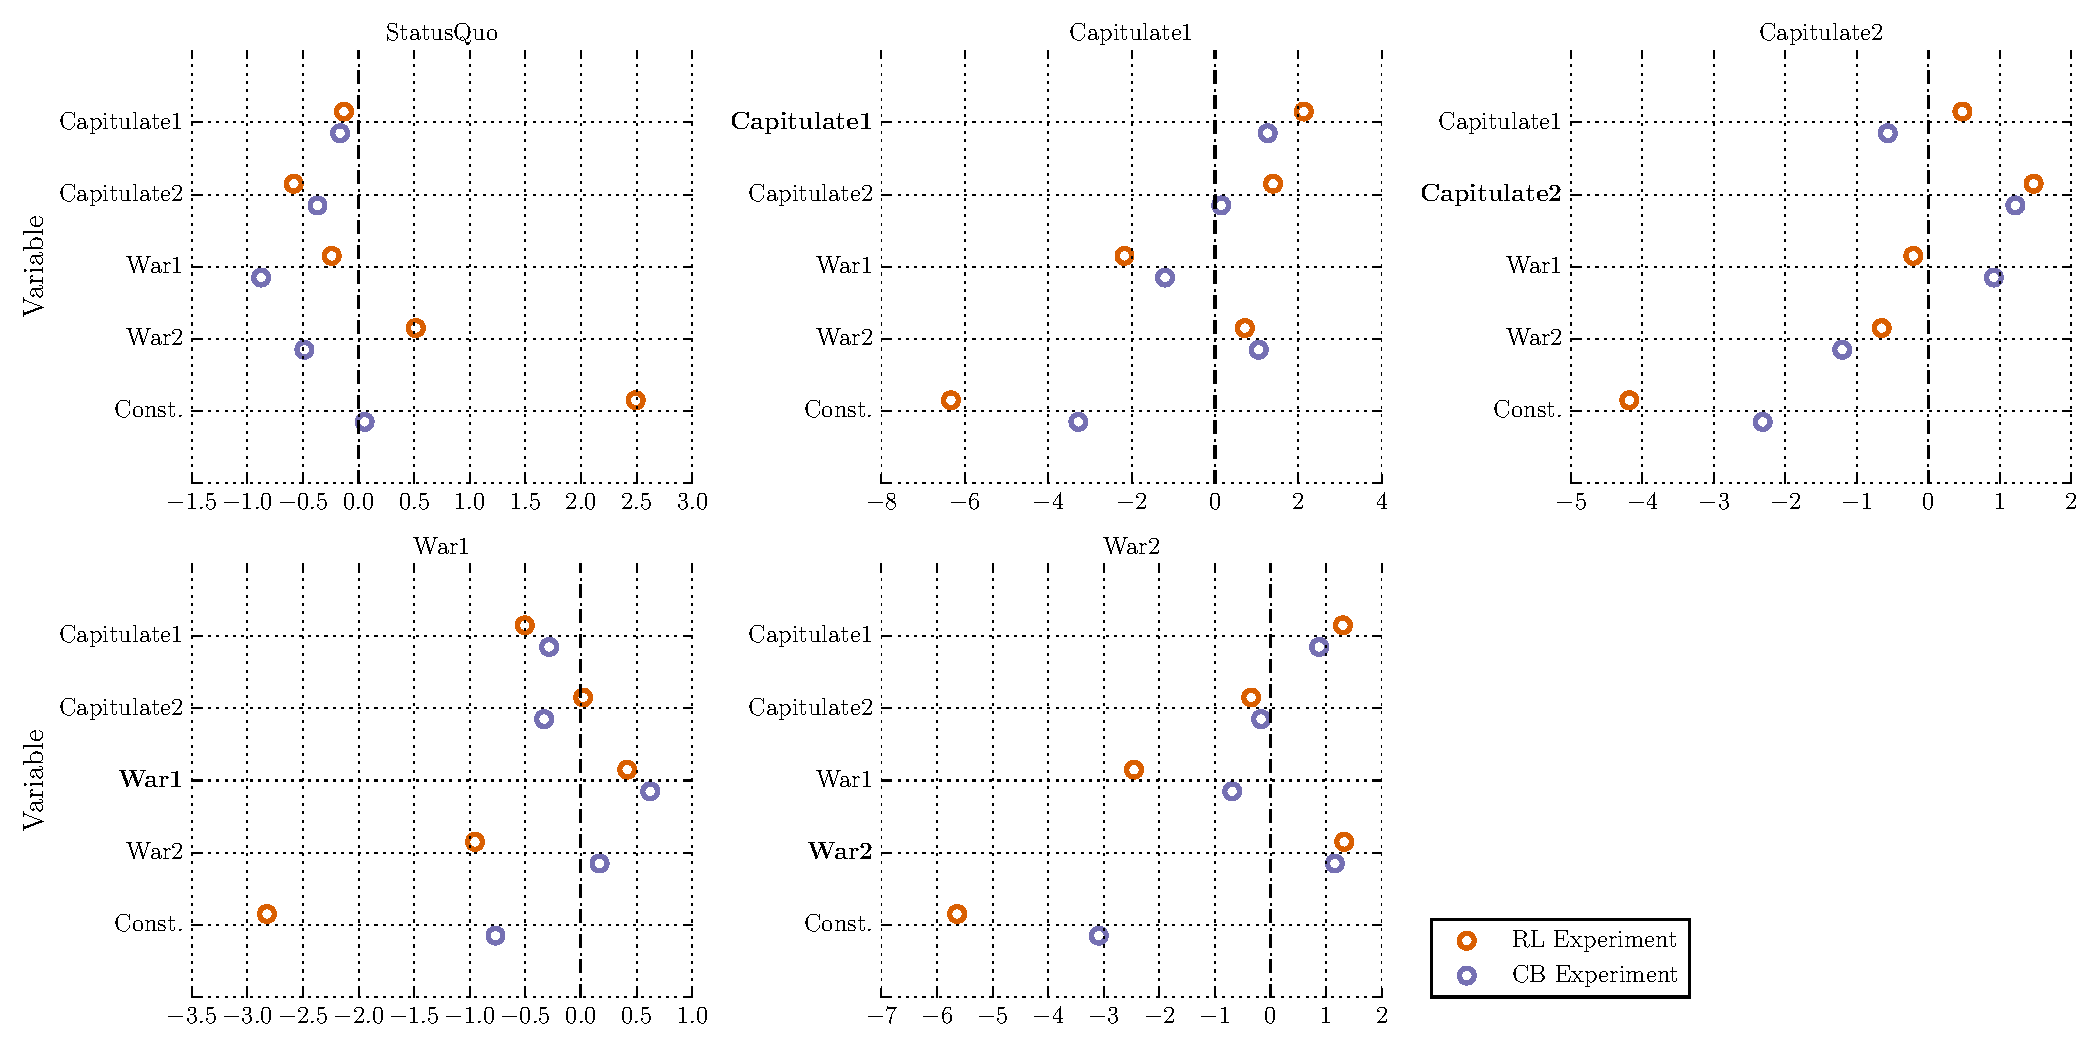
\includegraphics[width=0.95\textwidth]{WarReason/Figures/SC2_Coeffs}
    \caption{Small Crisis (Dynamic) -- Logistic Regression Coefficient Plots}
    \label{fig:sc2_coeffs}
    \figSpace
\end{figure}

A more surprising result is that the CB decisionmaking model does not outperform the RL model.  Figure \ref{fig:sc2_deltas} shows the distribution of differences between the model qualities; it has a mean of -0.06, indicating that on average the CB agents perform very slightly worse than the RL agents. This is confirmed by the logistic regressions, reported in Table \ref{table:sc2_logits} and shown visually in Figure \ref{fig:sc2_coeffs}. As with the regressions done on the Static variant results, the equilibria are still positive predictors of a corresponding outcome. Unlike with the Static variant, however, the equilibrium is not a stronger predictor of the outcome of the CB models than of the RL models. This contradicts the hypothesis that the CB decisionmaking model is broadly superior to the the RL decisionmaking model in terms of approaching rational play.

In the previous model variant, the CB agents were implicitly learning best moves against each particular agent. In this variant, since agent properties are changing, there is no single best response to be learned. Additionally, with ever-changing agent properties, there are more potential coordinates populating the case history space more densely. The equilibrium moves exhibit discontinuities across this space; however, the updating rule, whereby a new interaction updates both its own coordinate point and those of the nearest previous case, mean that moves appropriate for one equilibrium but not the other may propagate across these discontinuities -- essentially, agents consider two cases more similar than they actually are. 

\subsection{International Interaction Game} \label{iig_results}

The previous, simple model allowed me to verify that the decision models were implemented properly, with the code corresponding to the model description. More substantively, the results reported above suggest that multiple agents are capable of learning to play extensive-form games against each other in a manner approaching rational behavior, in line with my initial hypothesis. Furthermore, the difference in performance of the RL and CB models between the static and dynamic variant complicates expectations for the real world, which is itself dynamic. With these results in mind, I move from the notional, simplified international system to the full International Interaction Game (IIG) with the EUGene data, as described in Section \ref{sec:iig_description}. 

I carry out these experiments as follows. For each of the RL and CB decisionmaking models, I instantiate 105 model runs\footnote{The non-round number is due to model runs being executed in parallel on 15 cores on 16-core servers.}, with all agents utilizing the same decisionmaking model with fixed learning rates: 0.1 for the RL model, and 0.2 for the CB model. Each instantiation includes one agent for each unique country in the EUGene dataset, and is run as described in Section \ref{sec:iig_description}. I record the outcome for each interaction from each instantiation, and compare them to the equilibrium outcomes and observed events. There are thirteen possible outcomes of the extensive-form game tree, meaning that if agents were to play at random there would be a 7.7\% chance of observing an outcome equal to the equilibrium. Figure \ref{fig:ex2_traces} shows the fraction of interactions by year ending in the IIG equilibrium outcome. There are several things immediately obvious: as with the simplified model, we never see convergence to perfect equilibrium behavior. Unlike with the simplified model, however, there is not an obvious rapid initial burn-in period followed by relative stability. Instead, there is a broad range of traces showing different rates of improvement, with occasional sharp dips and upward spikes. 

\begin{figure}[h!]
    \centering

    \begin{subfigure}[t]{\textwidth}
        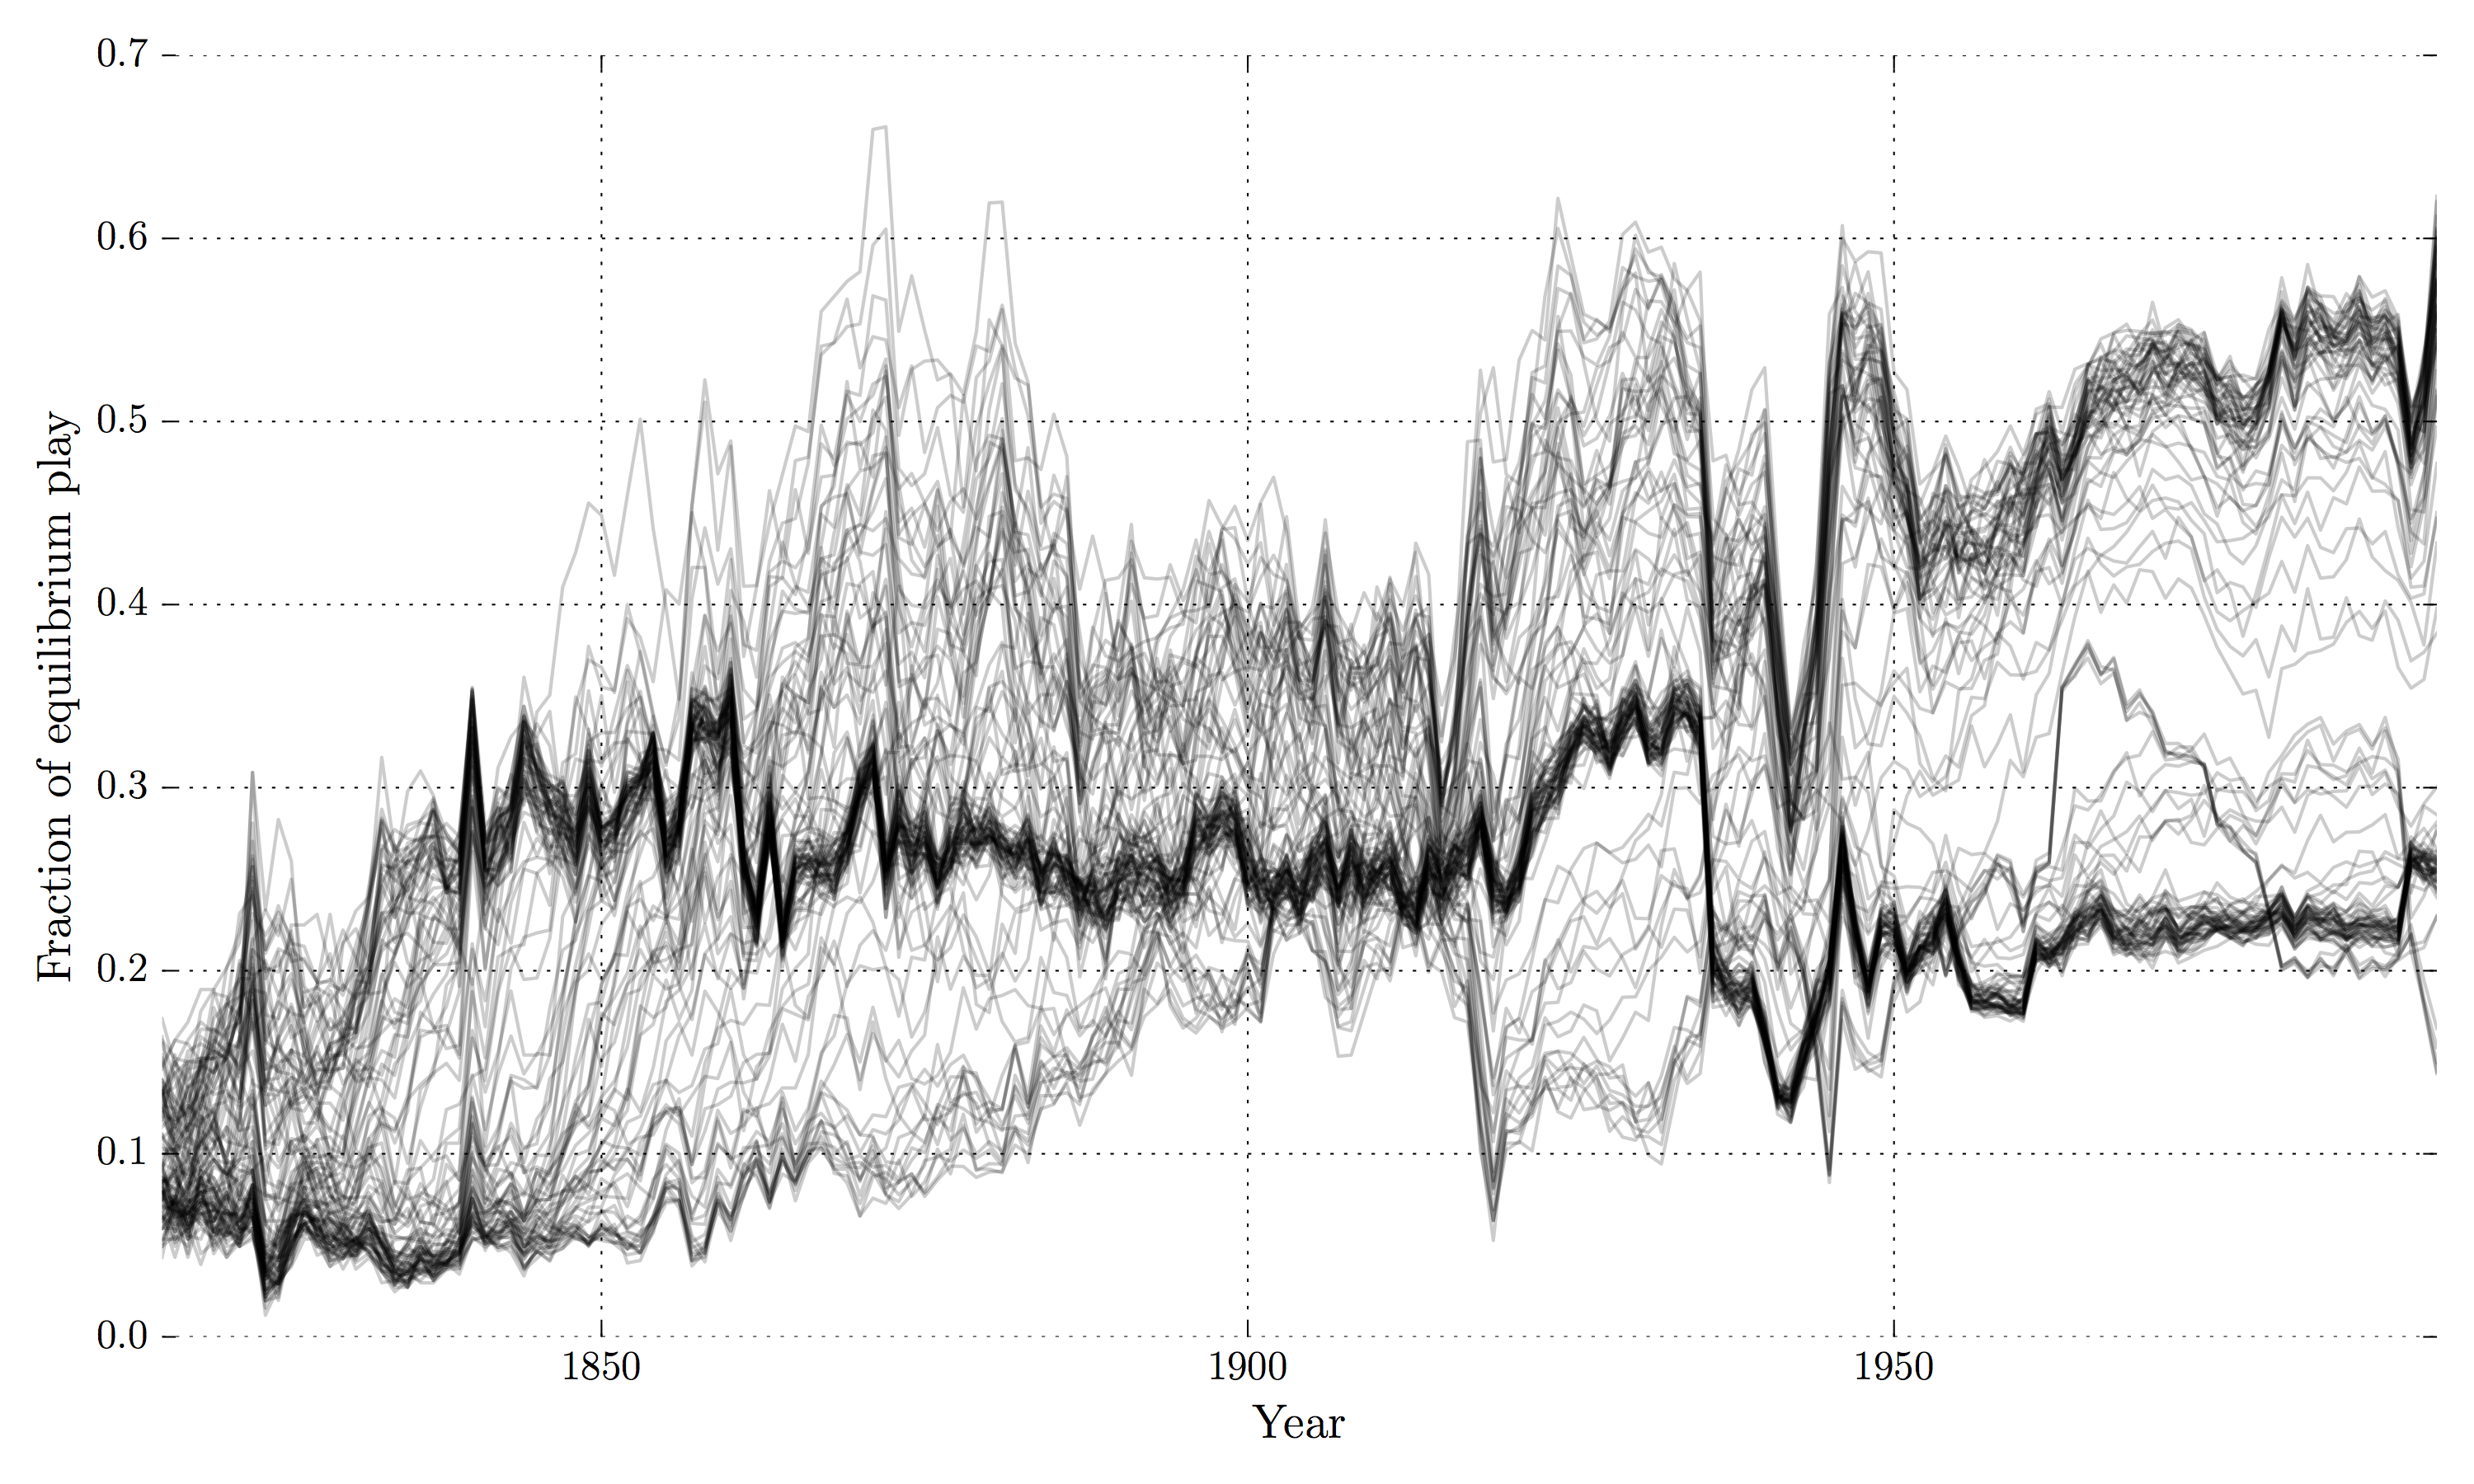
\includegraphics[width=\textwidth]{WarReason/Figures/RL_equilibria}
        \caption{Reinforcement Learning Model}
    \end{subfigure}
    
    \begin{subfigure}[t]{\textwidth}
        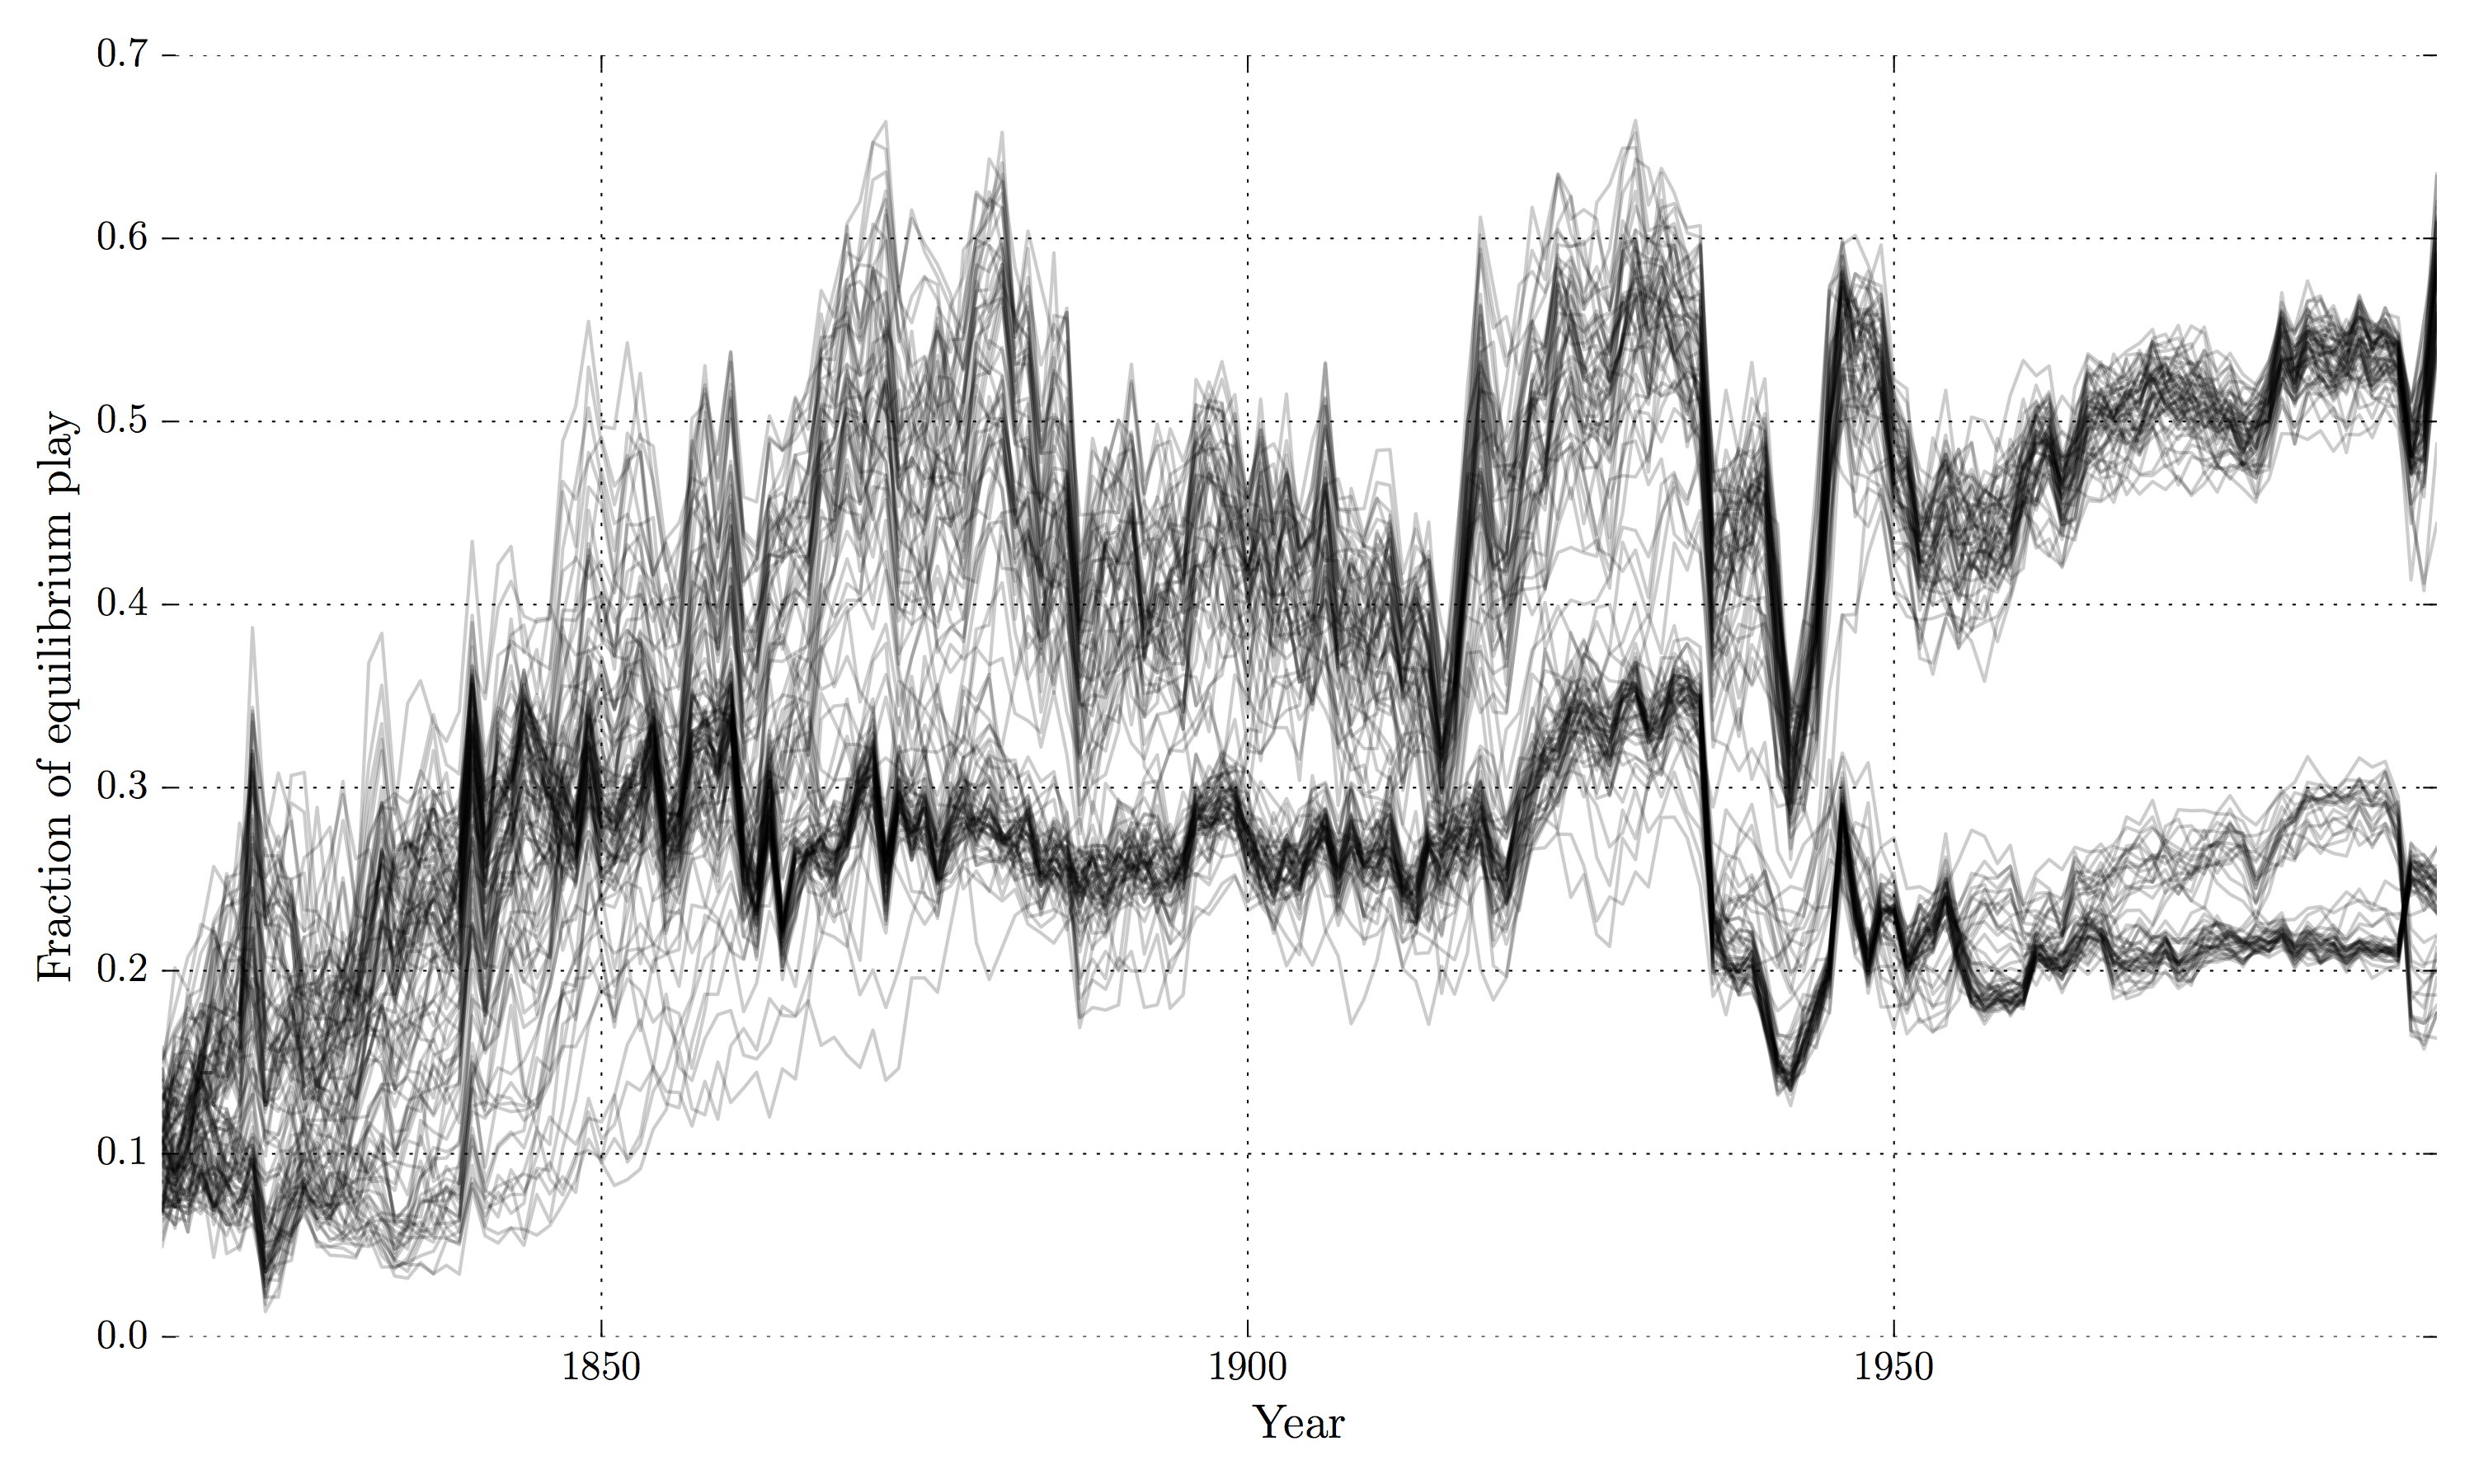
\includegraphics[width=\textwidth]{WarReason/Figures/CB_equilibria}
        \caption{Case-Based Reasoning Model}
    \end{subfigure}

    \caption{Fraction of Interactions with Equilibrium Outcome}
    \label{fig:ex2_traces}
    \figSpace
\end{figure}

It appears that the rate of improvement across the majority of CB runs is initially greater than for the RL runs; in particular, all CB runs rise above the fraction of equilibrium outcomes expected by chance earlier than the RL runs. However, there is not a clear stable performance rate reached for either decisionmaking model, with multiple substantial shifts in the rate of equilibrium play. In fact, across all the different runs, these shifts occur at similar points, in some cases in different directions. Note in particular the very obvious effects of the two world wars. Those conflicts themselves are outside the scope of the IIG and its variants: they were heavily multilateral, took place across multiple years, and radically changed the states present in the international system and alliance network between them. It appears to be the case that the shocks of the world wars substantially changes the distribution of equilibrium moves for the different agents. In some runs, this leads to a significant drop in equilibrium performance, while in others the agents either successfully rapidly adapt or have previously learned distributions of behaviors which prove to be improvements in the new environment. In contrast, following World War II, there is no similar improvement, with the majority of traces demonstrating rapid deterioration in equilibrium play. 

Across both the pure reinforcement learning and case-based reasoning decisionmaking model variants, there appear to be several overall attractors, with multiple model instantiations demonstrating similar behavior. These attractors are visible in Figure \ref{fig:ex2_traces} as the darker regions where multiple line traces come together. Both variants have one attractor with a fraction of equilibrium play at approximately 0.25, which emerges early on. Across both variants, this attractor shows a sharp falloff approximately during the 1930s, then rebounds somewhat, and stabilizes from 1950 until the end of the model timeframe. Both variants also exhibit a second attractor which emerges later, at a substantially higher equilibrium fraction. In the RL variant, the second attractor emerges most during the mid-1930s; in the CB variant, it emerges earlier, beginning from the mid-1860s onward, though the attractors' traces converge to a tighter band after 1950 here as well. Note, however, that even the lower attractors show substantially better mean performance than if the agents were choosing moves at random.

These results indicate that the agents are learning to play the equilibrium strategies with one another over time, albeit very imperfectly. The next question, then, is whether this behavior resembles the observed behavior of real actors. Figure \ref{fig:eq_correct} shows the annual fraction of dyads by year where the observed event, as recorded by the COW Militarized Interstate Dispute data \citep{palmer_2015}, matches the IIG equilibrium outcome. As we can see, the equilibria outcomes are rarely observed directly -- the overall mean across all dyads is 12\%, or only slightly better than random. It is important to keep in mind that the vast majority of these dyads exhibit Status Quo outcomes and are not politically relevant, involving distant states with few if any directly overlapping interests or ability or desire to start a conflict with each other. Similarly, the majority of model runs yield very small fractions of correctly-predicted outcomes: only a mean of 2\% for the RL decisionmaking model (worse than random), and 7\% (approximately the same as by chance) for the Case-Based decisionmaking model, across all model runs for each. Figure \ref{fig:ex2_correct} shows the fractions of annual dyads where the outcome matches the observed event for all model runs. While the majority of model instantiations generate extremely low rates of correct outcomes, there are some where the rate of correctly-predicted outcomes is substantially higher by the end of the run. Only 18 of the RL instantiation runs (17\%) generate the observed outcomes at a higher rate than random by the final year of the data, and 3 do so in over half of all interactions. Better, 26 of Case-Based runs (25\%) generate better-than-random predictions, while 15 (14\%) generate the observed outcome over half the time. The traces in these cases indicate that the rate of observed outcomes is high across the majority of the run history, and tends to increase over time. This suggests that the higher accuracy is a robust phenomenon within these instantiations, rather than a statistical fluke within a single year. While the fraction of runs generating these predictions are a minority, they are not insubstantial. These results indicate that the observed outcomes, in the aggregate, can be derived from one of the sets of behaviors the agents converge to across several sets of decisionmaking models and instantiations. This, in turn, suggests that the observed outcomes are satisficing: they yield utilities which encourage all the agents to continue, with increasing frequency, to play the moves which will lead to those outcomes.

\begin{landscape}

	\begin{figure}[h!]
	    \centering
		\begin{subfigure}[t]{\textwidth}
	        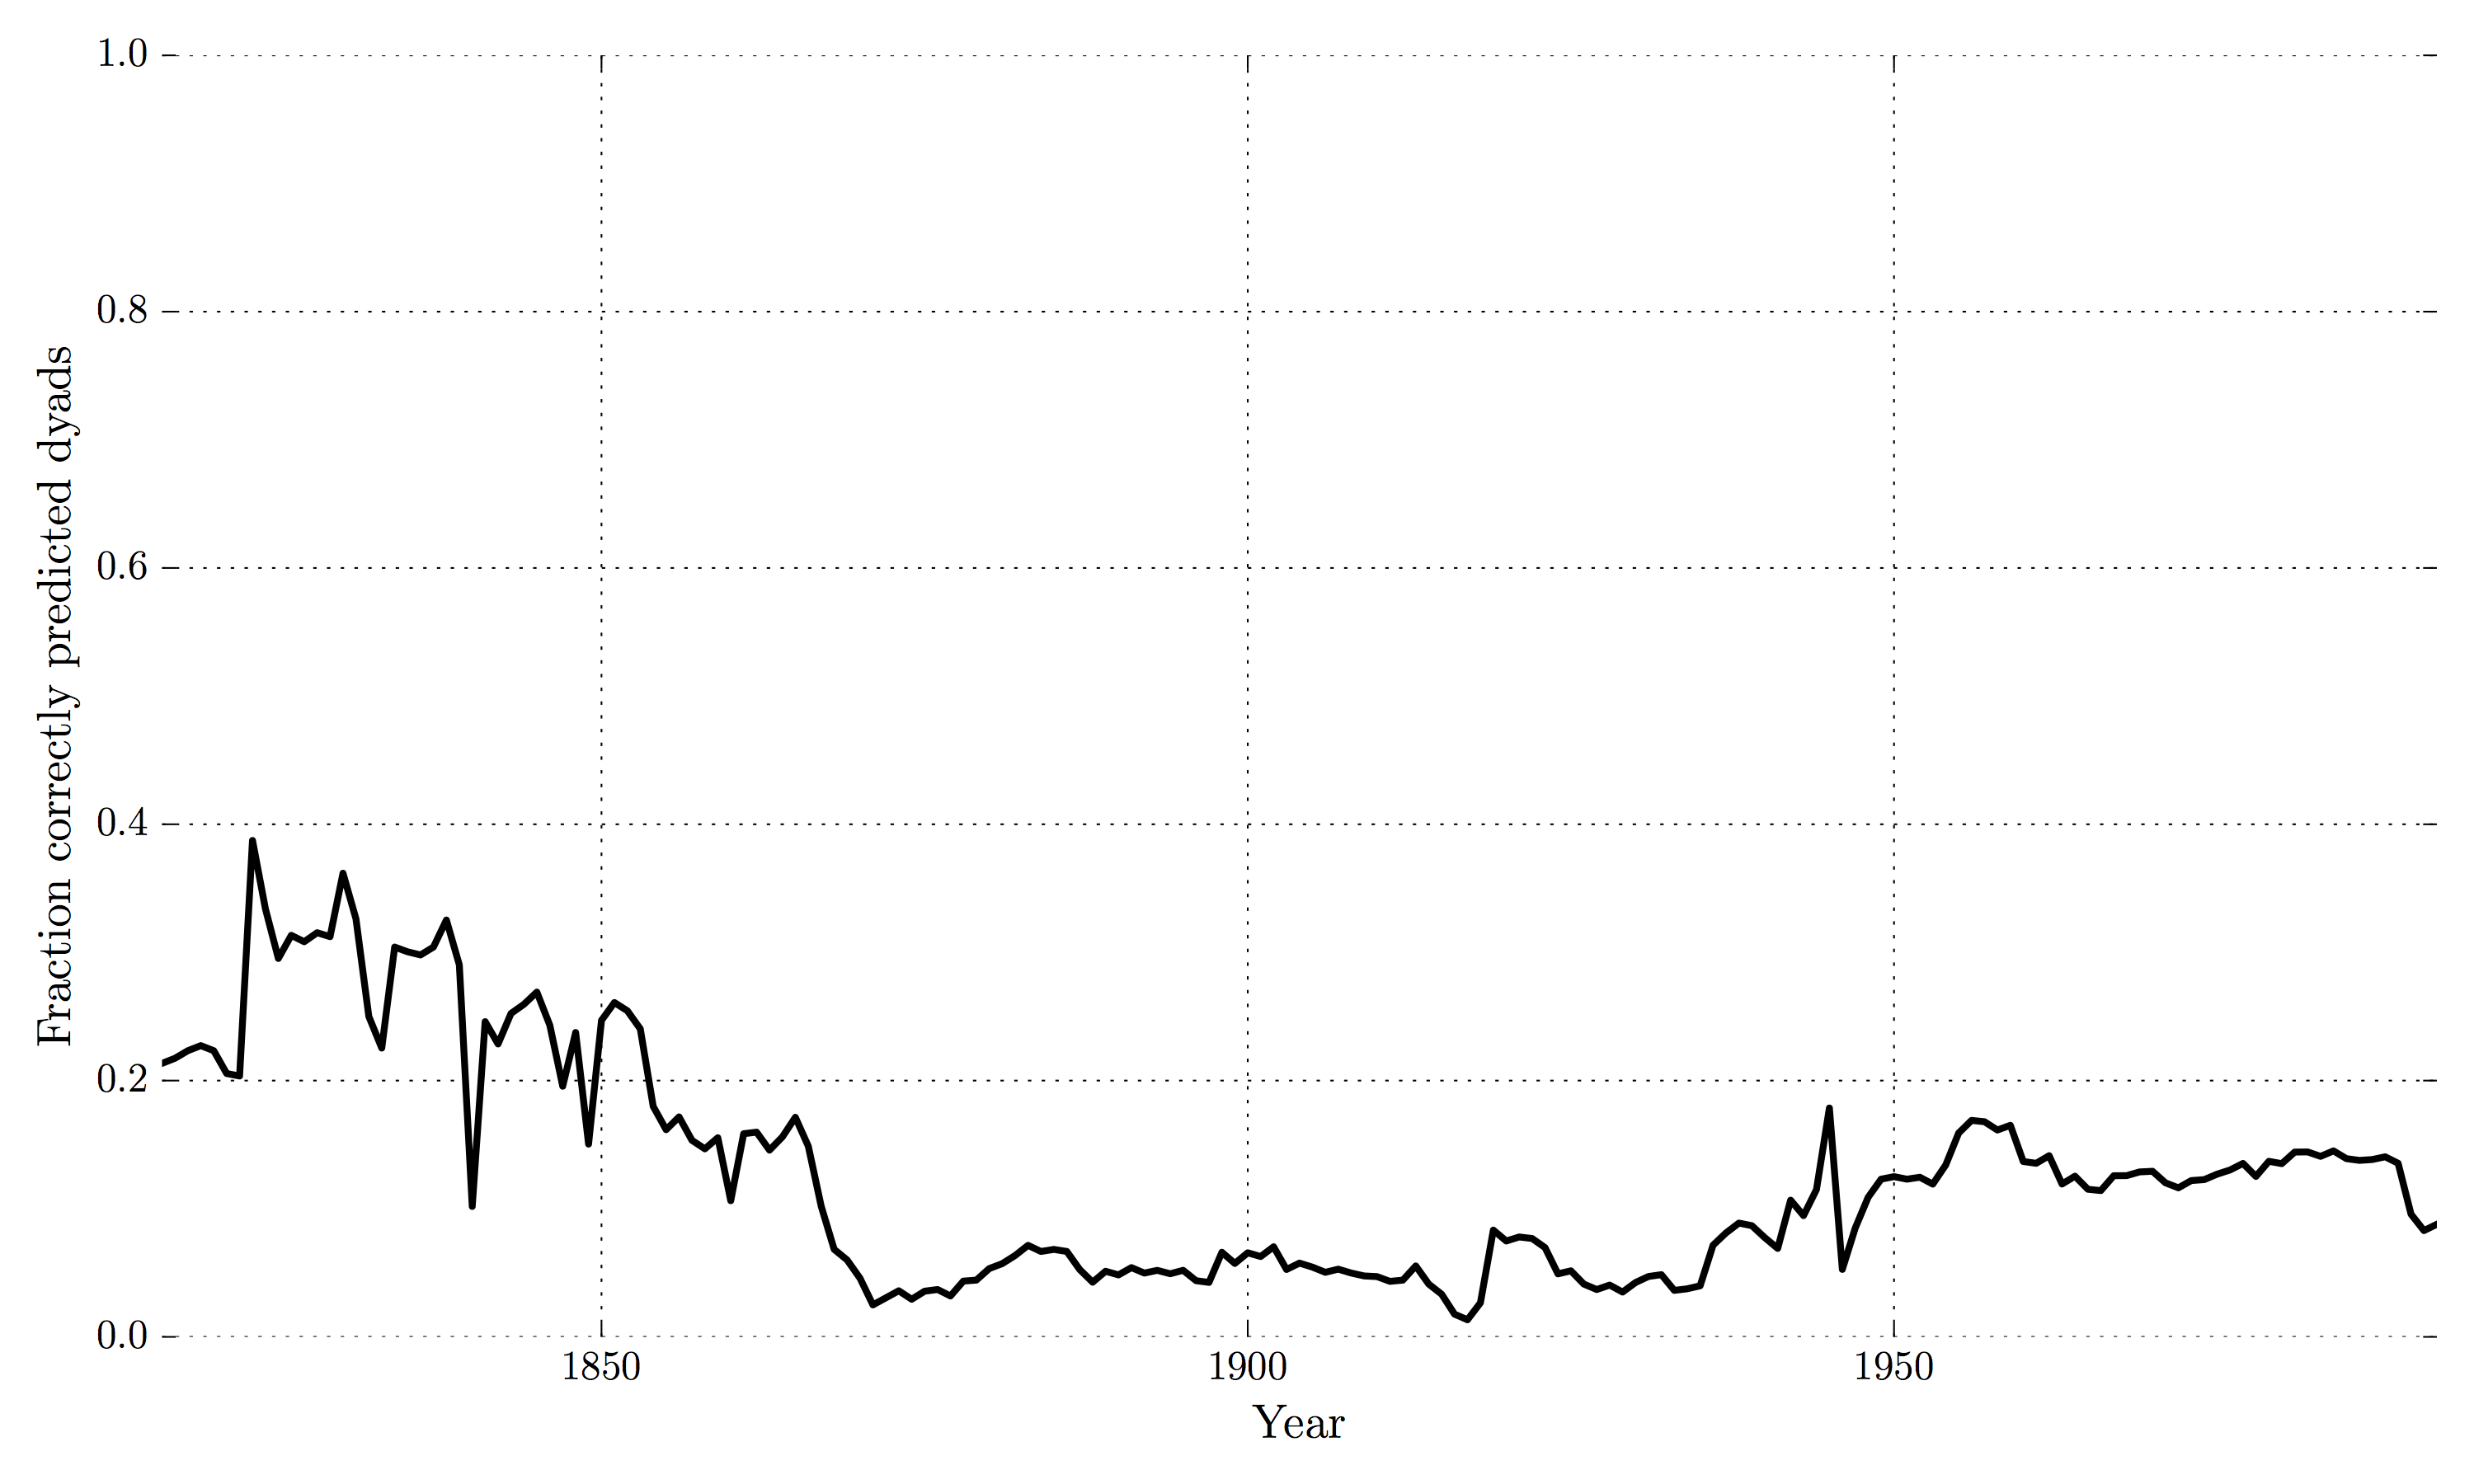
\includegraphics[width=0.7\textwidth]{WarReason/Figures/EQ_correct}
	        \caption{IIG Equilibrium Outcome}
	        \label{fig:eq_correct}
	    \end{subfigure}

	    \begin{subfigure}[t]{0.7\textwidth}
	        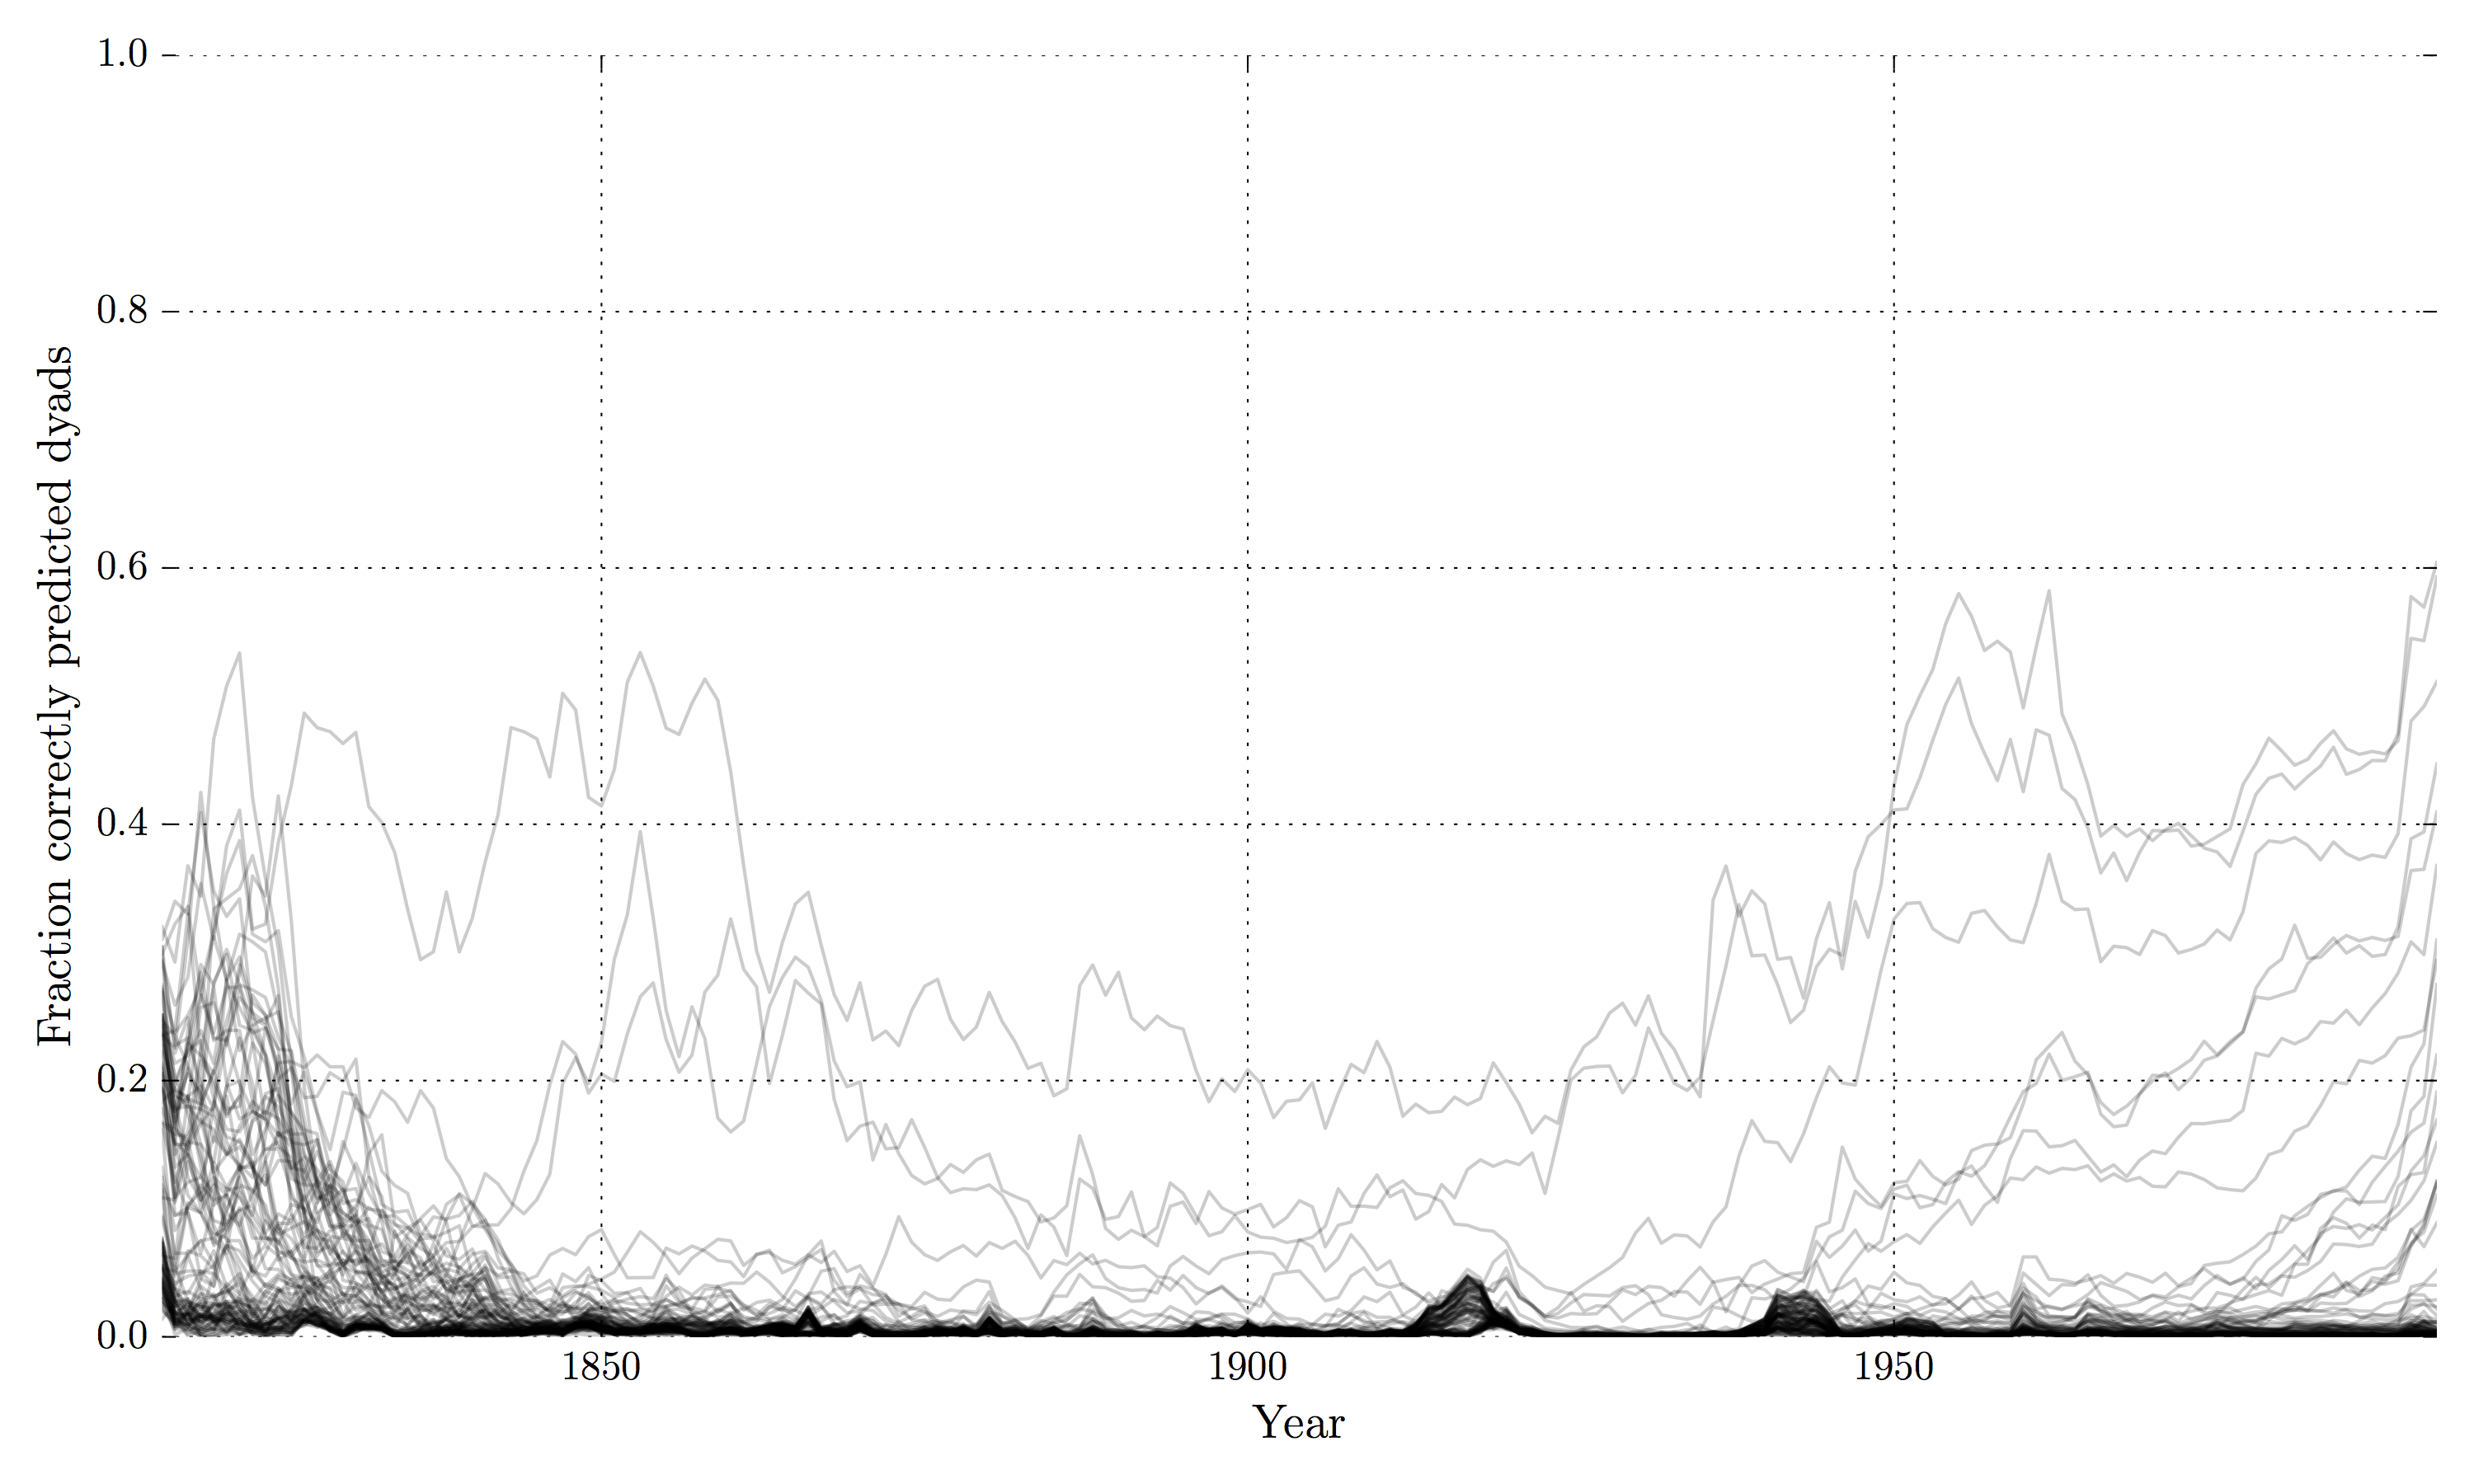
\includegraphics[width=\textwidth]{WarReason/Figures/RL_correct}
	        \caption{Reinforcement Learning Model}
	    \end{subfigure}
	    \begin{subfigure}[t]{0.7\textwidth}
	        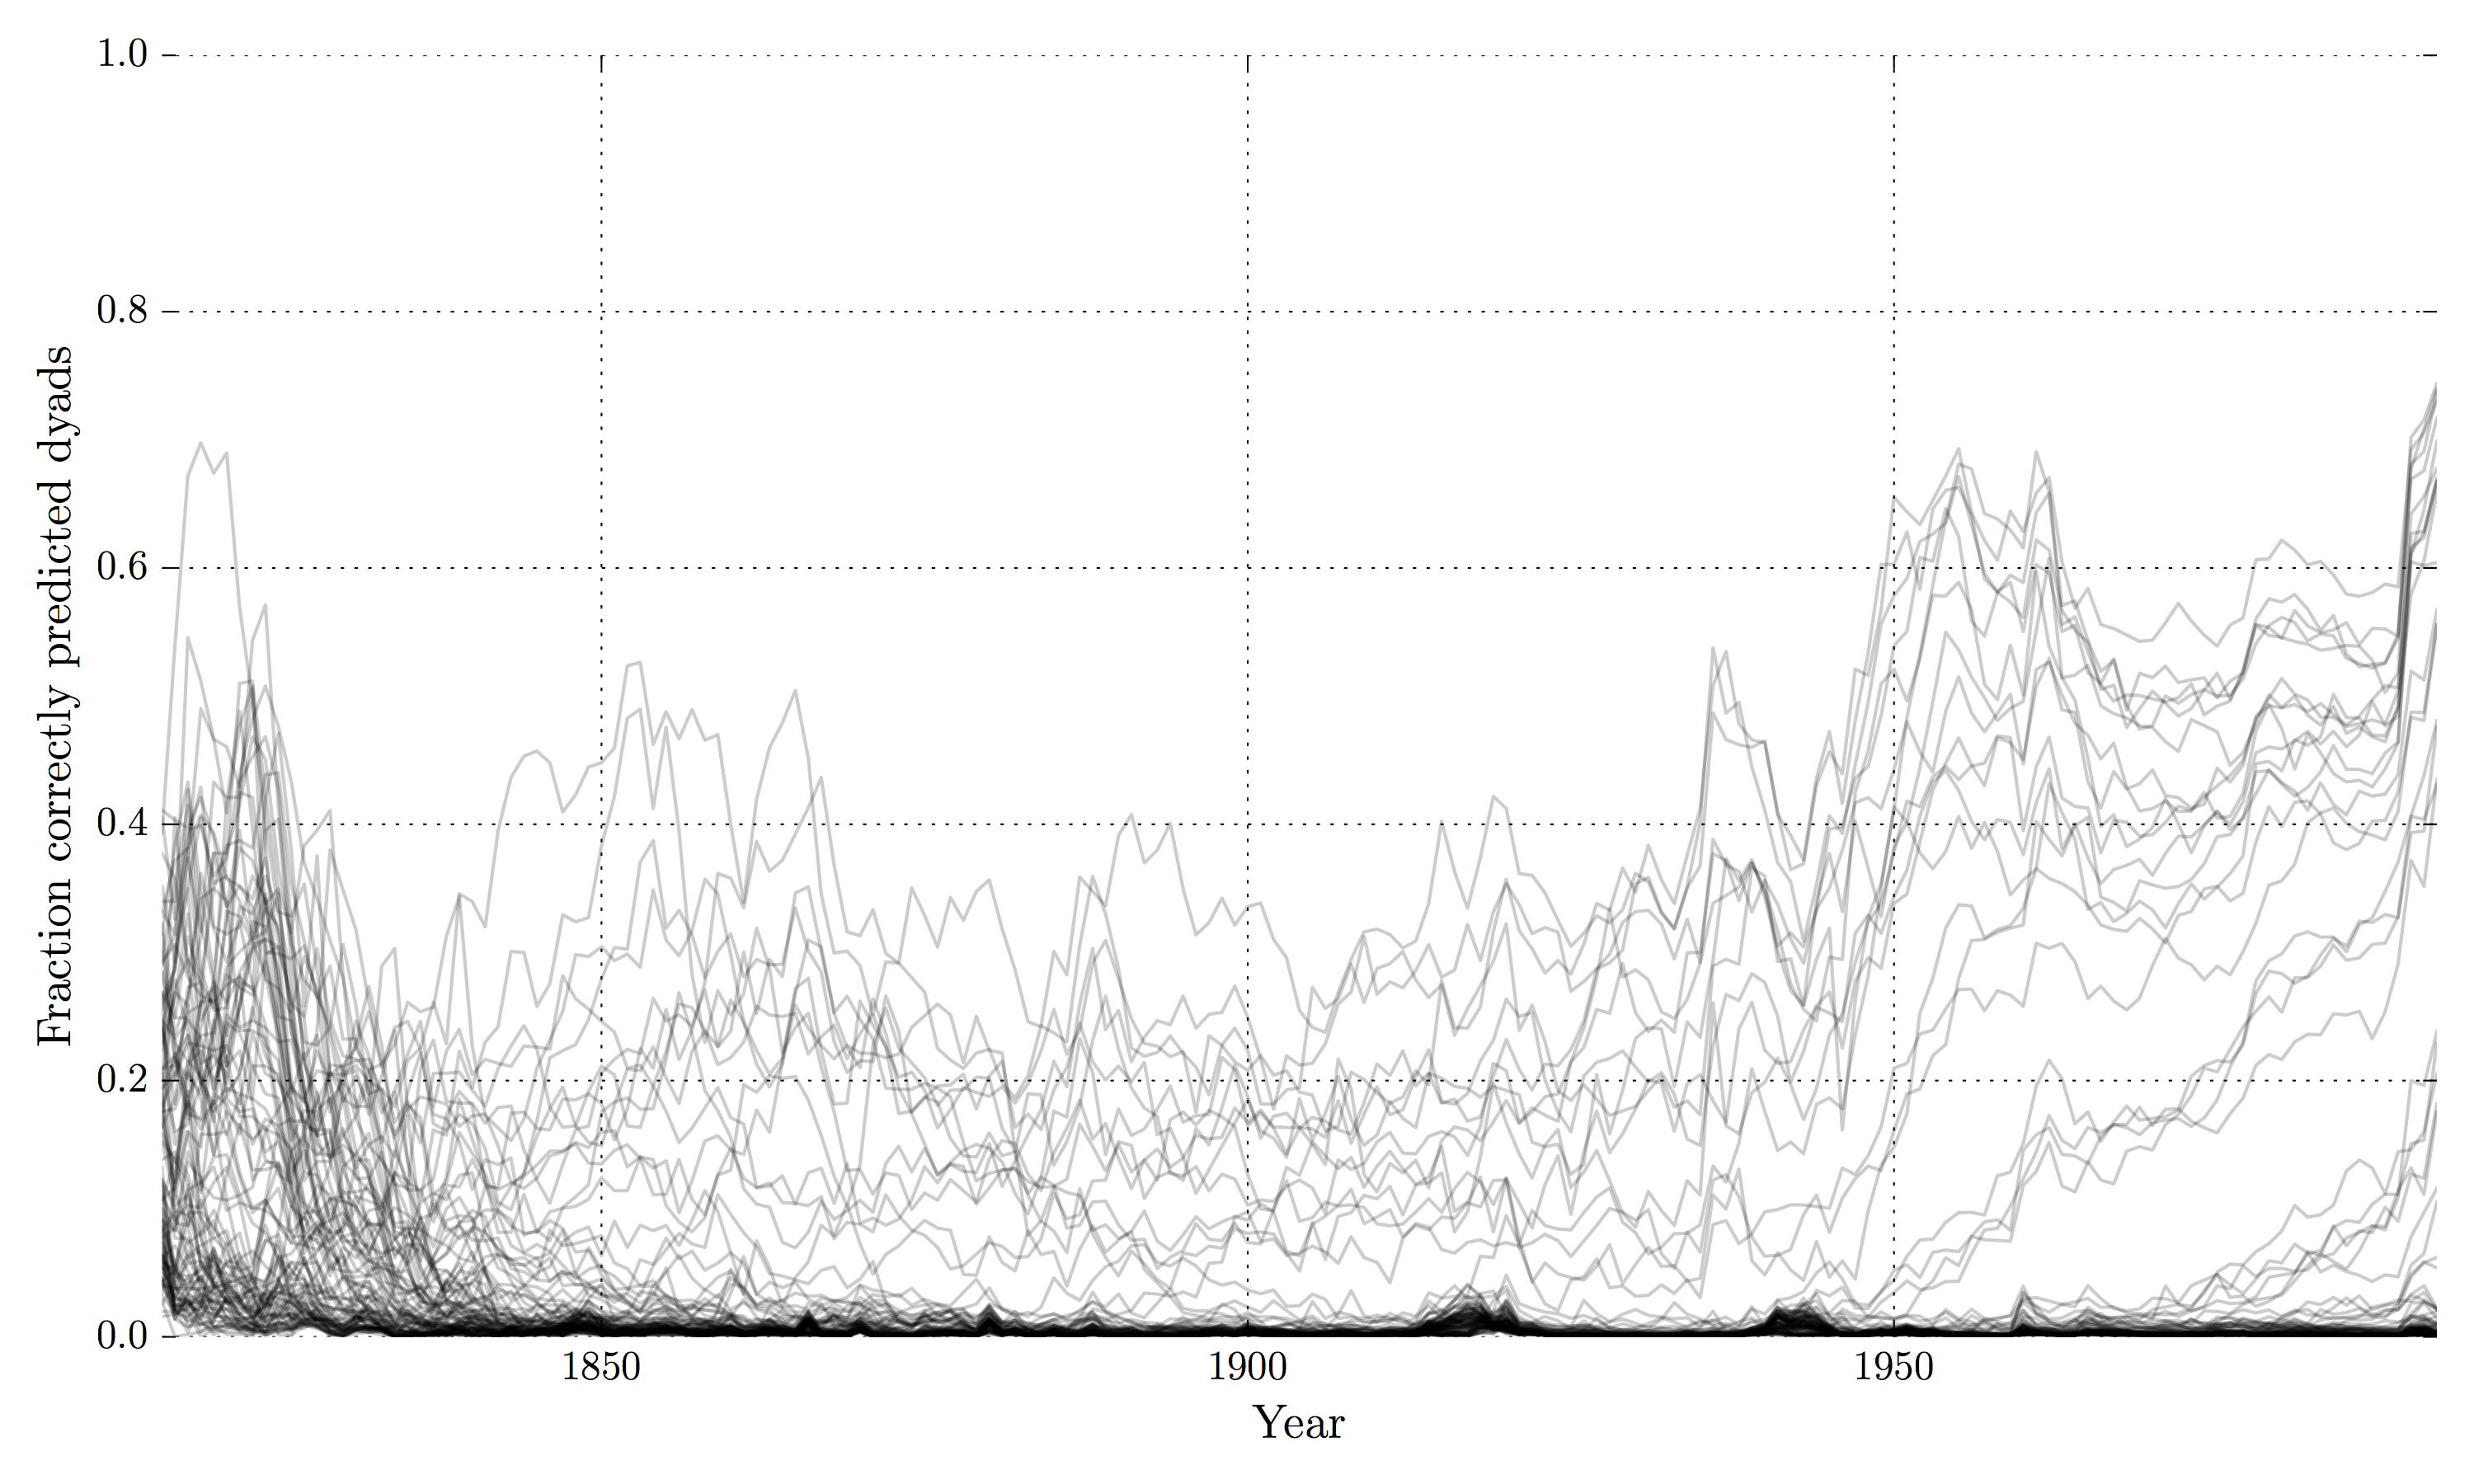
\includegraphics[width=\textwidth]{WarReason/Figures/CB_correct}
	        \caption{Case-Based Reasoning Model}
	    \end{subfigure}

	    \caption{Fraction of Interactions with Correctly-Predicted Outcome}
	    \label{fig:ex2_correct}
	    \figSpace
	\end{figure}

\end{landscape}

With these results in hand, we can proceed to test whether the model outcomes are a statistically useful predictor of the observed events. As demonstrated in Figure \ref{fig:eq_correct}, the IIG equilibrium is not a direct prediction of observed events; instead, \citet{bdm_1992} and \citet{bennett_2000} use it as a statistical predictor, arguing that estimating a particular equilibrium makes it more likely (though far from certain) that we will observe a corresponding event in the historic data. I apply a similar test to the model outputs. Since the learning models take some number of interactions for their initial learning, it is sensible to drop these early interactions from our analysis as a burn-in period. I could not identify a formal method to determine how long this period ought to be. Based on the traces in Figure \ref{fig:ex2_traces}, the main attractors across the decision models begin to appear at approximately 1850; for this reason, I choose this year as the cutoff for the burn-in period.

I start by replicating the findings of the prior studies. Table \ref{table:eq_regressions} shows the results of logistic regressions with the observed events of each post-1850 dyad as the dependent variables and the IIG equilibria as the independent variables \footnote{Strictly speaking, the correct regression for this case is a multinomial logit, as in \citet{bennett_2000}, since the outcomes of each interaction are mutually exclusive. However, the datasets produced by the 105 instantiations of each model are too large for a multinomial logit to be computationally tractable. In order to keep the model tractable, I treat each outcome as an independent variable. This method provides a worse fit, but allows the coefficients to be interpreted the same way.}. This is a simplified model, without many of the controls (e.g. for polity type, or length of peace) introduced by \citet{bennett_2000}. These regression results are comparable to those reported in \citet{bennett_2000}, providing moderate support for the hypothesis of the IIG equilibrium as an outcome predictor prior to adding in the various controls. More importantly, these results provide a baseline against which we may compare the results of similar regressions using the decisionmaking model interaction results.

%% table:eq_regressions showing logit results via IIG Equilibrium outcomes goes here

%% table:ex1_regressions and table:ex2_regressions GO ABOUT HERE, showing coefficients from RL and CB logits.

Tables \ref{table:rl_regressions} and \ref{table:cb_regressions} show the results of the same logistic regressions on the outcomes of the post-1850 interactions in the RL and CB models, respectively. The coefficients for both models as well as the equilibrium model are shown visually in Figure \ref{fig:coef_plots}, below. We can see that the learning model coefficients are similar to those of the equilibrium models, showing moderate support for the hypothesis that the model outcomes are a predictor of the observed outcome. The level of support varies between outcome types. For Acquiesce events, the coefficients on the corresponding model outcomes are significant and positive, while those on the opposite outcome (the acquiescence of the other party) are negative. However, this is not the case for Capitulate events, where capitulation outcomes in both directions have a positive coefficient. Importantly, War and Negotiation outcomes are both positive predictors of observing corresponding events. However, War outcomes are also predictors of observing Negotiation events -- which suggests that the model is correctly capturing cases where a conflict is likely, but that some of those conflicts are in fact resolved via negotiation rather than war. Similarly, note that the Capitulation outcomes are also positive predictors of War events, and vice versa. These outcomes are adjacent to one another on the game tree, which provides support for the structure of the game tree itself. It suggests that the model agents are playing down to the correct subgame of the game tree, with one agent making a single move different from what was observed.

\begin{figure}[h!]
	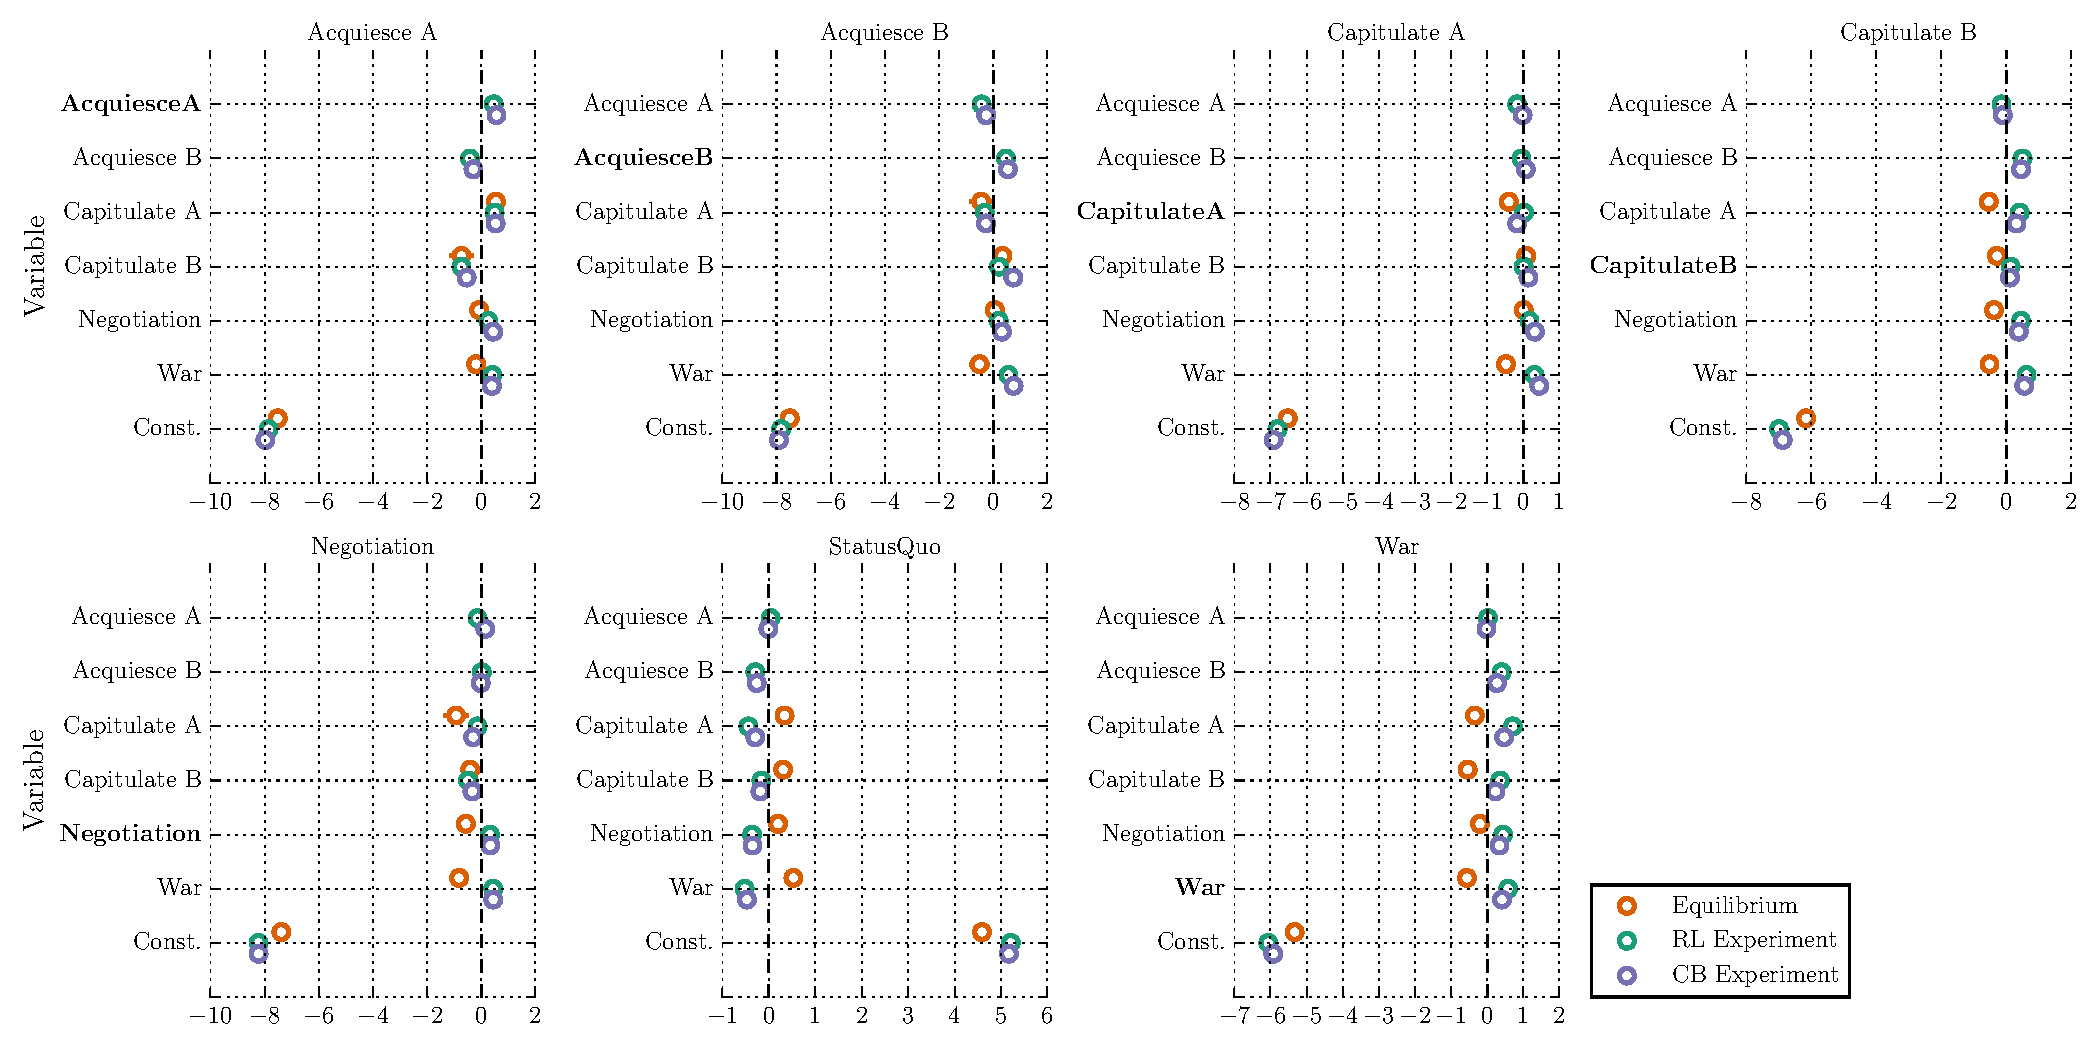
\includegraphics[width=\textwidth]{WarReason/Figures/WarReason_Coeffs.pdf}
    \caption{Logistic Regressions Coefficient Plots}
    \label{fig:coef_plots}
    \figSpace
\end{figure}

\begin{landscape}
\begin{table}
	\begin{center}
		\caption{IIG Model Equilibrium -- Logistic Regressions}
		\label{table:eq_regressions}
	\begin{tabular}{lccccccc}
	\hline
	             & Capitulate A & Capitulate B & Acquiesce A & Acquiesce B & Negotiation & War      & StatusQuo   \\
	\hline
	Acquiesce A & -0.40***      & -0.54***     & 0.54***     & -0.45**     & -0.92***    & -0.34*** & 0.34***   \\
	            & (0.13)        & (0.12)       & (0.17)      & (0.22)      & (0.24)      & (0.07)   & (0.05)    \\
	Acquiesce B & 0.08          & -0.29***     & -0.73***    & 0.34**      & -0.41**     & -0.54*** & 0.31***   \\
	            & (0.11)        & (0.10)       & (0.23)      & (0.17)      & (0.19)      & (0.07)   & (0.05)    \\
	Negotiation & 0.01          & -0.38***     & -0.08       & 0.06        & -0.56***    & -0.20*** & 0.20***   \\
	            & (0.08)        & (0.07)       & (0.14)      & (0.14)      & (0.14)      & (0.05)   & (0.03)    \\
	War A       & -0.48***      & -0.52***     & -0.19       & -0.52***    & -0.86***    & -0.57*** & 0.53***   \\
	            & (0.11)        & (0.09)       & (0.17)      & (0.18)      & (0.19)      & (0.06)   & (0.04)    \\
	War B       & 0.81          & 0.44         & -24.50      & 1.79*       & 2.36***     & 0.72     & -0.98***  \\
	            & (1.00)        & (1.00)       & (512568.77) & (1.01)      & (0.72)      & (0.58)   & (0.36)    \\
	Const.      & -6.52***      & -6.16***     & -7.51***    & -7.51***    & -7.38***    & -5.33*** & 4.59***   \\
	            & (0.08)        & (0.06)       & (0.13)      & (0.13)      & (0.12)      & (0.04)   & (0.03)    \\
	\hline
	\hline
	\multicolumn{8}{l}{Standard errors in parentheses.} \\
	\multicolumn{8}{l}{* $p<.1$, ** $p<.05$, *** $p<.01$} \\
	\end{tabular}
	\end{center}
	\tableSpace
\end{table}

\begin{table}
	\begin{center}
		\caption{Reinforcement Learning Model -- Logistic Regressions}
		\label{table:rl_regressions}
	\begin{tabular}{lccccccc}
	\hline
	             & Capitulate A & Capitulate B & Acquiesce A & Acquiesce B & Negotiation & War      & StatusQuo   \\
	\hline
	Acquiesce A  & -0.17***     & -0.15***     & 0.46***     & -0.43***    & -0.14**     & 0.02     & 0.04***     \\
	             & (0.03)       & (0.03)       & (0.04)      & (0.05)      & (0.06)      & (0.02)   & (0.01)      \\
	Acquiesce B  & -0.05**      & 0.50***      & -0.42***    & 0.47***     & 0.02        & 0.40***  & -0.29***    \\
	             & (0.02)       & (0.02)       & (0.04)      & (0.04)      & (0.05)      & (0.01)   & (0.01)      \\
	Capitulate A & 0.02         & 0.41***      & 0.49***     & -0.31***    & -0.14       & 0.71***  & -0.44***    \\
	             & (0.05)       & (0.05)       & (0.07)      & (0.10)      & (0.12)      & (0.03)   & (0.02)      \\
	Capitulate B & 0.01         & 0.13**       & -0.73***    & 0.21***     & -0.49***    & 0.36***  & -0.16***    \\
	             & (0.05)       & (0.06)       & (0.13)      & (0.08)      & (0.14)      & (0.03)   & (0.02)      \\
	Negotiation  & 0.17***      & 0.45***      & 0.26***     & 0.20***     & 0.32***     & 0.44***  & -0.36***    \\
	             & (0.02)       & (0.02)       & (0.03)      & (0.03)      & (0.04)      & (0.01)   & (0.01)      \\
	War          & 0.31***      & 0.62***      & 0.41***     & 0.56***     & 0.44***     & 0.58***  & -0.52***    \\
	             & (0.02)       & (0.02)       & (0.03)      & (0.03)      & (0.04)      & (0.01)   & (0.01)      \\
	Const.       & -6.80***     & -6.99***     & -7.85***    & -7.83***    & -8.22***    & -6.06*** & 5.21***     \\
	             & (0.02)       & (0.02)       & (0.03)      & (0.03)      & (0.04)      & (0.01)   & (0.01)      \\
	\hline
	\hline
	\multicolumn{8}{l}{Standard errors in parentheses.} \\
	\multicolumn{8}{l}{* $p<.1$, ** $p<.05$, *** $p<.01$} \\
	\end{tabular}
	\end{center}
	\tableSpace
\end{table}

\begin{table}
	\begin{center}
	\caption{Case-Based Reasoning Model - Logistic Regressions}
	\label{table:cb_regressions}
	\begin{tabular}{lccccccc}
	\hline
	             & Capitulate A & Capitulate B & Acquiesce A & Acquiesce B & Negotiation & War      & StatusQuo   \\
	\hline
	Acquiesce A  & -0.02        & -0.11***     & 0.56***     & -0.26***    & 0.15***     & -0.02    & -0.01      \\
	             & (0.02)       & (0.02)       & (0.03)      & (0.04)      & (0.04)      & (0.01)   & (0.01)     \\
	Acquiesce B  & 0.07***      & 0.45***      & -0.29***    & 0.54***     & -0.02       & 0.27***  & -0.26***   \\
	             & (0.02)       & (0.02)       & (0.04)      & (0.03)      & (0.04)      & (0.01)   & (0.01)     \\
	Capitulate A & -0.17**      & 0.31***      & 0.53***     & -0.27**     & -0.30**     & 0.47***  & -0.29***   \\
	             & (0.07)       & (0.06)       & (0.09)      & (0.13)      & (0.15)      & (0.03)   & (0.02)     \\
	Capitulate B & 0.14**       & 0.11*        & -0.54***    & 0.74***     & -0.33**     & 0.23***  & -0.18***   \\
	             & (0.06)       & (0.06)       & (0.15)      & (0.08)      & (0.15)      & (0.04)   & (0.03)     \\
	Negotiation  & 0.32***      & 0.38***      & 0.44***     & 0.32***     & 0.33***     & 0.34***  & -0.35***   \\
	             & (0.01)       & (0.01)       & (0.02)      & (0.02)      & (0.02)      & (0.01)   & (0.01)     \\
	War          & 0.44***      & 0.55***      & 0.39***     & 0.75***     & 0.44***     & 0.41***  & -0.47***   \\
	             & (0.01)       & (0.01)       & (0.02)      & (0.02)      & (0.03)      & (0.01)   & (0.01)     \\
	Const.       & -6.91***     & -6.88***     & -7.97***    & -7.91***    & -8.22***    & -5.92*** & 5.17***    \\
	             & (0.01)       & (0.01)       & (0.02)      & (0.02)      & (0.02)      & (0.01)   & (0.00)     \\
	\hline
	\hline
	\multicolumn{8}{l}{Standard errors in parentheses.} \\
	\multicolumn{8}{l}{* $p<.1$, ** $p<.05$, *** $p<.01$} \\
	\end{tabular}
	\end{center}
	\tableSpace
\end{table}

\end{landscape}

\section{Discussion}\label{discussion}

In this chapter, I have presented an attempt to use agent-based modeling as a bridge between several schools of thought and lines of research in the study of states' decisionmaking in the face of international conflicts. The ABM perspective allows us to build on a previous, well-studied model of international relations, and to view the rational-choice, equilibrium-playing behavior as only one of many possible models of decisionmaking which may be implemented and tested within a computational framework. I have presented two such decisionmaking models, which are both simplified but psychologically and organizationally plausible. I then used these models to drive the decisionmaking of agents within two simulated international systems: a simplified notional one, and one based on historic data and a well-validated interaction model.

The notional system allows us to focus on the properties of the decisionmaking models themselves by controlling the complexity of the system. Across both the static and dynamic world variants, we see that both the reinforcement learning (RL) and case-based learning (CB) decisionmaking models converge to sets of behaviors that play the rational equilibrium strategies far more than randomly, though far less than perfectly. Close examination of interactions and model runs, as well as preliminary work not presented here, indicates that the agents play close to equilibrium when the equilibrium utilities are substantially greater than those from the non-equilibrium outcomes; when these utilities are closer, convergence is reduced. This suggests an important observation: these decisionmaking rules are producing satisficing outcomes. They collectively find distributions of strategies that yield positive utilities, and thus have little incentive to explore and arrive at the equilibrium strategy with only slightly higher payoffs. 

Examination of the model traces shown in Figures \ref{fig:sc1_traces} and \ref{fig:sc2_traces} suggests that the convergence to near-equilibrium play happens either very quickly or not at all. This provides validity to the model's `cold start' assumption of having all agents start each run with no information or initial weights, and for discarding only a relatively small fraction of early interactions as a burn-in period. This, in turn, helps address the objection that the real decisionmakers in the early periods covered by the model already had previous experience to draw on, unlike the model agents. Furthermore, comparison of the equilibrium play by learning rate shown in Figures \ref{fig:sc1_boxwhiskers} and \ref{fig:sc2_boxwhiskers} suggests there is not a qualitative difference between the performance of the agents at the different rates. This reduces the need to repeat the IIG experiments with different learning rates, which is limited by the time and computational resources required for each run.

Finally, and somewhat surprisingly, the the CB model does not consistently outperform the context-free RL model. In the static world variant, the CB model does generally perform better than the RL model, as it allows agents to learn a particular set of weights to use against each other agent. However, in the dynamic world variant, the changing agent properties generate larger case libraries for each agent, which in turn leads to a higher probability of querying a case with a different equilibrium than the current one. While this may appear at first to be an artifact of the model specifications, it may in fact also be capturing a feature present in real-world reasoning: that the most-similar historic analogy to a particular case may not in fact be the correct analogy, in that the lessons learned from one will not lead to the desired or expected outcome in the other.

The International Interaction Game variant offered a greater number of agents, with greater interaction complexity and less structured changes in agent properties and potential payoffs. Despite this, both decisionmaking models again rapidly yield a higher than random share of interactions with an equilibrium outcome. Beginning with no initial weights or other information, the agents appear to rapidly learn weights (essentially mixed strategies) which approach the equilibrium. Whereas the Small Crisis model saw an approximately normal distribution of traces and performance across the quality space, the IIG seems to exhibit several attractor regions which recur across runs and between decisionmaking models. This suggests that the structure of the international system (at least as captured by the data and IIG calculations) drives the agents to learn particular distributions of strategies -- and that these strategy sets are satisficing. In particular, the fact that there are two attractors at different quality levels suggests that there are two sets of satisficing strategies that the agents converge to, with one much closer to the equilibria than the other.

Both the RL and CB models are underpredictive of overall observed events -- as, indeed, is the baseline rational model. A large part of the reason for this is that the vast majority of interactions are politically irrelevant dyads between distant countries; even if the IIG utility calculations indicate that one actor has utility to gain from threatening force against the other, this utility gain is largely abstract, with no actual concrete disputes which may lead to war. For this reason, the majority of RL an CB runs, like the rational IIG model, over-predict non status quo outcomes. However, an advantage that the agent-based model has over the game-theoretic original is that its stochasticity produces a range of traces -- and, as shown in Figure \ref{fig:ex2_correct}, some of those are discovered to be far more predictive. This suggests that the set of strategies that are more likely to produce interaction outcomes actually matching observed events are satisficing as well, despite being far from the equilibrium strategy set. The CB decision model appears to have an advantage over the RL model in terms of both its overall rate of correctly generating observed events, and in terms of the number of iterations consistently generating correct outcomes.

Applying the logistic regression methodology used by \citet{bennett_2000} to test the explanatory and predictive power of the different models indicates that the RL and CB models are in line with the original rational model, and do not have radically stronger or weaker predictive power in the aggregate. There are no event categories for which the sign or significance on the corresponding coefficients are different, or where there is a substantial difference in the magnitude of those coefficients. There is no event which is obviously better predicted by the equilibrium than the model results, and the Negotiation equilibrium has a negative coefficient on the corresponding event, in contrast to the positive coefficients both learning models produce.

With these results in hand, we may directly address the underlying question of crisis decisionmaking when addressing potential international conflicts. Multiple agents using both the context-free reinforcement learning decisionmaking model and the case-based learning model do not converge to perfectly rational equilibrium behavior across multiple models of the international system. Nevertheless, the behaviors and outcomes emerging from the agents' interactions often approach the equilibria. If the real-world actors are making decisions in ways that resemble the RL and CB models, these results suggest they will converge to rational-like behavior. This supports the assertion that the assumption of rationality is useful as a simplified model, even if it is not descriptive of the procedure by which decisions are made -- a specific case of the broader argument put forward by \citet{friedman_1953}. However, the rational model does not appear to be a better predictor of observed events than the learning models. Thus, there does not appear to be strong support for a hypothesis that the rational equilibrium provides a better predictor than the alternative model outcomes; or more generally, for the hypothesis that agents exhibiting perfect rationality provide a better model for states than agents utilizing even simple forms of learning. This means we do not need to rely on the assumption of rationality -- we may implement more plausible models of decisionmaking and achieve similar predictive results
% RAX: cite Friedman 1953 / "principle of unreality"? DONE

Furthermore, the learning models have an advantage over the purely rational model in that they can converge to sequences of outcomes that are non-equilibrium but nevertheless satisficing, under the given utility assumptions. Importantly, we see that the models may converge to outcome sequences which are a better match for historic observations. This provides evidence that, under the IIG's utility calculations, the observed interactions between states may themselves be satisficing, despite often being non-equilibrium outcomes. Finally, this in turn suggests that the learning models provide a plausible explanation for the difference between the equilibria and observed outcomes. If the IIG provides a valid estimate for actors' preferences between outcomes and approximation of the process by which crises escalate, models of decisionmaking driven by past experiences are capable of producing (and hence, explaining) observed history in a way that a strategic rationality model is not.

The work presented in this chapter suggests several opportunities for extension and expansion. There are additional decisionmaking models which could be implemented with relative ease, and tested using the same methods. I conducted initial tests of a learning model in which all agents shared a single case library, allowing them to learn from each other's experience; while this variant appeared to produce greater convergence to equilibrium, its computational costs prevented the full experiments needed to include it here. Other decision models may move away from the learning paradigm entirely in favor of simple rules (e.g. tit-for-tat), expert-derived heuristics, or other methods. I also conducted initial tests with relaxing the `cold start' assumption. Alternatives include training agents with the correct outcomes (either equilibrium or historic) over an early subset of cases, as well as having only a subset of agents utilizing a learning model while the others are rational. Both training to equilibrium and adding rational-playing agents appeared to generate a higher rate of equilibrium play -- though, as we have covered, this is unlikely to improve the models' fit to data.

Future work may also have the model code itself performing the computations for the utility estimations which are currently provided by EUGene. Methods for this are present in the code already, but were not used here -- both due to the computational costs of these operations (particularly risk tolerance estimation, as detailed in Footnote \ref{fn:eugene_risk}) and in order to maintain consistency with previous work. The model's object-oriented architecture allows for alteration, and experimentation with, all the elements of the various sub-models, providing a wide range of additional hypotheses to be tested. These may involve something as simple as replacing tau similarity with a different measure, changing the payoff estimations, utilizing a different game tree, or even endogenizing the change in agent properties based on the outcome of each interaction. This means that the code presented here is not simply a tool for testing a few simple models of state decisionmaking, but the basis for a framework for much broader data-anchored agent-based models of international crises, and international relations more broadly.


\chapter[BDM's EUM as ABM]{BDM's EUM as ABM: Agentizing the Expected Utility Model}

\section{Introduction}

In a series of papers and books across several decades, Bruce Bueno de Mesquita (commonly referred to as BDM) has presented and applied several versions of a forecasting model to predicting everything from internal Iranian power struggles \citeyearpar{bdm_1984} and European regulation negotiations \citeyearpar{bdm_1994} to the course of the entire Cold War \citeyearpar{bdm_1998}. The model is intended to simulate the iterative negotiation process between multiple actors, identifying where they compromise and where they attempt to coerce one another. It has attracted widespread attention (particularly by the standards of political science models): it was the subject of a special journal issue \citep{kugler_1997}, and was featured in a popular-audience TED talk \citep{bdm_2009} and book \citep{bdm_2010}. It has also, reportedly, been successfully applied by the Central Intelligence Agency \citep{feder_1992}, as well as numerous commercial clients of Decision Insights, Incorporated (a consulting firm BDM co-founded), for prediction as well as decision support \citep{root_2013}. The model was even the subject of a lawsuit by that company against a rival \citep{dii_2011} accused of stealing the model. 

Such a universal political forecasting model is worth examining in detail. BDM and his collaborators have described the model extensively \citep{bdm_1984,bdm_1994,bdm_1997,bdm_2002,bdm_2011}, but have never published the full specifications, and in particular never made the underlying code available. Several attempts have been made to replicate it from published material \citep{scholz_2011,kimbrough_2014,mckibben_sanders_2014}, but none of these have successfully fully reproduced its reported results. Indeed, as \citet{scholz_2011} document, some details of the model appear to have changed over time\footnote{These changes suggest that there is not a single `original' model to reproduce. Nevertheless, as BDM does not clearly demarcate different generations or variants, I will use phrase `original model' in this chapter to refer to my overall understanding of the model. My own implementation primarily followed the description provided in \citet{bdm_2002}.}, and testimony in the \citet{dii_2011} lawsuit states that the commercial version of the model contains trade secrets not reproducible from the public literature. There have also been several attempts to develop similar models: these include an internal CIA variant \citep{feder_1992}; the Senturion toolkit \citep{abdollahian_2006} (the competitors' model which triggered the lawsuit mentioned above); at least one more proprietary model that I am aware of; and the \citet{wise_2015a} Toolkit for Behavioral Analysis. Of these, only the last is open source; the rest are proprietary commercial products.

BDM has characterized the model as grounded in micro-economics \citep{bdm_1994} and game theory \citep{bdm_2002,bdm_2009,bdm_2010}, and often refers to it as the Expected Utility Model (EUM) \citep{bdm_1984} -- borrowing a key term from game theory and economics. Indeed, the EUM bears many of the hallmarks of a formal model. \citet{scholz_2011} describes the model's underlying interactions as an extensive-form game tree. Several of the model's internal specifications closely resemble those used in the International Interaction Game (IIG) \citep{bdm_1992}, the game-theoretic model of international conflict described in the previous chapter, and \citet{bdm_2011} proposes an update to the model which directly incorporating the IIG's extensive-form tree as well. Yet despite the game-theoretic components, the model bears some clear differences from conventional game theory. It is intended to model and predict particular real-world interactions rather than to identify general patterns and theories \citep{snidal_1985}. None of the papers discussing the model have analyzed it in closed form to identify and parameterize its equilibria, and it is unclear whether such equilibria exist, or are meaningful. Indeed, the problem of identifying formal equilibria of games with more than two players becomes rapidly intractable \citep{papadimitriou_2005}. Thus, unlike in the majority of game theory models, the players are not assumed to be perfectly rational; indeed, they are explicitly boundedly-rational, using a variety of heuristics and looking at most one step ahead \citep{bdm_2002}. Finally, the model is implemented computationally, with the overall model, and each actor within it, executing set calculations and methods sequentially, and updating accordingly. While the model is largely described in terms of the specific calculations the agents make, I argue that these calculations are best viewed as particular sub-models rather than the model itself. In fact, another model, the \citet{stokman_1994} logrolling model, which takes the same inputs as the EUM and is intended for comparison with it, is explicitly described as an object-oriented computational model. Similarly, \citet{root_2013} also describe the model as agent-based. Understanding the model as an ABM emphasizes that the numeric calculations are not necessarily the most important components of it; the particular agent behavior rules, and the way the model sequences them, are equally important. Furthermore, treating the model as an ABM suggests additional methodological tools we can use to analyze it, such as sensitivity analyses and parameter sweeps \citep{gilbert_2005}.

Unlike the International Interaction Game presented in the previous chapter, the EUM cannot be viewed as a direct translation of a particular qualitative theory into model form. To be sure, several components of the model are grounded in specific previous work. The definition, and significance, of the median voter position are drawn from the \citet{black_1948} economic analysis of collective decisionmaking; the risk propensity calculation, meanwhile, is drawn from Prospect Theory \citep{kahneman_1984} as detailed further in Section \ref{risk_update}. Beyond that, however, the model draws general assumptions from Realist theories -- the political actors are unitary entities, rationally maximizing their utility and cooperating only inasmuch as such cooperation is in their immediate interest -- but its details (such as the expected utility calculations and the offer-based interactions) cannot be traced to particular qualitative descriptions of state interactions, or political interactions more broadly. Put another way: the model is itself a theory of political interaction, competition and decisionmaking.

This chapter attempts to address several inter-connected questions and issues. The EUM has been utilized in multiple papers and developed a receptive audience, making it interesting to study and replicate, in order to test its accuracy independently, understand its driving assumptions, and potentially enable us to use it in future research. In the course of this replication, I argue that the model is best understood as an agent-based model, making it an important example of an ABM with predictive power and both academic and policy relevance. Such models are rare in general, and all the more so in the realm of international relations. Finally, I argue that the model can serve as the basis for comparative modeling of political conflicts. By using fixed inputs and modifying the assumptions and theories embedded in the model code, we can directly compare the effects implied by these theories, and test their explanatory and predictive power. If a model variant utilizing one theory produces more accurate outputs than one using a different theory, this is evidence that the first theory is more correct with regard to the system being modeled. Such comparison is particularly important given the model's numerous sub-models and weak grounding in prior theories, as it allows us to test whether the assumptions the sub-models make contribute to or detract from the model's overall explanatory and predictive power.

I have attempted to reimplement the Expected Utility model as an object-oriented, agent-based computer simulation. In this chapter, I restate the model following the ODD (Overview, Design concepts, Details) outline \citep{grimm_2006}, highlighting the entities, variables and sub-models from which the model is assembled (Section \ref{model_description}). I describe my attempt to validate the model against previous results (Section \ref{verification}) and conduct a deep dive into a single model step to describe and verify its behavior (Section \ref{deep-dive}). I then discuss the assumptions embedded in the model structure and implementation (Section \ref{bdm_discussion}), and propose several sub-model variations which can be easily swapped into the model implementation. In Section \ref{sensitivity-analysis}, I describe a sensitivity analysis I conduct using artificial input data sets. In Section \ref{info_extraction} I describe the output data the model generates, which can be compared to empirical data or used for prediction. Finally, In Section \ref{icews}, I apply the model in a novel way, implementing several of my proposed model variants and comparing their outputs to micro-level political event data.

\section{Model Description} \label{model_description}

The following section is written approximately following the ODD protocol \citep{grimm_2006}. I first provide an overview of the model (Section \ref{overview}), including its purpose, and its agents and variables; I describe the sub-models, introduce a notation system to concisely reference different sub-model variants, and describe the computational structure used to implement it. I then describe the model in more detail (Section \ref{details}): how it is instantiated, and the specifics of the several sub-models which make it up. Unlike in an orthodox ODD description, I leave the model design concepts for Section \ref{bdm_discussion}, as they will be the points of study for the different model variants.

\subsection{Overview} \label{overview}

%% Purpose

The primary objective of the model is to predict the outcome of some `issue' which multiple different actors conflict on, or are negotiating over. It does this by simulating the iterative process by which these actors attempt to threaten or coerce one another into adopting their own preferred position, update their declared position in response to these threats, and come into conflict with one another. The issue under consideration may be as broad as the outcome of the Cold War, as in \citet{bdm_1998}, or as narrow as the chosen size of the Italian deficit \citep{feder_1992}. Nevertheless, each instantiation of the model is intended to focus on one particular issue, however defined.

%% State variables and scales

Each model instantiation consists of several actors, endowed with capabilities they can use to coerce each other or defend themselves from coercion, holding a position on the issue space, and possessing a salience value representing the importance they attach to the issue. The issue space is represented as a continuous one-dimensional line segment; between the maximum and minimum positions, any position represents a possible outcome, which agents can seek. For the sake of convenience, I normalize the issue space for all instantiations to the ${[0, 1]}$ range. 

Each agent is defined by several values, as summarized in Table \ref{table:model_vars}. I particular, they have three key values: position, salience and capability.
\begin{description}
    \item[Position] refers to the issue outcome or stance this actor publically supports at the moment, as projected onto the one-dimensional issue space. Agents may change their position as part of each step.

    \item[Salience] represents the importance the actor attaches to this particular issue, compared to the other actors. In practice, this refers to the fraction of coercive resources (capability) the actor is willing to devote to this particular issue. Salience is in the ${(0, 1]}$ range. It will also inform the other agent's belief of how likely the actor is to yield to threats. Unlike position, salience is not updated endogenously, though in some model variants it may change stochastically to simulate exogenous shocks.

    \item[Capability] represents the actor's coercive capacity, as relevant to the issue at hand. In some cases, it may be military force; however, in cases such as commercial negotiations, financial or regulatory influence may be more important; and in some cases, social capital or persuasive power may be the most relevant source of influence. Capability is continuous, and linearly additive, and the ratio of capabilities on either side of a bilateral conflict determines the probability of either side winning or losing. Since capability values only comes into play as ratios, they can be represented on any positive scale.
\end{description}

In addition, agents have several variables governing their decisionmaking and utility calculations. Key among these is risk propensity, which is used in utility calculations; risk propensity is a derivative property, determined each step by the position of the agent relative to all other agents. Two additional variables model the agents' beliefs about the future if they do not act. $Q_i$ is agent $i$'s believed probability that if they do not threaten an agent, that agent will nevertheless change its position. $T_i$ is the agent's belief in the probability that, if that other agents does change position, it will be towards the current median position. These last two variables are generally constant and identical for all agents in a model instantiation. Values of $0.5$ indicates maximum uncertainty, while $1$ and $0$ indicate certainty that agents will or will not move, and that that movement will be towards the median.

\begin{table}
\centering
\caption{Agent Variables}
\label{table:model_vars}
\begin{tabular}{cl}
    \hline
    Variable &  Description \\
    \hline
    $x_i$       &        Current position of agent $i$  \\
    $s_i$       &        Salience of agent $i$          \\
    $c_i$       &        Capability of agent $i$        \\
    \hline
    $r_i$       &        risk propensity of agent $i$  \\
    $Q_i$       &   Agent $i$'s belief that any other agent will move absent an offer from $i$. \\
    $T_i$       & Belief that other agent's movement will be towards median. \\
    \hline
\end{tabular}
\tableSpace
\end{table}

%% Process overview and scheduling

The model treats all conflicts as bilateral; however, other agents not directly involved in a particular bilateral conflict may contribute some of their own capability to one side or another, as specified in Equation \ref{eq:votes}. Each side of the conflict then has some total capability behind it, and each side's probability of victory is its share of the total capability contributed by all actors to the conflict (see Equation \ref{eq:p_win}). 

The model proceeds in discrete rounds, or steps. During each step, all actors may make `offers' (which I will also refer to as threats) to one another; the actors then evaluate all their incoming offers, choose at most one to accept, and change their positions accordingly. Finally, under certain conditions, conflicts may occur, as actors follow through with their threats.

Each of these steps is effectively a sub-model. Later in this chapter, I will propose several variant sub-models, which may be combined in multiple permutations. In order to keep track of these permutations, I introduce a notation system inspired by \citet{epstein_1996}. Each sub-model is designated by a letter, with the variant noted as a subscript. A model is then denoted by the set of sub-models it utilizes. My implementation of the original sub-models is denoted with the subscript $0$.

Each step of a model run, the sub-models are executed in the following sequence:

\begin{enumerate}
    \item All agents compute their current risk propensity, based on their current position and the position of every other actor. ($\mathbf{R}$, for risk update)
    \item All agents evaluate their expected utility from threatening all other agents, and send an offer to any other agent where that expected utility is positive. ($\mathbf{O}$, for offers)
    \item Agents evaluate all their incoming offers, and choose one; this may involve choosing to change their position, or choosing to enter a conflict with another agent. ($\mathbf{M}$, for move; and $\mathbf{A}$, for attack)
    \item Conflicts, if any, are resolved here. ($\mathbf{W}$, for war)
    \item All agents update their stated positions.
\end{enumerate}

Note that the final step does not have a sub-model notation associated with it. That is because the agents' new position has already been determined by their offer selection and conflicts (sub-models $\mathbf{M}$ and $\mathbf{W}$). Whether the agents' position changes immediately or (as shown above) at a later point is governed by the model's schedule sub-model, $\mathbf{T}$ for time. Note also that sub-models $\mathbf{R, O, M}$ and $\mathbf{A}$ are internal to the agents, while  $\mathbf{T}$ and $\mathbf{W}$ are at the level of the overall model. There are also several sub-model variants for updating the agent saliences ($\mathbf{S}$) with the baseline rule $\mathbf{S_0}$ being that saliences are exogenous, unchanged from their input values.

There is no theoretical reason that a model instantiation may not have a mix of agents utilizing different decision sub-models, but in this chapter I will always set all agents to use the same sub-models. Using this notation, the original model comprises all the baseline sub-models and is denoted $\{\mathbf{T_0, S_0, W_0, R_0, O_0, M_0, A_0}\}$

\subsubsection{Architecture}

The model is implemented via a modular, object-oriented framework, as shown in the UML diagram in Figure \ref{fig:bdm_architecture}. There are three classes: NegotiationModel, which controls the overall model instantiation and contains the set of agents; NegotiationAgent is an individual agent, including the agents' properties and methods for their interactions with other agents; these methods, in turn, serve as pass-throughs to its DecisionModel. Each agent has an instantiation of a DecisionModel, which implements the rules and heuristics by which the agents decide how to behave, and stores any agent-specific decision parameters and variables (such as the risk propensity). 

A particular model instantiation is a single NegotiationClass object, containing the set of agents to be modeled. The model's scheduler iterates through the NegotiationActor methods, calling the same method for each agent before moving onto the next method. These methods correspond to the sub-models described in the previous section.

In the \emph{initialize} method, agents orient themselves to the current state of the model. In practice, this involves the risk propensity update calculation. For \emph{send\_threats}, agents iterate over all other agents; the DecisionModel's \emph{decide\_threat} method evaluates each, and returns a boolean determining whether to send a threat to that agent. In \emph{resolve\_threats} agents' DecisionModel runs \emph{evaluate\_threats}, deciding how to react to each threat. It is here that offer selection occurs. If agents choose to change their position, this change does not take effect until \emph{finalize} is called. In \emph{resolve\_attacks}, agents iterate over threats they have issued, evaluating each with the \emph{execute\_attack} method, which determines whether to follow through with the threat or not.

Conflicts are the one element of the model which occurs externally to the agents themselves, as they involve the interaction between multiple agents. This is why the model class itself has a \emph{resolve\_attacks} method, which handles conflict resolution. This method is called after all the agents have decided whether to follow through with threats and turn them into conflicts. For each conflict, it iterates over all the model agents, calling their \emph{allocate\_support} method and giving them an opportunity to allocate some fraction of their capability to one side or another of the conflict. The model then resolves the conflict based on the share of support each side received, and calls the winner and loser's \emph{win\_conflict} and \emph{lose\_conflict} methods, respectively.

The NegotiationActor class is not intended to be subclassed; different agent types, and different model variants, are implemented by changing the DecisionModel. NegotiationModel subclasses primarily alter two things: the sequencing of the stages, and the conflict resolution sub-model.

\begin{figure}
  \centering
  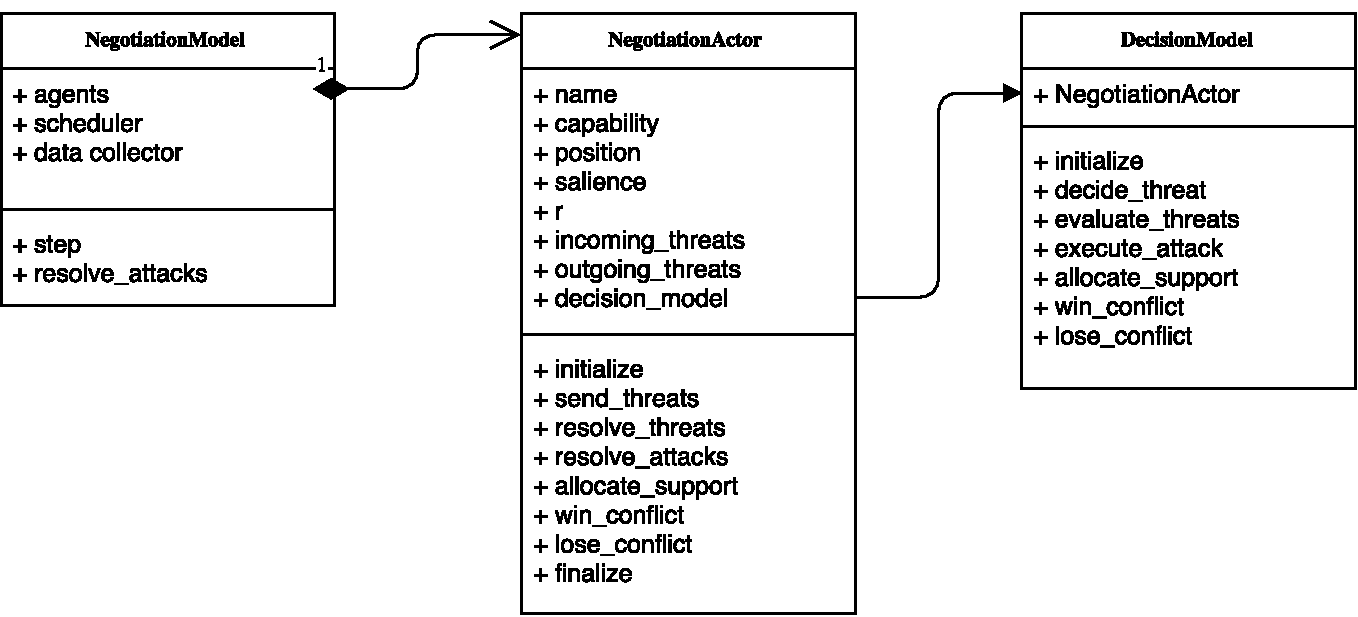
\includegraphics[width=\textwidth]{BDM_Reproduction/Figures/BDM_Architecture}
  \caption{Model Architecture}
  \label{fig:bdm_architecture}
  \figSpace
\end{figure}

\subsection{Details} \label{details}

\subsubsection{Initialization and Inputs} \label{initialization}

Each model instantiation is meant to simulate a particular issue under contention. Thus, we begin by identifying the issue of interest, and the actors we need to represent. In some cases, identifying the actors is simple: for example, all the states who are party to a particular formal negotiation process, or (in a retrospective simulation) all the states who participated in a particular conflict. In other cases, qualitative expertise (the modeler's own, or elicited from subject-matter experts) may be needed to determine who the relevant actors are.

For every actor, we must assign position, salience, and capability values. Like the list of actors, the actor properties may be derived from different sources. We may elicit subject-matter experts for their estimates, or utilize various quantitative datasets more objective or replicable measures. Capabilities are perhaps the easiest to measure objectively; the National Material Capabilities (NMC) dataset \citep{singer_1972,singer_1988} provides several calibrated measures of national power, aggregated into the Composite Index of National Capability (CINC). Position is harder to measure. One method is computing the similarity of states' alliance portfolios \citep{bdm_1975,bdm_1992,signorino_1999b}: the more similar the alliances that two states hold are, the closer their interests are presumed to align. There has not been, to the best of my knowledge, an attempt to formally estimate salience from data. It can either be set based on expert estimates, or treated as an unobserved random variable.

%% Submodels

\subsubsection{Risk Propensity Update ($\mathbf{R_0}$)} \label{risk_update}

Conceptually, actors wish to balance between their preferred issue outcome and their desire to be a part of a winning coalition. At one extreme, an actor may adhere to its own position regardless of the positions of the rest of the actors, and no matter how much power is arrayed against it. At the other extreme, an actor may completely abandon its preferred position and seek to position itself as close as possible to the current consensus or winning position. In practice, most actors are likely to fall somewhere between these two poles.

In order to estimate each actor's risk propensity, the model compares the actor's current security to the security of all other actors in the model. More formally:

\begin{equation}
    R_i = \frac{ 2 \sum\limits_j E^i(U_{ji}) - \max\limits_j \sum\limits_{k} E^i(U_{kj})  -  \min\limits_j \sum\limits_{k} E^i(U_{kj})}{\max\limits_j \sum\limits_{k} E^i(U_{kj})  -  \min\limits_j \sum\limits_{k} E^i(U_{kj})} \label{eq:R_0}
\end{equation}

In this equation, $E^i(U_{ji})$ refers to agent $i$'s perception of $j$'s expected utility of threatening $i$; the full expected utility calculation is specified in Equation \ref{eq:EU}. This result is then normalized as follows:

\begin{equation}
    r_i = \frac{1 - R_i/3}{1 + R_i/3}
\end{equation}

In the model as described in \citet{bdm_2002} and \citet{scholz_2011}, the risk propensity is recalculated at every step, with an initial assumption of $r_i=1$ for all actors. This means that risk propensity is not a fixed property of the actor, but emerges from the overall model state. This can be thought of as the risk propensity required to maintain the actor's current position.

\subsubsection{Expected Utility Calculation ($\mathbf{O_0}$)} \label{eu_calc}

The expected utility (EU) calculation is important enough to have given the model the name it is most often known as -- the Expected Utility Model. In each step of the model, the first decision facing each agent is whether to send an offer to each other agent, which they will do only if their expected utility is positive.

In order to compute the expected utility of threatening a particular target $j$, actor $i$ computes the utilities of the following potential outcomes:

\begin{enumerate}
    \item The actor threatens the target, and:

        \begin{enumerate}
        \item Enters into conflict and wins: 
            \begin{equation}
            U_s = 2 - 4(0.5 - 0.5|x_i - x_j|)^{r_i} \label{eq:u_s}
            \end{equation}
        \item Enters into conflict and loses:
            \begin{equation}
            U_f = 2 - 4(0.5 + 0.5|x_i - x_j|)^{r_i}
            \end{equation}
        \item The target capitulates without a conflict ($U_s$ again, as computed in Equation \ref{eq:u_s})
        \end{enumerate}
    \item The actor does not threaten the target, and:
        \begin{enumerate}
        \item The status quo continues:
            \begin{equation}
            U_{sq} = 2 - 4(0.5)^{r_i}
            \end{equation}
        \item The target moves towards the current median position $\mu$:
        \begin{equation}
            U_b = 2 - 4(0.5 - 0.25(|x_i-\mu|+|x_j-\mu|))^{r_i}
            \end{equation}
        \item The target moves away from the current median position $\mu$:
        \begin{equation}
            U_w = 2 - 4(0.5 + 0.25(|x_i-\mu|+|x_j-\mu|))^{r_i} \label{eq:u_w}
            \end{equation}
        \end{enumerate}
\end{enumerate}

Next, the actor assigns probabilities to each outcome. The probability of winning and losing the conflict are this actor's perception of the fraction of support allocated to its position as compared to the target's. For a conflict between agents $j$ and $k$, actor $i$'s support (or `votes') is computed as follows:

\begin{equation}
    v^{i}_{jk} = c_is_i (|x_i-x_k| - |x_i-x_j|) \label{eq:votes}
\end{equation}

When $v^{i}_{jk}$ is positive, $i$ supports $j$; negative, and $i$ supports $k$. In light of this, $i$'s perceived probability of a victory by $j$ in a conflict between $j$ and $k$ is:

\begin{equation}
P^i_{jk} = \frac{\sum\limits_{h|v^h_{jk}>0}v^h_{jk}}{\sum\limits_{h}|v^h_{jk}|} \label{eq:p_win}
\end{equation}

This probability calculation is also used to determine the median position. The model extends the \citet{black_1948} median voter calculation to account for the fact that each actor has a different `voting' power, and may cast a different number of votes (allocate a different level of support) in different bilateral contests. The median position $x^*$ is thus:

\begin{equation}
    x_i^* \equiv P^i_{*k} > 0.5 \text{ } \forall \text{ } k \in N
\end{equation}

Or, plainly, the position which is likely to defeat all other positions in bilateral contests.

The target's salience is used as the probability that it will yield to the threat, rather than enter into a conflict. Finally, the actor's perception of the probability of the target not moving at all is denoted $Q_i$; and of the target moving towards the median position if it does move is $T_i$. These appear to generally be held fixed for all agents in a given model instantiation, and as such become model parameters. 

Putting all the terms together gives us the full expected utility calculation. For convenience, the equation below omits all the full perception designation terms. The utilities are $i$'s perception of $j$'s utility of winning, losing, etc. $P$ is $i$'s perception of $j$'s probability of winning the conflict. 

\begin{equation}
    \label{eq:EU}
    \begin{split}
    E^i(j,k) = E^i(U_{jk}) = s_k (P U_s + (1-P)U_f) + (1 - s_k)U_s \\
    - Q_i U_{sq} + (1-Q_i)(T_iU_b + (1-T_i)U_w)
    \end{split}
\end{equation}

This EU value comes into play in several ways: first, at each step, agents issue an offer when the expected utility is positive -- that is, the agents expect a better outcome from issuing a threat than not issuing it. Second, it determines how each target of a offer responds, as the next section describes.

\subsubsection{Responding to Offers ($\mathbf{M_0, A_0}$)} \label{challenges}

Once all the actors have sent their offers, they decide on at most one offer to accept. The offer selection mechanism is perhaps the least specified of all the model components in any of the prior literature. I utilize the description provided by \citet{scholz_2011}, who argue that agents choose offers based on two criteria: the expected utility associated with each offer, and the distance it requires the target actor to move.

In this approach, agents initially evaluate the distance between their current position, and the position associated with the offer. Agents will choose offers where this distance is the smallest, preferring to accept offers requiring them to change position the least.

If there is a single closest offer, it is selected. However, if there are multiple offers with the same distance associated with them, the agent selects the most enforceable one -- that is, the one with the highest perceived expected utility on the part of the sender.

How agents actually change their position based on their accepted offer is determined by the combination of the source and the target's expected utility of threatening one another. In other words, this can be thought of as both actor's expected utility from a conflict, and how much does each stand to gain or lose in that case. Specifically, there are several octants based on these utilities, as shown in Figure \ref{fig:octants}.

\begin{figure}
  \centering
  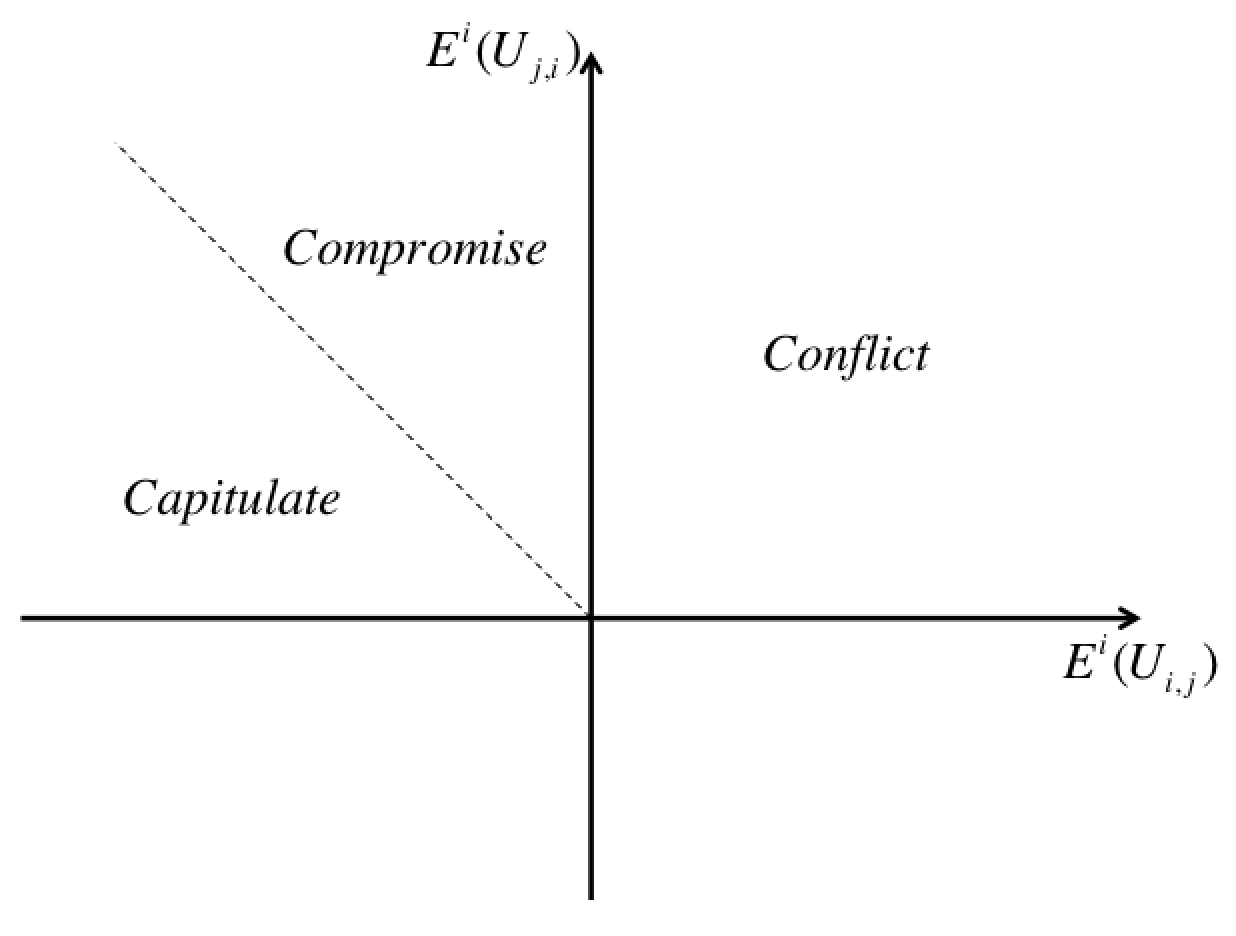
\includegraphics[scale=0.5]{BDM_Reproduction/Figures/Octants}
  \caption{Incoming Offer Categories}
  \label{fig:octants}
  \figSpace
\end{figure}

\begin{description}
    \item[Capitulate:] This octant is the region of the EUxEU space where the target's EU is negative, and has an absolute value greater than the positive EU of the source. More colloquially, the target stands to lose more than the attacker stands to gain. This indicates a decisive advantage for the source in case of a conflict; in the face of some advantage, the target yields completely, adopting the source's position as its own. 

    \item[Compromise:] In this octant, the target's EU is negative, but smaller in magnitude than the source's. In this case, the sender cannot enforce complete surrender, but can nevertheless coerce the target into changing its position towards that of the sender. The size of the step is determined by the ratio between the magnitudes of both actors' expected utilities, or more formally:
    
    \begin{equation}
        x_i^\prime = x_i + (x_j - x_i)\left\lvert\frac{E^i(U_{ji})}{E^i(U_{ij})}\right\rvert
    \end{equation}

    Thus, as the source's EU increases, the target agrees to increasingly better compromises.

    \item[Conflict:] The conflict quadrant consists of the region of the space where both actors' expected utility from a conflict is positive; in other words, conflict can occur only when both actors expect to gain from it. When actors choose to enter into a conflict with one another, the Conflict sub-model is called, as described below.

\end{description}

\citet{bdm_2002} notes that ``Each player is free to renege on a proposed deal so long as it can enforce another agreement or so long as someone else can enforce an agreement on it.'' In practice, the latter part of the sentence refers to the fact that actors choose only one incoming offer to accept; I interpret the first half to mean that actors need not change position if another actor accepted their offer and is changing position towards them. This resolves a situation I observed while developing and experimenting with the model, where actor A capitulated to actor B, while actor B simultaneously capitulated to actor C -- in effect, B coerces A into holding a position A itself is simultaneously abandoning.

\subsubsection{Conflicts ($\mathbf{W_0}$)}

Conflicts occur when both actors see positive expected utility from a conflict with the other, leading them to choose each other's offer, and when neither agent reneges due to another agent accepting their offer. For each conflict occurring in a given step, all agents contribute some fraction of their capabilities to one side or the other, as described in Equation \ref{eq:votes}, yielding the probability given in Equation \ref{eq:p_win}. The model stochastically chooses the winner with that probability, and the loser updates their position to that of the winner. The assumptions regarding conflicts are discussed in much more detail in Section \ref{bdm_discussion}.

\section{Model Validation and Verification} \label{model_vv}

The description above appears, to the best of my ability to ascertain, to be a faithful representation of the BDM Expected Utility model, as presented in the prior literature. However, as documented by \citet{scholz_2011}, not only has the model never been fully specified, but several components of it have been modified over time. In this section, I attempt to validate my implementation against two sets of inputs and outputs from the prior literature -- and I should note up-front that in neither of these cases do I successfully fully reproduce the original reported results. In light of this, I conduct a deep dive into one of the model runs and provide a detailed walk-through of a single model step. This serves to verify that the model is working as expected, as well as to build the reader's intuition and understanding of the model's behavior and dynamics.

\subsection{Reproduction of Prior Results} \label{verification}

A natural way to validate that the model described here successfully replicates the original is by reproducing prior results from known inputs. There are several models where the inputs are fully specified (or very nearly so) to allow for such replication attempts. For example, \citet{scholz_2011} uses the data from \citet{bdm_1994}, an application of the model to European vehicle standard negotiations, and demonstrate the reproduction of several model outputs. I attempt to reproduce this replication, and to also the China democratization example examined in \citet[chapter 6]{bdm_2002}. Since the latter model in particular involves a stochastic element, we cannot reproduce the exact same results without knowing outcomes of the various random draws; instead, I examine the distribution of results across multiple model runs. 

The case examined by \citet{scholz_2011} provides a good starting point, since there is minimal stochasticity in the model implementation. The \citet{scholz_2011} replication is validated in two ways: by comparing the median position, and the quadrants pairs of agents fall in, to those produced by the original model. The \citet{scholz_2011} model perfectly reproduces the median position changes reported in \citet{bdm_1994}. Figure \ref{fig:model_comparison}, compares those median positions to those generated by my own implementation. The comparison highlights the fact that the original model produces cyclic behavior which mine does not: certainly a richer dynamic, but not one with any external reason for us to believe it to be correct. (The observed historic outcome, 8.833 years, corresponds to approximately 0.8 on the normalized issue space, which neither model converges to).

\begin{figure}
  \centering
  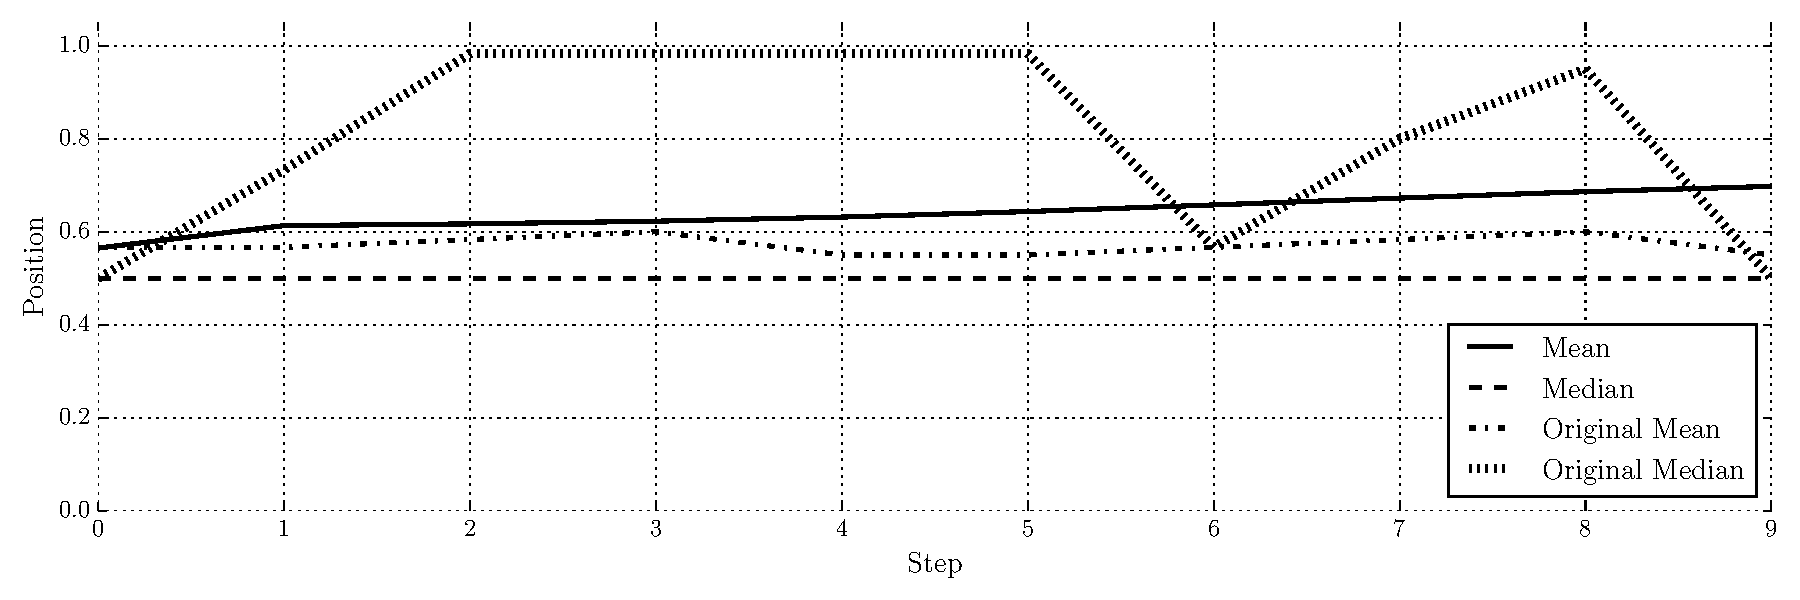
\includegraphics[scale=0.5]{BDM_Reproduction/Figures/ModelComparison}
  \caption{Original and Replication Model Comparison}
  \label{fig:model_comparison}

  \figSpace
\end{figure}

Stronger evidence still that the \citet{scholz_2011} model replicates the BDM results comes from the octant comparison, comparing the expected utilities of between pairs of agents at the first step of the model. As the paper notes, there is a vanishingly-small probability of the same octant configuration resulting by chance. My own model does not replicate these octant configurations. One example is shown in Figure \ref{fig:octant_comparison}, with Belgium as the focal actor -- the position of each other agent is Belgium's expected utility from challenging it, and its own expected utility from challenging Belgium.

\begin{figure}
    \centering
    \begin{subfigure}{0.32\textwidth}
        %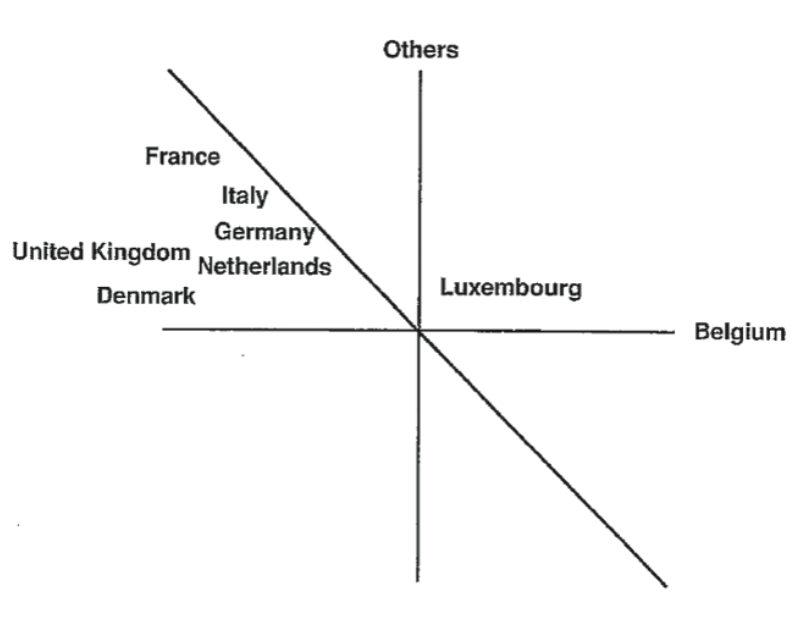
\includegraphics[width=\textwidth]{BDM_Reproduction/Figures/Octants_BDM94}
        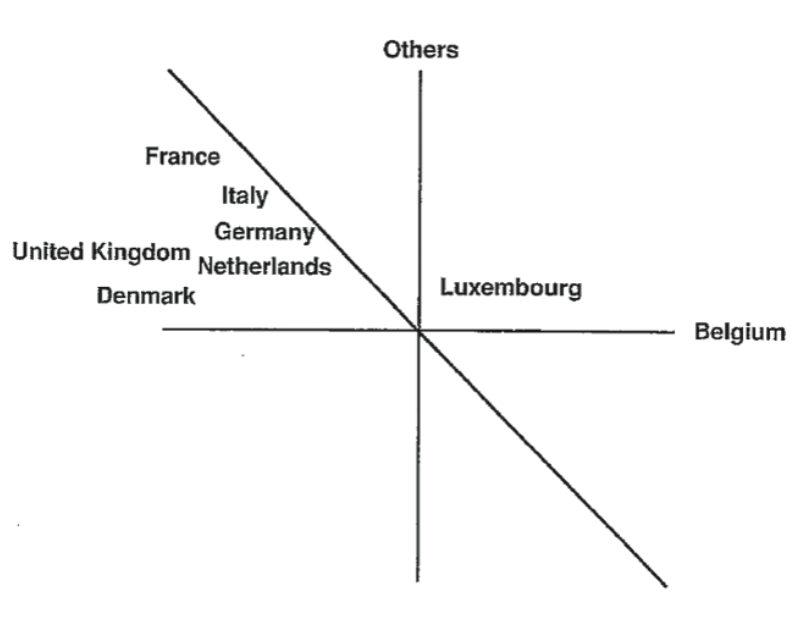
\includegraphics[height=5cm]{BDM_Reproduction/Figures/Octants_BDM94}
        \caption{\citet{bdm_1994} Expected Utilities}
    \end{subfigure}
    \begin{subfigure}{0.32\textwidth}
        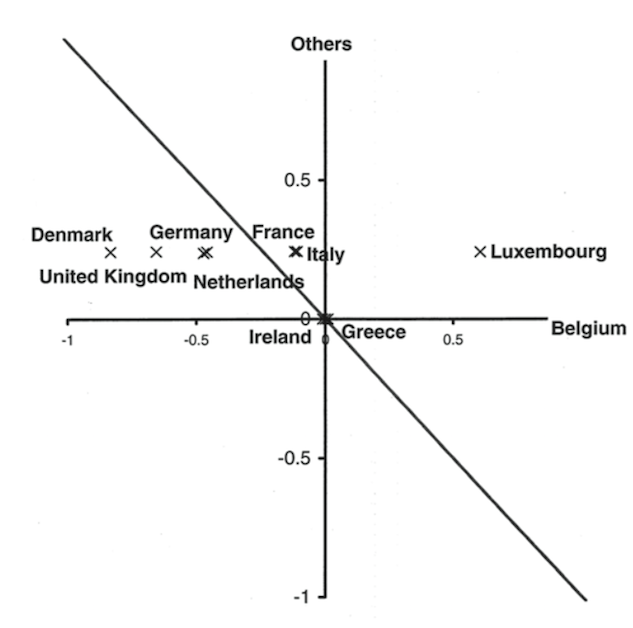
\includegraphics[height=5cm]{BDM_Reproduction/Figures/Octants_Scholz11}
        \caption{\citet{scholz_2011} Expected Utilities}
    \end{subfigure}
    \begin{subfigure}{0.32\textwidth}
        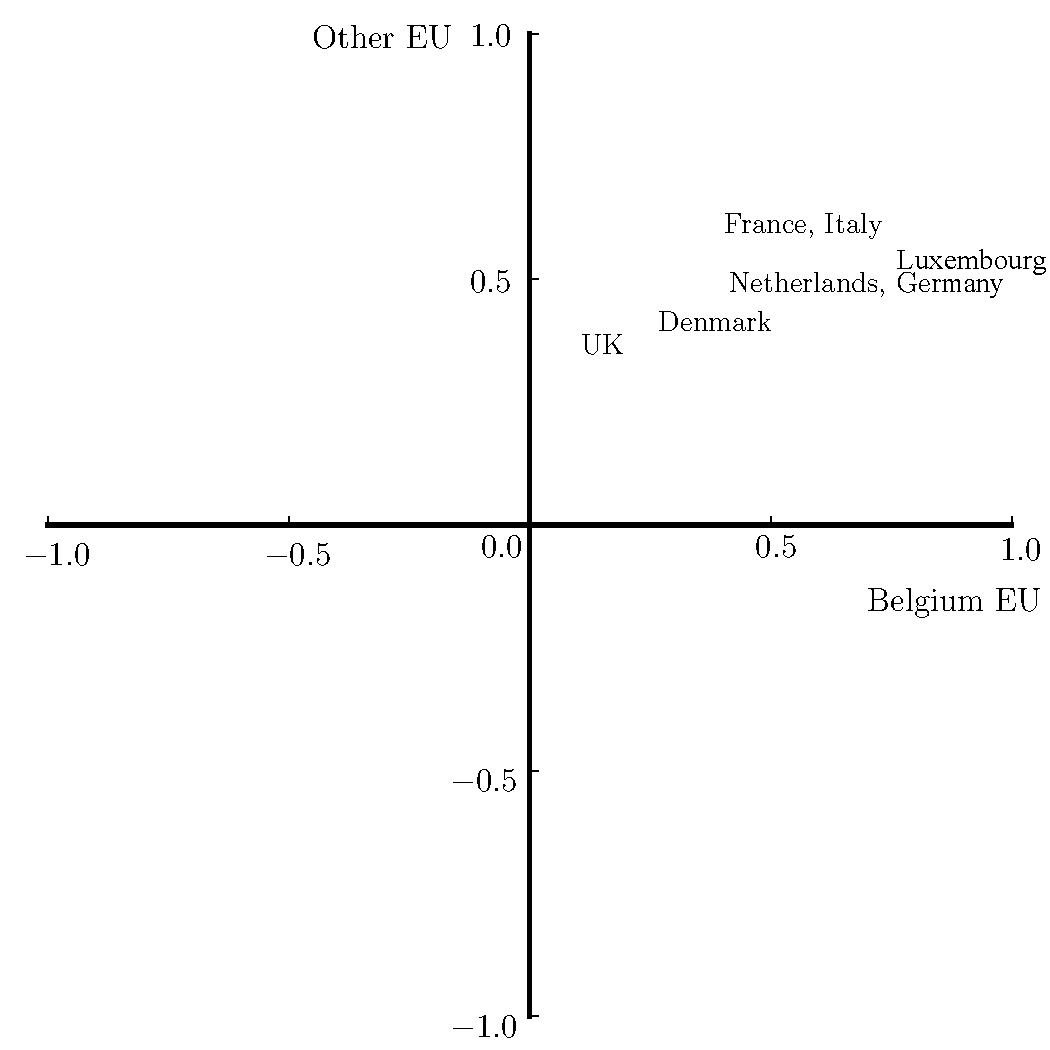
\includegraphics[height=5cm]{BDM_Reproduction/Figures/OctantComparison}
        \caption{Model reimplementation}
    \end{subfigure}

    \caption[Octant Comparison]{Octant Comparison, with Belgium as Focal Agent}
    \label{fig:octant_comparison}
    \figSpace

\end{figure}

A close comparison of the models suggests that the Scholz octant configuration is driven by far smaller probabilities of victory that the model produces, normalized by all possible votes rather than just the ones on the conflict at hand. This probability form appears to contradict the form of probability calculations provided in \citet{bdm_1997,bdm_2002}, and (more importantly) a basic rule of probability: if there are two possible outcomes (in this case, actor $i$ wins or actor $j$ wins), their probabilities must sum to 1. There are, then, two alternatives: one is that the Scholz model is successfully replicating an erroneous BDM model implementation; the other is that there is some other mismatch between the models which is producing matching octants. There are two, somewhat contradictory, preliminary conclusions we can take from here: that the overall model is sensitive to changes in specific sub-models, and that it is nevertheless robust enough to produce similar results even when these sub-models differ, and produce substantively different interactions.

Furthermore, while the Scholz model successfully replicates specific features of this one particular model instantiation, this success does not translate to other cases. Scholz et al. note that their implementation fails to replicate another case, presented in \citet{bdm_1997}. Experiments on my part confirm that it also fails to replicate the following cases, which I will describe next.

The next case I use is the Chinese democratization example, presented in chapters 3 and 6 of \citet{bdm_2002}. In this case, the model is being instantiated is attempting to predict the dynamics of internal political reform in the People's Republic of China. The agents here are a mix of individuals, organizations, loose factions (e.g. ``Students and Intellectuals''), and foreign countries. \citet{bdm_2002} reports model median positions by step for several model instantiation. However, as part of this particular case, agents' saliences are randomized each step, with 20\% probability each; the reported results do not specify which saliences were changed and how. This makes it effectively impossible to attempt to replicate the exact same model run. To overcome this, I generate many more model runs: 50 of the Scholz model, and 100 of my own. I start each run with the initial conditions provided in \citet{bdm_2002}, and randomize agent salience values as described. This yields a distribution of models, and in particular a distribution of medians. Figure \ref{fig:china_medians} shows the distributions of these medians, as well as a dotted line indicating the reported median\footnote{This median value was taken from \citet[chapter 3]{bdm_2002}; chapter 6 provides only a chart of medians from several runs, but not precise values. However, the chart shows values close to the one used here.}. In this case, the models produce similar, though not identical, distributions to one another -- and neither comes close to the reported values. This indicates that the Scholz model is not a perfect implementation of the original model as implemented. Furthermore, it suggests that we may need to be cautious about using any single set of reported model results as `ground truth.'

In light of these results, and of the reported changes in the variations of the original model, I believe that validating the model reimplementation directly against reported model outputs is not a tenable option. Nevertheless, I believe that the model I have implemented correctly captures the core sub-models of the original, and provides a sufficiently solid basis to proceed with this analysis.

\begin{figure}
    \centering
    \begin{subfigure}{0.49\textwidth}
        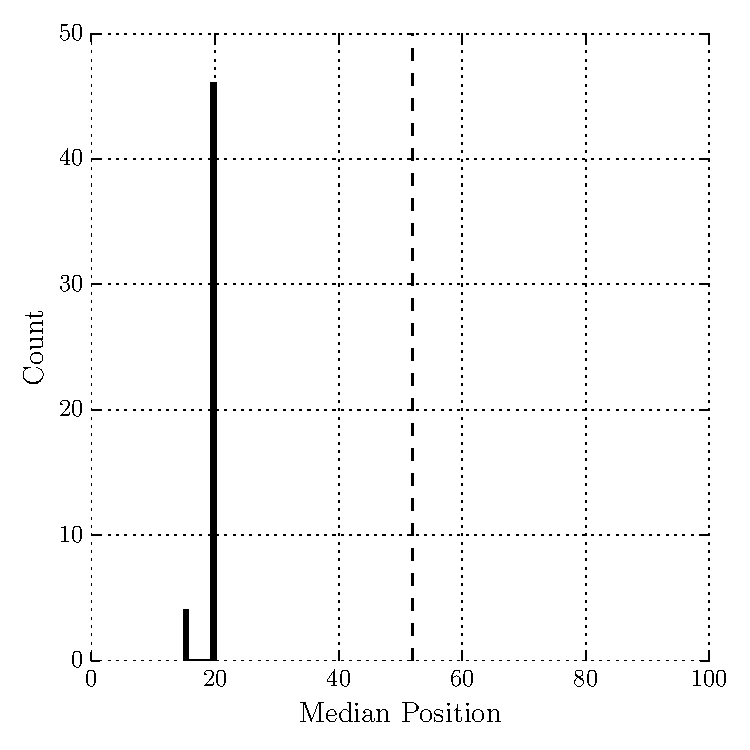
\includegraphics[width=\textwidth]{BDM_Reproduction/Figures/Scholz_ChinaModel}
        \caption{\citet{scholz_2011} Median Positions}
    \end{subfigure}
    \begin{subfigure}{0.49\textwidth}
        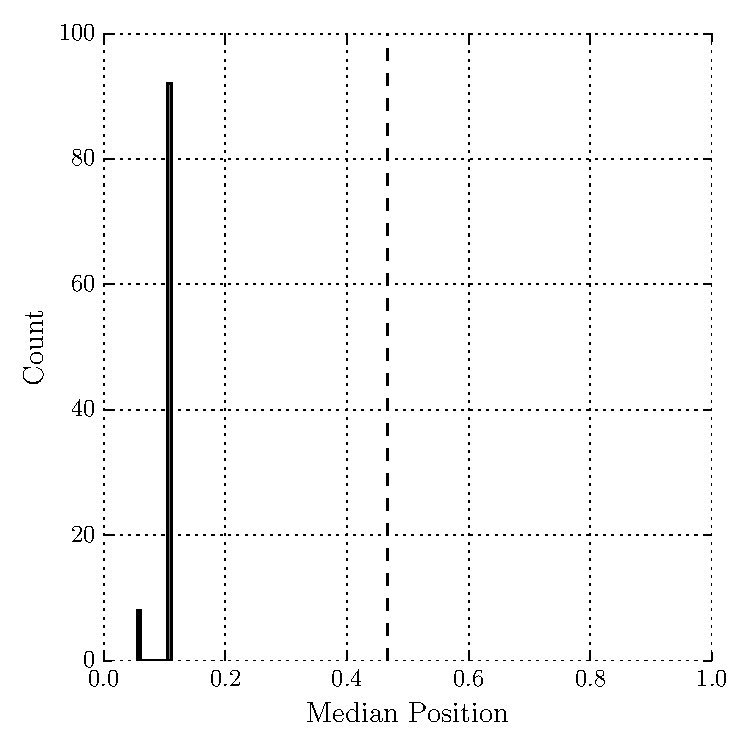
\includegraphics[width=\textwidth]{BDM_Reproduction/Figures/New_ChinaModel}
        \caption{Reimplemented Model Median Positions}
    \end{subfigure}

    \caption[Chinese Democratization Model Medians]{Chinese Democratization Model Medians, at the End of Step 2}
    \label{fig:china_medians}
    \figSpace
\end{figure}


\subsection{Deep Dive} \label{deep-dive}

In order to understand how the model behaves, it is valuable to take a close look at the sequence of actions in a single iteration. This will also serve as a method of verification, ensuring that the model is not producing unexpected or incorrect behaviors. In order to do so, I will continue to use the European vehicle standards model presented above. I choose this example in particular since it has already been well-studied: first by \citet{bdm_1994} directly, then by \citet{scholz_2011} as the key case for testing their replication of the original BDM model; and finally by \citet{mckibben_sanders_2014} testing the replication of the replication. Furthermore, the number of agents is small enough to make the interactions amenable to direct human examination. In this case, the agents are ten members of the European Community (the precursor to the European Union), negotiating over when to apply new emission regulations to mid-size automobiles. This gives the position space a straightforward, numeric interpretation: the years before the regulations are applied. The agent initial positions, capability and saliences were all determined by consultation with subject-matter experts.

\begin{table}
\centering
\caption{Example Model -- Agent Data}
\label{table:eg_agent_data}
\begin{tabular}{lccc|c}
    \hline
    Name &  Capability &  Position &  Salience & $r_{i,t=0}$ \\
    \hline
    Netherlands &        0.08 &       0.0 &       0.8 & 1.12 \\
        Belgium &        0.08 &       0.5 &       0.4 & 1.00 \\
     Luxembourg &        0.03 &       0.0 &       0.2 & 0.50 \\
        Germany &        0.16 &       0.0 &       0.8 & 1.12 \\
         France &        0.16 &       1.0 &       0.6 & 1.02 \\
          Italy &        0.16 &       1.0 &       0.6 & 1.02 \\
             UK &        0.16 &       1.0 &       0.9 & 2.00 \\
        Ireland &        0.05 &       0.5 &       0.1 & 0.65 \\
        Denmark &        0.05 &       0.0 &       1.0 & 1.45 \\
         Greece &        0.08 &       0.5 &       0.7 & 1.56 \\
    \hline
\end{tabular}
\tableSpace
\end{table}

Initially, the model computes the risk propensity coefficients shown in Table \ref{table:eg_agent_data}. Note that indeed one agent, the UK, has a value of $r=2.0$ and another one, Luxembourg, has $r=0.5$; as agents are computing their risk propensity in comparison with one another, this will always be the case.

Next, the agents estimate their expected utility of threatening all other agents, sending offers where those expected utilities are greater than zero. These EUs are given in Table \ref{table:eg_eu}. The important thing to note here is that the majority of directed dyads have a positive EU -- which means that all those dyads will have threats issued across them. 

\begin{table}
\centering
    \caption[Example Model -- Expected Utilities]{Example Model -- Expected Utilities, $t=0$}
    \label{table:eg_eu}
    \begin{tabular}{r|cccccccccc}

        Source  \textbackslash Target &  Bel. &  Den. &  Fra. &  Ger. &  Gre. &  Ire. &  Ita. &  Lux. &  Net. &    UK \\
        \hline
        Belgium     &      -- &     0.27 &    0.40 &     0.41 &    0.00 &     0.00 &   0.40 &        0.85 &         0.41 &  0.11 \\
        Denmark     &     0.39 &      -- &    0.08 &     0.00 &   -0.00 &     0.79 &   0.08 &        0.00 &         0.00 & -0.61 \\
        France      &     0.60 &     0.28 &     -- &     0.62 &    0.29 &     0.90 &   0.00 &        1.64 &         0.62 &  0.00 \\
        Germany     &     0.47 &     0.00 &    0.46 &      -- &    0.08 &     0.86 &   0.46 &        0.00 &         0.00 & -0.23 \\
        Greece      &     0.00 &     0.13 &    0.27 &     0.28 &     -- &     0.00 &   0.27 &        0.74 &         0.28 & -0.04 \\
        Ireland     &     0.00 &     0.30 &    0.42 &     0.43 &    0.00 &      -- &   0.42 &        0.80 &         0.43 &  0.17 \\
        Italy       &     0.60 &     0.28 &    0.00 &     0.62 &    0.29 &     0.90 &    -- &        1.64 &         0.62 &  0.00 \\
        Luxembourg  &     0.46 &     0.00 &    1.45 &     0.00 &    0.18 &     0.74 &   1.45 &         -- &         0.00 &  0.76 \\
        Netherlands &     0.47 &     0.00 &    0.46 &     0.00 &    0.08 &     0.86 &   0.46 &        0.00 &          -- & -0.23 \\
        UK          &     0.35 &    -0.70 &    0.00 &    -0.36 &    0.04 &     0.65 &   0.00 &        0.66 &        -0.36 &   -- \\
    \end{tabular}
    \tableSpace
\end{table}

\begin{table}
\centering
    \caption{Accepted Offers}
    \label{eg_offers}
\begin{tabular}{lll}
    \hline
    Agent &  Accepted Offer & Category \\
    \hline
    Netherlands & Belgium & conflict \\
    Belgium & Netherlands & conflict \\
    Luxembourg & Belgium & conflict \\
    Germany & Belgium & conflict \\
    France & Belgium & conflict \\
    Italy & Belgium & conflict \\
    Ireland & Netherlands & conflict \\
    Denmark & Greece & compromise \\
    Greece & UK & compromise \\
    \hline
\end{tabular}
\tableSpace

\end{table}

Table \ref{eg_offers} shows which offer each agent accepts, and what category each one falls into. Immediately, we notice that five agents all choose to enter into conflict with Belgium. Note that Belgium's position is exactly in the middle of the issue space, and it has lower salience than Greece, the other agent holding the same position, making it an appealing target. For a conflict to occur, Belgium must choose one of them -- and indeed chooses the Netherlands, which leads to a conflict. Meanwhile, Denmark chooses to compromise with Greece and update its position towards it, while Greece chooses to compromise with the UK. However, recall that agents renege on offers if another agent has accepted their own offer in a more preferable way. In this case, since Denmark has chosen to compromise with Greece, Greece in turn backs out from its decision to compromise with the UK, and will not update its position at all.

The conflict between Belgium and the Netherlands happens before Denmark updates its position. Each agent contributes capability to one side or the other, as governed by Equation \ref{eq:votes}; these contributions are shown in Table \ref{table:contributions}. Note that even the two actual actors entering into the conflict do not allocate their full capabilities: they are scaled once by their salience, and again by the distance between their positions. Putting the total values into Equation \ref{eq:p_win} yields a probability of victory of 0.63 for Belgium, and thus 0.37 for the Netherlands. The model uses these probabilities to randomly select the winner; if Belgium wins, the Netherlands updates its position to 0.5, and if the Netherlands wins Belgium updates its own position to 0. At this point, Denmark will update its own position to compromise with Greece. Then, the next round begins.

\begin{table}[h!]
\centering
    \caption{Capability Contribution -- Belgium vs Netherlands}
    \label{table:contributions}
\begin{tabular}{lcc}
    \hline
    Agent &  Belgium & Netherlands \\
    \hline
    Netherlands & 0 & 0.032 \\
    Belgium & 0.016 & 0 \\
    Luxembourg & 0 & 0.003 \\
    Germany & 0 & 0.064 \\
    France & 0.048 & 0 \\
    Italy & 0.048 & 0 \\
    UK & 0.072 & 0 \\
    Ireland & 0.0025 & 0 \\
    Denmark & 0 & 0.025 \\
    Greece & 0.028 & 0 \\
    \textbf{Total} & \textbf{0.2145} & \textbf{0.124} \\
    \hline
\end{tabular}
\tableSpace

\end{table}

%Table \ref{eg_offers} shows which offer each agent accepts, and what category each one falls into. Immediately, we notice that six agents all choose to enter into conflict with Belgium. Note that Belgium's position is exactly in the middle of the issue space, and it has lower salience than Greece, the other agent holding the same position, making it an appealing target. For a conflict to occur, Belgium must choose one of them -- and indeed chooses the Netherlands, which should lead to a conflict. However, recall that agents renege on offers if another agent has accepted their own offer in a more preferable way. In this case, Denmark agrees to compromise with Belgium, meaning that Belgium will in turn back out of its conflict with the Netherlands. In the end, in fact, no conflicts occur, and the only movement is by agents moving unilaterally: Greece, capitulating, and Denmark, compromising.

\section{Model Discussion} \label{bdm_discussion}

Examining the description of the model above, we can see clearly that it is in fact an agent-based model: the actors are agents, interacting with each other in discrete steps according to a set structure. Each agent is endowed with several properties, some public and some private, making it natural to model them using object-oriented design. Indeed, the focus on the utility calculations in much of the prior literature elides the deeply computational nature of this model. It is anchored not only in game-theoretic logic, but on embedded assumptions which have a substantial effect on the model's behavior, and which, when articulated in code, are easy to experiment with. 

The model, like many agent-based models, can be separated into two layers: the agents' external behavior with regard to one another, and their internal decisionmaking process. 

Externally, agents send threats to some other agent. A threat has no information specifically attached (though of course the target has access to the public information on the source of the threat) -- it is simply boolean; either a source has issued a threat to a target, or it has not. Next, all agents choose how to change their public positions in response to the incoming threats -- and these choices are public, and simultaneously become common knowledge. When two agents have chosen conflict with one another, conflicts occur and are resolved. Finally, agents update their stated positions based on the offers and conflict outcomes, before the sequence starts over. These steps happen in sequence with one another, but that all agents act simultaneously within each step.

Note that at no point in this sequence do utilities, expected or otherwise, come into play. The utilities are computed, and applied, internally by agents to drive their decisionmaking, choosing who to send threats to and how to respond to them. We can easily imagine other beliefs and heuristics guiding agent decisions besides the ones that have been chosen here. Even the sequence of events itself is not necessarily fixed.

In this section, I will discuss several of the model assumptions in greater depth. I also propose sub-model variants which implement alternative assumptions. The object-oriented nature of the model means that a single sub-model to be replaced without modifying any other aspect of it. This, in turn, allows us to instantiate different model variants with the same initial conditions and directly compare their dynamics and outputs -- and, in turn, use these to understand how the assumptions drive the model as a whole.

\subsection{Expected Utility}

While the expected utility calculation (Equation \ref{eq:EU}) is important enough to give the model its name, I note that this calculation is largely heuristic in nature. The probability of winning or losing $P$ (as computed in Equation \ref{eq:p_win}) is based on the best possible approximation. The inclusion of the salience term as a probability, however, is much more obviously a heuristic. The source of a potential threat uses salience as the probability of the target yielding to that threat. However, salience does not play a similar role in the threat response side of the model; in fact, it is possible for an agent to have low salience and high probability of winning a conflict, and hence high EU, due to support from other agents. Simply put: agents are modeled as making an estimation that is plausible on its face, but that nevertheless does not reflect the reality of the model itself. 

$Q$ and $T$ are more clearly broad heuristics: they are not as specifically tied to the behavior of a particular agent, but are approximate, coarse-grained estimates of the behavior of the world overall. While \citet{bdm_2002} suggests that agents update their belief about the world in response to the outcome of each round, no such learning rule is provided. $Q$ and $T$ provide candidates for such updating: for example, the agents could use the fraction of agents that moved last round as $Q$, or update their belief in a Bayesian fashion based on a prior probability distribution for $Q$. Alternatively, we may note that any given model potentially represents one issue among many which the actors are addressing at once or in rapid sequence, and suggest that $Q$ and $T$ represent heuristics developed across all issues.

\subsection{Conflict and Coercion} \label{conflict_coercion}

The Conflict outcome deserves special attention here. Conflict, and especially war, plays an outsize role in the study of international relations, and indeed in world history. Being able to predict the outbreak of conflicts would be a particularly powerful result from this model, particularly as the risk propensity and probability of victory sub-models were originally developed precisely for such predictions \citep{bdm_1985}. For these reasons, it is important to understand precisely when the model predicts conflicts will occur, and how to interpret such predictions.

There are several ways of handling a conflict and its outcome. The method put forward in \citet{scholz_2011} involves comparing both agents' expected utility from the conflict; the winner is the one with the greater EU, and the loser changes position to match the winner's. I believe this approach is incorrect, for several reasons. EU incorporates a specific term for probability of winning, but also the terms for movement absent a threat -- which, if a conflict is actively breaking out, are no longer relevant. Furthermore, if a conflict is already occurring, it is unclear why the salience should continue to have a probability-like effect. The calculation for $P$ (Equation \ref{eq:p_win}) clearly implies that the probability of winning and losing is tied primarily to the total capability brought to bear, not the expected utilities associated with them.

However, these are secondary objections. Changing position is, ultimately, a decision that is internal to an actor. Allowing one agent to directly change another agent's position would breach the division between agents' external actions and internal decisionmaking. This is not how coercion has generally been understood. Coercion, as described by \citet{schelling_1966}, involves one actor presenting another, explicitly or implicitly, with a choice of complying with some demand or facing some punishment. Schelling describes this punishment primarily as  `pain' or `hurt' -- in other words, disutility. Importantly, in this view, the punishment need not degrade the target's capabilities, or eliminate it as a threat; it must simply impose a cost that is greater than the cost of complying with the given demand. Furthermore, if we examine militarized conflicts in particular, only a minority end with one side completely changing its orientation -- for example, the Second World War led to Japan's conversion by force from being an enemy of the United States to its ally \citep{schaller_1997}, and Tanzania's invasion of Uganda in 1978-79 successfully replaced the regime of Idi Amin with one friendly to Tanzania's interests \citep{acheson_2001}. However, in the majority of cases, even if one side has successfully forced concessions from the other (such as in the Falklands or Gulf Wars), the other side's overall geopolitical orientation remains largely unchanged; certainly, they do not become allies of the power which defeated them.

The expected utility calculation, and its role in the model, is compatible with this view. There is an explicit negative utility to losing a conflict, which the agents attempt to avoid. The greater this threat -- the lower the overall expected utility of a conflict -- the more likely the agent is to capitulate entirely. Conflict cannot reduce agents' capabilities, or remove them from the model, suggesting that the disutility of losing bears more resemblance to Schelling's `punishment' than `brute force.' Though the utilities associated with winning and losing a conflict are directly tied to the difference between the agent positions positions, this does not necessarily imply that the agents must change position upon losing. If the cost of losing conflict is solely having one's position changed, what motive do actors in the `Capitulate' octant have to indeed capitulate, rather than embrace a chance, however slight, of changing the source's position through conflict? If a conflict does not change agent positions, it follows that these utilities are exogenous to the utility directly gained by an agent to have support at its current position. And indeed, in general, political actors do gain utility from winning (or succeeding in) a conflict: in the form of increased internal public support, prestige, credibility, and potentially an improved power ratio compared to the loser, while failing at a conflict carries the inverse costs \citep{bratton_2005}. Furthermore, both the means and the stakes of conflict will not be the same for close allies and rivals. Agents may attempt to coerce an ally, but are unlikely to use harsh measures which will risk harming the ally substantially and thus undermining their own position; similarly, the gains from inflicting such lesser costs on an ally will be less than those of inflicting greater losses on an enemy. 

We must note, of course, that the interpretation of conflict varies based on the particular scenario and issue under consideration. In modeling a negotiation over regulatory issues, conflict is highly unlikely to be military. However, in modeling geopolitical contests, conflicts may range from diplomatic snubs to economic sanctions to all-out war. Even military conflicts range in severity. A border clash, or targeted airstrikes, may inflict some costs on the target, but are unlikely to have direct system-wide effects. However, armed conflict between nuclear superpowers, as is a potential outcome in the \citet{bdm_1998} Cold War model, runs the risk of consequences far outside the scope of this model.

Finally, the model elides the difference between when agents decide to engage in conflict and when the conflict, in fact, occurs. An implication of the offer-choice mechanic is that conflict occurs only when both parties choose to engage in it. This seems to remove the possibility of unilateral attacks. Furthermore, both parties to a conflict estimate the capability contribution of all other actors based on the parties' own risk propensity, and the agents' current positions. It seems reasonable that, once a conflict is initiated, other agents actually contribute capability based on their own decision rule -- and in particular, based on their own risk propensity. Here the precise scheduling of the conflicts compared to the rest of the model come into play: if conflicts occur \emph{after} agents change their positions in response to threats, their contribution of resources, and even the side to which they will contribute, may differ from their contributions before moving.

Based on this discussion, I propose two new sub-model variants. As these variants appear better grounded in prior theory than the baseline, I hypothesize they will produce better correspondence with empirical data.

\textbf{Conflict without position changing ($\mathbf{W_1}$):} Under this conflict sub-model variant, agents' positions are not changed when they lose a conflict. 

\textbf{Positions update before conflicts ($\mathbf{T_1}$):} Under this schedule variant, conflicts occur only after agents have moved in response to offers. This means that by the time a conflict occurs, the balance of power has shifted from what it was when the original threat was made.

\textbf{One-way attacks ($\mathbf{A_1}$):} This attack decision model variant removes the requirement for both agents to choose the other's offer for a conflict to be initiated. In this variation, an agent can attack any other agent it had threatened previously in this model step. However, it adds an additional decision-point, before attacks actually occur. At this decision point, the agent evaluates a modified form of the expected utility, which removes the uncertainty factors as to the target's position, since the target's new position is already known.

\begin{equation}
    EU_i^\prime(i,j) = P U_s + (1-P)U_f - U_sq
\end{equation}

Depending on when the agents new positions take effect, $P$, $U_s$ and $U_f$ may all be different from the values calculated at the offer-sending phase. If either the source or the target have changed position, the utilities of victory and defeat will be different as well; furthermore, if other agents have changed position, the direction and magnitude of support they are expected to provide will also have changed, changing the value of $P$ as well.

\subsection{Risk Propensity}

The risk propensity model attempts to estimate the risk an agent is willing to endure in pursuit of a preferred outcome; however, this is not directly risk propensity in the traditional economic sense (i.e. a relationship between a probability and the potential payoff an agent would require to wager on it), but in the political sense: how exposed the agent is willing to be to the possibility of being attacked, or simply left out of a winning coalition, in order to advocate for its preferred position or outcome. \citet{bdm_2002}, citing \citet{lamborn_1991}, describes this as a tradeoff between political satisfaction and policy satisfaction. When an agent is very secure, it is assumed to have chosen that secure position due to a low risk propensity; when it is insecure, this is taken as a revealed higher risk propensity.

Risk propensity is a key place where agents mirror-image: assuming that the other agents will make decisions the same way as they themselves do \citep{heuer_2001}. When agents estimate other agents' expected utility from an offer (Equation \ref{eq:EU}) they do not have access to the other agent's risk propensity, and so use their own instead, as detailed in Equations \ref{eq:u_s}--\ref{eq:u_w}. Mirror-imaging is a well-documented phenomena in humans \citep{meltzoff_2003}, and is also one of the cognitive traps intelligence analysts are frequently warned against \citep{heuer_2001} -- this suggests that it is not an unreasonable assumption for capturing real behavior. Nevertheless, risk propensity in this model is not an inherent property of the agent but emerges from the current configuration of positions. Thus, it is not at all clear whether we ought to expect organizations (or the individuals who compose them) to mirror-image on a dynamic, second-order property.

The form of the risk propensity calculation itself is explicitly grounded in Prospect Theory \citep{kahneman_1984,mcdermott_2001} in that it compares the agent's current security to two framing values: the best and worst possible security values for the agent. This helps explain why this value is recalculated each step: the best and worst security values may well have changed. This is expressed in a more generalized from of Equation \ref{eq:R_0}, using a non-specific security metric:

\begin{equation}
    R_i = \frac{ 2 security_i - \max\limits_j (security_j)  -  \min\limits_j (security_j)}{\max\limits_j (security_j)  -  \min\limits_j (security_j)}
\end{equation}

The original model measures security level as the sum of incoming expected utilities against an agent, or more formally:


\begin{equation}
    security_i = \sum_{j \in N} EU_i(j, i)
\end{equation}

Using this measure, a higher number (worse security) indicates more, and more powerful, potential attacks at the agent's current position.

I propose an alternative security level metric: the summed probabilities of successful attacks. This has the advantage of not relying on other's potential gain and loss; furthermore, unlike EU, probabilities are strictly positive, and thus negative values cannot reduce this value.  This metric was also adopted by \citet{wise_2015a}, as well as by another similar model variant reported to me by private communication. Formally, this security metric is:

\begin{equation}
    security_i = \sum\limits_{j \in N} P_i(j, i) \label{eq:r1_security}
\end{equation}

Next, consider the range of alternatives. In the original, this range is the security levels of all the other agents, or:

\begin{equation}
    \max\limits_{j \in N} (security_j)
\end{equation}

(and likewise for $min$). This method assumes that agents' risk propensities are relative to those of other agents. In particular, it has the consequence that one agent will always have the maximum possible risk propensity, while another will always have the minimum value. The alternative I introduce compares each agent's positions not to those of other agents, but to other possible positions the agent itself could hold, while holding all other agent positions constant. This follows the methodology used in \citet{bdm_1985}, as well as \citet{bdm_1992} and \citet{bennett_2000b}, and appears true to the description in \citet{bdm_2002} of examining ``the most political welfare... and the least the actor could have realized.'' 

\begin{equation}
    \max\limits_{x \in {[0, 1]}} (security_{i|x_i=x}) \label{eq:r1_range}
\end{equation}

This follows from an assumption that if an agent is holding a position which reduces their security they are more risk-accepting, while a position which increases their security indicates less risk propensity. Note, however, that it still cannot distinguish between an actor whose security-maximizing position is due to risk aversion from one which simply has a preference for that position separate from its degree of risk propensity. 

Putting these two variants together, I designate the risk-acceptance updating sub-model which utilizes Equations \ref{eq:r1_security} and \ref{eq:r1_range} as $\mathbf{R_1}$.

\subsection{Offer Selection}

Much like the expected utility calculation itself, the mechanism for offer selection and position updating is also a heuristic. It assumes that agents associate a particular potential position with each incoming offer, and will only select their new position from among those options. Furthermore, the model assumes that agents whose offers are not selected, or whose offers are reneged on, will simply accept this -- even when they have the coercive capability to force the target to change position. Yet this reneging rule has the effect of substantially reducing the frequency of agents actually changing their position.

I experiment with two alternative heuristics which address these issues. The first is simply stated: agents choose offers according to the original rules, but do not renege even if another agent has accepted their own offer. This is sub-model $\mathbf{M_1}$.

One possible interpretation of the reneging rule is that agents are able to renege with the support of their new allies -- the agent or agents who accepted their offer. In order to capture this dynamic explicitly, I implement an additional offer selection heuristic: threat balancing, which I label $\mathbf{M_2}$. In this variant, agents do not choose among their incoming offers directly. Instead, each agent attempts to balance between those threats, so as to maximize the support it will receive in any conflict. For each incoming offer, the agent evaluates its own EU, and estimates that of the sender. The agent selects the offers where the estimated EU is positive, and its own EU is negative -- that is, credible threats from agents it wants to avoid entering into a conflict with. The agent then updates its position by the weighted mean of these offers, where the weights are the absolute value of the agent's (negative) EU from each. Simply put: the agents do not choose a single offer; instead, they respond to all credible threats, in proportion to how threatening they are.

\subsection{Stochasticity and Uncertainty}

The original model is largely deterministic; the only source of uncertainty is in the outcome of conflicts, which (as Section \ref{deep-dive} suggests) are relatively rare. This determinism has been one of the sources of criticism of the model \citep{brandt_2011}, supported by the fact that the stochasticity of conflicts is rarely explicitly spelled out, and by the model outputs frequently being reported as point forecasts rather than distributions. 

The inputs to the model are based on imperfect, uncertain estimates. Elicitation of estimates from subject-matter efforts is often prone to biases \citep{morgan_2014,tetlock_2005}; even absent such biases, careful methodology is required to capture the experts' uncertainty \citep{gill_2013}. This uncertainty is particularly important since it seems highly unlikely that even experts can meaningfully estimate the difference between, for example, an actor having a salience of 0.69 and 0.71. Nor does replacing expert opinion with quantitative sources remove the uncertainty. Positional measures based on alliance networks are only approximate estimates themselves \citep{signorino_1999b}, while the Composite National Material Capabilities dataset \citep{grieg_2010} (used to provide capabilities in several model instantiations) is a linear combination of several different measures, and as such only provides a very coarse-grained estimate of national power. Even such datasets rely primarily on human coders and archival sources, and regularly update their methodology \citep{gibler_2004}, again suggesting that they cannot be taken as certain estimates. Yet given the complexity which characterizes this model (and indeed, agent-based models more generally), it is possible that even small changes to model parameters will lead to radically different outcomes, even if the system is otherwise deterministic. Many of the model's results are reported as point estimates, suggesting certain, deterministic outcomes. This certainty reduces the model's usefulness, however. The uncertainty of the world is a core assumption in forecasting, both political and otherwise. The purpose of a forecasting model is not to eliminate this uncertainty, but to characterize it, place bounds on it, and make predictions in spite of it. A way of reincorporating this uncertainty into the model is by sensitivity analysis: running multiple instantiations of a model while slightly varying different parameters, and recording the results. Such an analysis is conducted and reported in detail below.


Furthermore, even if the model and agent parameters are perfectly accurate, they will not necessarily remain static for the entire timeframe the model is attempting to forecast. The agent's capabilities, saliences, and potentially even positions may all be subject to exogenous changes and shocks due to processes and events outside the scope of the issue being modeled. Such factors may range from regular, long-term differences in growth rates of national GDP or military spending, to unexpected events such as major terrorist attacks or natural disasters which alter actors' priorities and views of the world.

One way to address this is to exogenously and stochastically change agent properties. Salience is the least concrete of the properties, the hardest to estimate, and more likely than capability to undergo exogenous or random changes; thus, it is not surprising that it is the one most likely to be perturbed. Salience updating is the only area where multiple variants are provided within some of the original BDM papers. \citet{bdm_1998} has all agents' saliences determined randomly at the beginning of each step of the model, while the Chinese democratization model in \citet[chapter 6]{bdm_2002} randomizes agents' saliences with a probability of 30\%. I designate the sub-model variant where agent saliences are randomized every step with probability $p$ as $\mathbf{S_{1,p}}$. Similarly, I suggest a model variant $\mathbf{S_2}$ where agent saliences are randomized once at the beginning of a run, and held constant thereafter.

%\subsubsection{Model Characterization}
\section{Sensitivity Analysis} \label{sensitivity-analysis}

As described above, the model is stochastic only in the outcome of conflicts, and is otherwise deterministic. In fact, in much of the literature, model outputs are reported as only point predictions. This makes it unclear whether these point predictions reflect one particular model run, a the modal results, or whether the model is functionally deterministic and converges to the same results across multiple runs. Furthermore, these results do not account for uncertainties in the input data -- which, as I discuss above, may be inaccurate. Finally, observing the model address each case and instantiation separately makes it difficult to identify whether the model has any artifacts or behaviors which tend to emerge independent of the specifics of each case.

In order to address these questions, I conduct a sensitivity analysis using artificial data, as follows. I first generate 100 sets of 10 notional agents each, with the agent properties drawn randomly as shown in Table \ref{table:sa_params}. Each of these will be an artificial study case, which will serve as the basis for a set of model instantiation. 

\begin{table}
\centering
\caption{Experiment Inputs}
\label{table:sa_params}
\begin{tabular}{cl}
    \hline
    Variable &  Value or Distribution\\
    \hline
    $x_i$            &        $\sim Unif(0, 1)$  \\
    $s_i$            &        $\sim Unif(0, 1)$          \\
    $c_i$            &        $\sim Unif(0, 1)$        \\
    $Q_i$            &   $0.5$ \\
    $T_i$            &   $0.5$ \\
    \hline
    Number of agents &        $10$ \\
    Number of steps per run &        $10$ \\
    \hline
\end{tabular}
\tableSpace
\end{table}

I conduct two experiments with this data. With each artificial study case, I create 100 model instantiations for each experiment, and run each for 10 steps before recording the median position at the final step. In Experiment 1, all instantiations of each case are run with the same initial properties; the only source of stochasticity is the outcome of conflicts. In Experiment 2, each instantiation of each case is perturbed slightly. For each parameter $t_i \in$ ($x_i$, $c_i$, $s_i$) for all agents, I perturb the parameter by a small random value:

\begin{equation}
    t_i^\prime = t_i + \epsilon \text{, where } \epsilon \sim \mathcal{N}(0,0.05) \text{ and } t_i^\prime \in {[0,1]} 
\end{equation}

Each experiment then yields 100 sets of 100 outcomes each. Initially, we can simply examine the distributions of these outcomes. Figure \ref{fig:random_medians} shows histograms for the distributions of outcomes (that is, final median positions) for the first nine cases. Since these are instantiated from the same artificial case, we can directly compare the corresponding histograms in the two sub-figures (e.g. the histograms in the top-left corners both come from the same data, likewise the top-center histograms, etc.) Several things are immediately obvious. Several of the cases in Experiment 1 result in a single outcome across the instantiations. Despite the model's stochasticity, these runs all converge to the exact same median outcome. In fact, across all 100 artificial cases, Experiment 1 produces convergent results in 29 of them. This suggests that there are two qualitatively different categories of cases: ones where the model identifies no uncertainty, and ones where it does. In contrast, Experiment 2 produces no convergent results, and shows wider distributions of outcomes even when the corresponding cases in Experiment 1 are not convergent.

\begin{figure}
    \centering
    \begin{subfigure}{0.49\textwidth}
        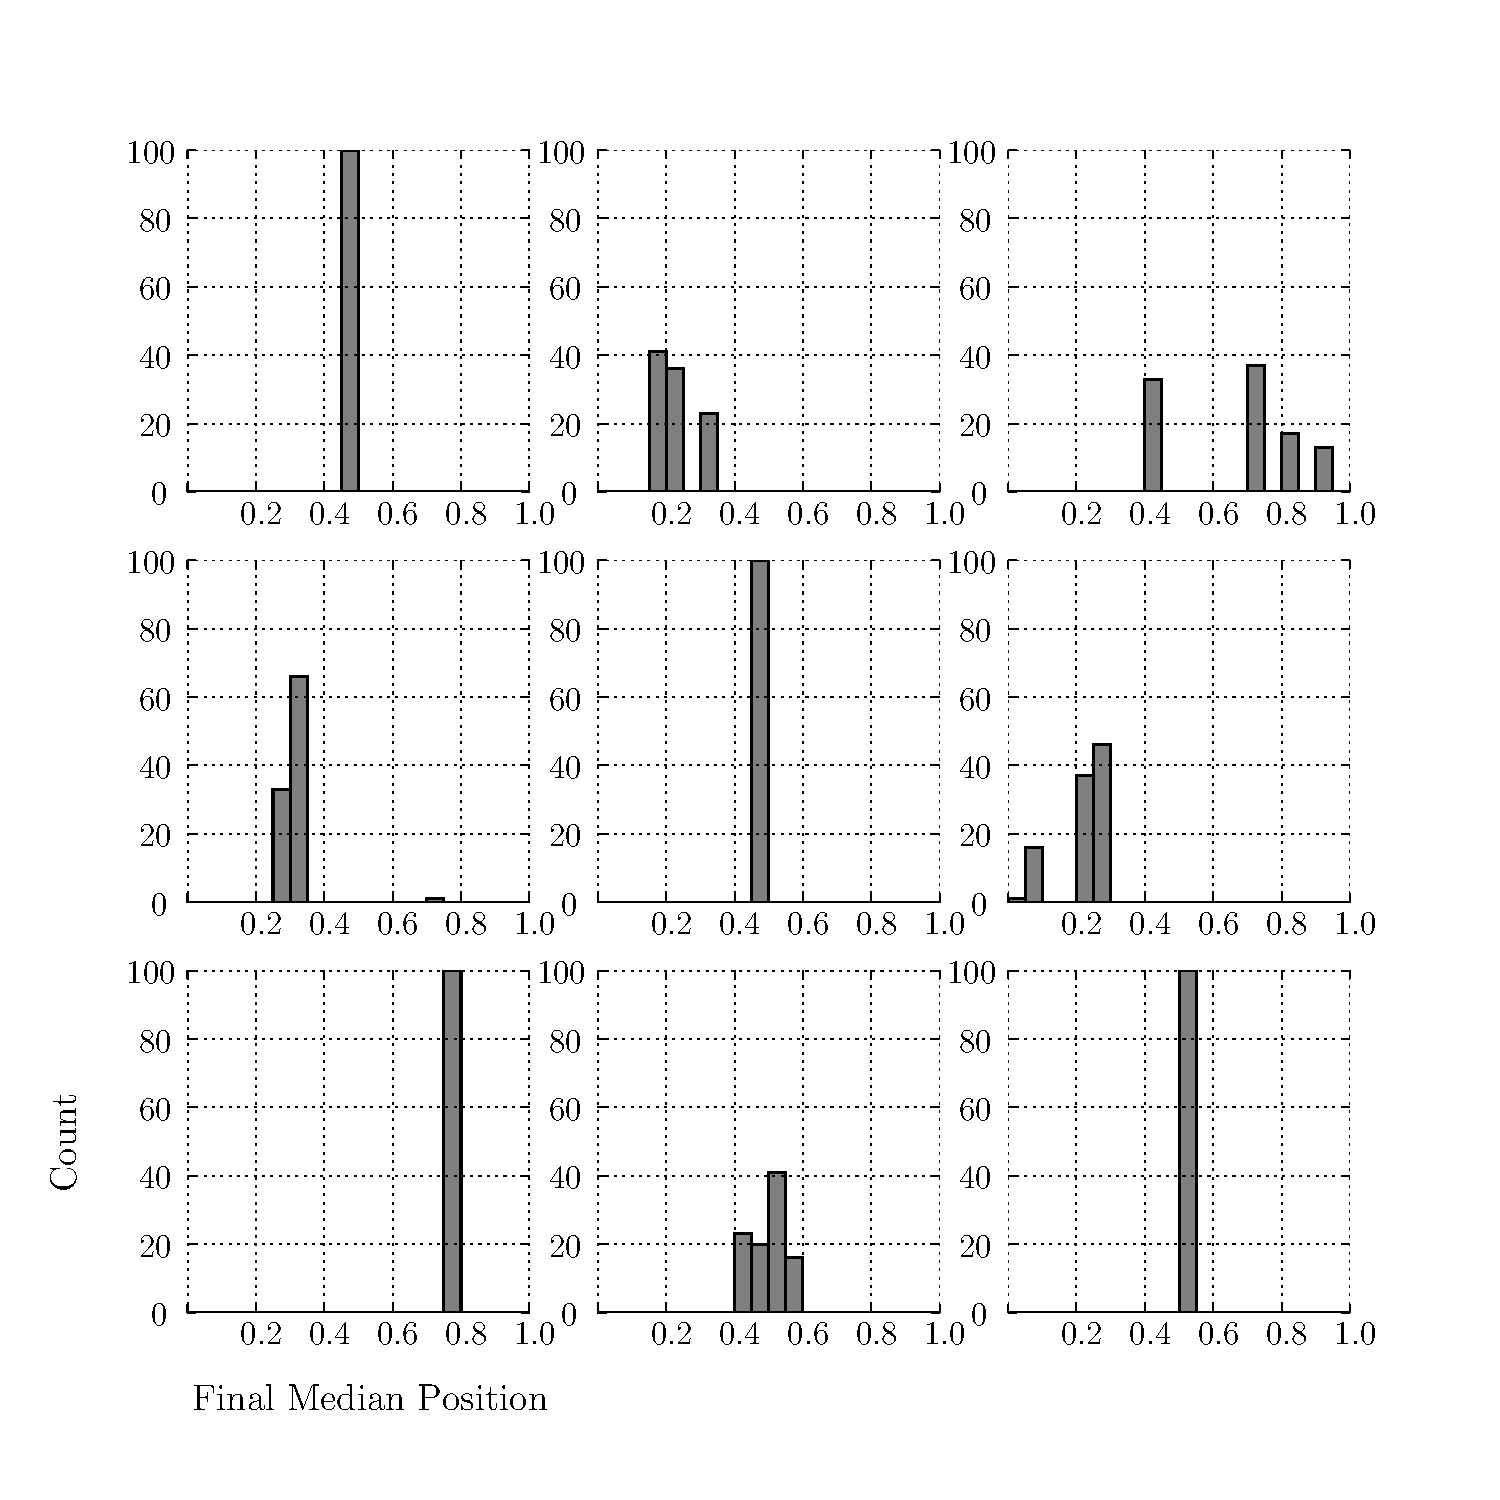
\includegraphics[width=\textwidth]{BDM_Reproduction/Figures/RandomGamesHist1}
        \caption{Experiment 1}
    \end{subfigure}
    \begin{subfigure}{0.49\textwidth}
        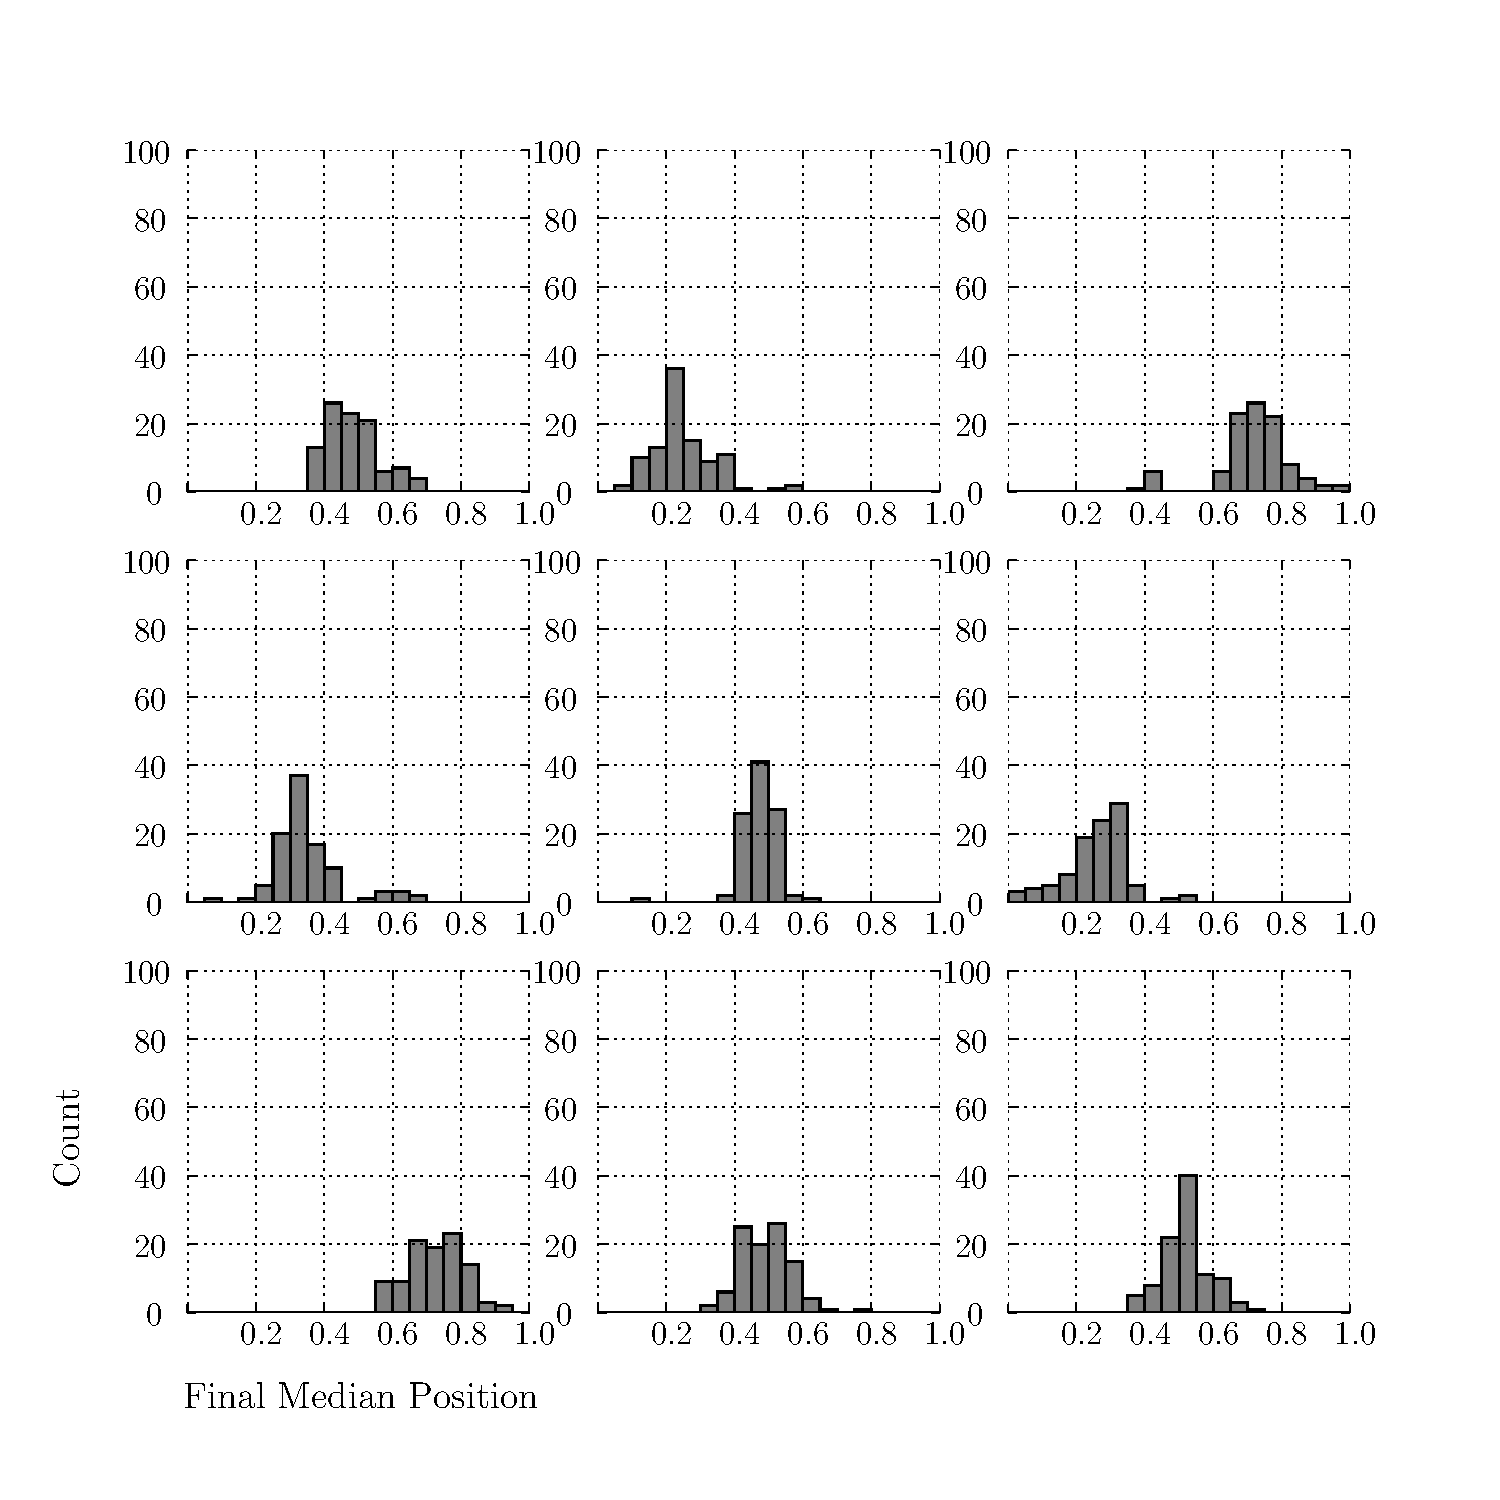
\includegraphics[width=\textwidth]{BDM_Reproduction/Figures/RandomGamesHist2}
        \caption{Experiment 2}
    \end{subfigure}

    \caption[Histograms of Median Positions]{Histograms of Median Positions from Nine Artificial Cases}
    \label{fig:random_medians}
    \figSpace
\end{figure}

Next, we can attempt to characterize the resulting distributions. Visual examination suggests that many of the resulting distributions are approximately normal. Applying the \citet{dagostino_1971} normality test to each dataset shows that only 25 of the cases generate normal distributions of outcomes in Experiment 1, while 43 do so in Experiment 2.

\begin{figure}
    \centering
    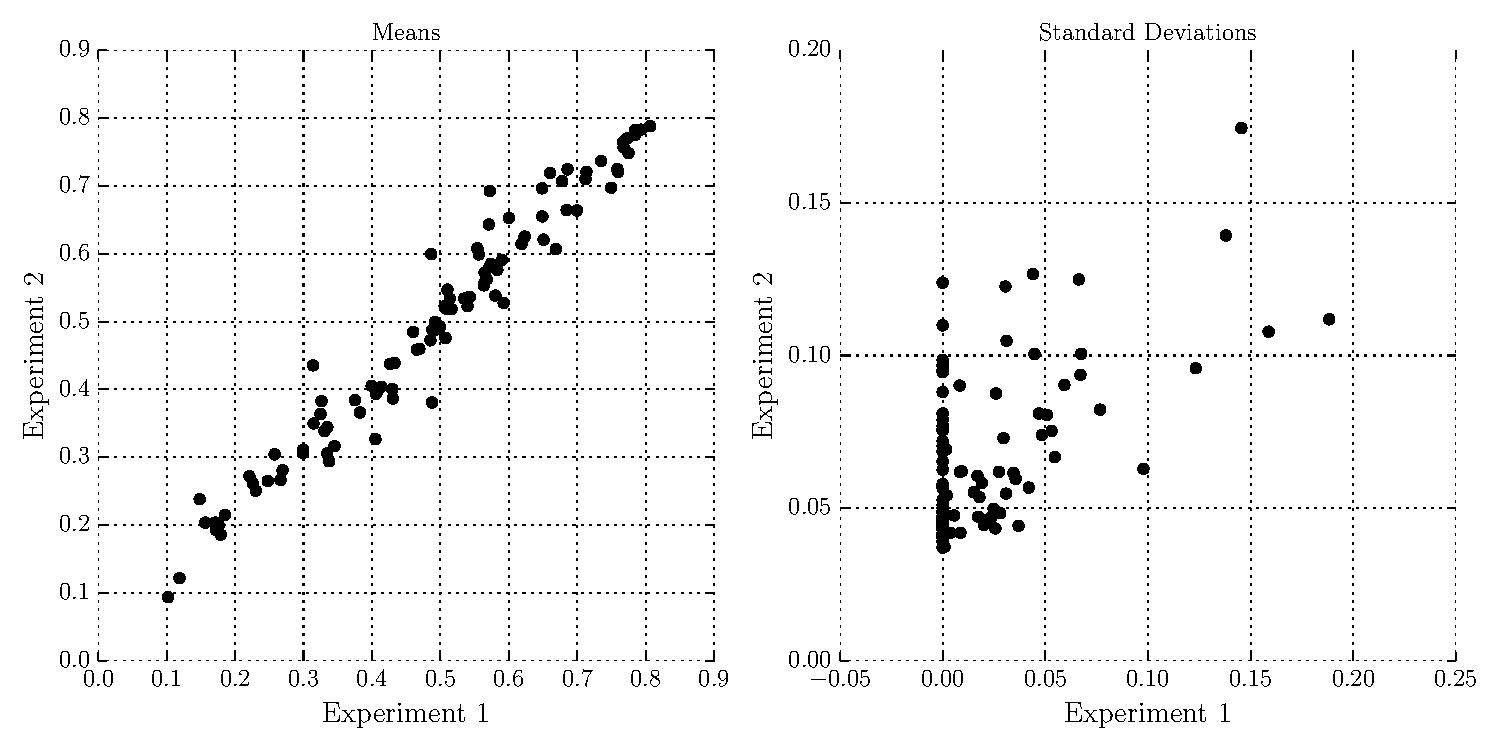
\includegraphics[width=\textwidth]{BDM_Reproduction/Figures/RandomGamesComparison}

    \caption{Experiment 1 and 2 Comparison}
    \label{fig:random_comparison}
    \figSpace
\end{figure}

Figure \ref{fig:random_comparison} compares the mean and standard deviation of outcomes from each case across both experiments. The key thing to observe is that the means of both are nearly identical. This means that though the perturbations of Experiment 2 increase the range of possible outcomes, they remain centered on the same outcome value; at no point does the perturbation appear to drive the model to a distribution qualitatively different from the non-perturbed outcomes. Additionally, the perturbation generally -- though not always -- increase the uncertainty of the model outcome, as measured by the outcomes' standard deviation. Furthermore, cases with similar degrees of uncertainty without perturbation (including no uncertainty, in the case of convergent cases) can yield different degrees of uncertainty once perturbed. 


\section{Information Extraction} \label{info_extraction}

At its most basic level, this model is meant to predict the outcome of the issue under negotiation. The outcome is generally defined as the median voter positions \citep{black_1948}: the position currently held by one of the actors which would defeat all other positions in bilateral contests. However, this may not be the most useful piece of information the model provides, particularly since many issues do not end up being resolved by a `vote,' or indeed resolved at all. In this section I will describe several additional outputs which can be extracted from the model, analyzed in their own right, and compared to empirical data.

One key piece of information the model generates is the set of the positions held by each actor at each iteration, and the trajectories of these positions. In cases where the position values represent concrete outcomes, the model provides a prediction (either a point prediction or a distribution) of the position each specific actor will hold. By examining how each actor's position changes, we can estimate the firmness of their position within the broader system being modeled. 

Furthermore, actor positions represent not just particular desired outcomes, but alignment with regard to other actors in a particular model run. If the model predicts two or more actors' positions moving together, we can interpret this as a prediction of cooperation, and potentially a formal or informal alliance, between these actors. Certainly, it is a prediction of convergent interests. This interpretation is shown in \citet{bdm_1998}, where certain model runs have agents' positions converging in ways that qualitatively resemble real-world alliances. This methodology can be formalized, by using the simulated distances between agent positions as a predictor for alliances or other relationships between the corresponding states. These distances can be used as an independent variable in several models, with alliances as the dependent variables: most simply a logistic regression, or network methods such as exponential random graph models (ERGMs) \citep{robins_2007} or latent space models \citep{hoff_2002}.

The model does not just generate positional predictions; each step generates discrete events from each interaction between a dyad of actors. While there is not have a clear mapping between model steps and real-world time, model-generated events can be compared to historic events within a window of interest; alternatively, the sequence of events can be compared, without taking into account the time-difference between them. Across multiple model instantiations, we can examine the frequency at which different events occur, either across an entire run or within a specified number of steps. 

The most obvious events, of course, are conflicts. Every model run may generate sets of conflict events when one or both of a pair of agents (depending on the model variant) choose to engage in conflict with each other. Conflict events are the most well-documented type of event in international relations, recorded in multiple specialized datasets \citep[e.g.][]{jones_1996,leng_1988,hendrix_2013} and are over-represented in media-coded event datasets \citep{schrodt_2001b}. This is particularly true when the conflict is overt between major political actors: military action is more likely to be recorded, while verbal conflict inside of a closed negotiation session less so.

Each conflict also creates a set of secondary events, with regard to the actors contributing capability to one side or another. The model does not specify what form this contribution takes; in reality, corresponding events may be positive actions towards the actor being supported (e.g. transfers of weapons or other materiel, favorable economic considerations), or negative actions towards the other side of the conflict (e.g. sanctions, withdrawal of support or access to resources). There may even be cooperative events observed between actors who are both supporting the same third party in its own conflict.

Offers are also events, though their correspondence with real events is also difficult to interpret. The model generates a much larger number of offers than end up being chosen, or even having a direct effect on the decisionmaking of the receivers. However, inasmuch as a conflict can only happen in the presence of threats, these threats may be treated as low-intensity conflict events as well.

\section{Comparing Model to Event Data} \label{icews}

The section above described how the model generates dyadic events, which can be compared to observed data. In this section, I describe implementing such an analysis in practice. I will walk through the instantiation of a set of geopolitical model runs using multiple different model variants, and comparing the conflicts they generate with observed micro-level event data in order to test and compare how well each explains the observed events. 

I set up several model variants, each using some different combinations of sub-models, based on different assumptions. I instantiate each with the same country-level agents with data from 2004, a year chosen arbitrarily for being well-covered by event data sets and lacking any major geopolitical shocks in the following years. I run each instantiation of the model for 24 steps, corresponding to approximately two years of `real' time. This mapping is somewhat arbitrary, but is based on the conventions which have developed for aggregating event data \citep{yonamine_2011}. In general, states do not change position or decide to begin or end confrontations with others on a day-by-day basis; however, neither do they do these things only once per year. Running these models multiple times produces a set of simulated events. I then run several tests to measure whether these simulated events are useful as predictors of real events. Comparing the predictive power of the model variants to one another can allow us to assess which variant is more predictive -- and thus, be provide evidence in support of their underlying assumptions.

\subsection{Data Sources} \label{data_sources}

\subsubsection{Event Data}

Real-world event data will serve as the dependent variable we are attempting to predict. The event data source I use for this is the Integrated Crisis Early Warning System, or ICEWS. This is a dataset of international political events, and specifically actions, extracted and machine-coded from media sources \citep{boschee_2015}. Each event consists of a Source (who carried out the action), a Target (who the action was directed at), and a code for the action itself. Actors (sources and targets) are coded to country, sector (e.g. government, civilians, rebels) and when possible to unique entities. Actions are assigned an Intensity score, where positive and negative values are associated with positive and negative actions, respectively. ICEWS has been assessed as being the most complete and reliable of several similar event datasets currently available \citep{ward_2013b}; however, on principle this analysis could be conducted with other event datasets as well.

In order to extract events which can be directly compared to model output, I subset the data and select events meeting the following criteria:

\begin{itemize}
    \item Occurring in the years 2005-2006, so that they are strictly following the input data.
    \item Where both the Source and Target actors are coded with the Government sector. This excludes events involving civilians, rebels, and other actors not explicitly captured in the model.
    \item Where the Source and Target countries are different, excluding internal events.
\end{itemize}

With these criteria, I aggregate the events into counts of event type by directed dyad. For the purposes of this analysis, I am not looking at the ordering of these events with respect to one another, but merely that they occur. 

\subsubsection{Input Data}

Following the methodology in \citet{bdm_1998}, I set agent properties based on the Correlates of War (COW) dataset: specifically, the alliance \citep{gibler_2004} and national material capabilities (NMC) \citep{singer_1988,grieg_2010} datasets. 

Using the material capabilities dataset, I select the 50 states with the highest Composite Index of National Capability scores. These are the model agents, and their CINC values are used as their capabilities. Since capabilities are always used in the model to compute ratios, there is no need to normalize these scores any further. Salience values will be set randomly, as described below.

Next, I use the COW alliance data to estimate positions. Taking advantage of the so-called unipolarity of the international system \citep{wohlforth_1999}, I will set each actor's initial position as the similarity of its alliance portfolio to that of the United States. Similarity of alliance portfolio has been used an approximation of the alignment of two countries' interests \citep{bdm_1975}, and alignment with the system's most powerful actor serves as a rough estimate of geopolitical position. 

Using  the alliances in effect in the selected instantiation year of 2004, I assemble an undirected network of state-to-state relationships, with the relationship coding as the weight\footnote{Note that this network includes all the actors present in the COW data, not just the top 50 actors who will be included in the model: as we are using the network to estimate similarity of positions, even countries which are not powerful enough to be worth including as agents can serve as indicators of countries' interests, and thus worthwhile to include in the network}. Using the resulting network's adjacency matrix, I compute the tau-b similarity \citep{bdm_1975} between country rows, and specifically between each country's row and that of the United States.

%
%\begin{figure}
%  \centering
%  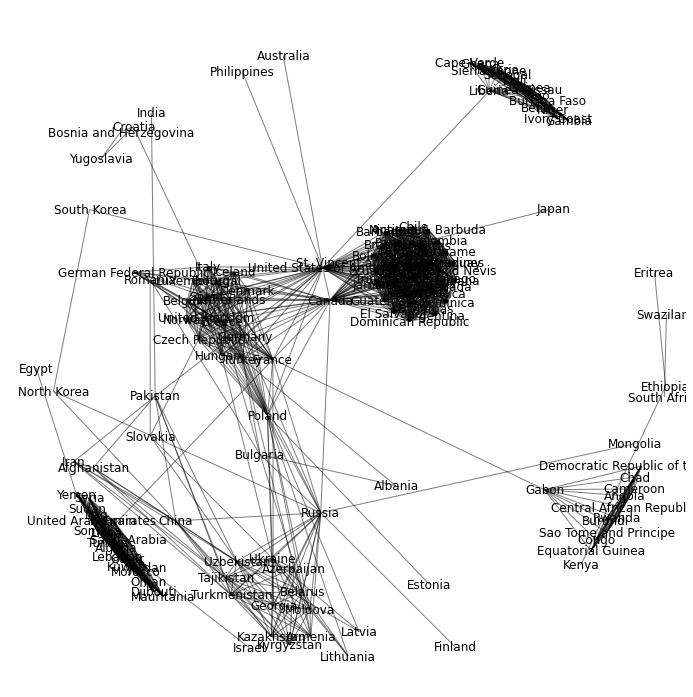
\includegraphics[scale=0.5]{BDM_Reproduction/Figures/Alliances2004}
%  \caption{Alliance network in 2004}
%  \label{fig:alliances_2004}
%  \figSpace
%\end{figure}
%
%\subsection{Model Setup}

Using the NMC and estimated positional data, I instantiate a model with 50 agents, one per state. There are 8 states which do not appear in the alliance network; at the beginning of each instantiation, I arbitrarily assign each a position of 0.5 + $\epsilon$, where $\epsilon \sim Normal(0, 0.1)$. The random perturbation is in order to prevent them from becoming a single alliance bloc. 

\begin{table}[h!]
\centering
\caption{Model Parameters}
\label{table:model_parameters}
\begin{tabular}{cl}
    \hline
    Variable &  Value \\
    \hline
    $s_i$            &        $\sim Unif(0, 1)$          \\
    $Q_i$            &   $0.5$ \\
    $T_i$            &   $0.5$ \\
    \hline
    Number of steps per run &        $24$ \\
    Number of instantiations &        $100$ \\
    \hline
\end{tabular}
\tableSpace
\end{table}

Unlike position and capability, there is no dataset giving us a-priori information on the agents' salience, particularly when the issue is relatively broad, as it is here. Thus, I apply salience updating rule $\mathbf{S_2}$: for each model instantiation, I set all the agents' saliences randomly, such that $s_i \sim Unif(0,1)$. As it is unlikely that shocks changing agents' salience will occur on a monthly basis, I hold these saliences constant throughout all 24 steps; this simplifying assumption removes one source of noise. This also corresponds to the assumption in \citet{bdm_1998} (which is also used in the following chapter), whereby agents' saliences are re-randomized on timesteps corresponding to approximately two years.


\begin{landscape}
\begin{table}
\centering
    \caption{Agent Data}
    \label{table:icews_agent_data}
\begin{tabular}{lcc|lcc}
    \hline
        Name                             & Position & Capability & Name                     & Position & Capability \\
    Algeria                          & 0.007    & 0.005      & Mexico                   & 0.734    & 0.012      \\
    Argentina                        & 0.732    & 0.005      & Morocco                  & 0.007    & 0.004      \\
    Australia                        & 0.192    & 0.007      & Myanmar                  & --      & 0.007      \\
    Bangladesh                       & --       & 0.008      & Netherlands              & 0.548    & 0.006      \\
    Belgium                          & 0.548    & 0.005      & Nigeria                  & 0.059    & 0.007      \\
    Brazil                           & 0.734    & 0.024      & North Korea              & 0.229    & 0.013      \\
    Canada                           & 0.907    & 0.011      & Pakistan                 & 0.092    & 0.013      \\
    Chile                            & 0.732    & 0.003      & Philippines              & 0.192    & 0.006      \\
    China                            & 0.115    & 0.183      & Poland                   & 0.45     & 0.007      \\
    Colombia                         & 0.734    & 0.006      & Romania                  & 0.271    & 0.004      \\
    Democratic Republic of the Congo & 0.072    & 0.004      & Russia                   & 0.141    & 0.045      \\
    Egypt                            & 0.192    & 0.009      & Saudi Arabia             & 0.007    & 0.009      \\
    Ethiopia                         & 0.17     & 0.004      & South Africa             & 0.192    & 0.007      \\
    France                           & 0.485    & 0.02       & South Korea              & 0.17     & 0.024      \\
    Germany                          & 0.55     & 0.027      & Spain                    & 0.548    & 0.011      \\
    Greece                           & 0.514    & 0.004      & Sweden                   & --       & 0.005      \\
    India                            & 0.324    & 0.07       & Syria                    & 0.008    & 0.004      \\
    Indonesia                        & --       & 0.013      & Taiwan                   & --       & 0.008      \\
    Iran                             & 0.168    & 0.012      & Thailand                 & --       & 0.008      \\
    Iraq                             & 0.007    & 0.006      & Turkey                   & 0.475    & 0.014      \\
    Israel                           & 0.192    & 0.004      & Ukraine                  & 0.088    & 0.014      \\
    Italy                            & 0.548    & 0.019      & United Kingdom           & 0.548    & 0.021      \\
    Japan                            & 0.192    & 0.047      & United States of America & 1        & 0.143      \\
    Kazakhstan                       & 0.056    & 0.003      & Venezuela                & 0.734    & 0.005      \\
    Malaysia                         & --      & 0.004      & Vietnam                  & --      & 0.008     \\
    
    \hline
\end{tabular}
\tableSpace
\end{table}

\end{landscape}


\subsection{Model Variants}

There are multiple possible permutations of the various sub-model variants presented in Sections \ref{model_description}. In this section, I will test a subset of them, attempting to cover a range of possible differences. In light of the coercion question I discuss in \ref{conflict_coercion}, I vary the conflict sub-models $\mathbf{W_0}$ and $\mathbf{W_1}$ across several variants. Recall that $\mathbf{W_0}$ has the loser in each conflict adopt the winner's position, while in $\mathbf{W_1}$ conflicts lead neither actor to change position.

\begin{description}
    \item[Model 1a]: This is the attempted replication of the original BDM model, as described in detail in Section \ref{model_description}. It comprises the sub-models  $\{\mathbf{T_0, S_2, W_0, R_0, O_0, M_0, A_0}\}$
    \item[Model 1b]: This model variant is identical to the one above except for the conflict sub-model. This variant will test the hypothesis that removing explicit coercion would make the model better reflect reality, and hence improve its explanatory and predictive power. $\{\mathbf{T_0, S_2, W_1, R_0, O_0, M_0, A_0}\}$
    \item[Model 2a]: This model implements several of the model variants together, while adhering to the overall structure of the original. Importantly, it implements the modified conflict schedule, with conflicts occurring only after agents have changed position in response to offers. $\{\mathbf{T_1, S_2, W_0, R_1, O_0, M_1, A_0}\}$
    \item[Model 2b]: Similarly, this model implements the previously-discussed variants, changing the conflict model. $\{\mathbf{T_1, S_2, W_1, R_1, O_0, M_1, A_0}\}$
    \item[Model 3a]: This model variant is the most different from the baseline. In addition to the new schedule and risk sub-models, it implements the balancing and attack follow-through sub-models. Unlike the other model variants here which require both agents in a conflict to choose to enter into it, this variant allows for unilateral attacks. $\{\mathbf{T_1, S_2, W_0, R_1, O_0, M_2, A_1}\}$
    \item[Model 3b]: Finally, once again, this variant is identical to the previous one, but uses the alternative conflict sub-model. $\{\mathbf{T_1, S_2, W_1, R_1, O_0, M_2, A_1}\}$
\end{description}

\subsection{Experiments and Results}

For each model variant, I instantiate 100 model runs with the data in Table \ref{table:icews_agent_data}. I then run each for 24 steps. For each model run, I extract the Conflict events that the model generates. I aggregate these events across all runs for each dyad, and compute the mean conflict events for each dyad. These mean conflicts are the independent variables. 

\begin{figure}[t!]
    \centering
    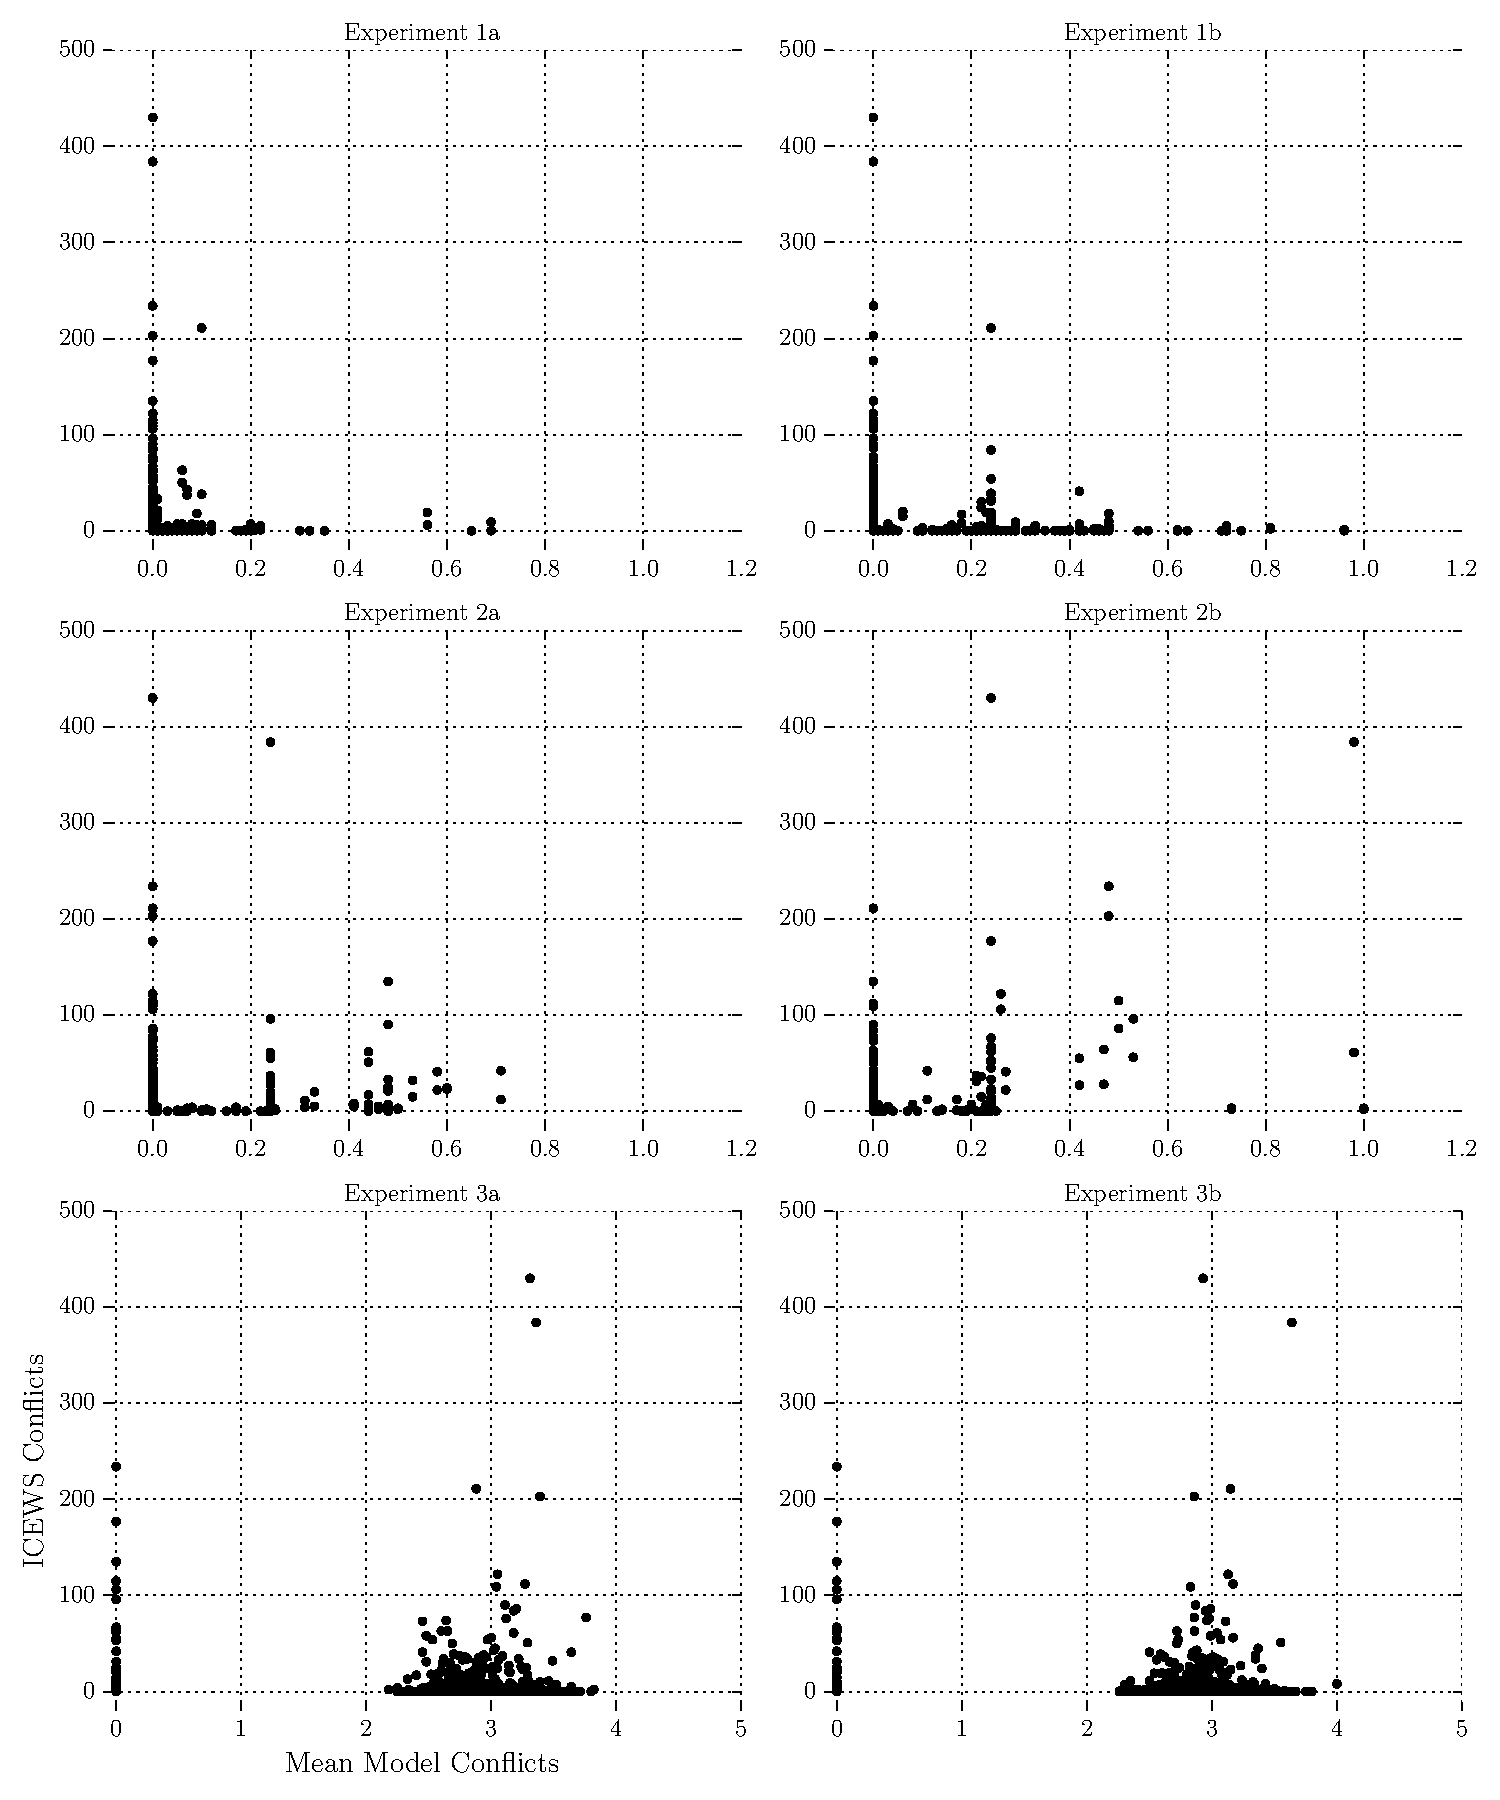
\includegraphics[width=\textwidth]{BDM_Reproduction/Figures/ICEWS_Scatters}
    \caption{Model-Generated vs ICEWS Conflict Events}
    \label{fig:icews_scatters}
    \figSpace
\end{figure}

The dependent variables are the conflict-coded events for each dyad drawn from the ICEWS dataset for the 2005-06 period, as described above in Section \ref{data_sources}. Figure \ref{fig:icews_scatters} shows the scatter-plots of total model-generated conflicts versus ICEWS conflict events for each dyad. It is immediately obvious that a large portion of these two result sets are orthogonal: many dyads with ICEWS conflicts do not have model conflicts, and vice versa.  I next test whether, for each model variant, the simulated events it generates have any predictive power for the volume of conflict events predicted for each dyad. I conduct two sets of regressions, on two variables: a linear model on the number of observed conflict events (Table \ref{table:icews_linear}), and a logistic regression on whether any conflicts were observed across each dyad (Table \ref{table:icews_logit}). In both cases, the mean model-generated conflicts are be the independent variable. 

These are relatively simple statistical models; in particular, we have no reason to expect there to be a linear relationship between simulated and observed conflicts. However, these regressions will allow us to identify whether a relationship exists at all between the simulated and observed events, and what direction that relationship is -- in general, we expect that if a model is generating plausible conflicts, there will be a positive relationship between simulated and observed conflict events. Furthermore, since the dependent data is the same across all model variants, we can directly compare the coefficients and fit to determine which model is closer to reality.


\begin{table}

\begin{center}
    \caption{ICEWS Conflict Events -- Linear Regressions}
    \label{table:icews_linear}
\begin{tabular}{lcccccc}
    \hline
                    &    1a   &    1b    &    2a    &    2b    &    3a    &    3b     \\
    \hline

    Const.          & 2.82*** & 3.91***  & 2.27***  & 1.40***  & 20.37*** & 21.80***  \\
                    & (0.35)  & (0.44)   & (0.35)   & (0.33)   & (2.10)   & (2.10)    \\
    Mean Model Conflicts & 6.82    & -7.90*** & 33.58*** & 94.31*** & -6.20*** & -6.64***  \\
                    & (8.61)  & (1.99)   & (4.57)   & (4.38)   & (0.73)   & (0.73)    \\
    \hline
    $R^2$             & 0.00    & 0.01     & 0.02     & 0.16     & 0.03     & 0.03      \\
    \hline
    \hline
    \multicolumn{7}{l}{Standard errors in parentheses.} \\
    \multicolumn{7}{l}{* $p<.1$, ** $p<.05$, *** $p<.01$} \\

    \end{tabular}
    \end{center}
    \tableSpace
\end{table}

\begin{table}
\begin{center}
    \caption{ICEWS Conflict Events -- Logistic Regressions}
    \label{table:icews_logit}
\begin{tabular}{lcccccc}
    \hline
                    &    1a   &    1b    &    2a    &    2b    &    3a    &    3b     \\
    \hline
    Const.          & -1.19*** & -1.03*** & -1.30*** & -1.32*** & 1.22***  & 1.47***   \\
                    & (0.05)   & (0.06)   & (0.05)   & (0.05)   & (0.30)   & (0.31)    \\
    Mean Model Conflicts & 2.27**   & -1.15*** & 5.52***  & 8.01***  & -0.86*** & -0.94***  \\
                    & (1.03)   & (0.30)   & (0.62)   & (0.81)   & (0.10)   & (0.11)    \\
    \hline
    Pseudo $R^2$      & 0.00     & 0.01     & 0.03     & 0.05     & 0.03     & 0.04      \\
    \hline
    \hline
    \multicolumn{7}{l}{Standard errors in parentheses.} \\
    \multicolumn{7}{l}{* $p<.1$, ** $p<.05$, *** $p<.01$} \\
    \end{tabular}
    \end{center}
\tableSpace
\end{table}

Examining Table \ref{table:icews_linear} immediately shows us that there are substantial differences between the predictive power of the different models. The output of Model 1a, the original model, seems to bear no measurable relationship to the observed events. Models 1b, 3a and 3b have negative mean conflict coefficients, indicating that the more simulated conflicts we observe, the fewer real conflicts we can expect to see -- the opposite of the relationship we were hoping for. Only Models 2a and 2b have coefficients which are significant and positive, showing that the more conflicts these models predict, the more we can expect to see. Between these two, Model 2b has a substantially higher $R^2$ value, indicating a better fit. 

The same pattern holds when examining Table \ref{table:icews_logit}, which coarse-grains the ICEWS data further, asking whether more simulated conflicts make it more likely that we will observe any conflicts at all between the corresponding dyad. The coefficients show the same pattern of signs, indicating that only Models 2a and 2b generate simulated conflicts which are useful for predicting real conflicts. Between these, again, Model 2b shows a better fit, though the advantage is less stark here.

%In order to further test whether these models are providing useful new information, I repeat the regressions above, with an additional variable: the tau score for each dyad, or the estimated similarity of the two actors' interests to one another. Based on theory, we would expect more observed conflict events between actors with lower tau scores. The results of these regressions are shown in TKTKT. Two results jump out: first is that the coefficients on tau are positive, indicating more conflict events the more similar two actors are -- a surprising deviation from theory worth exploring in more detail, but outside the scope of this paper. More importantly, for our purposes, the \textbf{Model Conflicts} coefficients both remain small but positive, with only the baseline variant remaining statistically significant. This indicates that the baseline model, at least, is indeed generating new information rather than simply arriving at the same result as the tau-based analysis via a circuitous route. 

\subsection{Discussion}

With these results in hand, we can draw several conclusions. At the crudest level, we see that across all the model variants, the number of conflict events generated is much smaller than the number of observed conflict events. Many dyads with recorded conflict events are not predicted by the models, while the models in turn predict conflicts across many dyads where none are observed. The overall relationships between the model outputs and observed data are weak.

Despite this, we must recall that there are countless issues that at any given time are driving the micro-level interactions between countries in the world. Across all the model variants presented here, we have attempted to capture only those issues reflected in states' alliances, and further compressed them onto a single one-dimensional space. Given the simplicity of the model itself, and the global scope that these particular instantiations are addressing, and it appears remarkable that there is any statistical relationship between the model output and reality at all. And indeed, several of the model variants -- particularly 2a and 2b -- appear to be valid predictors of real-world conflicts, at least as captured by the ICEWS data.

Furthermore, this methodology allows direct comparison between model variants, each comprising combinations of different sub-models. Examination of the scatter-plots of Figure \ref{fig:icews_scatters} shows us that different variants generate different patterns of events. We can immediately see, in particular, that Models 3a and 3b generate a higher volume of conflict events, and that the quantities for each dyad are approximately normally-distributed, conditional on there being any conflicts at all for those dyads. We can also immediately identify that variants 2a and 2b outperform the other variants as predictors, and that between the two of them variant 2b has superior predictive power. This, in turn, is in line with my hypothesis that the conflict sub-model $\mathbf{W_1}$, where conflicts do not result in agents changing their position, is more correct than the baseline variant $\mathbf{W_0}$.

\section{Conclusions}

In this chapter, I have argued that Bruce Bueno de Mesquita's Expected Utility Model is best understood not as a game-theoretic model but as an agent-based one. The model and its agents are composed of several sub-models, with the agents interacting with one another following certain behavior rules. These rules, in turn, are based on heuristics and embedded assumptions that are not addressed in prior papers describing the model and its applications. I have described my reimplementation of the model as an object-oriented agent-based model. While doing so, I was able to identify its sub-models and heuristics, and discuss how they fit together -- and how they may be altered and experimented with.

My reimplementation of the model was unable to reproduce several results generated by the original model and reported in the prior literature, in particular the results of \citet{bdm_1994} and \citet[chapter 6]{bdm_2002}. It is possible that despite my best efforts, my own model code misimplements one of the formulas from the prior literature, or has another unintentional uncaught bug which is the cause of the difference between its outputs and the prior results. It is also possible that I have implemented one of the sub-models which is not well described in the prior literature (particularly the offer acceptance sub-model) differently from the original model. Without access to the original application or source code, it is impossible to fully isolate the source of the differences. Nevertheless, I do have access to the source code of the \citet{scholz_2011} model implementation, as well as to a replication of that implementation \citep{mckibben_sanders_2014}, both of which successfully reproduce the \citet{bdm_1994} results. As I discuss in Section \ref{verification}, I identify a key way in which this implementation contradicts both the stated form and underlying assumptions of the original model, by having the probabilities of victory in a bilateral conflict not sum to 1. It may be the case that by coincidence this model implementation featured multiple errors which lined up to produce the right results for the wrong reasons; however, as \citet{scholz_2011} themselves note, the odds of generating correct results by chance are extremely low. It seems more likely that they have inadvertently identified an error in a particular implementation of the original model -- one which, presumably, was corrected in later versions. Importantly, the \citet{scholz_2011} implementation was unable to replicate results reported in other publications. This tells us that their implementation cannot be considered a perfect replication either -- and that published original model results cannot necessarily be treated as `ground truth' either.

In Section \ref{sensitivity-analysis}, I described and implement a sensitivity analysis methodology using randomly generated cases. This analysis indicates that the original model has little meaningful stochasticity, and that in some cases converges to a single median outcome. In fact, it suggests that there are two distinct classes of input sets, ones which have deterministic outcomes and ones that do not. This distinction should be investigated further, in particular in applications of the model to the analysis of real-world cases. Even relatively slight perturbation of the model inputs introduced an additional source of stochasticity, eliminating the determinism. It also does not appear to be the case that convergent models have less uncertainty once the inputs are perturbed, suggesting that the convergence is an artifact of the specific input parameters rather than evidence that the system itself has an inherent attractor. However, the means of the perturbed runs tend to remain very close to the unperturbed mean; the perturbation doesn't push the system into a meaningfully different region of the outcome range. This finding, in turn, lends justification to practice of original model results being reported as point predictions rather than distributions.

The model itself is driven largely by heuristics, with the model and agent behavior not always grounded in specific theories or sources. This on its own is not necessarily a major flaw, and indeed is common for other agent-based models of international relations \citep[e.g.][]{axelrod_1997,taylor_2008}. By reimplementing the model as an ABM, I was able to highlight these heuristics and assumptions to a greater extent than had been previously reported. More importantly, this implementation makes it straightforward to test the model with different sub-models and heuristics reflecting different assumptions. I have proposed several such variant sub-models, as well as a notation system to quickly describe different model variants comprising different sub-models.

By enabling multiple model variants to be run with the same input data, I also test the predictive power of those variants side by side. Political event data provides a source of relevant real-world interactions, and to the best of my knowledge, no EUM-type model has been applied to event data before. However, as I argue in Section \ref{info_extraction}, the dynamics and outputs of the model correspond naturally to categories present in event data. Indeed, I demonstrate in Section \ref{icews} that even using a coarse instantiation without a well-defined issue of contention, several variants of the model generate sets of simulated events bearing weak but statistically significant predictive power for corresponding real-world events. 

More important than the specific findings of these models, however, is a demonstration of how such models can be applied comparatively. By using fixed input data and the same target output data, we can run multiple instantiations of different model variants, generating sets of model traces -- and especially sets of simulated conflict events -- for each. This allows us to find the different patterns which emerge from different models, such as the difference in conflict distributions between model variants 1, 2 and 3 visible in Figure \ref{fig:icews_scatters}. By regressing the model outputs against observed data, we can test which among several models has more explanatory or predictive power. Comparing the performance of model variants which differ only by a single sub-model (such as 3a and 3b above, which implement conflict rules $\mathbf{W_0}$ and $\mathbf{W_1}$, respectively) can highlight the effects of those sub-model variants, and allow us to test the hypotheses they describe.

The model and methodology I have described here mark the beginning, not the end, of a program of study. I have explored only a subset of possible combinations of the sub-models I have presented here, which in turn are only a subset of plausible sub-model variants. Applying the sensitivity analysis to additional model variants will allow us to characterize inherent dynamics or artifacts that the variants exhibit, which in turn can help isolate meaningful predictions when instantiated with real data. Testing these models against different cases and sets of political actors will help identify whether one mode variant is strictly superior, or whether different variants are appropriate for different categories of cases and issues. It may also be the case that ensembles of model variants may provide greater predictive power than any single variant alone. 

There are still assumptions embedded in the current architecture, independent of any sub-model. For example, conflicts are currently strictly bilateral, and agents contributing capability to one side or another face no effects if the principals win or lose, unlike in the \citet{wise_2015a} model framework. Similarly, the model as presented here only models issues as one-dimensional ranges; however, \citet{wise_2015b} have proposed an extension allowing their model to handle multiple issues, including ones represented non-numerically. The agent activation regime plays an important role in the behavior of agent-based models \citep{comer_2014}, and the validity of the simultaneous activation assumption may depend on the specifics of the scenario being simulated. The simultaneous activation the model currently features may be appropriate for modeling negotiators in close proximity (perhaps in the proverbial smoke-filled room) or when the actors are states acting over months or years, but may be less so for intermediate scales. Varying and sequencing agent activation may allow the model to incorporate time more explicitly, improve modeling of interactions between agents with different paces of decisionmaking, and endogenize incomplete information. 

There are likely other methods of utilizing models within the framework described here. I have conducted preliminary experiments with applying the model deductively: given observed sequences of events, to identify initial inputs which are most likely to give rise to similar sequences. This may allow us to estimate the actors' underlying preferences and capabilities in the absence of reliable quantitative data or even subject-matter expertise. My initial experiments suggest that such an application is computationally plausible, but that multiple, substantially different inputs may yield similar event sequences.

Finally, the findings I have described here provide reasons for both appreciation and skepticism of the original BDM model. Building on the published descriptions of the model have allowed me to build a generalized, flexible agent-based model of political interaction with rich outputs and surprising predictive power despite its relative simplicity. The sensitivity analyses I have conducted lend some credence to the practice of reporting the model's point results, though also highlight the degree to which this elides uncertainty that is indeed present in the model. The difficulty in reproducing the model from published descriptions should give us pause. I have identified numerous assumptions and heuristics in the model description, very few of which are explicitly stated, much less supported either theoretically or empirically. This makes it all the more important to implement not just a single model but multiple variants, in order to rigorously test and evaluate them. If we do so, however, it promises to offer a valuable tool for operationalizing and testing competing heuristics, intuitions and theories of competing political actors in the international system and beyond.


\chapter[Modeling the Cold War]{Modeling the Cold War: An Application of the Expected Utility Model}

\section{Introduction}

% 3. I suggest the tense of the discussion needs to be watched more closely.  Most things are past tense, but… on the first page, the quoting of T.S. Eliot should be past tense. and in 2.2.1, the 1998 paper doesn’t "generates the model inputs”, but "generated” them last century.

The Cold War between the United States and the Soviet Union (also refered to interchangeably as the Union of Soviet Socialist Republics, or USSR) was the defining feature of the international order in the second half of the 20th century, helping drive everything from local insurgencies to space exploration. The conflict was rooted both in ideological differences and a desire for security. Indeed, both sides possessed not only powerful conventional militaries with global reach, but arsenals of nuclear weapons capable of guaranteeing so-called Mutually Assured Destruction. Each side posed an existential risk not only to the other's system of government, but to the lives of a large proportion of their citizens. Both sides also had stable blocs of aligned countries; in Europe this divide was geographic, with the `Iron Curtain' separating the west and east. The apparent parity of the two sides, and the stability of their alliances, led to an expectation that the cold war between them would persist indefinitely, terminated perhaps only in apocalyptic conflict. 

Yet it was not the world but the Cold War, and the Soviet Union itself, which ended -- ``Not with a bang but with a whimper,'' as \citet{dobson_2007}, \citet{prados_2011} and others quote \citet{eliot_1934}. The end of the Cold War took policymakers and scholars both by surprise. In the aftermath, many political scientists \citep[e.g.][]{gaddis_1992,lebow_1995} suggested that this was evidence of shortcomings in the state of international relations theory and methodology. \citet{bdm_1998} offered an alternative explanation: that the end of the Cold War \emph{was} predictable by contemporary international relations theory, but that it was an emergent phenomenon: an unexpected higher-level outcome generated from the combination of multiple lower-level interactions which themselves are well-understood. Indeed, if the international system is complex, it should not be surprising for it to generate emergent phenomena.

\citet{bdm_1998} tests this claim by simulating the Cold War using the Expected Utility Model. Computational modeling is uniquely suited to generating macro-level emergent phenomena from micro-level interactions; thus, if the model is well-grounded in theory and gives rise to the end of the Cold War, this is evidence that the theory itself was not mistaken, but rather that it was not properly applied, or its implications not fully understood. Furthermore, if the model can outperform experts and predict a major historic outcome from the relatively minimal data it is instantiated with, this would be strong evidence in favor of the model's utility and predictive power. Indeed, this paper argued that such a model, and the EUM in particular, can predict the end of the Cold War, with a victory for the US and its allies.

In the previous chapter, I presented my own reproduction and extension of the Expected Utility model that \citet{bdm_1998} uses. In this chapter, I attempt to apply my model variants to the same Cold War case study. This serves several purposes. It attempts to replicate the previous study, while also providing an additional test of my reproduction: if my direct reimplementation model produces similar outcomes to the original, this is evidence for an accurate replication. Additionally, as with the original model, if my models are capable of successfully predicting the end of the Cold War from historic data, this is evidence of their usefulness. As discussed in the previous chapter, my own models extend the original by recording not just outcomes but key events that lead up to them. Comparing these events -- and in particular, conflicts -- to historic data provides an additional external test of the models' validity. Finally, by comparing the predictive power of different model variants, I can attempt to identify the one with the most explanatory power.

The rest of this chapter is organized as follows. I describe the input data (Section \ref{sec:input_data}), how I use it to instantiate runs of two model variants (Section \ref{models}), and data to which I will compare to model outputs (Section \ref{outputs}). In Section \ref{results}, I present the results of four experiments, each one a combination of an input dataset with a model variant. I describe the results of each experiment qualitatively, and test their output's power as a predictor of observed conflicts and post-Cold War alliances. Finally, In Section \ref{cw_discussion}, I discuss the results more broadly, highlighting and attempting to explain the models' strengths and weaknesses.

\section{Modeling Methodology}

The procedure for this analysis follows a similar process to that described in the previous chapter. Initially empirical data is used to generate a set of actors, with position and capability values for each. These actors then serve as inputs to the model variants, each of which is instantiated and run multiple times, generating collections of outputs. Finally, I analyze these outcomes and compare them to real-world data.

\subsection{Input Data} \label{sec:input_data}

To instantiate a model, we require several things: a list of agents, which in this case are countries active in the international system during the Cold War; and for each agent, an initial position on the one-dimensional position space and a capability value. There is no need here to attempt to estimate salience, since this will be one of the independent values which will be randomized for all agents, as described below.

\citet{bdm_1998} generated the model inputs from data collected by the Correlates of War (COW) project. The list of actors, and their capabilities, are drawn from the National Material Capabilities dataset \citep{singer_1972,singer_1988}, with the model using the 36 most-powerful actors in the starting year of 1948; their capabilities are normalized so that all capabilities sum to 100. Their positions are derived from the COW alliance dataset \citep{singer_1969}, measuring each agent's closeness to the security preferences of the United States or Soviet Union. This closeness is defined as the tau-b measure of similarity in alliance portfolios \citep{bdm_1975}, normalized such that a value of +100 is full match with the United States, and -100 is a full match with the Soviet Union. In order to make this data compatible with my implementation of the model, I simply rescale the starting positions so that they fall on the ${[0, 1]}$ range, with 0 being the Soviet Union's starting position and 1 being that of the United States. The original model inputs are reported in \citet{bdm_1998} and reproduced in Table \ref{table:bdm_inputs}, with the rescaled positions. I term this the Original Input data. Figure \ref{fig:original_input_hist} visually demonstrates the starting distribution of power: the United States and its core allies (those whose positions $\approx 1$) have a slight advantage in total capability over the Soviet Union and its core allies (position $\approx 0$); however, the largest capability bloc is in the center, not yet committed to either side.

\begin{table}
\centering
  \caption[Original Inputs]{Original Inputs \citep{bdm_1998} with Positions Rescaled}
  \label{table:bdm_inputs}
\begin{tabular}{lcc||lcc}
  \hline
  Country        & Capability & Position & Country      & Capability & Position \\
  \hline
  Argentina      & 0.972      & 0.948    & Italy        & 2.426      & 0.507    \\
  Australia      & 0.889      & 0.507    & Mexico       & 0.774      & 0.948    \\
  Belgium        & 1.182      & 0.514    & Norway       & 0.23       & 0.507    \\
  Brazil         & 0.993      & 0.948    & Netherlands  & 0.836      & 0.514    \\
  Bulgaria       & 0.345      & 0.000    & Pakistan     & 1.485      & 0.507    \\
  Canada         & 1.61       & 0.781    & Philippines  & 0.408      & 0.507    \\
  China          & 11.941     & 0.507    & Poland       & 3.273      & 0.045    \\
  Czechoslovakia & 1.401      & 0.045    & Romania      & 0.606      & 0.045    \\
  Denmark        & 0.24       & 0.507    & Saudi Arabia & 0.125      & 0.514    \\
  Egypt          & 0.408      & 0.516    & South Africa & 0.68       & 0.507    \\
  England        & 7.863      & 0.518    & USSR         & 18.256     & 0.000    \\
  France         & 3.597      & 0.514    & Spain        & 1.683      & 0.507    \\
  Greece         & 0.418      & 0.507    & Sweden       & 0.648      & 0.507    \\
  Hungary        & 0.45       & 0.045    & Syria        & 0.104      & 0.514    \\
  India          & 2.468      & 0.507    & Thailand     & 0.414      & 0.507    \\
  Iran           & 0.491      & 0.512    & Turkey       & 1.347      & 0.512    \\
  Iraq           & 0.157      & 0.519    & USA          & 29.956     & 1.000    \\
  Israel         & 0.125      & 0.507    & Yugoslavia   & 0.891      & 0.000    \\
  \hline
\end{tabular}
  \tableSpace
\end{table}

\begin{figure}
  \centering
  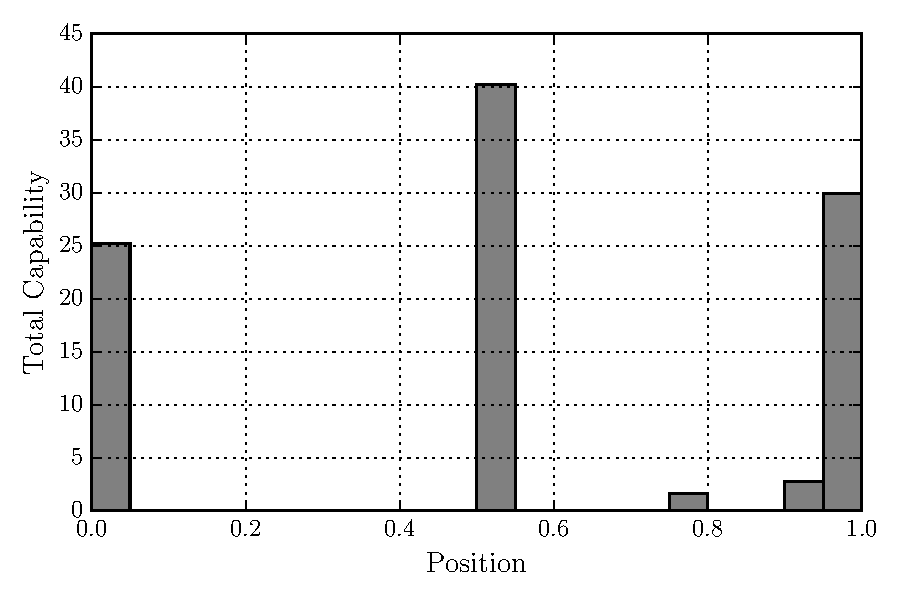
\includegraphics[scale=0.75]{ColdWar/Figures/Original_Inputs_hist}
  \caption[Original Inputs]{Original Inputs -- Initial Distribution of Capabilities}
  \label{fig:original_input_hist}
  \figSpace
 \end{figure}

%% [WGK]: 2. I’m concerned about what the numbers mean and with the lack of consistency in the use of significant figures in tables means for the content. Table 2.1, is mostly 3 significant figures. Ok, but they don’t seem to be when 13 of the 36 values for the position are the same, to 3 significant figures (0.507), yet there another 10 within 0.015. A histogram would be interesting and raise or dispel questions about the workings of the model. Related, Table 2.3, has numbers with apparently 2, 3, and 5 significant figures. How to they interact and what would the histogram tell us?


I then attempt to reproduce the input data from the current, up-to-date COW datasets \citep{gibler_2009,grieg_2010}; however, this did not result in the same inputs as provided in \citet{bdm_1998}. The initial difference is the capability scores -- not just the Composite Index of National Capability (CINC) scores themselves of the various countries for 1948, but their rankings as well. This is likely due to updated data and methodologies, but already indicates a difficulty in replicating the previous study. Since in this case I have access to all the countries for which there is 1948 data, I will include all of them in the model, rather than utilize an arbitrary cutoff.

Next, we must assign each agent to a position. To do so, I construct an undirected network from the most recent COW alliance data for 1948, where the edge between each pair of countries is coded based on the alliance type, as summarized in Table \ref{table:alliance_types}. We can then calculate similarity scores between the the actors' rows or columns in the adjacency matrix, which represent the actors' alliance portfolio. To maintain correspondence with the previous data, I use the tau-b similarity score between portfolios. 

\begin{table}[!h]
\centering
  \caption[Alliance Coding]{Alliance Coding \citep[descriptions quoted from][]{gibler_2013}}
  \label{table:alliance_types}
\begin{tabular}{p{2cm}p{6cm}}
\hline
Alliance Code & Type  \\
\hline
1             & Entente: ``one or both states in the dyad had an understanding that consultations with the other state in the dyad would take place if a crisis occurred.'' \\
2             & Non-Aggression: ``one or both states in the dyad had a non-aggression pact with the other state in the dyad.'' \\
3             & Neutrality: ``one or both states in the dyad had a neutrality pact with the other state in the dyad.'' \\
4             & Defense: ``one or both states in the dyad had a defense pact with the other state in the dyad.'' \\
\hline                                               
\end{tabular}
  \tableSpace
\end{table}

\begin{figure}[!h]
  \centering
  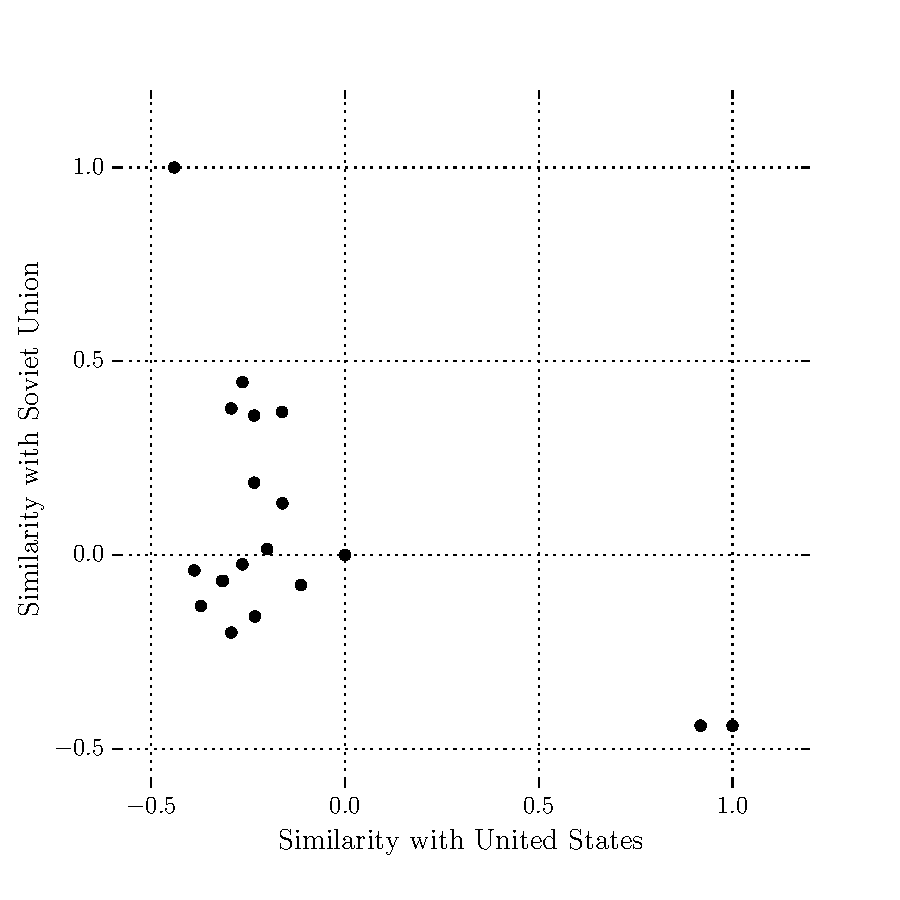
\includegraphics[scale=0.5]{ColdWar/Figures/us_sov_similarities}
  \caption{Tau-b Similarities of Actors to United States and Soviet Union}
  \label{fig:us_sov_corr}
  \figSpace
 \end{figure}

It is here that we run into a question unaddressed in \citet{bdm_1998}. Comparing each country's alliance portfolio to those of the United States and the Soviet Union produces not a single value per country, but two: one for each superpower. As shown in Figure \ref{fig:us_sov_corr}, the relationship between the similarities is not completely linear, meaning we need to choose a way to reduce the two-dimensional security position space to one dimension. Since the two dimensions are highly correlated (correlation coefficient $-0.81$), I use principal component analysis \citep{tipping_1999} to project the two-dimensional data onto a one-dimensional space, which I then rescale so that the values are between 0 and 1.

I term the new model inputs, appropriately enough, the Updated Input data; Table \ref{table:new_inputs} reports the new positions and capabilities\footnote{To make this data directly comparable with the original inputs in Table \ref{table:bdm_inputs}, I have rescaled the CINC scores so that they sum to 100. Since Capability scores are used solely as ratios, this rescaling has no effect on the model.}. This input set includes all the countries for which data is available in 1948. Like the original input data, it excludes Japan and West and East Germany, which had not yet become sovereign at that point. 
Figure \ref{fig:updated_input_hist} visually shows the initial distribution of power in this scenario: while in this case the United States and its core allies have an even larger advantage over the Soviet Union and its core allies than in the Original Input. The key difference, however, is that instead of a single bloc between the two powers' positions, there are agents at multiple intermediate positions; the single largest power bloc at approximately 0.6, dominated by China and India, is slightly closer to the United States, but there are more agents whose positions are closer to that of the Soviet Union.

\begin{figure}[h!]
  \centering
  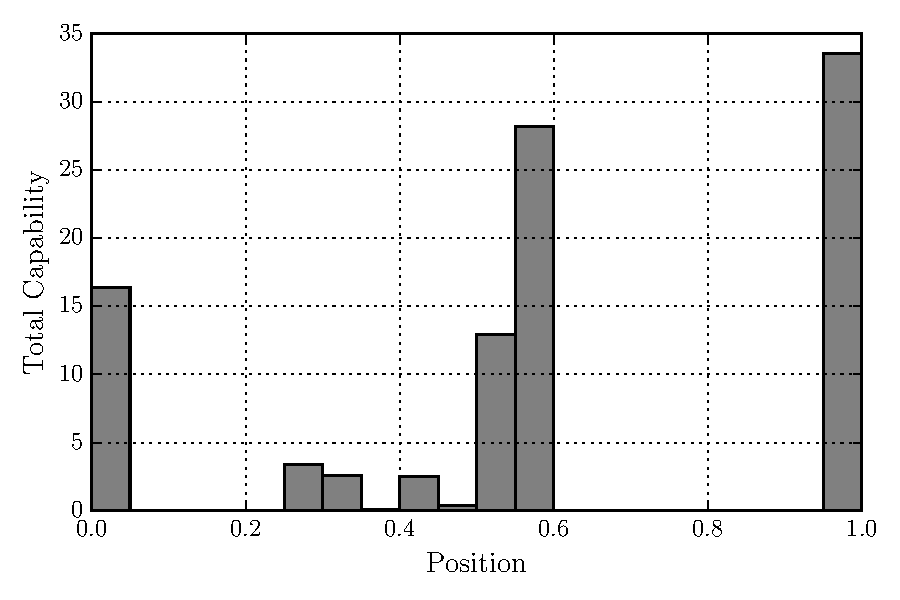
\includegraphics[scale=0.75]{ColdWar/Figures/Updated_Inputs_hist}
  \caption[Updated Inputs]{Updated Inputs - Initial Distribution of Capabilities}
  \label{fig:updated_input_hist}
  \figSpace
 \end{figure}

\begin{landscape}
\begin{table}
  \centering
  \caption{Updated Inputs}
  \label{table:new_inputs}
  \begin{tabular}{lcc||lcc||lcc}
  \hline
  Country            & Capability & Position & Country     & Capability & Position & Country                  & Capability & Position \\
  \hline
Afghanistan        & 0.23       & 0.58     & Haiti       & 0.04       & 0.98     & Paraguay                 & 0.04       & 0.98     \\
Albania            & 0.09       & 0.36     & Honduras    & 0.02       & 0.98     & Peru                     & 0.17       & 0.98     \\
Argentina          & 0.82       & 0.98     & Hungary     & 0.41       & 0.30     & Philippines              & 0.33       & 0.56     \\
Australia          & 0.83       & 0.57     & Iceland     & 0.00       & 0.56     & Poland                   & 2.98       & 0.30     \\
Belgium            & 1.09       & 0.42     & India       & 5.23       & 0.56     & Portugal                 & 0.26       & 0.46     \\
Bolivia            & 0.06       & 0.98     & Iran        & 0.43       & 0.51     & Romania                  & 0.55       & 0.34     \\
Brazil             & 1.22       & 0.98     & Iraq        & 0.13       & 0.49     & Russia                   & 16.36      & 0.00     \\
Bulgaria           & 0.31       & 0.42     & Ireland     & 0.10       & 0.56     & Saudi Arabia             & 0.11       & 0.59     \\
Canada             & 1.26       & 0.56     & Israel      & 0.14       & 0.56     & South Africa             & 0.52       & 0.56     \\
Chile              & 0.20       & 0.98     & Italy       & 1.92       & 0.56     & Spain                    & 1.48       & 0.57     \\
China              & 11.48      & 0.57     & Jordan      & 0.02       & 0.52     & Sri Lanka                & 0.09       & 0.56     \\
Colombia           & 0.26       & 0.98     & Lebanon     & 0.03       & 0.59     & Sweden                   & 0.60       & 0.56     \\
Costa Rica         & 0.01       & 0.98     & Liberia     & 0.01       & 0.56     & Switzerland              & 0.20       & 0.56     \\
Cuba               & 0.17       & 0.98     & Luxembourg  & 0.29       & 0.42     & Syria                    & 0.09       & 0.59     \\
Czechoslovakia     & 1.26       & 0.34     & Mexico      & 0.66       & 0.98     & Thailand                 & 0.34       & 0.56     \\
Denmark            & 0.21       & 0.56     & Mongolia    & 0.04       & 0.57     & Turkey                   & 1.17       & 0.51     \\
Dominican Republic & 0.06       & 0.98     & Myanmar     & 0.23       & 0.56     & United Kingdom           & 7.52       & 0.54     \\
Ecuador            & 0.09       & 0.98     & Nepal       & 0.11       & 0.56     & United States of America & 29.39      & 1.00     \\
Egypt              & 0.54       & 0.52     & Netherlands & 0.83       & 0.42     & Uruguay                  & 0.08       & 0.98     \\
El Salvador        & 0.03       & 0.98     & New Zealand & 0.09       & 0.57     & Venezuela                & 0.13       & 0.98     \\
Ethiopia           & 0.23       & 0.56     & Nicaragua   & 0.01       & 0.98     & Yemen Arab Republic      & 0.06       & 0.59     \\
Finland            & 0.19       & 0.57     & North Korea & 0.36       & 0.56     & Yugoslavia               & 0.80       & 0.32     \\
France             & 3.25       & 0.51     & Norway      & 0.16       & 0.56     &                          &            &          \\
Greece             & 0.36       & 0.56     & Pakistan    & 1.18       & 0.56     &                          &            &          \\
Guatemala          & 0.07       & 0.98     & Panama      & 0.01       & 0.98     &                          &            &   \\      
  \hline
\end{tabular}

  \tableSpace
\end{table}
\end{landscape}

%% [WGK]: 2. ... Related, Table 2.3, has numbers with apparently 2, 3, and 5 significant figures. How to they interact and what would the histogram tell us?
  % --> DONE

\subsection{Model Instantiations} \label{models}

I use the input datasets above to instantiate two model variants, drawn from the previous chapter's Section 3.7.3. The first corresponds to Model 1a, and is the attempt to reproduce the original EUM as originally described across multiple papers \citep{bdm_1994,bdm_1997,bdm_2002}; I will refer to this as the Baseline model. The second corresponds to Model 2b, chosen because it was the most predictive of the ICEWS events in the previous chapter; I will refer to this as the Updated model.

These model variants differ from the versions in the previous chapter in their salience updating sub-model. As \citet{bdm_1998} notes, there are countless unpredictable elements affecting how states will perceive, and act on, their international security interests in the context of the Cold War, from domestic political changes to natural disasters. Rather than extend the model to explicitly capture more and more of these factors, we implicitly incorporate them by randomizing agent salience values. At the beginning of each step of the model, each agent's salience is randomly drawn from a uniform distribution over the ${[0, 1]}$ range -- this is salience sub-model variant $\mathbf{S_{1,1}}$, in the notation presented in the previous chapter. Since capability is always multiplied by salience, this effectively adds a noise factor to the agents' strength as well. While agents with greater capabilities are likely to remain stronger than ones with lower capabilities, there exist configurations of salience values under which the generally weaker agent temporarily has an advantage over a stronger agent.

% RAX: Can [the previous paragraph] be justified in any way? 
% Not that I know of? 

In the notation introduced in the previous chapter, these models can be denoted as:

\begin{description}
  \item[Baseline:] $\{\mathbf{T_0, S_{1,1}, W_0, R_0, O_0, M_0, A_0}\}$ 
  \item[Updated:] $\{\mathbf{T_1, S_{1,1}, W_1, R_1, O_0, M_1, A_0}\}$
\end{description}

Taken together, the two model variants and two input datasets yield four experiments in all, as shown in Table \ref{table:experiment_matrix}.

\begin{table}
  \centering
  \caption{Experiment Summary}
    \label{table:experiment_matrix}
  \begin{tabular}{l|cc}
  \hline
                & Baseline Model &  Updated Model \\
  \hline
  Original Inputs & Experiment 1   & Experiment 2   \\
  Updated Inputs  & Experiment 3    & Experiment 4  \\
  \hline
\end{tabular}
    \tableSpace
\end{table}

For all experiments, I instantiate all agents with parameters $Q=0.5$ and $T=0.5$ indicating maximum uncertainty about the world. Each model is run for 25 steps. \citet{bdm_1998} hypothesizes that this is roughly equivalent to 50 years of history, meaning that agents experience salience shocks, engage in conflicts, and change position approximately once every two years. With 1948 as the starting year, the models will generate data corresponding approximately to 1998 as the end year.

To briefly restate the model: during each step, each agent evaluates its expected utility from threatening conflict against each other agents in an attempt to coerce the other agents to adopt its current position; when that expected utility is positive, the agent issues the threat. The agents then evaluate all their incoming threats, choosing the one requiring the least movement, and moving based on their own expected utility (interpreted here as fear of a conflict), either compromising and moving slightly towards the threat sender's position or capitulating and adopting that position outright. In the Baseline variant, but not the Updated one, if agent A chooses B's threat, while B chooses C's threat, B backs out of its decision and does not move. 

If two agents threaten each other and do not choose to compromise with or capitulate to another agent, they enter into a conflict. All agents then contribute capability to the side they prefer, in proportion with the strength of their preference. The winner is chosen randomly, with probabilities based on each agent's share of total capability contributed to the conflict. In the Baseline variant, the loser of a conflict adopts the winner's position; in the Updated variant, neither agent changes position, regardless of the conflict outcome.

Due to the large number of independent random variables driving the model, I run 1,000 instantiations of each experiment. This number appears to be  sufficiently large to sample from the many different possible configurations of saliences and conflict outcomes\footnote{excursions using 10,000 instantiations did not produce meaningfully different outcome distributions.}. Furthermore, since we are concerned with commonly-emerging outcomes and behaviors, particular phenomena occurring less frequently than in 0.1\% of model runs are unlikely to be of practical interest.

%% [WGK] 1. Between the inputs and outputs, I suggest a little review of the processing of the model and possibly whether each round, representing ~2yrs, includes all agents making offers, etc. Related, are there any in process indicators other than the resulting overall positions, such as a track of an individual country’s relationship with the US and USSR? Jumping from inputs to outputs with no discussion of the process in between is uncomfortable.
  % --> DONE!


\subsection{Output Data} \label{outputs}

Each model run generates several outputs. At the beginning of each step of the run, it records the position currently held by each agent, as well as the current median voter position, and capability-weighted mean position. During each step, the model also logs all conflicts which occur between agents. I collect and aggregate these outputs across all 1,000 runs of each experiment.

I then compare these outputs to two Correlates of War datasets: militarized interstate disputes (MIDs) for the 1948-1998 timeframe, and alliance data for 1998. The MID dataset provides an expert-coded listing of all cases where one state threatened or used force against another \citep{jones_1996}. While there are many forms of conflict, militarized disputes, which can escalate into wars, are particularly important to the international system, and thus of particular interest for forecasting. I will attempt to see whether the number of conflict events between pairs of actors generated by the model runs is a useful predictor of the number of conflicts between states in the relevant time period. 

Similarly, the model runs produce traces of agent positions. Agents with closer positions are more likely to support one another more strongly in conflict with other agents, i.e. they behave the way we would expect allied countries to behave. Thus, I will test whether the distance between agents is a predictor of alliances between the corresponding countries.

\section{Results} \label{results}

\subsection{Overview}

The initial question posed by \citet{bdm_1998} was whether the end of the Cold War -- that is, a substantial shift in the median international security position to the advantage of the United States -- could be generated from the model. Figure \ref{fig:original_cdf} shows the cumulative distribution of model end positions reported by that paper. Note the sharp increase in the cumulative distribution curve very close to 0 (equivalent to 0.5, in the variant used here), indicating that one of the most common types of outcomes is one where the Cold War persists at the end of the model run, with a median position between the starting position of both superpowers and no clear advantage to either side. However, the distribution is also clearly non-symmetric, with more outcomes favoring the United States (closer to +100) than the USSR. The conclusion of the original paper was thus that the end of the Cold War, with an American victory, was not as unforeseeable as others had argued, and in fact could be emerged from the model.

\begin{figure}[h!]
  \centering
  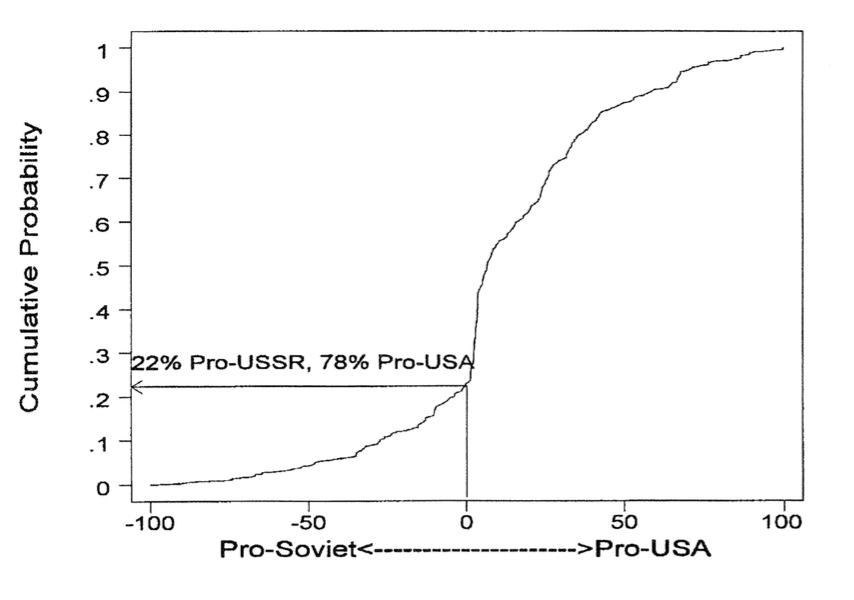
\includegraphics[scale=0.75]{ColdWar/Figures/ColdWarOriginal}
  \caption[Original Model Cumulative Distribution]{Model Outcome Cumulative Distribution, Copied From \citet{bdm_1998} }
  \label{fig:original_cdf}
  \figSpace
 \end{figure}

Figure \ref{fig:new_cdfs} shows the same cumulative distributions across the four experiments\footnote{\citet{bdm_1998} does not provide all the results of each model run, meaning that we cannot directly superimpose the results shown in Figures \ref{fig:original_cdf} and \ref{fig:new_cdfs}.}. Immediately, we note that the overall shapes are similar, though not identical. The bulk of outcomes are very close to the center, with substantially more US-victory outcomes than USSR-victory ones. In particular, Experiment 1, which attempts to replicate the original model, has almost no USSR-victory outcomes, and more outcomes where the median position does not indicate a victory to either side.

\begin{figure}[h!]
  \centering
  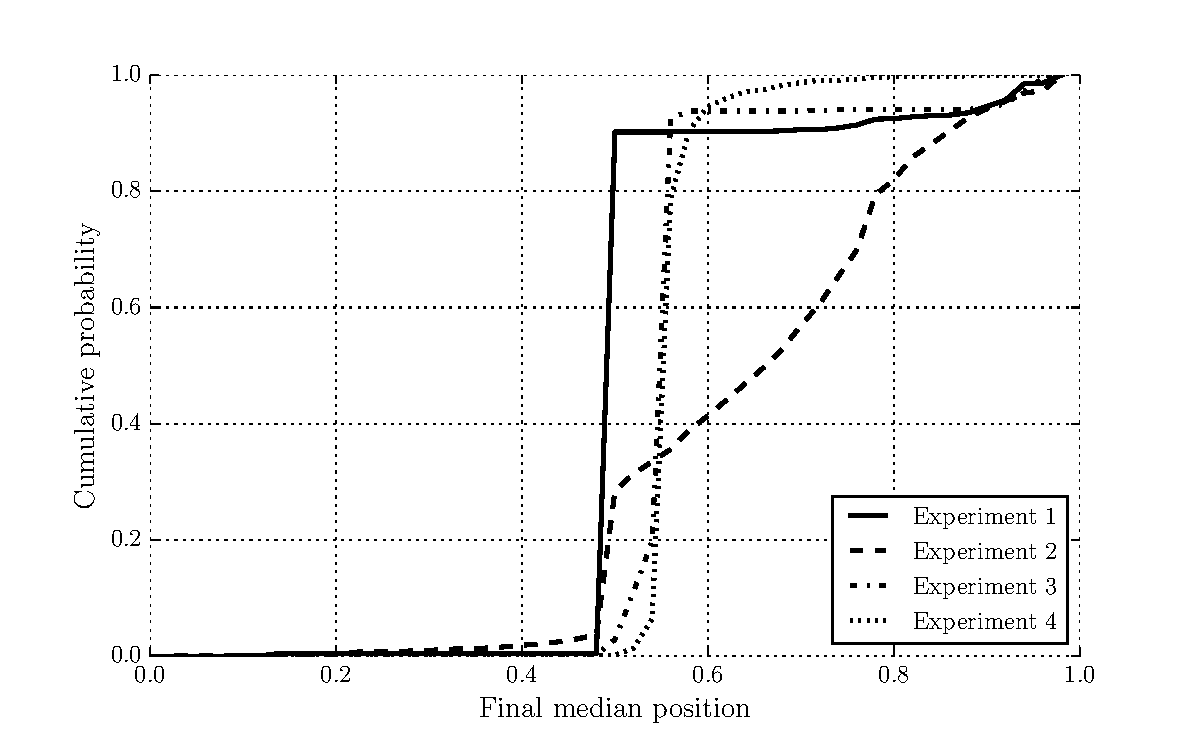
\includegraphics[scale=0.5]{ColdWar/Figures/Model_cdfs}
  \caption[New Model Cumulative Distribution]{Model Outcomes Cumulative Distributions}
  \label{fig:new_cdfs}
  \figSpace
 \end{figure}


%% [WGK] 3. Can Figure 2.3 (or an additional figure prior to 2.3) show us the range of values from all the runs rather than just the mean? Either standard error bands or all the runs plotted on top of each other?



\begin{figure}[t!]
    \centering
    \begin{subfigure}[t]{0.49\textwidth}
        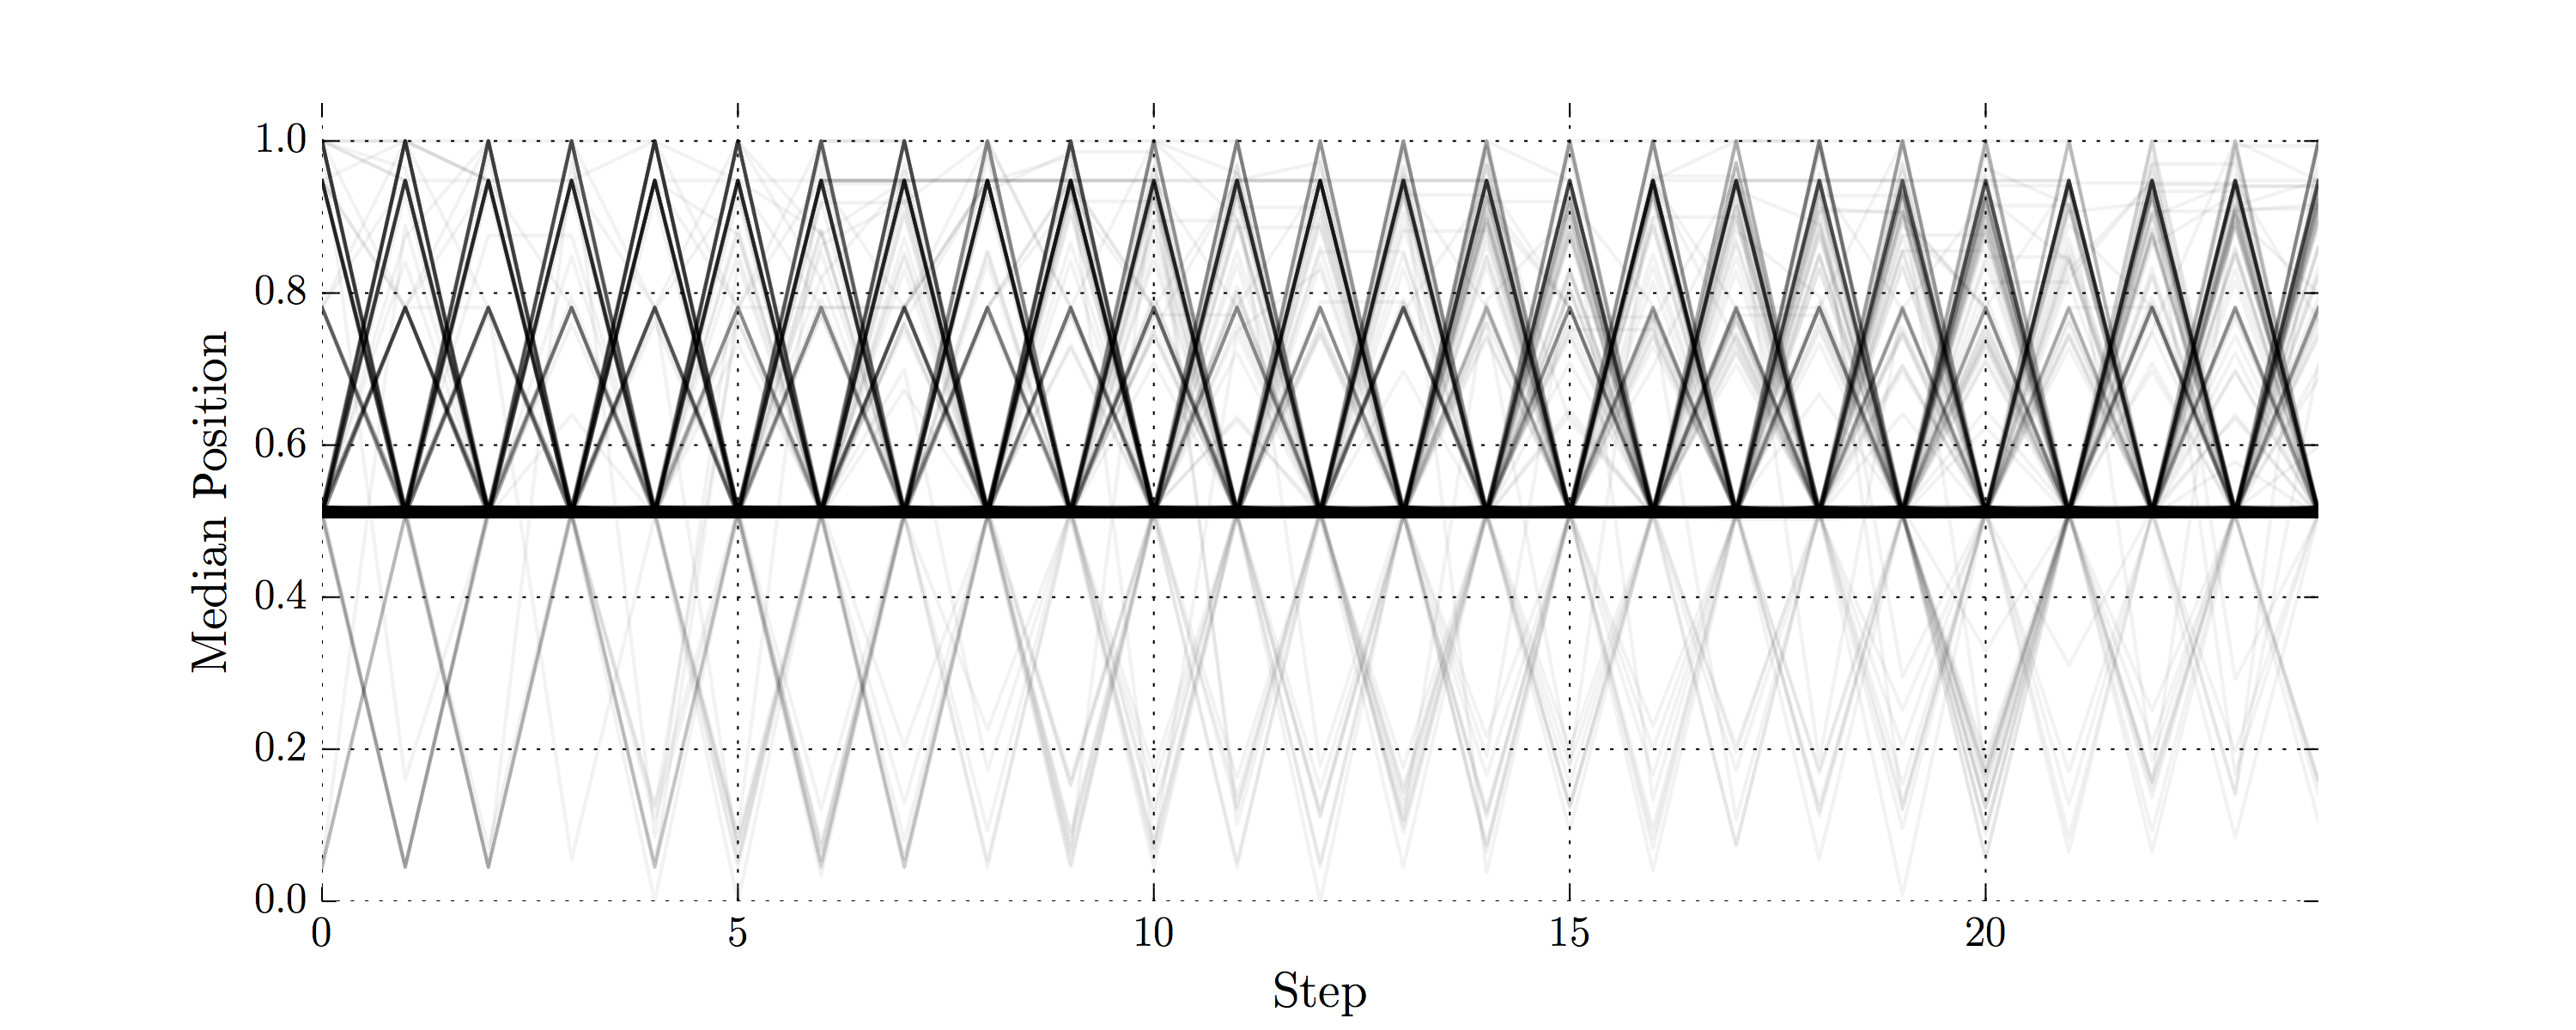
\includegraphics[width=\textwidth]{ColdWar/Figures/Exp1_traces}
        \caption{Experiment 1}
    \end{subfigure}
    \begin{subfigure}[t]{0.49\textwidth}
        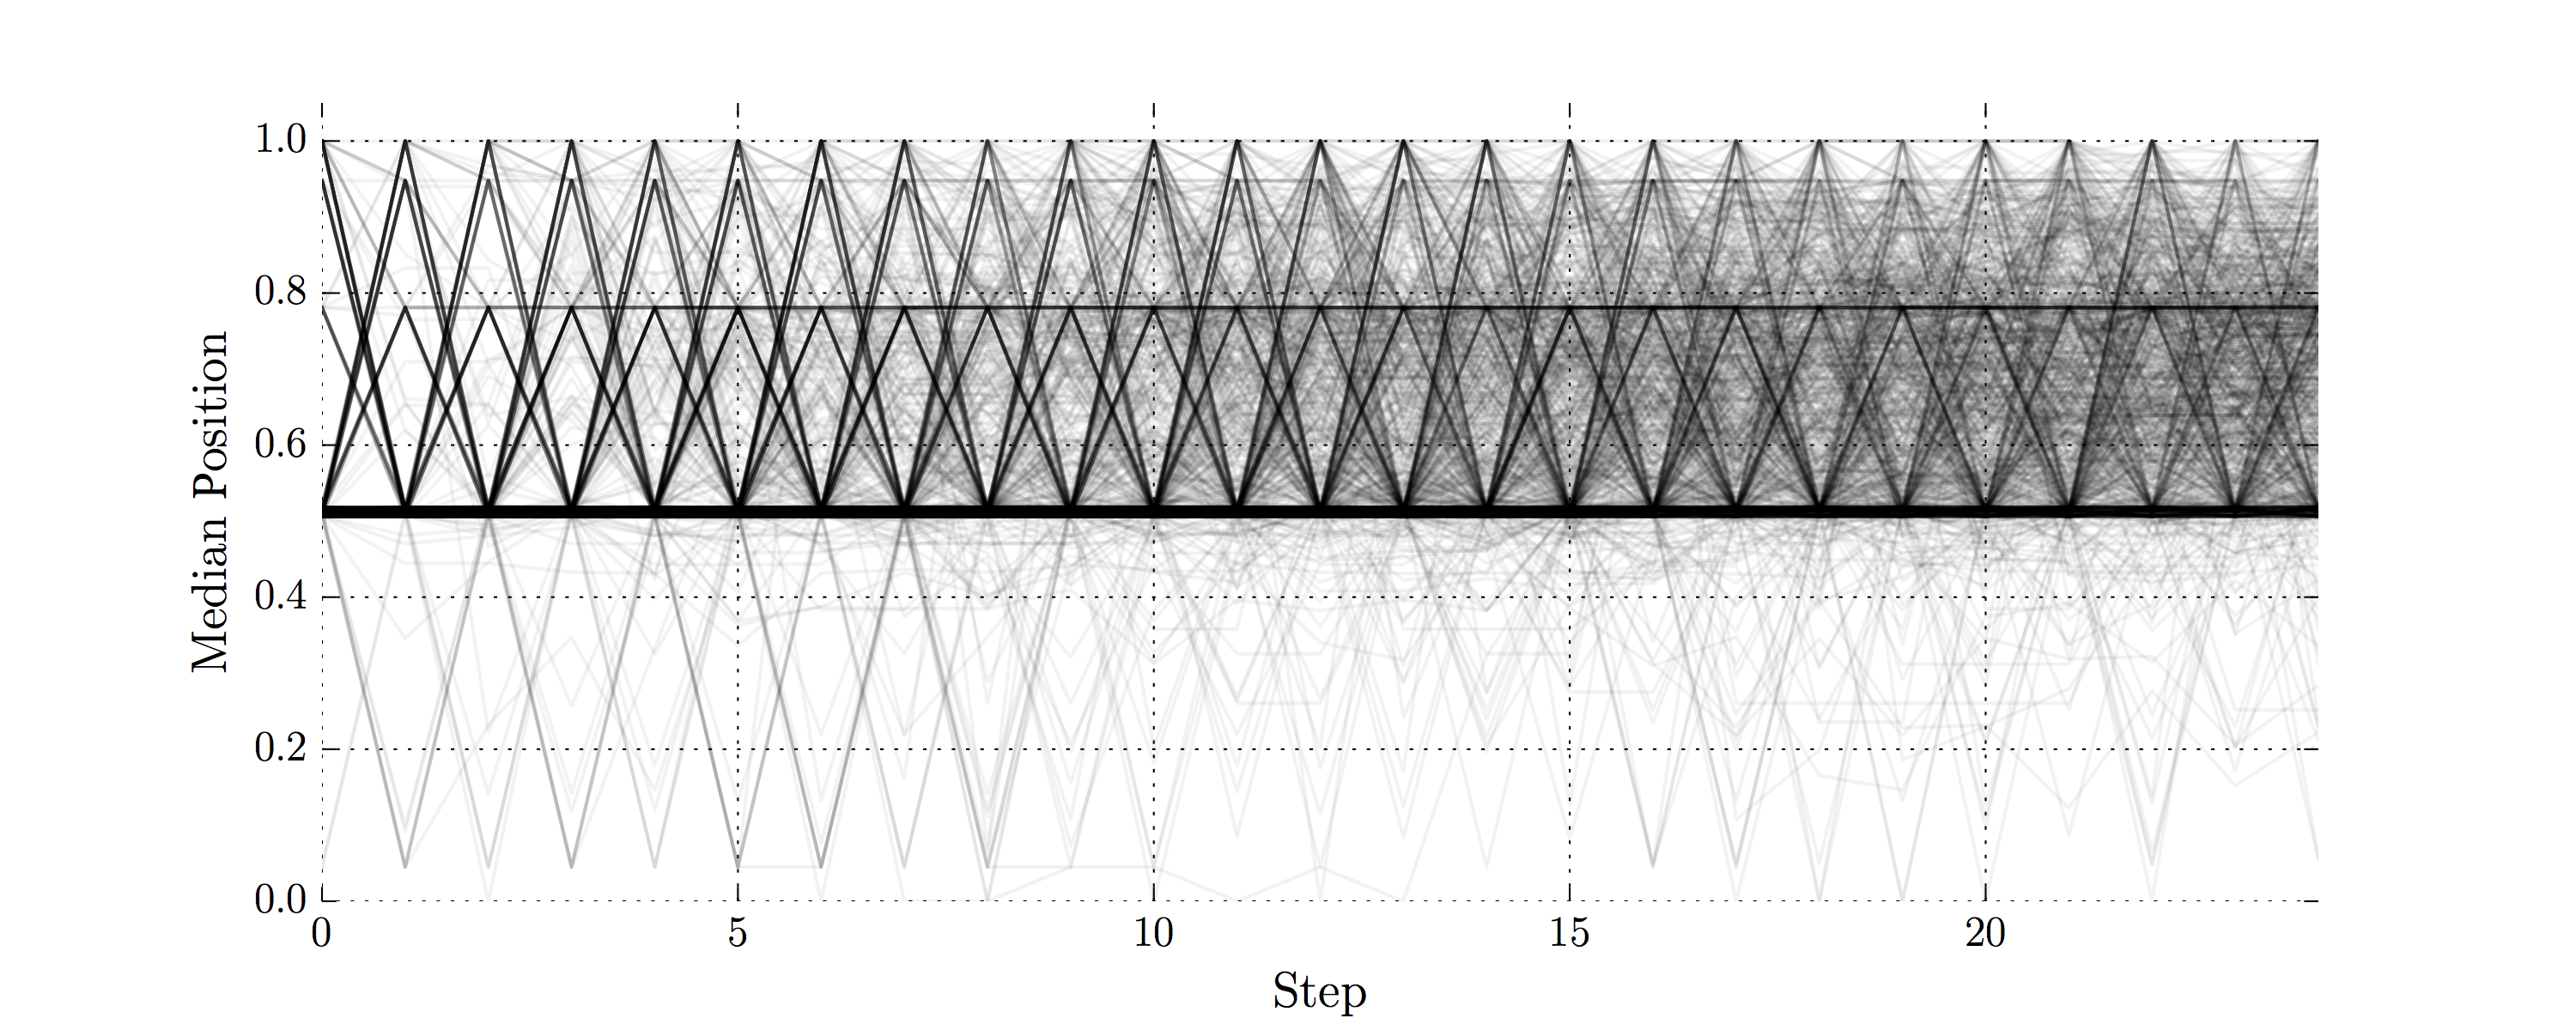
\includegraphics[width=\textwidth]{ColdWar/Figures/Exp2_traces}
        \caption{Experiment 2}
    \end{subfigure}

    \begin{subfigure}[t]{0.49\textwidth}
        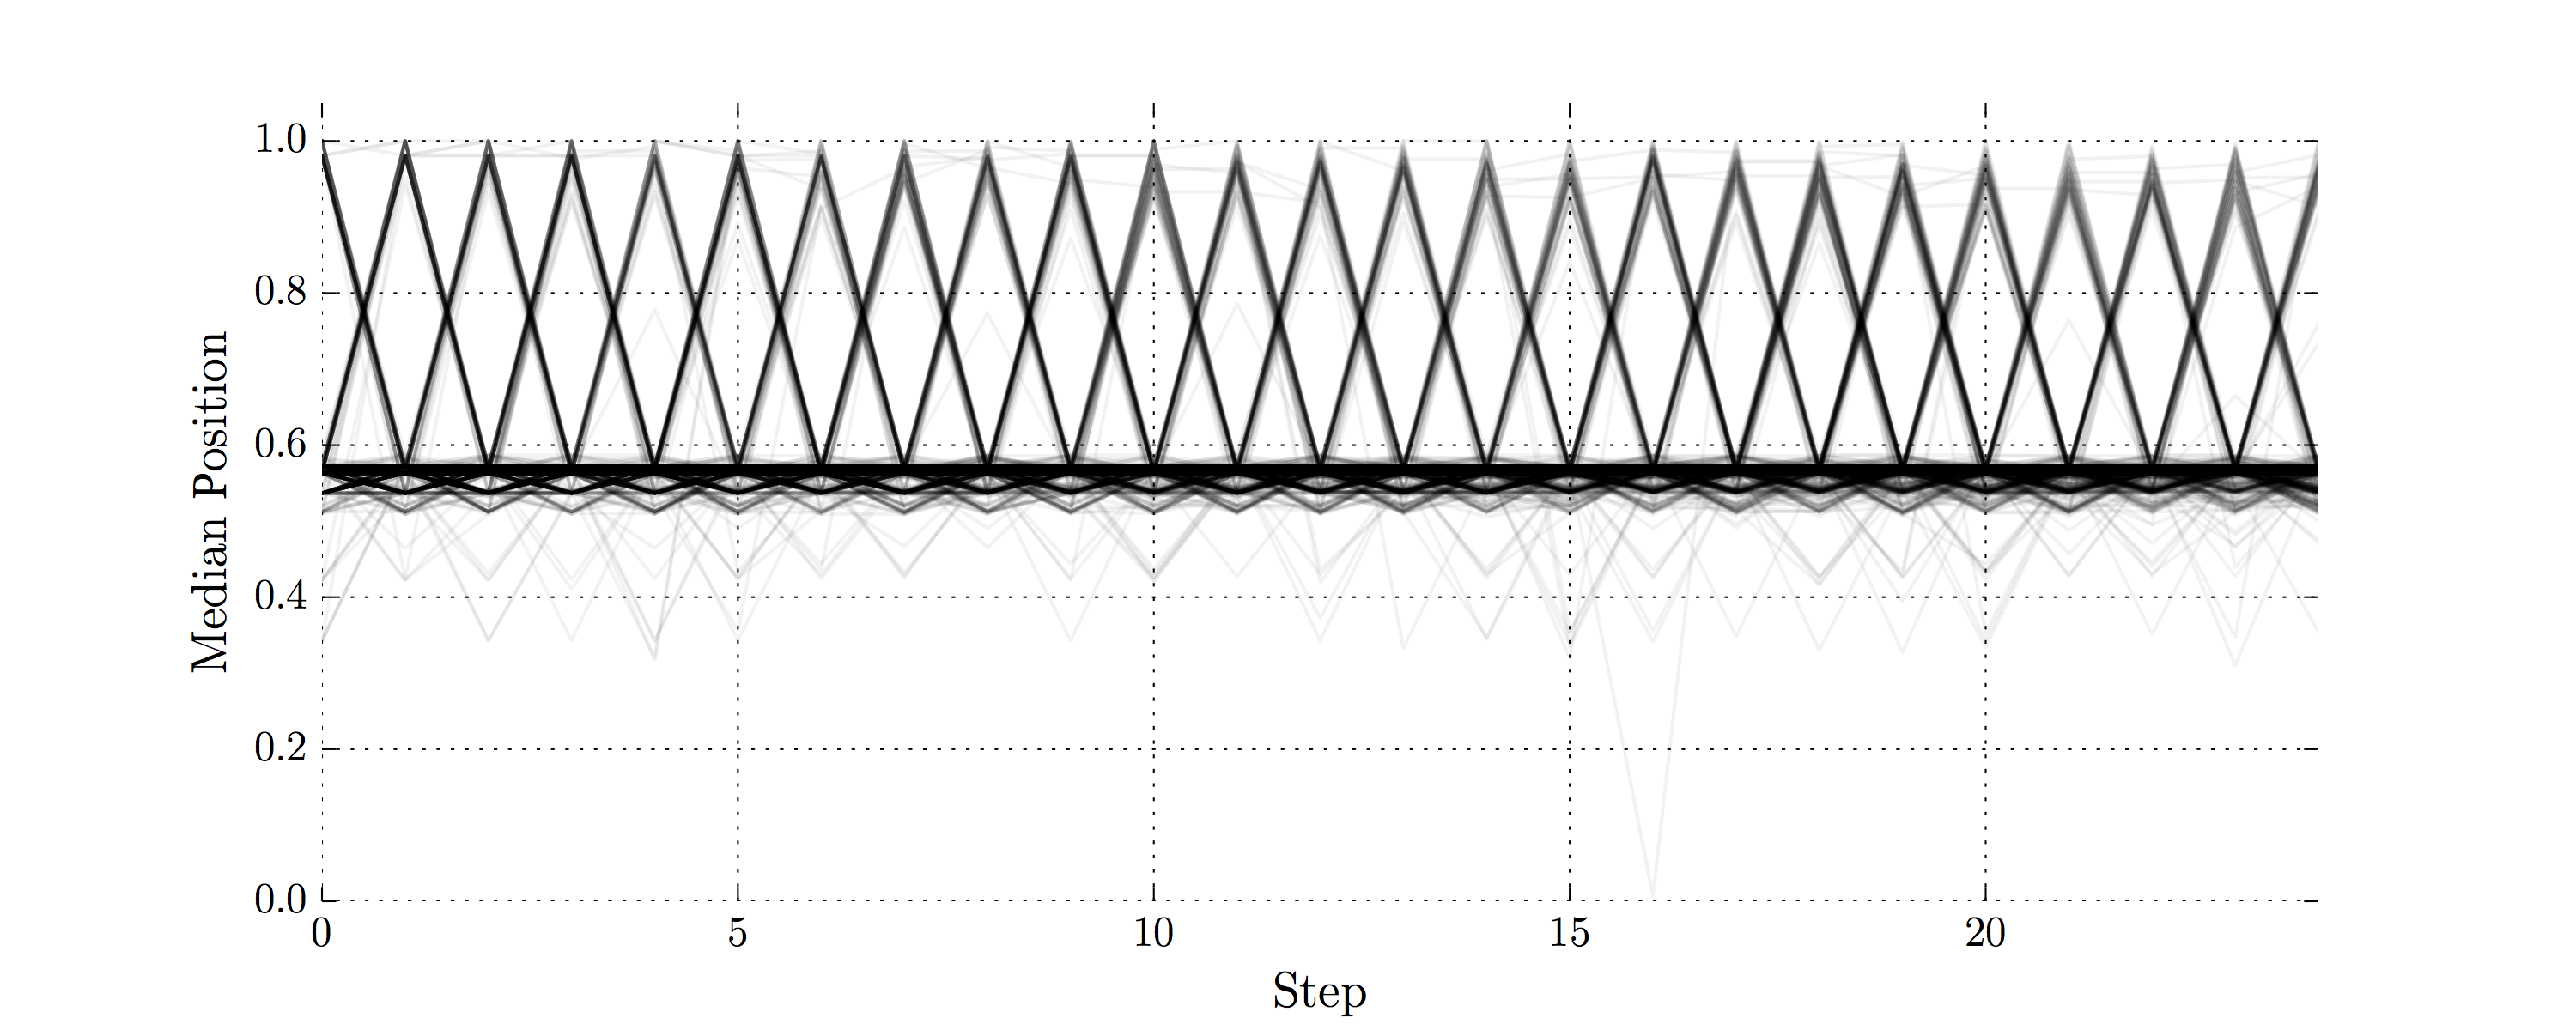
\includegraphics[width=\textwidth]{ColdWar/Figures/Exp3_traces}
        \caption{Experiment 3}
    \end{subfigure}
    \begin{subfigure}[t]{0.49\textwidth}
        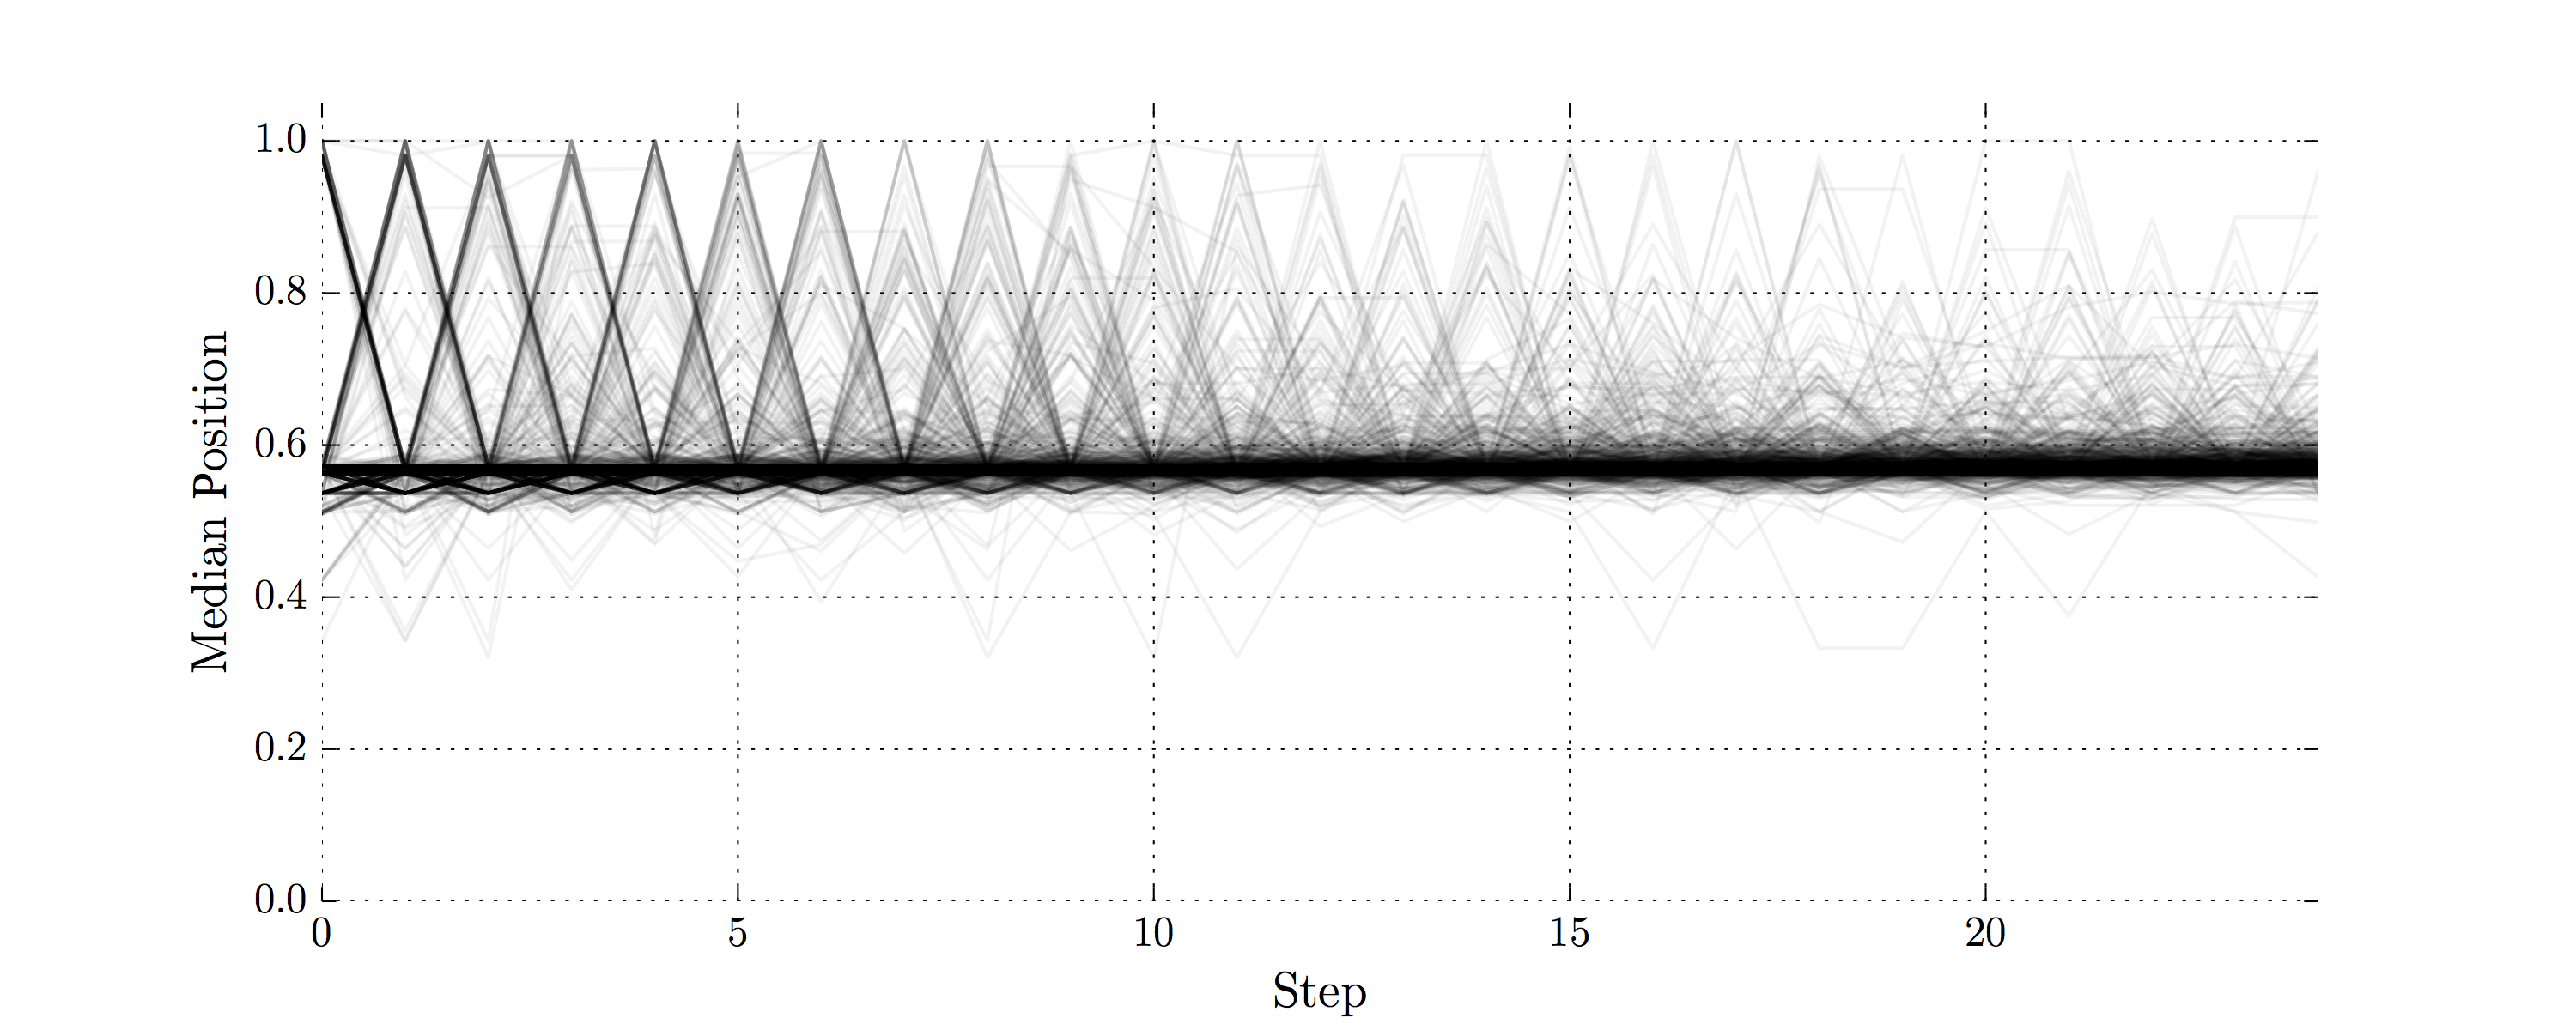
\includegraphics[width=\textwidth]{ColdWar/Figures/Exp4_traces}
        \caption{Experiment 4}
    \end{subfigure}
    
    \caption{Median Position Traces}
    \label{fig:model_traces}
    \figSpace
\end{figure}

%% [WGK] 4. There’s a description of the results as a sawtooth pattern before figures 2.4 are introduced. The reader can’t know where that comes from. <-- Make sure fig:model_traces appears before words 'sawtooth pattern'


Let us take a closer look at the behaviors these models are generating. Figure \ref{fig:model_traces} shows the superimposed traces of the median position for all the model runs of all experiments. The opacity of each trace line is low, so that the darker a line appears, the more traces exhibited that particular transition. While it is impossible to discern individual runs here, these visualizations serve to highlight recurring patterns. Two patterns are obvious across all four experiments. The first is that, as the cumulative distributions in Figure \ref{fig:new_cdfs} suggest, the most common positions for the model at any given step are at or close to the starting median -- by and large, the median does not change very often. The next key pattern is that, across all the experiments, the median position exhibits a sawtooth pattern, diverging from the 0.5 position towards one extreme or the other and immediately returning. In other words, one of the sides (though more frequently the United States) gains a brief advantage, and then the status quo quickly reasserts itself. This sawtooth pattern is particularly distinct and uniform in the Baseline model used in Experiments 1 and 3. Experiment 2, and to a lesser extent Experiment 4, show a wider variety of traces. In particular, close examination of the Experiment 2 traces indicates more cases where changes in median are not one-round spikes, but transitions to a new stable position. Finally, Experiment 4 shows a decline in movement as time advances, suggesting that the agents are sorting themselves into a more stable configuration around the same median.

The sawtooth pattern raises a question: do the model runs ending in a US (or Soviet, for that matter) victory represent a true long-term shift in the status quo, or are they simply cases where a temporary spike towards one side or the other coincides with the final step of the model? In fact, a close examination of the model runs suggests that the latter is exactly what is happening in Experiments 1 and 3. Figure \ref{fig:example_traces} shows example traces from randomly-selected runs which end with a median position of 0.7 or greater, indicating a US victory. In the traces from Experiments 1 and 3, the median position exhibits several short-lived excursions away from the baseline position, quickly reverting after each. There is no reason to suppose that the spike preceding the end of the run represents a true change from this pattern. The trace from Experiment 2, in contrast, shows that the median position had gone up prior to the final step of the run, and remained relatively stable at its new position. The Experiment 4 trace also shows the run achieving a new stable position, with smaller spikes away from it, including one coinciding with the terminal step. These patterns recur across the runs in each experiment that are not visualized here, including those not ending in a US victory.

A thorough examination of model runs suggests that the spikes -- including the terminal ones -- are driven less by changes in agent positions than by the changes of agent salience values. Importantly, these changes are not accompanied by a similar change in the weighted mean position -- which is to say, not driven by similar changes in the positions of the agents themselves. Recall that as detailed in the previous chapter, in Section 3.2.2, the median is computed by checking which agent position has the highest probability of defeating all other agent positions in bilateral conflicts; thus, they are affected by the stochastic salience changes. In contrast, the mean position is weighted by (fixed) capabilities, and thus is not directly affected by salience variations.

This phenomenon is illustrated in Figure \ref{fig:example_agent_traces}, showing the individual agent positions over time for the same runs as in Figure \ref{fig:example_traces}. In this figure, each line corresponds to an agent: the $y$ axis indicates each agent's position at each step, shown on the $x$ axis; line widths correspond to the agents' capabilities. The top-most line is always the position of the United States agent and the bottom-most line is the USSR agent. The traces for all the experiments show that the radical, temporary spikes in the median position do not correspond to similar sharp shifts in any agent position. In Experiment 1, the agents exhibit a slight movement towards the center of the position space. Note, however, that the movement by the USSR agent and its allies (at the bottom of the graph) are more substantial than those of the US and its aligned agents at the top. In Experiment 3, however, very little movement occurs at all. In Experiments 2 and 4, in contrast, the agents exhibit sharp, more substantial changes in their positions, which correspond to the changes in the median, highlighting that the median change is not being driven solely here by stochastic changes in salience.

In fact, in the Experiment 2 and 4 traces, we can see a particularly interesting story emerge. Early on, several agents whose positions are closer to the median are drawn closer to the position of the United States; this is followed by several Soviet-aligned agents being drawn `upward' towards the United States's preferred position across multiple steps. The Soviet Union itself lags behind these agents for a number of steps. However, eventually it too is driven to adjust its position upwards, in the Experiment 4 trace even eventually joining the US-aligned cluster. In effect, this model generates a recognizable notional history of the Cold War leading to a US-dominated unipolar world. 

\begin{figure}[!htbp]
    \centering
    \begin{subfigure}[t]{0.49\textwidth}
        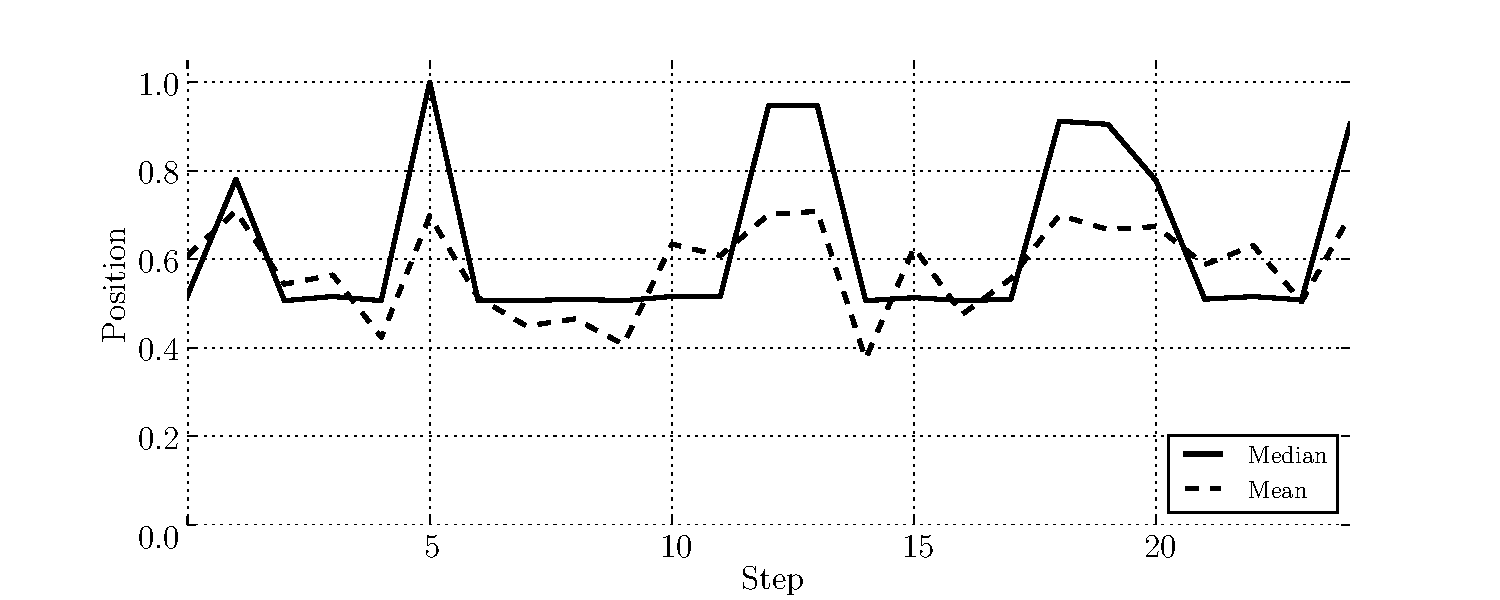
\includegraphics[width=\textwidth]{ColdWar/Figures/Exp1_uswin_trace}
        \caption{Experiment 1}
    \end{subfigure}
    \begin{subfigure}[t]{0.49\textwidth}
        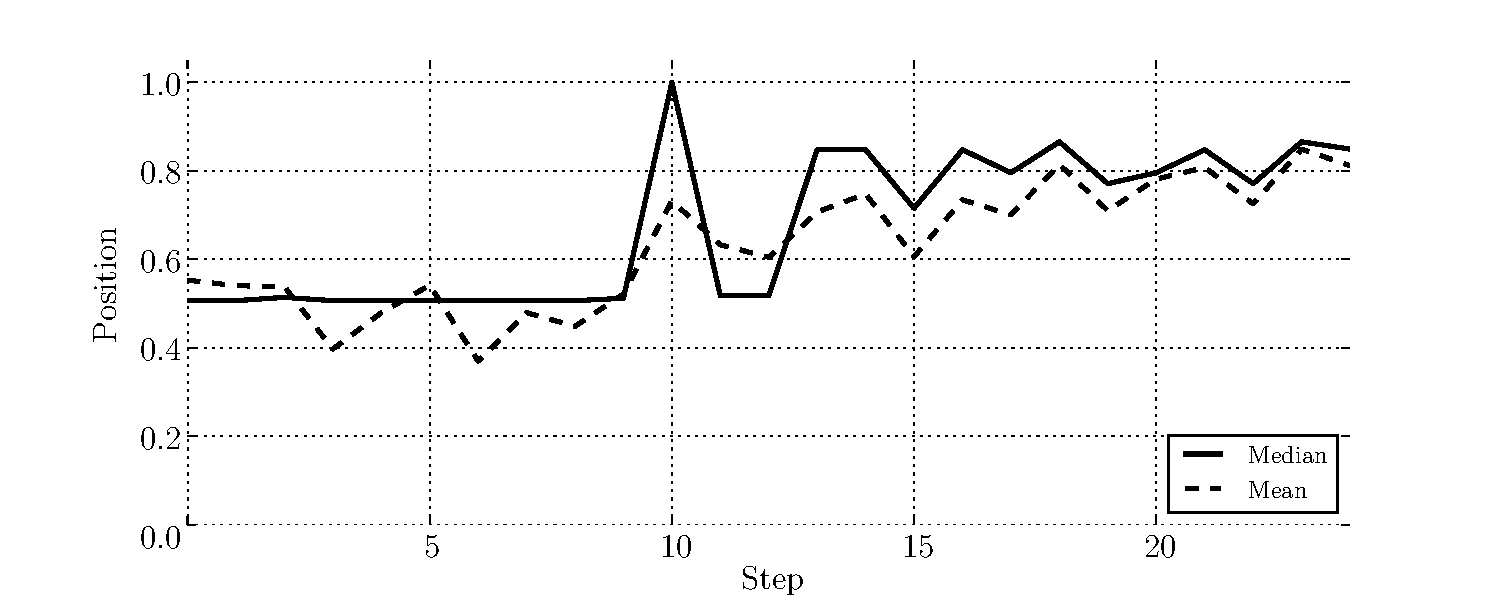
\includegraphics[width=\textwidth]{ColdWar/Figures/Exp2_uswin_trace}
        \caption{Experiment 2}
    \end{subfigure}

    \begin{subfigure}[t]{0.49\textwidth}
        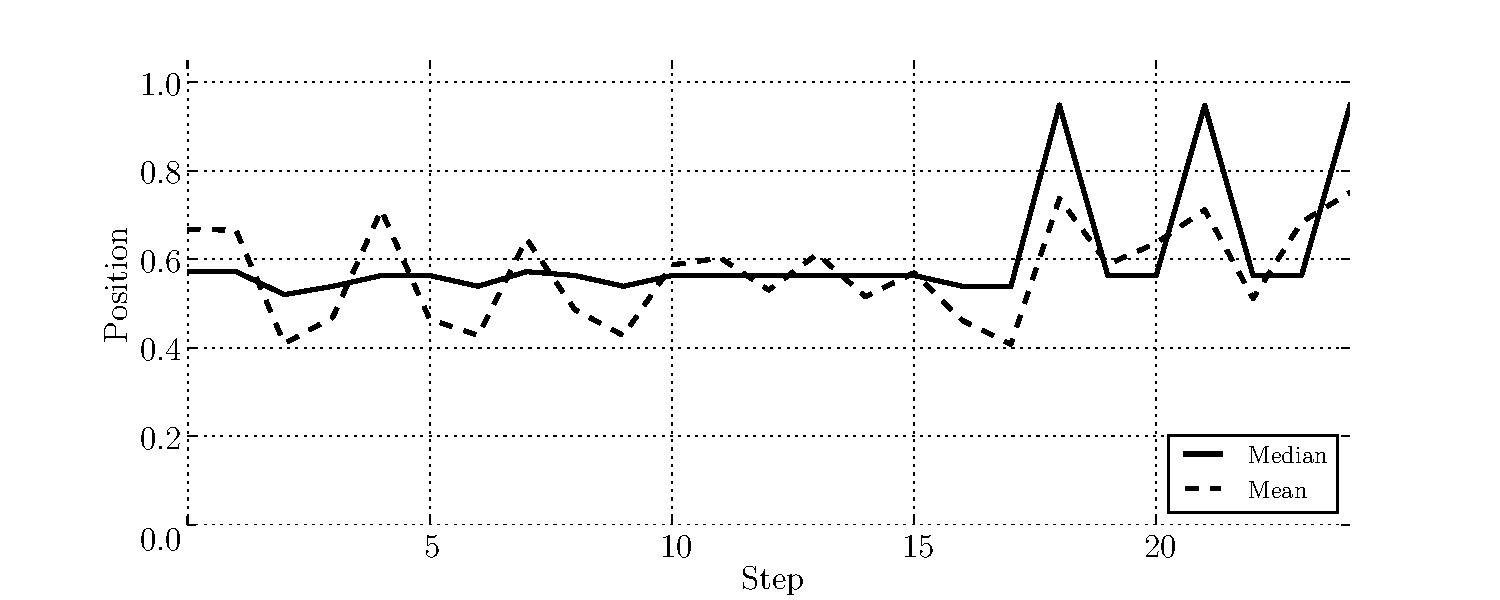
\includegraphics[width=\textwidth]{ColdWar/Figures/Exp3_uswin_trace}
        \caption{Experiment 3}
    \end{subfigure}
    \begin{subfigure}[t]{0.49\textwidth}
        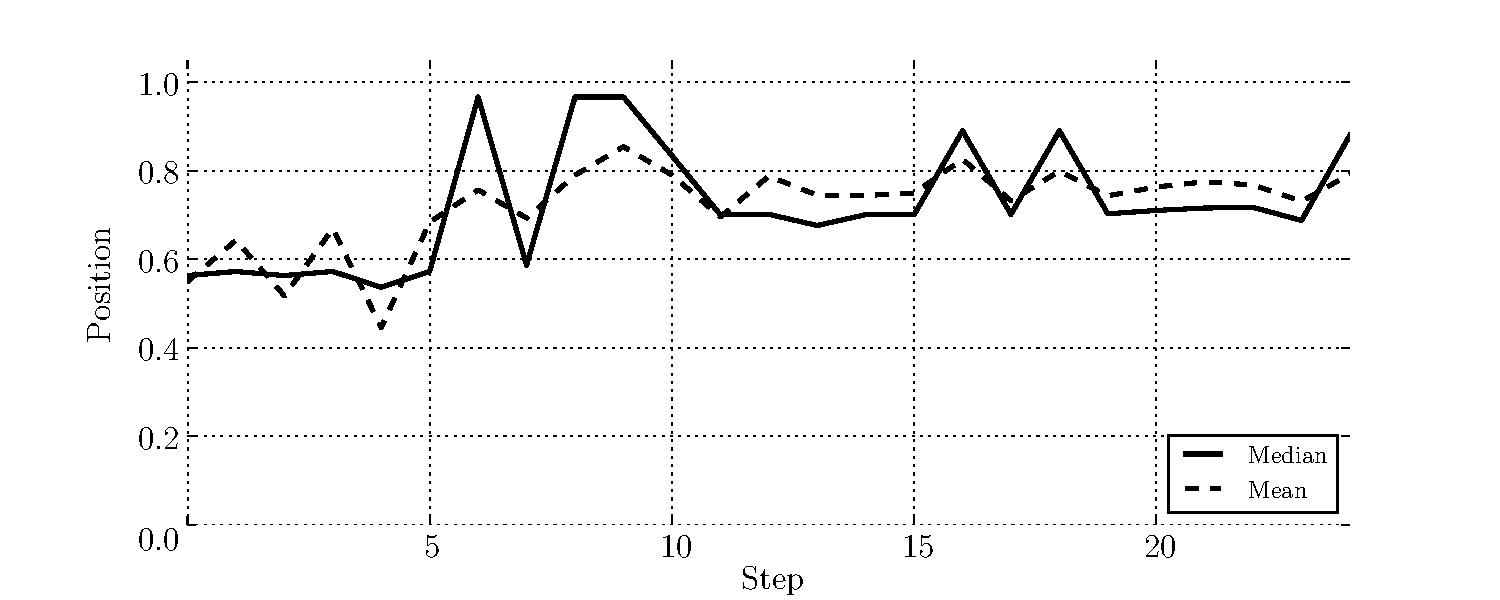
\includegraphics[width=\textwidth]{ColdWar/Figures/Exp4_uswin_trace}
        \caption{Experiment 4}
    \end{subfigure}

    \caption{Example Model Traces -- Median Positions}
    \label{fig:example_traces}
    \figSpace
\end{figure}

\begin{figure}[!htbp]
    \centering
    \begin{subfigure}[t]{0.75\textwidth}
        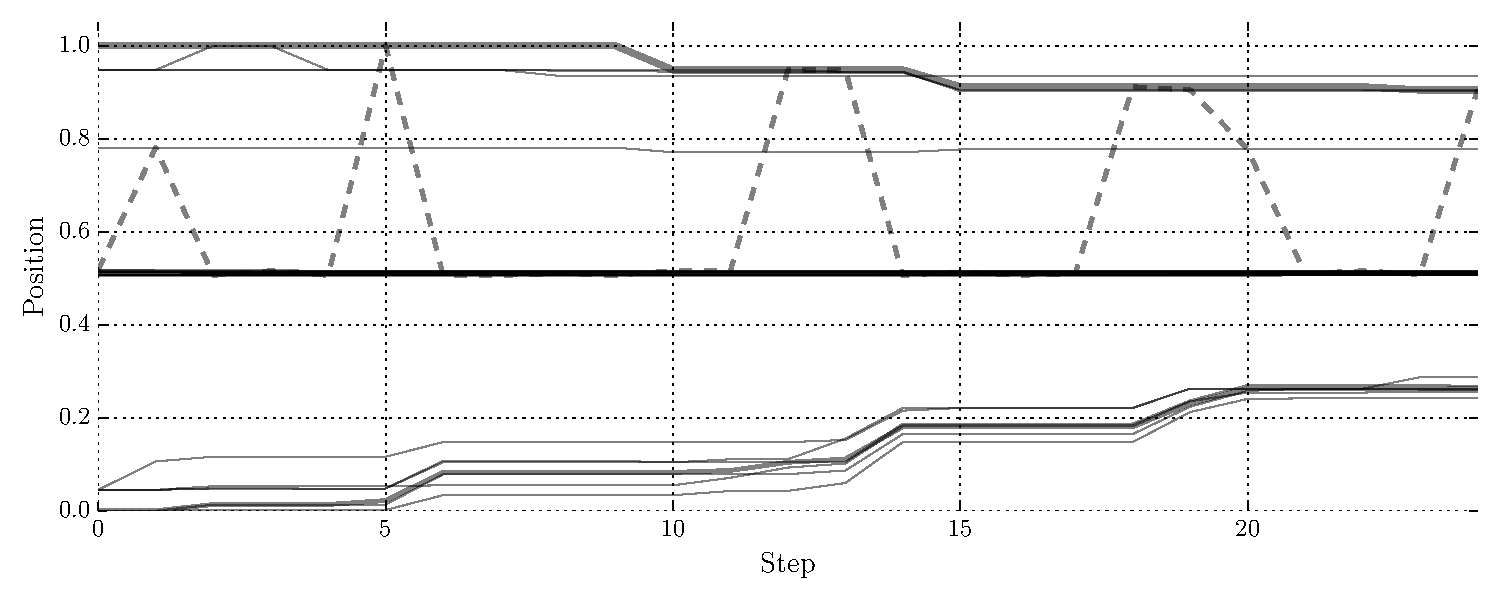
\includegraphics[width=\textwidth]{ColdWar/Figures/Exp1_agent_traces}
        \caption{Experiment 1}
    \end{subfigure}

    \begin{subfigure}[t]{0.75\textwidth}
        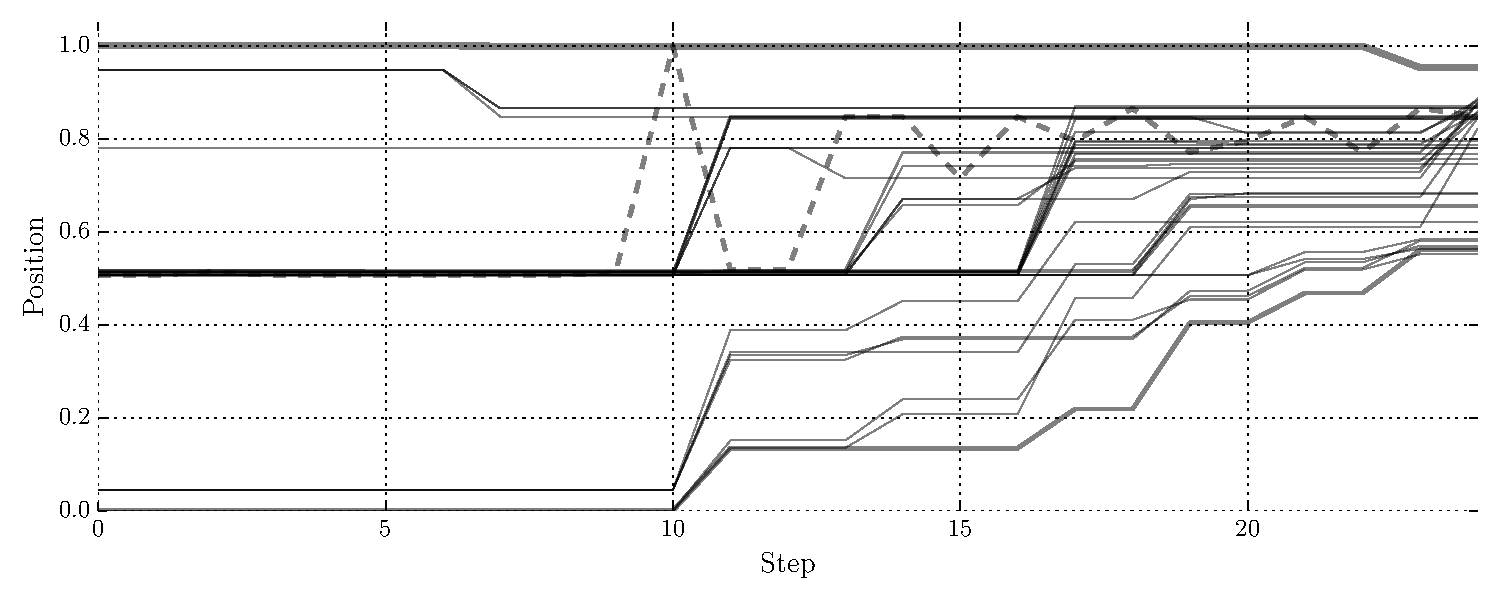
\includegraphics[width=\textwidth]{ColdWar/Figures/Exp2_agent_traces}
        \caption{Experiment 2}
    \end{subfigure}

    \begin{subfigure}[t]{0.75\textwidth}
        \includegraphics[width=\textwidth]{ColdWar/Figures/Exp3_agent_traces}
        \caption{Experiment 3}
    \end{subfigure}

    \begin{subfigure}[t]{0.75\textwidth}
        \includegraphics[width=\textwidth]{ColdWar/Figures/Exp4_agent_traces}
        \caption{Experiment 4}
    \end{subfigure}

    \caption{Example Model Traces -- Agent Positions}
    \label{fig:example_agent_traces}
    \figSpace
\end{figure}

\subsection{Predicted Conflicts}

The models do not only generate overall positional traces, but simulated events, and conflicts in particular. These conflicts are an important part of the simulated history, not only because they can drive substantial changes in agent positions but because they provide useful anchor-points for comparing model runs to real history. We have robust historic data on wars and lesser militarized interstate disputes, and a well-developed understanding of international partnerships and rivalries, which allow us to assess the plausibility of the conflicts the model produces. Furthermore, conflicts are an important area for prediction and forecasting, and it is valuable to assess whether these models can be used for such prediction.

Each model run in each experiment collects the conflict events generated across all run steps; for each, the code computes the mean number of conflicts occurring between each dyad of agents across all models. These dyads are undirected, since in the model variants applied here both parties must mutually decide to start a conflict for it to occur. These simulated conflict counts are then merged with the count of militarized interstate disputes for each dyad, as described above.

The correlations between the predicted and observed number of conflicts are small. Most conflicts generated by the model do not reflect real conflicts, while most real conflicts are not mirrored in the simulated data. Nevertheless, we may still ask whether the model provides any statistically useful information. In order to do so, I run two regressions on each experiment output, with predicted conflicts as the independent variable: a linear regression, with observed MIDs as the dependent variable, shown in Table \ref{table:mids_linear}; and a logistic regression, with a dependent dummy variable for the presence of any MIDs on the dyad, in Table \ref{table:mid_logits}. The model generates relatively few conflicts -- like real-world wars, these are rare events \citep{king_2001}, meaning that the mean conflicts values are small, leading to large-magnitude coefficients. 

First, let us examine the linear regressions. Note that we have no particular reason to believe that the relationship between the number of model-generated and observed conflicts is linear. However, if more simulated conflicts do in fact predict more observed conflicts, we would expect the coefficient to be positive. In fact, all the coefficients are positive, and all but the one for Experiment 1 are statistically significant, suggesting that the models are generating some useful information as to the number of observed conflicts.

Further evidence of this is visible in Table \ref{table:mid_logits}. These regressions test whether more model conflicts between dyads of actors predict \emph{any} conflicts occurring in the relevant time period. In this case the coefficient values are positive and significant across all the models, indicating that when the model predicts more conflicts between a pair of countries, we are indeed more likely to have observed at least one conflict between them in the historic data.

While $R^2$ is an imperfect measure of the goodness-of-fit of a statistical model, it is an acceptable way of comparing models of the same type and the same dependent variable \citep{wooldridge_2008}. The $R^2$ values across all models are low, indicating that they are explaining only a small fraction of the variance observed in the MID data. Nevertheless, we can see that the $R^2$ value on the Experiment 4 linear regression is an order of magnitude better than for the other experiments, and that this is not the case for the logistic regression. This suggests that the model is more accurately predicting the number of conflicts, conditional on conflicts occurring at all. Across both types of regressions, furthermore, we can see that Experiment 3 has the least explanatory power.


\begin{table}
  \begin{center}
  \caption{Militarized Interstate Disputes -- Linear Regressions}
  \label{table:mids_linear}
  \begin{tabular}{lcccc}

  \hline
                      & Experiment 1 & Experiment 2 & Experiment 3 & Experiment 4  \\
  \hline
  Const.               & 1.043***     & 1.014***     & 0.392***     & 0.362***      \\
                       & (0.183)      & (0.173)      & (0.049)      & (0.044)       \\
  Model Conflicts      & 1.473        & 8.327***     & 17.409***    & 1015.746***    \\
                       & (1.235)      & (1.950)      & (5.090)      & (40.768)     \\
  \hline
  Adjusted $R^2$     &     0.001      &   0.027      &  0.004       &   0.195 \\            
  \hline
  \hline
  \multicolumn{4}{l}{Standard errors in parentheses.} \\
  \multicolumn{4}{l}{* $p<.1$, ** $p<.05$, *** $p<.01$} \\
  \end{tabular}
  \end{center}
  \tableSpace
\end{table}

\begin{table}
  \begin{center}
  \caption{Militarized Interstate Disputes -- Logistic Regressions}
  \label{table:mid_logits}
  \begin{tabular}{lcccc}
  \hline
                      & Experiment 1 & Experiment 2 & Experiment 3 & Experiment 4  \\
  \hline
  Const.               & -1.300***    & -1.422***    & -2.201***    & -2.197***     \\
                       & (0.101)      & (0.111)      & (0.067)      & (0.066)       \\
  Model Conflicts & 1.952***     & 27.658***    & 19.739***    & 654.501***    \\
                       & (0.622)      & (7.190)      & (4.556)      & (148.758)     \\
  \hline
  McFadden's $R^2$     &  0.015       &  0.030       & 0.009        & 0.016 \\
  \hline
  \hline
  \multicolumn{4}{l}{Standard errors in parentheses.} \\
  \multicolumn{4}{l}{* $p<.1$, ** $p<.05$, *** $p<.01$} \\
  \end{tabular}
  \end{center}
  \tableSpace
\end{table}

It is also useful to look at the specific conflicts being predicted. Table \ref{table:conf_dyads} shows the top ten most frequently predicted conflict dyads for each experiment. One finding that stands out here is that the Baseline and Updated models appear to generate two different classes of conflcit. The Baseline model generates no direct conflicts between the two rival superpowers in either Experiment 1 or 3, and very few even directly involving either. Instead, the conflicts are largely between lower-tier agents, with positions closer to the median. In historic terms, these are proxy wars: the belligerents are not the superpowers themselves, but each draws some support from a different superpower and its close allies. These contributions are often small, as their preference for one side over the other may be relatively weak. The stakes of the conflicts, in terms of the overall orientation of the simulated international system, are correspondingly weak. In contrast, the Updated model sees much more direct involvement by the two main superpowers directly, including direct conflicts between them. The conflicts that are not between the two superpowers directly appear to often take the form of one superpower (most often the USA) attempting to coerce a much weaker country.

%Belgium is especially over-represented in the conflicts generated in both Experiments 1 and 3. This appears to be driven by its combination of relative strength and location close to the median (in Experiment 1, its own position is frequently the median position), making it a particularly influential actor in the simulated international system. In contrast, the Updated model generates many conflicts involving the USA and USSR agents, including frequent direct conflicts between the two.

\begin{table}
  \begin{center}
  \caption{Top Predicted Conflict Dyads}
  \label{table:conf_dyads}
  \begin{tabular}{l|l}
  \hline
  Experiment 1 & Experiment 2 \\
  \hline
  \begin{tabular}{ll}
  England & Iraq \\
  Egypt & England \\
  Belgium & France \\
  Belgium & Iran \\
  Argentina & USA \\
  Belgium & Egypt \\
  Argentina & Brazil \\
  Egypt & Iraq \\
  Belgium & Netherlands \\
  Argentina & Canada
  \end{tabular} & \begin{tabular}{ll}
    Bulgaria & USA \\ 
    USSR & USA \\ 
    USA & Yugoslavia \\ 
    China & USA \\ 
    England & USSR \\ 
    Australia & USA \\ 
    China & England \\ 
    Poland & USA \\ 
    Bulgaria & England \\ 
    Czechoslovakia & USA 
  \end{tabular} \\
  \hline
  Experiment 3 & Experiment 4 \\
  \hline
  \begin{tabular}{ll}
    Egypt & Jordan \\
    France & Turkey \\
    Belgium & Netherlands \\
    France & Iran \\
    Belgium & Bulgaria \\
    Afghanistan & Saudi Arabia \\
    Belgium & Luxembourg \\
    Czechoslovakia & Romania \\
    Poland & Hungary \\
    Turkey & Iran
  \end{tabular} & \begin{tabular}{ll}
    USA & USSR \\ 
    USA & United Kingdom \\ 
    USSR & Argentina \\ 
    USA & India \\ 
    USA & Yugoslavia \\ 
    USA & China \\ 
    USA & Czechoslovakia \\ 
    China & France \\ 
    USA & Portugal \\ 
    USA & Poland
  \end{tabular} \\
  \hline
  \end{tabular}
  \end{center}
  \tableSpace
\end{table}

% WGK: 8. Is there a missing dyad for experiment 4 in Table 2.7?  Why the blank line? Were there only 9 dyads? 
% --> There are 10 there, the line spacing format is just weird

Several of the predicted conflict dyads stand out as being particularly plausible, or implausible. The United States and Soviet Union, with high conflict counts in Experiments 2 and 4, are the most frequent dyad observed in the MID dataset for the 1948-98 period. However, these disputes never escalated to a full military conflict. Such a conflict, if it had occurred, would likely have had catastrophic consequences far outside the scope of this model. Interestingly, despite not incorporating geography, the Baseline model generates several regional conflict dyads which are in fact observed in reality, including Egypt and Iraq \citep{podeh_1995} and Brazil-Argentina \citep{mariano_2013} -- though, again, these real-world rivalries were of relatively low military intensity.

Some of the implausible conflicts may be artifacts of the model input data. For example, the conflicts between the United States and the United Kingdom (UK) are attributable to the UK's initial position, which in both the Original and Updated data is close to 0.5. However, this is almost certainly an underestimate of its alignment with the United States, particularly in light of the signing of the North Atlantic Treaty \citep{treaty_1949} in the following year. Similarly, far from being in conflict with one another, Belgium, France, and the Netherlands were all parties to the Treaty of Brussels of 1948, which included a mutual defense guarantee \citep{treaty_1948}. This highlights the degree to which the year chosen to use to instantiate the model can influence the results, as well as the information missing from the tau-b similarity measurement. Furthermore, as mentioned previously, several countries which would be pivotal to the Cold War, such as Vietnam, and West and East Germany, were not yet sovereign in 1948, and are excluded from the input data -- making it impossible to generate any conflicts involving them.
%% WGK: Write more here to describe proxy wars, etc. DONE

\subsection{Predicted Alliances}

In addition to conflicts, the other detailed output the model produces is the position of each agent at each step. The space in which these positions exist is fairly abstract, particularly in this example. While in some cases positions can be assigned concrete meaning on a particular issue (e.g. number of years before a policy is adopted, as in \citet{stokman_1994b}), in this case, the positions simply indicate alignment with the security interests of the United States or Soviet Union, as anchored in the starting year. The specific issues underlying these interests, however, obviously change substantially over the course of the time period we are concerned with, and assessing the position of each country across such issues is a substantial and ill-defined task in and of itself. Furthermore, both superpowers can and occasionally do change their own position as well, suggesting that they are compromising some interests in order to maximize their security with regard to the current state of the world.

One way around needing to interpret the position space is to examine not the specific positions themselves, but the distance between the positions held by two agents. Within the model, when agents' positions are closer, they are more likely to assist each other more strongly in conflicts. Furthermore, this fact is public -- all other agents know it, and explicitly take it into account when estimating the probabilities of winning or losing potential conflicts. This behavior bears a clear resemblance to alliances, an enduring institution in international relations (both in practice and theory). Indeed, the Realist school of thought often holds that alliances and treaties are not meaningful in and of themselves, but only inasmuch as they reflect an underlying alignment of states' interests \citep{walt_1987}. With this in mind, I hypothesize that if a model is capturing aspects of real state behavior, the closer two agents are, the more likely the relevant countries are to have some sort of alliance or other formal defense or security agreement.

In order to test this hypothesis, I use the Correlates of War \citep{gibler_2009,gibler_2013} alliance data. Recall that this dataset served to generate the model inputs as well; The variable I attempt to predict is alliances in effect in 1998 (corresponding approximately to end-year of the number of steps the model has run for), reducing the risk of circular prediction. Furthermore, for experiments 1 and 2, I am using the Original Input data, while the 1998 alliances are drawn from the most recent COW data; as noted in Section \ref{sec:input_data}, there appears to be substantial enough difference between the older and updated datasets to further reduce the risk of circular prediction.

I compute the distance between the positions of each pair of agents at the end of each run, and then find the average of these distances across each experiment. I then merge the resulting data from each experiment with the dyadic alliance data, padded to include 0 values for each pair of states for which no agreement is recorded. With these merged datasets, I run two models: a multinomial logistic regression \citep{mcfadden_1984}, and an exponential random graph model \citep{robins_2007}. 

% 9. On page 60, the page after table 2.8, there is a reference to exponential random graph models. I suggest this needs a citation.


\begin{table}
  \begin{center}   
    \caption{Alliance Type -- Multinomial Choice Logistic Regression}
    \label{table:mc_logit_results}
  \begin{tabular}{lcccc}
  \hline
                & Experiment 1 & Experiment 2 & Experiment 3 & Experiment 4 \\
  \hline
  \multicolumn{5}{l}{Alliance=1}                                            \\
  \hline
  Const         & -6.828***    & -8.060**     & -7.387***    & -8.484***    \\
                & (1.917)      & (2.429)      & (1.601)      & (1.459)      \\
  Mean Distance & 2.540        & 9.158        & 2.586        & 50.793**     \\
                & (4.019)      & (7.667)      & (3.559)      & (20.673)     \\
  \hline
  \multicolumn{5}{l}{Alliance=2}                                            \\
  \hline
  Const         & -4.902***    & -5.003***    & -5.660***    & -5.211***    \\
                & (0.863)      & (1.327)      & (0.897)      & (1.270)      \\
  Mean Distance & 0.044        & 0.624        & -1.554       & -37.990      \\
                & (2.472)      & (6.523)      & (2.921)      & (56.118)     \\
  \hline
  \multicolumn{5}{l}{Alliance=3}                                            \\
  \hline
  Const         & -4.043***    & -4.332***    & -4.073***    & -3.915       \\
                & (0.544)      & (0.763)      & (0.417)      & (0.607)      \\
  Mean Distance & 0.893        & 2.843        & -2.087       & -29.748      \\
                & (1.393)      & (3.386)      & (1.439)      & (25.521)     \\
  \hline
  \multicolumn{5}{l}{Alliance=4}                                            \\
  \hline
  Const         & -0.974***    & -0.056       & -0.080       & -1.2184***   \\
                & (0.150)      & (0.329)      & (0.086)      & (0.122)      \\
  Mean Distance & -3.286***    & -9.905***    & -7.792***    & -5.716       \\
                & (0.660)      & (2.231)      & (0.529)      & (4.214)      \\
  \hline
  \hline
  \multicolumn{5}{l}{Standard errors in parentheses.} \\
  \multicolumn{5}{l}{* $p<.1$, ** $p<.05$, *** $p<.01$} \\
  \end{tabular}
  \end{center}
  \tableSpace
\end{table}

The logistic regression treats each dyad as independent, and attempts to predict which category the relationship between the two states falls into. Across all four experiment results, shown in Table \ref{table:mc_logit_results} the mean distance between agents is not a significant predictor of ententes, non-aggression or neutrality agreements (alliance categories $1-3$, as detailed in Table \ref{table:alliance_types}). However, in Experiments $1-3$, for defense pacts (category 4, the strongest type of relationship), the model mean distance is statistically significant, with a negative sign. This means that the smaller the distance between the agents (which is to say, the closer they are), the more likely an alliance becomes. This is not the case with Experiment 4. Though the coefficient is still negative, it is not significant.

A key assumption of a logistic regression is that the observations are independent. However, we know that this is not the case with regard to interstate relationships in general, and alliances in particular. Rather, the alliances form a network, and should be studied as such \citep{maoz_2010}. In order to test whether the model distances are a useful predictor of the alliance network, I use exponential random graph models (ERGMs), a methodology developed specifically to account for such networked interdependence. The independent variable here is the simplified alliance network, where the nodes are states, connected by an edge wherever a defense pact ($Alliance=4$) relationship exists. The key independent variable is the generated Mean Distance values, as with the logistic regression. Following \citet{cranmer_2012b}, I include a \emph{2-star} coefficient (the number of pairs of edges, or trios of connected nodes) in order to capture the structural effect whereby states with more allies tend to attract additional allies (which \citet{cranmer_2012b} term the `popularity effect'). 

\begin{table} 
  \centering 
    \caption{Alliance Network -- Exponential Random Graph Models} 
    \label{table:ergm_results}  
  \begin{tabular}{@{\extracolsep{5pt}}lcccc} 
  \\[-1.8ex]\hline 
  \\[-1.8ex] & Experiment 1 & Experiment 2 & Experiment 3 & Experiment 4\\ 
  \hline \\[-1.8ex] 
   2-star & $-$0.188$^{***}$ & $-$0.171$^{***}$ & $-$0.023$^{***}$ & $-$0.031$^{***}$ \\ 
    & (0.017) & (0.017) & (0.003) & (0.003) \\ 
    & & & & \\ 
   Mean Distance & $-$2.113$^{***}$ & $-$5.613$^{***}$  & $-$6.308$^{***}$ &  $-$25.981$^{***}$ \\
                 & (0.607)         &    (1.245)        &   (0.615)         &      (4.589)     \\ 
  \hline 
  \hline
  \multicolumn{5}{l}{Standard errors in parentheses.} \\
  \multicolumn{5}{l}{* $p<.1$, ** $p<.05$, *** $p<.01$} \\
  \end{tabular}
  \tableSpace
\end{table} 

The results of this model are shown in Table \ref{table:ergm_results}. The key finding here is that the Mean Distance between actors is still a significant, and negative, predictor of an alliance between them, even when taking the network structure into account. Note that unlike with the logistic regression, here Experiment 4 Mean Distances are significant as well.

\section{Discussion} \label{cw_discussion}

% [WGK:] 3. The end of the chapter also does not provide a road sign on what progress is made on the dissertation by this chapter. I suggest both are needed.


%This chapter set out to accomplish several goals: to attempt to reproduce the results of \citet{bdm_1998}; to test the Expected Utility Model more rigorously, by examining it not only qualitatively but by using its outputs as predictors of real data; and to compare several model variants against one another, to see where they differ, how, and why, and to test which has the most explanatory or predictive power.

This chapter set out to accomplish several goals. The first was to attempt to reproduce the results of \citet{bdm_1998}, in order to test my reimplementation of the Expected Utility Model's power to explain and predict the long-term course of complex international competition. I also attempt to extend the analysis presented in the original paper by collecting additional model outputs and quantitatively testing their correspondence with empirical data. Additionally, this chapter continues to comparatively test the EUM variants presented in Chapter 2, by implementing the baseline model against the variant with the highest explanatory power on the ICEWS dataset; if the theories embedded in the model variant are in fact more explanatory of the world than the baseline's, we would expect that variant to have more explanatory power here as well. If it does not, that would indicate either that the results of the previous chapter are due to chance, or that the dynamics driving international relations during the Cold War are different than those driving them in the 2004-06 timeframe that we previously examined.

I was unable to reproduce the model inputs from contemporary data. This highlights two issues. One is the quality of the input data: the alliance network which I used is an updated version of the one used to generate the original input data, and as such is intended to be more accurate and correct \citep{gibler_2013}. In order to use the methodology presented here for forecasting, we must explicitly be aware that input data sources may be incomplete or contain errors, and if possible account for that possibility explicitly (e.g. by performing sensitivity analyses on the input data). The other issue is the need for explicit clarification of the pre-processing steps needed to get from the raw input data (in this case, the alliance network) to the actual model input (in particular, the agent positions). As shown in Section \ref{sec:input_data}, the method described for generating agent positions in fact produces a two-dimensional position space; the paper does not specify the heuristic or projection used to reduce this space to one dimension.

Despite being unable to reproduce the original inputs from raw data, I was able to instantiate my model runs using the input data provided in the original paper. The overall distribution of outcomes produced by my reproduction of the original model is qualitatively similar to the output described in the original paper, though not identical. The original paper appears to generate a wider range of outcomes, and in particular more USSR-leaning ones than the reproduction model. Furthermore, the individual run traces do not appear to be a good match to the examples presented in the original paper. While the stochastic nature of the model makes it essentially impossible to reproduce specific model traces without access to the original source code and random seed, the example traces reported in the original appear to show more movement of individual agent positions than characterize my reproduction, while the median position does not have the saw-tooth pattern which characterizes all the experiments, but in particular Experiments 1 and 3. 
Experiment 3, using the Updated Input data, generates similar behavior by the median and individual agent positions to Experiment 1. This suggests that the lack of major, stable shifts in the median position is a feature of this particular model variant, rather than the particular input configuration of agents, positions, and capabilities. Recall that as demonstrated in the deep dive in the previous chapter (Section 3.3.2), cascades of agents backing out of offers in response to other agents accepting their own offers leads to an overall reduction in agent movement.

As I discussed above and in the previous chapter, a close examination of my reproduction model suggests that the stability of the median across its runs is driven by the rule allowing agents to renege on an accepted offer if another agent has accepted their own offer. This rule is part of the offer selection sub-model, which is one of the least-specified sub-models not only in \citet{bdm_1998} itself but in the other descriptions of the model as well. There are two possibilities: one is that, despite my best efforts, I have not implemented this model behavior to match the description. The second is that the descriptions of this behavior in the prior material do not accurately reflect the behavior of original the underlying source code. As the original code is not available to inspect, it is impossible to verify directly which possibility is correct. 

Nevertheless, there is at least anecdotal evidence that the flaw is not in my replication but in the original description. Private communications with scholars familiar with the original paper have suggested that the experiments it describes were implemented using the commercial version of the model software, developed by Bueno de Mesquita's consulting firm, Decision Insights, Incorporated (DII). This software was the subject of litigation, during which Gary Slack, a DII employee who is thanked for ``invaluable programming assistance'' in \citet{bdm_1998}, testified that the model contains proprietary methods not disclosed in the public literature \citep{dii_2011}. This suggests, in turn, that the model description in the original paper, and the prior literature more broadly, is incorrect or incomplete. In this case, the difference between the described and observed model appears to be attributable to a specific sub-model -- how agents select offers and change position. I believe that sub-model is indeed a key place where the public and proprietary versions of the model diverge. In fact, the traces in Experiment 2, where agents cannot back out of selected offers, appear to be qualitatively more similar to the traces reported in the original paper than Experiment 1.

While replication is certainly important, a more interesting question is how well the models reproduce the observed history of the Cold War and its end. Historically, while the end of the Cold War was sudden and unexpected, it was not a short-lived phenomenon, at least on the time-scale we are modeling here. In fact, it was followed by a decade or more of `unipolarity' during which many countries formerly oriented towards the USSR, and often allied with it, rapidly shifted their international position towards the United States and its allies \citep{wohlforth_1999}. The most notable demonstration of the long-term transition in the international geopolitical orientation is was the countries who were formerly members of the Soviet-led Warsaw Pact alliance joining NATO, the US-led alliance which had been the Warsaw Pact's primary adversary \citep{waltz_2000}. While there is only one run of history for us to examine, it is worth noting that Cold War-era fiction envisioning Soviet ascendancy \citep[e.g.][]{milius_1984} described a similar process happening in reverse, with NATO countries being rapidly pulled into the USSR's orbit. Examination of the example model traces shown in Figure \ref{fig:example_agent_traces}, and other traces not shown here, indicate that the replication model of Experiments 1 and 3 does not tend to produce such sharp, stable transitions. In contrast, Experiments 2 and 4 do feature relatively sharp changes, with Soviet-aligned agents moving towards the United States followed by the Soviet Union itself. Qualitatively, at least, these models appear to be generating behaviors which mirror the historic record. Note, however, that the majority of model runs across all experiments do not follow this behavior, and indeed do not generate a `victory' to one superpower or the other.

None of the experiments presented here appear to be be powerful predictors of observed conflicts. While the coefficients are statistically significant, they are nevertheless only weak predictors of observed militarized disputes in the relevant historic period. There are several possible explanations here. One is that model conflicts do not play the same role as do MIDs in the international system, at least at the scale and with the issues being examined here. The model's single dimension means it is most likely to generate conflicts driven by the overall `issue' -- in this case, the competition between the two superpowers. However, many conflicts arise due to issues particular to a state, dyad or region \citep{senese_1996}. If these issues are not embedded in the initial position-generating alliance network, the model will obviously be unable to account for them, and thus will not generate conflicts driven by them. Furthermore, the model lacks a spatial component. Many conflicts are between neighbors, and may be driven at least in part by disputes arising due to that relationship -- with territory being the most obvious example, though not the only one. The ability of other states to assist one side or another in a conflict is also influenced by geography: in terms of sending military forces or assistance, but also in terms of `softer' power. For example, nearby states trade more than far-away ones \citep{ramanarayanan_2011}, meaning that overall, a state's ability to affect another by increasing or decreasing trade and commerce is also tied to the distance between them. Finally, by only examining militarized disputes, we may be missing other forms that conflicts take, and that states use to coerce one another, such as via diplomatic or economic means.

Similarly, the models are significant but not powerful predictors of alliances. They appear most capable of predicting defensive alliances, the strongest category: the closer the final positions of two agents are, the more likely they are to have a defensive pact between them, committing one to come to the other's aid if attacked. Of the alliance types coded in the COW data, defensive pacts most closely mirror the behavior coded in the model itself, with agents more likely to contribute more resources to a closer agent when that agent is involved in a conflict. This correspondence suggest that the model is indeed capturing one dimension of states' decisionmaking. Importantly, the dyad-wise position distances are a stronger predictor in the Experiments 2 and 4, where the agents tend to change positions more than in Experiments 1 and 3. This indicates that the dynamics of the models are generating useful information not directly present in the initial data.

We have already touched on comparing the experiments to one another in the various sections above. A common thread is that the Updated model outperforms the Baseline model: The agent behaviors it generates are more qualitatively plausible, and the conflicts it generates are more predictive of real conflicts across both input sets. Note that the one exception is the prediction of alliances in Experiment 4. Though this experiment generates the best predictions of conflicts, it also produces the worst predictions of alliances. It is somewhat surprising that these two metrics do not go together, since we would hope that the most accurate model of the system would generate strong predictions for both. One possible explanation is suggested by the fact that Experiment 4 generates the fewest outcomes with one side or another gaining a decisive advantage. Nearly all of its outcomes involve the Cold War continuing indefinitely, and (as Figure \ref{fig:model_traces} shows) becoming more stable. In contrast, the target alliance network is from 1998, reflecting a decisively post-Cold War world. Thus, the experiment may be predicting conflicts likely to occur in a Cold War context, which accounts for the bulk of the time (and the conflicts) being studied; however, since it does not predict an end to the Cold War, it fails to predict the alliance network which follows. 

This analysis provides more evidence for the value of comparatively applying multiple models. The better fit of the Updated model is consistent with the results of Chapter 3, giving us confidence that, across different input datasets capturing different historic periods at different scales, the assumptions of the Updated EUM variant -- particularly agents not changing position due to conflicts, and not reneging on accepted offers -- provide better models of actual state behaviors. Furthermore, this chapter demonstrates another form of comparative modeling: the use of different input datasets which all attempt to capture the same underlying state of the world. In this case, these are the two input sets, derived from different versions of the Correlates of War capabilities and alliance data. Using these, we can see the qualitatively different behavior in particular between Experiments 2 and 4, where the same Updated model is instantiated with the two different input datasets. There does not appear to be a simple, reduced explanation for this difference. Rather, the particular configurations of the two inputs yield substantially different distributions of outcomes, highlighting the uncertainty present in the model itself.

Finally, let us pull back to examine the original question which motivated \citet{bdm_1998}: whether the end of the Cold War could be explained by contemporary theories of international relations, as operationalized by the Expected Utility Model. The answer here appears to be a qualified `yes'. Despite the differences in the behavior and dynamics of the different model variants and input data, all experiments generate an overall prediction of an advantage to the United States, despite the initial balance of power being nearly completely even. This suggests that the initial hypothesis is correct, and that the end of the Cold War was potentially predictable from much earlier data. In fact, this analysis provides more evidence for the robustness of the US advantage, as it recurs across several model variants, indicating it is not simply an artifact of one particular model implementation. Nevertheless, the end of the Cold War is far from inevitable, even within these models; if these models are capturing some of the true underlying dynamics, the results suggest that the end of the Cold War was surprising not solely because it was emergent, but because it was in fact an unlikely event. Furthermore, these results show the caution we must exercise in using such model for prediction. While the input data may have been knowable in the starting year, we necessarily used knowledge from future years to assess the model outputs, and determine that the conflicts were non-predictive while the positions were. More research is required to assess whether these are general features of the model, or outcomes specific to this particular case or system scale.

\chapter{Conclusions}

Agent-based models have not been in the mainstream of international relations scholarship. Despite this, I believe that ABMs are uniquely suited to capture and model the complex interactions characterizing the international system, which I argue are often driven as much by uncertainty and satisficing heuristics as by formal rationality. In this dissertation, I set out to accomplish two overall goals: to adapt prior, well-established formal models of international political conflict into agent-based models, and to demonstrate how such models can be used comparatively to study the underlying theories they are based on. In doing so, I have incorporated elements from across the methodologies used in the study of international conflicts, including game theory, psychological and organizational decisionmaking theories, econometric models and machine-coded event data.

I did not initially set out to address the work of Bruce Bueno de Mesquita in particular; however, he is the key contributor to the two models this dissertation has concentrated on. The first is the International Interaction Game, presented in \citet{bdm_1992}: a formal, extensive-form model of how pairs of states choose whether to escalate their use of force against one another in a potential crisis situation. I chose this model since it is one of the few game-theoretic models that has been operationalized to make specific predictions about observed interactions, and as such is frequently cited as the best-tested application of the purely rational decisionmaking model of state decisionmaking \citep[e.g.][]{allison_1999,green_1996}. The second model is Bueno de Mesquita's Expected Utility model, a model of multilateral negotiations and conflict described across numerous papers \citep{bdm_1984,bdm_1994,bdm_1997,bdm_2002,bdm_2011} and popular presentations \citep{bdm_2009,bdm_2010}. This model is of interest not just because of the impressive accuracy attributed to it in the prediction of real-world cases \citep{bdm_2009,feder_1992}, but also because it is another relatively rare example of a formal, strategic model applied to forecasting and historic explanation.

Both of these models were, in practice, heavily computational already. The IIG model was tested most thoroughly via the EUGene software \citep{bennett_2000,bennett_2000b}, which not only performed the data manipulation required to combine several disparate datasets into a single million-record dataset, but applied a genetic algorithm to estimate each state's risk tolerance in each year by comparing its observed alliance portfolio to the most- and least-secure sets of alliances it could possibly hold. The Expected Utility model (EUM) was also implemented computationally -- in fact, the challenges of addressing it was that many of its elements are not well-articulated in the published descriptions.

What drew me to these models, however, was that both consist of unitary actors directly interacting with one another, making discrete decisions in sequence until a conclusion is reached. In this way, they both already shared a core structure with agent-based models\footnote{In fact, as I discuss in more detail in Chapter 3, the Expected Utility model may be best considered as an ABM already, despite being generally described as a game-theoretic model.}. Furthermore, the actors are not abstract `players' but represent specific real-world entities, with their choices, and the overall model outcomes, corresponding to events which may be observed in historic data. This offers the opportunity to not only reimplement these models as ABMs, but to directly compare their outputs against both the outputs of the original models and the empirical outcomes of the cases and interactions being modeled.

Both models can be separated into several sub-models, governing when and how the agents will interact with one another, what choices they face when they do, and how they decide between those choices. It is the latter component I was particularly interested in. Both models originally implement particular theories of state decisionmaking: perfect rationality in the case of the IIG, and a heuristic-based rationality in the case of the EUM. Implementing different decisionmaking models allows me to directly compare the explanatory power of their underlying theories, holding the rest of the model structure fixed.

This comparative approach draws on a broad trend of comparative modeling in the study of international relations. Direct comparison of statistical model results is, of course, exceedingly common. To name a few other examples I have drawn on directly, \citet{allison_1999} apply several qualitative theories of state decisionmaking to the case of the Cuban Missile Crisis, while \citet{kaufmann_1994} compares the predictions of the rational model to psychological theories of individual decisionmaking in an analysis of German policy in the 1905-06 Morocco Crisis. The \citet{axelrod_1980} Prisoner's Dilemma tournament involved the comparison of multiple decisionmaking models controlling agents' play in repeated prisoner's dilemma games, and was motivated at least in part by the study of international conflict and cooperation. Most relevant, \citet{stokman_1994b} present two models, an early version of the EUM \citep{bdm_1994}, and the \citet{stokman_1994} cooperation-focused Logrolling Model (which is described explicitly as a computational, object-oriented model), both of which implement different theories of collective decisionmaking. They instantiate these models with the same inputs, and compare their explanatory and predictive power with regard to European Community policymaking.

Chapter 2 described the International Interaction Game in detail: both the bilateral, extensive-form game itself and the methodology that \citet{bdm_1992} lay out, and \citet{bennett_2000b} apply, using the Correlates of War alliance network data to estimate the payoffs associated with each terminal node of the tree for each dyad of countries. It also described a simplified variant of the game, adapted from \citet{signorino_1999}, which was used for testing and experimentation purposes. It presented an agent-based architecture built around these games, where the games themselves are a sub-model governing the interaction of pairs of agents, from a set of agents that persist across an entire model instantiation; the model instantiation object itself sequences these interactions -- at random in the simplified model, and following the EUGene-generated historic dyads for the IIG variant.

Most importantly, I describe three models of agent decisionmaking that control how agents choose an action at each node of the tree. The first is simply full, formal rationality: agents have full access to the payoffs of each of the game tree's terminal nodes, and use backwards induction to find the best move at each node. When two such agents interact with each other, they will arrive at the equilibrium outcome. Next, I describe two learning models where the agents store and update weights on each possible move, which they use to make decisions stochastically. Both are built on a stochastic decision model, experience-weighted attraction, which has been shown to be both an effective machine learning technique and a model of how individuals and groups actually make decisions. The first learning model is the Reinforcement Learning (RL) model, where agents maintain a single set of move weights, which are updated based on the payoff each move leads to. This offers a stylized model of the Organizational Behavior view of decisionmaking \citep{allison_1999}, with the agents developing standard operating procedures, which they apply without considering whether they are well-suited to the specific interaction. The next learning model is a Case-Based Learning (CB) model, where the agents maintain a library of past interactions, and associated weights learned from each. This model captures the way \citet{march_1993} describe organizations as making decisions by retrieving rules associated with relevant experiences, and specifically the tendency of decisionmakers, and states more broadly, to address new crises by analogy to previous ones \citep{khong_1992,schuman_1992}.

I first apply all three decisionmaking models to the simplified interaction model, populating it with sets of heterogeneous agents, whose properties were set stochastically. Despite starting with no initial weights, the agents are capable of learning to play in ways that result in equilibrium outcomes more often than we would expect strictly by chance. Over multiple instantiations, neither the RL nor the CB model show a robust advantage over the other in collective learning of the equilibrium outcomes. When the agent properties are static, the CB model robustly (though not universally) outperforms the RL model, since it allows agents to learn the best-response strategies for each other agent. However, when the agent properties (and hence the equilibria) vary from step to step, the correct moves vary as well, making case-based learning less effective, and the RL model becomes more likely to lead to equilibrium interactions.

Next, I apply these models to the International Interaction Game itself with the historic dyads generated by the EUGene software, with one agent per state in the international system. Again, despite starting with no information, and despite the added complexity of the game tree, the agents collectively and robustly learn to play such that the equilibrium outcome is reached more often than randomly. Unlike with the simplified model, however, the frequency of equilibrium outcomes between instantiations is not distributed evenly: there are several apparent attractors, equilibrium frequencies which are converged to more often than by chance; furthermore, changes to the international system itself lead the equilibrium frequency to change sharply at similar points across the majority of instantiations. These change-points correspond to major shocks to the international system which are exogenous to this model, particularly the ends of the world wars. Finally, the outcomes of the RL and CB models have comparable power to the equilibrium outcomes in predicting the actual observed events between each country pair in each year. Some runs of both, in fact, converge to substantially better fits than the equilibria. 

Case studies such as \citet{allison_1999} and \citet{kaufmann_1994} show that non-rational accounts of decisionmaking can explain the results of particular historic interactions as well or better than a purely rational account of decisionmaking; however, such individual case studies are difficult to conduct at scale, and \citet{achen_1989} and others have argued that they are insufficiently standardized and constrained to use for testing general theories. These results suggest that agent-based models can serve as a method of testing non-rational decisionmaking theories across a large number of cases, and anchoring such tests to well-established formal and statistical methodology. In fact, these results appear to confirm the conclusions of \citet{allison_1999}, \citet{kaufmann_1994} and others, and indicate that non-rational models can offer similar explanatory power to the rational model, when applied to the same data. The learning models presented here produce the satisficing decisions that are a well-understood feature of organizational behavior \citep{march_1993} but are not present in the purely rational model. Furthermore, these models offer an endogenous explanation for apparent errors that is richer than simply adding an exogenous noise factor to agents' utilities \citep{signorino_1999}. Finally, the results I present here may help offer one reason for the disagreements between advocates of rational and non-rational views of decisionmaking. The models suggest that lessons and procedures learned from experience will, over time, tend to drive to decisions and behaviors that lead to better outcomes, which will with some frequency be the equilibrium outcome. This means that the equilibrium can in fact be a useful predictor of the outcome we will observe, even if the actors are not reaching it in a procedurally-rational way. Furthermore, when the actors deviate from the equilibrium, these deviations are not solely random mistakes, and may be driven by the application of lessons learned from prior interactions.
% Cite some more case studies?


The Expected Utility Model (EUM), which I explore in Chapter 3 and apply in Chapter 4, is intended to capture a different level of detail than the International Interaction Game. Where the form and payoffs of the IIG are specifically designed (as the name implies) with country-to-country interactions in mind, the EUM is intended to serve as a general-purpose model of formal or implicit negotiation. While the model is often presented as an direct application of game theory, its agents are not formally rational in the traditional sense, and the model itself is not studied analytically in parameterized form, but applied and solved computationally on a case-by-case basis. In this way, it already appears to be an agent-based model. Furthermore, for the most part, the EUM's sub-models are not direct operationalizations of specific qualitative theories. The model's overall assumptions are drawn from the Realist paradigm, but the model is itself a particular theory of state interactions. The main argument put forward for its correctness is its accuracy -- its ability to make correct predictions as to the outcomes of particular negotiations or political contests. One of the main pieces of evidence for its accuracy is the \citet{feder_1992} evaluation of the model's application by the CIA, claiming up to 90\% accuracy across multiple cases, though providing minimal details on the methodology used to initialize the model runs or determine what constitutes a correct prediction. Several other papers \citep[e.g.][]{bdm_1984,bdm_1997} and general-audience accounts \citep{bdm_2010} provide single-issue forecasts or predictions of past events using data further in the past. More recently, \citet{bdm_2011} conducted a multi-case evaluation of a modified variant of the model, using the \citet{thomson_2006} dataset of European Union issues and decisions, showing that it has better predictive power than both a simple non-strategic median voter model and the original EUM.

For my purposes, the most significant of the model's reported successes is its apparent prediction of the course and conclusion of the Cold War between the United States and the Soviet Union \citep{bdm_1998}, which I discuss in detail in Chapter 4. The importance of this claim is twofold: most obviously, it would show that the EUM can capture not just discrete issues but states' overall alignment in the international system, and how that alignment changes over a timeframe of multiple decades. It would also, in addition, offer evidence that the unexpected end of the Cold War was an emergent phenomenon arising from the complex interplay of interactions which are themselves well-understood by existing theories, and not an argument against those theories as \citet{gaddis_1992} and others have claimed. If that is the case, it would strengthen the case that agent-based models are an effective tool for the study of international relations.

In Chapter 3, I present my reimplementation of the EUM, breaking it down into its different sub-models and highlighting its agent-based character using the \citet{grimm_2006} Overview, Design concepts, and Details (ODD) structure. I attempt to identify and discuss the underlying assumptions and hypotheses embedded in these sub-models, and propose several alternative sub-model implementations. In particular, I highlight one core assumption of the original EUM: that when two actors engage in a direct conflict, the loser will adopt the winner's position. This assumption represents a substantially different view of coercion than described by \citet{schelling_1966} and others.

In both Chapters 3 and 4, I attempt to reproduce results of the EUM for three cases where both the inputs and at least representative outputs are provided: in Chapter 3 the automobile standards from \citet{bdm_1994} and the Chinese democratization model from \citet{bdm_2002}, and in Chapter 4 the Cold War model \citep{bdm_1998}. In none of these cases do I perfectly replicate the originally-published results. This is cause for some concern, as it suggests that I have failed to properly implement the model as described, or that the original model itself was not implemented as described (with this `or' not being exclusive). To paraphrase \citet{washington_1796}, in reviewing my code I am unconscious of intentional error, I am nevertheless too sensible of my defects not to think it probable that I may have included many errors. The difficulty of reproducing agent-based models from their descriptions is well known \citep{axtell_1996,rand_2007,edmonds_2003}, and all the more so when the original papers do not themselves describe the model in computational terms. Furthermore, I verify that the \citet{scholz_2011} reimplementation reproduces the results of the automobile standards model output, but not the Chinese democratization one -- and that the reproduction of the former relies on a probability calculation which appears to contradict not only the form of the equation provided in multiple papers, but its basic underlying interpretation. This, along with the evidence that the Cold War model utilized a proprietary implementation that includes features not described in the open literature \citep{dii_2011}, means that we cannot necessarily take the original results as ground truth either. However, if the theory of interaction and decisionmaking articulated by the EUM provides an accurate model of reality then it should not be oversensitive to specific elements of its implementation, including those that differ between my implementation and the original. Indeed, it appears to be the case that there is no single `original' model, and that the EUM has undergone multiple changes over time, yet is still described as the same basic model. In two out of the three cases I attempt to replicate, my implementation's results are similar but not identical to those presented in the original papers.

The main argument for the validity (and utility) of the original model is its predictive ability, and this must be the main test of my reimplementation as well. In cases such as the timeline for automobile standards, there is a single, quantifiable outcome which can be compared to the model's median position. In the case of broader international competition, however, there is no such outcome; instead, we must utilize the model's other outputs, and compare them to observed data. I apply several model variants to two test cases, at different time periods and scales. One is the Cold War case discussed above; I extend the analysis in \citet{bdm_1998} to quantitatively test the models' ability to predict both militarized conflicts and mutual-defense alliances. The other is a new attempt to predict the volume of conflict events collected in the Integrated Crisis Early Warning System (ICEWS) dataset. To the best of my knowledge, this is the first application of an EUM-type model to such micro-level event data. In both cases, I instantiate the models using data from the Correlates of War project, providing input data which can be independently recreated without relying on expert elicitation.

I apply several model variants to each case, then instantiate and run each multiple times in order to produce ranges of outputs. I hypothesize that if a model is capturing some of the underlying decisions and interactions, the more frequently an output is produced, the more likely a corresponding event or relationship is to be observed in the data.  In both cases, the model outputs have only weak predictive power, though they are better than random. This relationship indicates that the models are in fact capturing at least some of the drivers of state behavior in the international system, particularly since the model is projecting the numerous separate issues driving the system onto a single dimension.

Since the historic data is fixed, I can directly compare the goodness-of-fit measures of the outputs of the different model variants to one another. Across both test cases, the baseline model variant, that attempts to be the most direct reproduction of the original model, has substantially less predictive power than the variant which implements several alternative sub-models. This variant showed the most predictive power on the ICEWS data, on the strength of which I applied it to the Cold War case, where it again generated a better fit than the baseline variant. Importantly, in the Cold War case, though the baseline variant produces a distribution of median-position outcomes which bears resemblance to the distribution shown in \citet{bdm_1998}, the actual distribution is driven by a model artifact, one-step shifts in the median position, rather than sustained transitions. The updated model, in contrast, generates plausible dynamics as well, with punctuated, stable transitions by groups of agents in the same direction.

By breaking the EUM into its constituent sub-models, I was able to explicitly test the assumptions each sub-model is based on. In particular, I was able to test the hypothesis that conflicts will lead the losing agent to change its position and adopt that of the winner. This stood out as questionable while I was developing my model reimplementation, not only because it represents a different view of coercion than is generally found in the literature \citep[e.g.][]{schelling_1966,bratton_2005}, but because it violated my conceptualization of the model architecture, and how it relates to reality: specifically, the strict separation between agents' external interactions and their internal decisionmaking, with agents only able to observe the latter. To test this hypothesis, I implemented a model variant where conflict does not lead the losing agent to change position. Across both the ICEWS and Cold War cases, model variants incorporating that new sub-model showed increased predictive power; this is particularly visible with the ICEWS experiments in Chapter 3, wherein this sub-model increased the power of the overall model across several variants with different combinations of other sub-models. 

Taken together, these results give reason for both caution and optimism with regard to applying the EUM to international relations. Despite being initially developed for negotiations over specific issues, the model is capable of generating outputs with a degree of non-random correspondence to observed events. This appears to be true across both the high-resolution ICEWS data and the lower-resolution MID data. Furthermore, the Cold War case provides information useful for predicting the presence of alliances as well as conflicts, evidence that the model is capturing multiple dimensions of the actual dynamics of the international system. However, the predictive power of these output data is nevertheless weak, as indeed we might expect from a relatively simple model that abstracts away most of the issues driving cooperation and conflict. 

%I have not yet explored my reimplementation models' predictive power with regard to single-issue negotiations, the realm in which the original reportedly achieved a 90\% accuracy rating. 
These  results strongly suggest that none of the model variants are likely to achieve the 90\% claimed issue-specific accuracy \citep{feder_1992,bdm_2002} in predicting the broad course of the international system. At present, these models are less accurate than the purely statistical models used to predict event data \citep[e.g.][]{brandt_2011,ward_2013}. Like those models, the EUM variants present an out-of-sample prediction, as they are instantiated with data strictly preceding the time period to which the output is compared. Unlike those models, however, the input data is taken from a strictly different dataset. Furthermore, while the statistical methodologies are generally applied to one specific conflict at a time, I have applied the EUM model variants to the entire core of the international system, leading to an inevitable loss of resolution, and hence of accuracy. A more significant difference is that the EUM models attempt to explicitly capture the decisionmaking and actions of individual actors, providing not just an outcome prediction but a comprehensible account of how the outcome was reached.

Indeed, this is true of the International Interaction Game models as well; no variant of either model presently is capable of fitting data better than the best statistical models. Yet, though prediction is an important test of the models and their theories, it is not their only objective in and of itself. Both classes of models I have presented here serve as tools for explicitly articulating, and testing, theories and hypotheses as to how states (and organizational actors more broadly) make decisions and interact with one another, either in crisis or merely competitive situations. Instantiating and running the models using notional, randomly-generated data can serve a similar purpose to analytical, closed-form examination of a simpler model, allows us to identify categories of model outputs, examine its general behaviors and properties across multiple specific instantiations, and estimate the uncertainty it captures or excludes. Applying empirical input data and running multiple instantiations of the models generates distributions of events and outcomes. If one model variant produces outputs which correspond better to the observed events, this would provide evidence that the assumptions underlying that variant are a better description of the real processes; in the case of the IIG models, where no variant produces obviously better predictions, this is evidence that the variants themselves remain approximately equally plausible.  However, \citet{bennett_2000} adds numerous additional control variables to the logistic regressions which are not present here, such as regime type and years of ongoing peace. Adding such controls to the regressions of model outputs against historic events may help separate their explanatory power and highlight whether one provides more useful information than the others. More broadly, incorporating the model outputs within more advanced statistical methodologies may allow us to identify which model is providing useful information not captured by other data sources and methods, as well as improving the forecasting power of the overall statistical models. Finally, it may be the case that different model variants are capturing different aspects of the underlying real-world decisionmaking and dynamics, and that the most predictive power is gained by an ensemble of multiple model variants applied to the same input data.

In this dissertation, I have implemented only a small number of the overall model variants one can imagine, and have by no means exhausted the universe of plausible models of decisionmaking. More variants provide a natural way of extending this research. One natural extension is a unification of the two model frameworks I have described here; \citet{bdm_2011} has already proposed the use of the IIG game tree in an EUM variant in order to better model scenarios (such as intra-European Union negotiations) where conflict is unlikely. More interesting, from my perspective, would be an integration of the types of decisionmaking models applied in both. The learning models used in the IIG, though well-grounded, do not lend themselves to straightforward interpretation, and it is not clear how to align the weighted stochastic choice to detailed qualitative and historical sources on the specific decisionmaking processes observed in particular conflicts. The type of heuristics used in the EUM variants would allow the testing of the rule-based decisionmaking that has been explored by expert systems \citep{taber_1992} and simpler \citep{cederman_1997} or narrower \citep{hudson_2004} agent-based models. The model architecture would allow different agents to utilize different sets of rules, and even for such rules to be developed via evolutionary computation \citep{axelrod_2006}. Meanwhile, the application of more rigorous and externally-grounded decisionmaking models to the EUM variants may help move it beyond a collection of effective heuristics. While the model's equilibrium may not be analytically tractable, learning agents may be able to approach it, or identify when an equilibrium does not exist \citep{galla_2013}. Recursive $n$-order rationality has proven to be an effective way of modeling strategic behavior, and is particularly applicable to modeling organizations \citep{latek_2009}; implementing it within the EUMs would provide a formal way of introducing bounded but non-heuristic rationality. There are additional artificial intelligence methods which can give the agents the ability to look multiple steps ahead and anticipate agents' responses to different courses of action. For example, Monte Carlo Tree Search \citep{chaslot_2008} and Markov decision process models more broadly, have proved to be powerful decisionmaking models in multi-agent simulations -- including in commercial computer games simulating international conflict and diplomacy \citep{champandard_2014}\footnote{In fact, the model architecture I utilize for the EUM allows agents to make internal copies of the model state, substituting their own decisionmaking model for those of the other agents, in order to facilitate look-ahead models such as Monte Carlo Tree Search or recursive rationality. However, implementing these models was outside the scope of this dissertation.}.
% RAX: Consider citing Luke et al. 2005 review of multiagent learning?

I chose to study the IIG and EUM in part because both are focused on modeling actors' strategic decisionmaking, to the exclusion of many other factors driving the international system. In particular, both models require that agents' capabilities be set exogenously: at instantiation in the EUM, and based on annual historic National Material Capabilities data in the IIG. In both models, the outcome of individual interactions and conflicts does not affect the agents' capabilities going forward. The plausibility of this assumption will vary from case to case, and conflict to conflict. While the use of non-military and `soft' power is unlikely to explicitly diminish it \citep{nye_1990}, the same is not necessarily true for military force, where factors as mundane as ammunition stocks can change the force an actor can plausibly bring to bear. While most of the EUM variants I describe limit agents to at most two conflicts per step (one which they initiate, one initiated against them), the IIG incorporates no such limit, and allows states (and implicitly their allies, who contribute capability as well) to apply their full power to any number of conflicts simultaneously. Yet when a state mobilizes its power (particularly military, though arguably other forms as well) to credibly threaten or deter another state, this is highly likely to reduce the power it can credibly bring to bear simultaneously elsewhere. Even the United States, at the height of its `unipolar' power in the post-Cold War world, required an explicit doctrine and careful planning in order to credibly claim to be capable of fighting two wars simultaneously \citep{qdr_2006}. Many other models of international systems \citep[e.g.][]{axelrod_1997,cederman_1997,min_2002,taylor_2008} endogenize agents' power, and in particular have it diminish when it is used in conflict. While the EUM endogenizes agents' position changes (indeed, this is the main purpose of the model), the IIG does not. While incorporating additional dynamics would add more moving parts to the models which would need to be justified, verified and validated, they would also allow the models to produce richer notional histories with each run, generating more outputs for validation or prediction. More importantly, they would add additional constraints and tradeoffs for the decisionmaking models to address, potentially leading to richer models and capturing the effects of long-term planning which may be occurring in reality but is not incorporated into the models at the moment.

This dissertation has also examined variants of only two models, out of many existing ones, and more which may be proposed and developed. The same comparative modeling methodology should be straightforward to apply to additional models as well. For example, \citet{tsebelis_1988} and \citet{metternich_2013} describe and analyzes formal models of multilateral coalition formation within single countries (France and Thailand, respectively) and show that the model equilibria have predictive power for real events. It should be possible to agentize these models as well, endow the agents with different decisionmaking models, and analyze the resulting outputs as I have done here. Furthermore, it is not necessary to begin with a formal model. Agent-based models such as \citet{cederman_1997} are natural subjects for this methodology as well, providing opportunities to implement both alternative heuristics and learning-driven decisionmaking models. 

While there are many opportunities for future work, I have accomplished the main goal I set out to achieve. In this thesis, I have restated two well-established models used in the study of international relations, and reimplemented them as agent-based models. In doing so, I highlighted the implicit model of state decisionmaking the models had previously incorporated, and proposed and implemented alternatives. By directly comparing the models to one another, to the originals, and to empirical data, I was able to test them, identify where they converge and differ, and test their underlying theories. This research demonstrates that ABMs can serve as a bridge between methodologies in international relations, building on formal models to incorporate behavioral insights derived from case studies and comparatively testing them using empirical data. While I have applied this methodology to international relations in particular, it can be applied across other areas of social science as well. ABMs may serve as a way of building upon existing methodological tools, and bridging between them: operationalizing qualitative theories and intuitions, articulating underlying assumptions and proposing alternatives, and then comparatively testing them against empirical data in order to assess their external validity. In fact, it may turn out that in many fields, as I argue is the case in international relations, models which look very much like ABMs are already widely accepted, and are waiting to be agentized.

%% Note: appendix is now put before bibliography.
%% include the following directives if there are any appendices
%%\appendix
%%\appendixeqnumbering
%%
%% A sample appendix
%%
%%**********************************************************************
%% Legal Notice:
%% This code is offered as-is without any warranty either
%% expressed or implied; without even the implied warranty of
%% MERCHANTABILITY or FITNESS FOR A PARTICULAR PURPOSE!
%% User assumes all risk.
%% In no event shall any contributor to this code be liable for any damages
%% or losses, including, but not limited to, incidental, consequential, or
%% any other damages, resulting from the use or misuse of any information
%% contained here.
%%**********************************************************************
%%
%% $Id: Appendix.tex,v 1.5 2006/08/24 21:12:47 Owner Exp $
%%

% N.B.: an appendix chapter starts with "appchapter" instead of "chapter"
%
% The first argument in [ ] is the title as displayed in the table of contents
% The second argument is the title as displayed here.  Use \\ as appropriate in
%   this title to get desired line breaks
\appchapter[An Appendix]{An Appendix}

This is an appendix.  Here is a numbered appendix equation:
\begin{equation}
    a^2 + b^2 = c^2.
\end{equation}


%%
%%  bibliography
%%

%% list all of the BibTeX files here for the WinEdt project (if applicable)
%GATHER{bibfile.bib}

%% any bibliography style can be used, but IEEEtran.bst is ideally suited to
%% electrical engineering references

%\bibliographystyle{IEEEtran}
%\bibliography{IEEEfull,bibfile}

%\bibliographystyle{biblatex-chicago}
%\bibliographystyle{chicago}
%\bibliography{Masad_Dissertation}

\printbibliography

%%
%% curriculum vitae
%%
\cvpage

David Paymar Masad attended the Tel Aviv University Science and Technology High School, and graduated from the University of Chicago in 2009 with a BA in economics and a minor in Near Eastern Studies. He worked as a research assistant at the Institute for Defense Analyses before enrolling in the Computational Social Science doctoral. program. Masad was the recipient of the 2012 GMU Presidential Scholarship, providing three years of tuition and assistantship funding.

As a graduate research assistant, David worked with faculty on building models and analyzing data, covering topics from the Syrian conflict to DC-area mortgages. His own research focused on applying network analysis and agent-based modeling to international relations, with a focus on conflict and event data. In 2013, he attended the Santa Fe Institute's Complex Systems Summer School, researching the co-evolution of network attackers and defenders, and the networks emergent from Wikipedia edits. As a summer intern at Caerus Analytics and the MITRE Corporation, David led internal research efforts to develop agent-based models for policy support.

In addition to the Presidential Scholarship, David received university funding to attend numerous conferences where he presented his research. He received NSF grants to attend the 2014 SBP Conference, and the 2014 Political Networks Conference, where his presentation of \emph{Dyadic Competition in the International Arms Trade Network} was awarded a Best Methodology Poster award. Over the course of his Ph.D. research, David received a 2015 summer research grant, and a 2016 dissertation completion grant.

David is a candidate for a PhD in Computational Social Science, in the Computational and Data Sciences department of George Mason University.

\end{document}
